\documentclass[twoside]{book}

% Packages required by doxygen
\usepackage{calc}
\usepackage{doxygen}
\usepackage{graphicx}
\usepackage[utf8]{inputenc}
\usepackage{makeidx}
\usepackage{multicol}
\usepackage{multirow}
\usepackage{textcomp}
\usepackage[table]{xcolor}

% Font selection
\usepackage[T1]{fontenc}
\usepackage{mathptmx}
\usepackage[scaled=.90]{helvet}
\usepackage{courier}
\usepackage{amssymb}
\usepackage{sectsty}
\renewcommand{\familydefault}{\sfdefault}
\allsectionsfont{%
  \fontseries{bc}\selectfont%
  \color{darkgray}%
}
\renewcommand{\DoxyLabelFont}{%
  \fontseries{bc}\selectfont%
  \color{darkgray}%
}

% Page & text layout
\usepackage{geometry}
\geometry{%
  a4paper,%
  top=2.5cm,%
  bottom=2.5cm,%
  left=2.5cm,%
  right=2.5cm%
}
\tolerance=750
\hfuzz=15pt
\hbadness=750
\setlength{\emergencystretch}{15pt}
\setlength{\parindent}{0cm}
\setlength{\parskip}{0.2cm}
\makeatletter
\renewcommand{\paragraph}{%
  \@startsection{paragraph}{4}{0ex}{-1.0ex}{1.0ex}{%
    \normalfont\normalsize\bfseries\SS@parafont%
  }%
}
\renewcommand{\subparagraph}{%
  \@startsection{subparagraph}{5}{0ex}{-1.0ex}{1.0ex}{%
    \normalfont\normalsize\bfseries\SS@subparafont%
  }%
}
\makeatother

% Headers & footers
\usepackage{fancyhdr}
\pagestyle{fancyplain}
\fancyhead[LE]{\fancyplain{}{\bfseries\thepage}}
\fancyhead[CE]{\fancyplain{}{}}
\fancyhead[RE]{\fancyplain{}{\bfseries\leftmark}}
\fancyhead[LO]{\fancyplain{}{\bfseries\rightmark}}
\fancyhead[CO]{\fancyplain{}{}}
\fancyhead[RO]{\fancyplain{}{\bfseries\thepage}}
\fancyfoot[LE]{\fancyplain{}{}}
\fancyfoot[CE]{\fancyplain{}{}}
\fancyfoot[RE]{\fancyplain{}{\bfseries\scriptsize Generated on Mon May 2 2016 17\-:59\-:16 for Captian Fractal\-: Attack of the Space Communists by Doxygen }}
\fancyfoot[LO]{\fancyplain{}{\bfseries\scriptsize Generated on Mon May 2 2016 17\-:59\-:16 for Captian Fractal\-: Attack of the Space Communists by Doxygen }}
\fancyfoot[CO]{\fancyplain{}{}}
\fancyfoot[RO]{\fancyplain{}{}}
\renewcommand{\footrulewidth}{0.4pt}
\renewcommand{\chaptermark}[1]{%
  \markboth{#1}{}%
}
\renewcommand{\sectionmark}[1]{%
  \markright{\thesection\ #1}%
}

% Indices & bibliography
\usepackage{natbib}
\usepackage[titles]{tocloft}
\setcounter{tocdepth}{3}
\setcounter{secnumdepth}{5}
\makeindex

% Hyperlinks (required, but should be loaded last)
\usepackage{ifpdf}
\ifpdf
  \usepackage[pdftex,pagebackref=true]{hyperref}
\else
  \usepackage[ps2pdf,pagebackref=true]{hyperref}
\fi
\hypersetup{%
  colorlinks=true,%
  linkcolor=blue,%
  citecolor=blue,%
  unicode%
}

% Custom commands
\newcommand{\clearemptydoublepage}{%
  \newpage{\pagestyle{empty}\cleardoublepage}%
}


%===== C O N T E N T S =====

\begin{document}

% Titlepage & ToC
\hypersetup{pageanchor=false}
\pagenumbering{roman}
\begin{titlepage}
\vspace*{7cm}
\begin{center}%
{\Large Captian Fractal\-: Attack of the Space Communists \\[1ex]\large 1.\-0 }\\
\vspace*{1cm}
{\large Generated by Doxygen 1.8.5}\\
\vspace*{0.5cm}
{\small Mon May 2 2016 17:59:16}\\
\end{center}
\end{titlepage}
\clearemptydoublepage
\tableofcontents
\clearemptydoublepage
\pagenumbering{arabic}
\hypersetup{pageanchor=true}

%--- Begin generated contents ---
\chapter{R\-E\-A\-D\-M\-E}
\label{md__r_e_a_d_m_e}
\hypertarget{md__r_e_a_d_m_e}{}
\#\-Computing For Animation 1 Assignment

this repo is for you to submit your computing for animation assignment. There will also be a my\-B\-U submission space for the video of the project working.

Use this file for the project documentation and report. You can learn about markdown syntax \href{https://help.github.com/articles/github-flavored-markdown/}{\tt here}

\subsection*{Getting Started}

To start your project clone this repo into your home directory

``` git clone \href{mailto:git@github.com}{\tt git@github.\-com}\-:N\-C\-C\-A/\mbox{[}your username\mbox{]}-\/\-C\-A1.\-git

cd \mbox{[}your usrname\mbox{]}-\/\-C\-A1

```

You can then add your files and edit things. Once you are ready to upload (and do this often)

``` git add . git commit -\/am \char`\"{}added files\char`\"{} git push origin master ``` The commit message should make sense in the context of what you are doing such as modify certain files etc. 
\chapter{Hierarchical Index}
\section{Class Hierarchy}
This inheritance list is sorted roughly, but not completely, alphabetically\-:\begin{DoxyCompactList}
\item \contentsline{section}{A}{\pageref{struct_a}}{}
\item \contentsline{section}{ang3}{\pageref{structang3}}{}
\item \contentsline{section}{base}{\pageref{classbase}}{}
\begin{DoxyCompactList}
\item \contentsline{section}{laser}{\pageref{classlaser}}{}
\item \contentsline{section}{pfx}{\pageref{classpfx}}{}
\item \contentsline{section}{ship}{\pageref{classship}}{}
\begin{DoxyCompactList}
\item \contentsline{section}{enemy}{\pageref{classenemy}}{}
\item \contentsline{section}{missile}{\pageref{classmissile}}{}
\item \contentsline{section}{player}{\pageref{classplayer}}{}
\end{DoxyCompactList}
\item \contentsline{section}{stardust}{\pageref{classstardust}}{}
\begin{DoxyCompactList}
\item \contentsline{section}{stardust\-\_\-sprite}{\pageref{classstardust__sprite}}{}
\end{DoxyCompactList}
\end{DoxyCompactList}
\item \contentsline{section}{ui\-:\-:button}{\pageref{classui_1_1button}}{}
\item \contentsline{section}{button}{\pageref{classbutton}}{}
\item \contentsline{section}{col\-\_\-partition}{\pageref{structcol__partition}}{}
\item \contentsline{section}{Container}{\pageref{struct_container}}{}
\item \contentsline{section}{faction}{\pageref{structfaction}}{}
\item \contentsline{section}{renderer}{\pageref{classrenderer}}{}
\item \contentsline{section}{renderer\-\_\-ngl}{\pageref{classrenderer__ngl}}{}
\item \contentsline{section}{ui\-:\-:selection}{\pageref{classui_1_1selection}}{}
\item \contentsline{section}{selection}{\pageref{classselection}}{}
\item \contentsline{section}{ui\-:\-:selection\-Return}{\pageref{structui_1_1selection_return}}{}
\item \contentsline{section}{sim\-\_\-time}{\pageref{classsim__time}}{}
\item \contentsline{section}{sprite\-\_\-sheet}{\pageref{structsprite__sheet}}{}
\item \contentsline{section}{sprite\-Sheet}{\pageref{structsprite_sheet}}{}
\item \contentsline{section}{squad}{\pageref{structsquad}}{}
\item \contentsline{section}{tinfo}{\pageref{structtinfo}}{}
\item \contentsline{section}{universe}{\pageref{classuniverse}}{}
\item \contentsline{section}{ui\-:\-:user\-Interface}{\pageref{classui_1_1user_interface}}{}
\item \contentsline{section}{vec2}{\pageref{structvec2}}{}
\item \contentsline{section}{vec3}{\pageref{structvec3}}{}
\end{DoxyCompactList}

\chapter{Class Index}
\section{Class List}
Here are the classes, structs, unions and interfaces with brief descriptions\-:\begin{DoxyCompactList}
\item\contentsline{section}{\hyperlink{struct_a}{A} \\*, holds an x and y component, and has overloaded operators to make the syntax nicer }{\pageref{struct_a}}{}
\item\contentsline{section}{\hyperlink{structang3}{ang3} }{\pageref{structang3}}{}
\item\contentsline{section}{\hyperlink{classbase}{base} \\*Contains position and velocity, and the functionality to update based on time difference }{\pageref{classbase}}{}
\item\contentsline{section}{\hyperlink{classui_1_1button}{ui\-::button} }{\pageref{classui_1_1button}}{}
\item\contentsline{section}{\hyperlink{classbutton}{button} \\*Contains attributes such as colour, label and position }{\pageref{classbutton}}{}
\item\contentsline{section}{\hyperlink{structcol__partition}{col\-\_\-partition} \\*\hyperlink{struct_a}{A} simple struct, designed to hold a group of entities in close proximity to one another, who can interact in some way }{\pageref{structcol__partition}}{}
\item\contentsline{section}{\hyperlink{struct_container}{Container} \\*Euler angle with pitch yaw and roll. Not finished }{\pageref{struct_container}}{}
\item\contentsline{section}{\hyperlink{classenemy}{enemy} \\*Builds upon the ship class, adding variables like team, goal, targets etc }{\pageref{classenemy}}{}
\item\contentsline{section}{\hyperlink{structfaction}{faction} \\*Barebones implementation of factions, currently only contains colour }{\pageref{structfaction}}{}
\item\contentsline{section}{\hyperlink{classlaser}{laser} \\*Inherits from base, represents a laser and contains data such as faction, damage, colour etc }{\pageref{classlaser}}{}
\item\contentsline{section}{\hyperlink{classmissile}{missile} }{\pageref{classmissile}}{}
\item\contentsline{section}{\hyperlink{classpfx}{pfx} \\*Inherits from base, also contains instances of base }{\pageref{classpfx}}{}
\item\contentsline{section}{\hyperlink{classplayer}{player} \\*Builds upon the ship class, but unlike the enemy class adds controls rather than A\-I }{\pageref{classplayer}}{}
\item\contentsline{section}{\hyperlink{classrenderer}{renderer} \\*Wrapper around S\-D\-L rendering functionality. Has not been updated in a bit, use at your own risk }{\pageref{classrenderer}}{}
\item\contentsline{section}{\hyperlink{classrenderer__ngl}{renderer\-\_\-ngl} \\*Contains all the data for the window, elements, primitives to be drawn }{\pageref{classrenderer__ngl}}{}
\item\contentsline{section}{\hyperlink{classui_1_1selection}{ui\-::selection} }{\pageref{classui_1_1selection}}{}
\item\contentsline{section}{\hyperlink{classselection}{selection} \\*Contains a set of buttons, represents a single menu in-\/game }{\pageref{classselection}}{}
\item\contentsline{section}{\hyperlink{structui_1_1selection_return}{ui\-::selection\-Return} \\*\hyperlink{struct_a}{A} utility struct, used to encapsulate menu and button which have just been clicked on }{\pageref{structui_1_1selection_return}}{}
\item\contentsline{section}{\hyperlink{classship}{ship} \\*Inherits from ship, contains data such as weapon type, engine power, shield strength. It does not, however, contain any functionality to behave autonomously }{\pageref{classship}}{}
\item\contentsline{section}{\hyperlink{classsim__time}{sim\-\_\-time} \\*Used to control time-\/stepping in-\/game. Also stores some values it probably needn't, since they aren't strictly necessary for the class to function, but I found it useful to have them all in one place }{\pageref{classsim__time}}{}
\item\contentsline{section}{\hyperlink{structsprite__sheet}{sprite\-\_\-sheet} \\*Stores a bunch of S\-D\-L\-\_\-\-Textures, and the functionality to destroy them. The functionality to fill them is actually stores in the renderer class, although I suppose I could move it here. Used mainly to draw text }{\pageref{structsprite__sheet}}{}
\item\contentsline{section}{\hyperlink{structsprite_sheet}{sprite\-Sheet} \\*Stores a bunch of opengl textures, and their dimensions. Used mainly to draw text }{\pageref{structsprite_sheet}}{}
\item\contentsline{section}{\hyperlink{structsquad}{squad} \\*Contains data that allows enemies to coordinate with one another. Also has a unique I\-D, and ships in the squad are tagged with this }{\pageref{structsquad}}{}
\item\contentsline{section}{\hyperlink{classstardust}{stardust} \\*Legacy class, used in the S\-D\-L renderer only (although a descendant is used by the opengl renderer) }{\pageref{classstardust}}{}
\item\contentsline{section}{\hyperlink{classstardust__sprite}{stardust\-\_\-sprite} }{\pageref{classstardust__sprite}}{}
\item\contentsline{section}{\hyperlink{structtinfo}{tinfo} \\*Contains the dimensions for each ship, based off of its texture }{\pageref{structtinfo}}{}
\item\contentsline{section}{\hyperlink{classuniverse}{universe} \\*This class is huge, and touches almost every part of the game }{\pageref{classuniverse}}{}
\item\contentsline{section}{\hyperlink{classui_1_1user_interface}{ui\-::user\-Interface} \\*Contains the entire U\-I }{\pageref{classui_1_1user_interface}}{}
\item\contentsline{section}{\hyperlink{structvec2}{vec2} }{\pageref{structvec2}}{}
\item\contentsline{section}{\hyperlink{structvec3}{vec3} }{\pageref{structvec3}}{}
\end{DoxyCompactList}

\chapter{File Index}
\section{File List}
Here is a list of all documented files with brief descriptions\-:\begin{DoxyCompactList}
\item\contentsline{section}{include/\hyperlink{base_8hpp}{base.\-hpp} \\*This class acts as a base for most objects in game }{\pageref{base_8hpp}}{}
\item\contentsline{section}{include/\hyperlink{common_8hpp}{common.\-hpp} \\*Keeps track of the global variables used in the game }{\pageref{common_8hpp}}{}
\item\contentsline{section}{include/\hyperlink{enemy_8hpp}{enemy.\-hpp} \\*This class is a ship with a brain, able to steer and react to input stimuli }{\pageref{enemy_8hpp}}{}
\item\contentsline{section}{include/\hyperlink{faction_8hpp}{faction.\-hpp} \\*Keeps track of the faction data, currently only colour but could be extended }{\pageref{faction_8hpp}}{}
\item\contentsline{section}{include/\hyperlink{file_8hpp}{file.\-hpp} \\*Performs simple file operations. Mainly used for saving and loading the game }{\pageref{file_8hpp}}{}
\item\contentsline{section}{include/\hyperlink{laser_8hpp}{laser.\-hpp} \\*Contains the laser class }{\pageref{laser_8hpp}}{}
\item\contentsline{section}{include/\hyperlink{missile_8hpp}{missile.\-hpp} \\*Contains the missile class }{\pageref{missile_8hpp}}{}
\item\contentsline{section}{include/\hyperlink{pfx_8hpp}{pfx.\-hpp} \\*This class represents a simple particle system }{\pageref{pfx_8hpp}}{}
\item\contentsline{section}{include/\hyperlink{player_8hpp}{player.\-hpp} \\*This file contains the player class. }{\pageref{player_8hpp}}{}
\item\contentsline{section}{include/\hyperlink{renderer_8hpp}{renderer.\-hpp} \\*This file contains the old S\-D\-L renderer }{\pageref{renderer_8hpp}}{}
\item\contentsline{section}{include/\hyperlink{renderer__opengl_8hpp}{renderer\-\_\-opengl.\-hpp} \\*This class abstracts rendering functionality, providing the ability to draw simple shapes, and models loaded at instantiation }{\pageref{renderer__opengl_8hpp}}{}
\item\contentsline{section}{include/\hyperlink{sfx_8hpp}{sfx.\-hpp} \\*This file provides functions to load and play sound effects. Could be abstracted into a 'sound-\/player' class }{\pageref{sfx_8hpp}}{}
\item\contentsline{section}{include/\hyperlink{shapes_8hpp}{shapes.\-hpp} \\*This file provides functions to detect collisions between geometric shapes }{\pageref{shapes_8hpp}}{}
\item\contentsline{section}{include/\hyperlink{ship_8hpp}{ship.\-hpp} \\*This file contains the ship class, and a small, related, utility struct }{\pageref{ship_8hpp}}{}
\item\contentsline{section}{include/\hyperlink{sim__time_8hpp}{sim\-\_\-time.\-hpp} \\*This file contains the \hyperlink{classsim__time}{sim\-\_\-time} class, useful for timing events }{\pageref{sim__time_8hpp}}{}
\item\contentsline{section}{include/\hyperlink{sprite__sheet_8hpp}{sprite\-\_\-sheet.\-hpp} \\*This file contains the \hyperlink{structsprite__sheet}{sprite\-\_\-sheet} class, which is used with the S\-D\-L renderer. It's opengl counterpart is found in \hyperlink{sprite__sheet__opengl_8hpp_source}{sprite\-\_\-sheet\-\_\-opengl.\-hpp} }{\pageref{sprite__sheet_8hpp}}{}
\item\contentsline{section}{include/{\bfseries sprite\-\_\-sheet\-\_\-opengl.\-hpp} }{\pageref{sprite__sheet__opengl_8hpp}}{}
\item\contentsline{section}{include/\hyperlink{squad_8hpp}{squad.\-hpp} \\*This file contains the squad struct, used to coordinate enemy behaviours }{\pageref{squad_8hpp}}{}
\item\contentsline{section}{include/\hyperlink{stardust_8hpp}{stardust.\-hpp} \\*Only relevant to the S\-D\-L Renderer, used to draw bits of stardust on the screen. This is unneeded in the opengl version, since the background shader replaces all of this }{\pageref{stardust_8hpp}}{}
\item\contentsline{section}{include/{\bfseries stardust\-\_\-sprite.\-hpp} }{\pageref{stardust__sprite_8hpp}}{}
\item\contentsline{section}{include/\hyperlink{universe_8hpp}{universe.\-hpp} \\*This file is huge, contains the biggest class in the game, and a utility struct }{\pageref{universe_8hpp}}{}
\item\contentsline{section}{include/\hyperlink{util_8hpp}{util.\-hpp} \\*\hyperlink{struct_a}{A} small file containing lots of useful values and functions, used across the project }{\pageref{util_8hpp}}{}
\item\contentsline{section}{include/{\bfseries vectors.\-hpp} }{\pageref{vectors_8hpp}}{}
\item\contentsline{section}{include/\hyperlink{weapons_8hpp}{weapons.\-hpp} \\*Weapon related types and stats live here }{\pageref{weapons_8hpp}}{}
\item\contentsline{section}{include/ui/\hyperlink{button_8hpp}{button.\-hpp} \\*Contains the button class, used to create U\-Is }{\pageref{button_8hpp}}{}
\item\contentsline{section}{include/ui/\hyperlink{selection_8hpp}{selection.\-hpp} \\*Contains the selection class, used to hold a single menu }{\pageref{selection_8hpp}}{}
\item\contentsline{section}{include/ui/\hyperlink{user__interface_8hpp}{user\-\_\-interface.\-hpp} \\*Contains the user\-Interface class, contains the entire U\-I }{\pageref{user__interface_8hpp}}{}
\end{DoxyCompactList}

\chapter{Class Documentation}
\hypertarget{struct_a}{\section{A Struct Reference}
\label{struct_a}\index{A@{A}}
}


, holds an x and y component, and has overloaded operators to make the syntax nicer.  




\subsection{Detailed Description}
, holds an x and y component, and has overloaded operators to make the syntax nicer. 

The documentation for this struct was generated from the following file\-:\begin{DoxyCompactItemize}
\item 
include/vectors.\-hpp\end{DoxyCompactItemize}

\hypertarget{structang3}{\section{ang3 Struct Reference}
\label{structang3}\index{ang3@{ang3}}
}
\subsection*{Public Member Functions}
\begin{DoxyCompactItemize}
\item 
\hypertarget{structang3_a81fccf3906c3b5f0d0ac7abef079164e}{\hyperlink{structang3}{ang3} \& \hyperlink{structang3_a81fccf3906c3b5f0d0ac7abef079164e}{operator=} (const \hyperlink{structang3}{ang3} \&\-\_\-rhs)}\label{structang3_a81fccf3906c3b5f0d0ac7abef079164e}

\begin{DoxyCompactList}\small\item\em Angle operators. \end{DoxyCompactList}\item 
\hypertarget{structang3_ab5df00e83431aba900e45d973f81ac34}{\hyperlink{structang3}{ang3} \& {\bfseries operator+=} (\hyperlink{structang3}{ang3} \-\_\-rhs)}\label{structang3_ab5df00e83431aba900e45d973f81ac34}

\item 
\hypertarget{structang3_a10518b18e996760d6e85158ddcef2919}{\hyperlink{structang3}{ang3} \& {\bfseries operator-\/=} (\hyperlink{structang3}{ang3} \&\-\_\-rhs)}\label{structang3_a10518b18e996760d6e85158ddcef2919}

\item 
\hypertarget{structang3_a997a0fbea191f413a485065c249b1085}{\hyperlink{structang3}{ang3} \& {\bfseries operator-\/=} (float \&\-\_\-rhs)}\label{structang3_a997a0fbea191f413a485065c249b1085}

\end{DoxyCompactItemize}
\subsection*{Public Attributes}
\begin{DoxyCompactItemize}
\item 
\hypertarget{structang3_a9bbb7264d8a49210d8609710e2b4c6fe}{float \hyperlink{structang3_a9bbb7264d8a49210d8609710e2b4c6fe}{m\-\_\-pitch}}\label{structang3_a9bbb7264d8a49210d8609710e2b4c6fe}

\begin{DoxyCompactList}\small\item\em Rotation about z axis. \end{DoxyCompactList}\item 
\hypertarget{structang3_a0cfea544ea5926f87b364a7be63a87aa}{float \hyperlink{structang3_a0cfea544ea5926f87b364a7be63a87aa}{m\-\_\-yaw}}\label{structang3_a0cfea544ea5926f87b364a7be63a87aa}

\begin{DoxyCompactList}\small\item\em Rotation about y axis. \end{DoxyCompactList}\item 
\hypertarget{structang3_a04f35646812c3638ffa6b7c9c7aa371d}{float \hyperlink{structang3_a04f35646812c3638ffa6b7c9c7aa371d}{m\-\_\-roll}}\label{structang3_a04f35646812c3638ffa6b7c9c7aa371d}

\begin{DoxyCompactList}\small\item\em Rotation about z axis. \end{DoxyCompactList}\end{DoxyCompactItemize}


The documentation for this struct was generated from the following file\-:\begin{DoxyCompactItemize}
\item 
include/vectors.\-hpp\end{DoxyCompactItemize}

\hypertarget{classbase}{\section{base Class Reference}
\label{classbase}\index{base@{base}}
}


Contains position and velocity, and the functionality to update based on time difference.  




{\ttfamily \#include $<$base.\-hpp$>$}

Inheritance diagram for base\-:\begin{figure}[H]
\begin{center}
\leavevmode
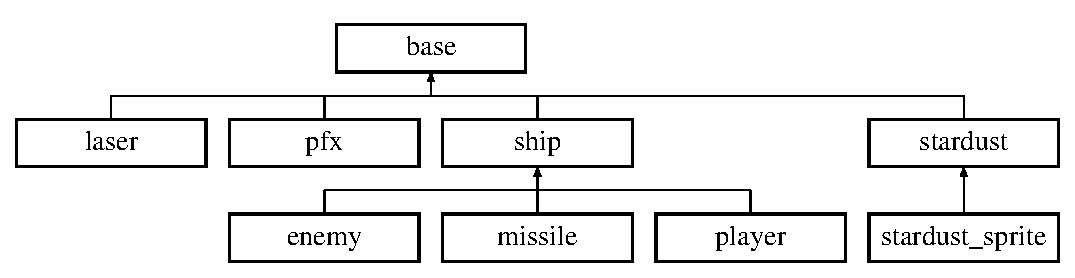
\includegraphics[height=3.000000cm]{classbase}
\end{center}
\end{figure}
\subsection*{Public Member Functions}
\begin{DoxyCompactItemize}
\item 
\hypertarget{classbase_a90093f488dc92a1eede40eb47b622ef7}{void \hyperlink{classbase_a90093f488dc92a1eede40eb47b622ef7}{set\-Pos} (const \hyperlink{structvec3}{vec3} \-\_\-val)}\label{classbase_a90093f488dc92a1eede40eb47b622ef7}

\begin{DoxyCompactList}\small\item\em Getters and setters for position. \end{DoxyCompactList}\item 
\hypertarget{classbase_aeaa2eadbc7b45eceadb5a4c2af2e8933}{void {\bfseries add\-Pos} (const \hyperlink{structvec3}{vec3} \-\_\-vec)}\label{classbase_aeaa2eadbc7b45eceadb5a4c2af2e8933}

\item 
\hypertarget{classbase_ac76c779722a45ea5d1b2acacffc89d3a}{\hyperlink{structvec3}{vec3} {\bfseries get\-Pos} () const }\label{classbase_ac76c779722a45ea5d1b2acacffc89d3a}

\item 
\hypertarget{classbase_a3813c5f44f3353e0e5561e034b0d77c4}{\hyperlink{structvec3}{vec3} \hyperlink{classbase_a3813c5f44f3353e0e5561e034b0d77c4}{get\-P\-Pos} () const }\label{classbase_a3813c5f44f3353e0e5561e034b0d77c4}

\begin{DoxyCompactList}\small\item\em Getters and setters for m\-\_\-prev\-Pos. \end{DoxyCompactList}\item 
\hypertarget{classbase_ac445f374b2d57f6c5bb034cda3a340e2}{void {\bfseries set\-P\-Pos} (const \hyperlink{structvec3}{vec3} \-\_\-p)}\label{classbase_ac445f374b2d57f6c5bb034cda3a340e2}

\item 
\hypertarget{classbase_a55f39acb84460ec5cc72793d96515593}{void \hyperlink{classbase_a55f39acb84460ec5cc72793d96515593}{set\-Vel} (const \hyperlink{structvec3}{vec3} \-\_\-v)}\label{classbase_a55f39acb84460ec5cc72793d96515593}

\begin{DoxyCompactList}\small\item\em Setters for velocity. \end{DoxyCompactList}\item 
\hypertarget{classbase_abb66dade6add41fd6a85cb1052486127}{void {\bfseries set\-W\-Vel} (const \hyperlink{structvec3}{vec3} \-\_\-wv)}\label{classbase_abb66dade6add41fd6a85cb1052486127}

\item 
\hypertarget{classbase_aa55d4885e976c58b056b5bdb57ec81c6}{void {\bfseries add\-Vel} (const \hyperlink{structvec3}{vec3} \-\_\-v)}\label{classbase_aa55d4885e976c58b056b5bdb57ec81c6}

\item 
\hypertarget{classbase_a650afb671306510b180db4dc30c9f292}{\hyperlink{structvec3}{vec3} \hyperlink{classbase_a650afb671306510b180db4dc30c9f292}{get\-Vel} () const }\label{classbase_a650afb671306510b180db4dc30c9f292}

\begin{DoxyCompactList}\small\item\em Getters for velocity. \end{DoxyCompactList}\item 
\hypertarget{classbase_a54695a44b9266342f510130ffc440ca2}{\hyperlink{structvec3}{vec3} {\bfseries get\-W\-Vel} () const }\label{classbase_a54695a44b9266342f510130ffc440ca2}

\item 
void \hyperlink{classbase_abdbbabe4760b3b4b163218f1e0191158}{update\-Pos} (float \-\_\-dt)
\begin{DoxyCompactList}\small\item\em Updates the position of the object based on velocity, wvel, and time differece. \end{DoxyCompactList}\item 
\hyperlink{structvec3}{vec3} \hyperlink{classbase_ace83be5af90e232274c63a2e56fd3b15}{get\-Interpolated\-Position} (const float \-\_\-dt)
\begin{DoxyCompactList}\small\item\em Returns a \hyperlink{structvec2}{vec2} interpolated between current and previous position. \end{DoxyCompactList}\end{DoxyCompactItemize}


\subsection{Detailed Description}
Contains position and velocity, and the functionality to update based on time difference. 

\subsection{Member Function Documentation}
\hypertarget{classbase_ace83be5af90e232274c63a2e56fd3b15}{\index{base@{base}!get\-Interpolated\-Position@{get\-Interpolated\-Position}}
\index{get\-Interpolated\-Position@{get\-Interpolated\-Position}!base@{base}}
\subsubsection[{get\-Interpolated\-Position}]{\setlength{\rightskip}{0pt plus 5cm}{\bf vec3} base\-::get\-Interpolated\-Position (
\begin{DoxyParamCaption}
\item[{const float}]{\-\_\-dt}
\end{DoxyParamCaption}
)}}\label{classbase_ace83be5af90e232274c63a2e56fd3b15}


Returns a \hyperlink{structvec2}{vec2} interpolated between current and previous position. 


\begin{DoxyParams}{Parameters}
{\em \-\_\-dt} & interpolant \\
\hline
\end{DoxyParams}
\hypertarget{classbase_abdbbabe4760b3b4b163218f1e0191158}{\index{base@{base}!update\-Pos@{update\-Pos}}
\index{update\-Pos@{update\-Pos}!base@{base}}
\subsubsection[{update\-Pos}]{\setlength{\rightskip}{0pt plus 5cm}void base\-::update\-Pos (
\begin{DoxyParamCaption}
\item[{float}]{\-\_\-dt}
\end{DoxyParamCaption}
)}}\label{classbase_abdbbabe4760b3b4b163218f1e0191158}


Updates the position of the object based on velocity, wvel, and time differece. 


\begin{DoxyParams}{Parameters}
{\em \-\_\-dt} & the time difference since the last update. \\
\hline
\end{DoxyParams}


The documentation for this class was generated from the following files\-:\begin{DoxyCompactItemize}
\item 
include/\hyperlink{base_8hpp}{base.\-hpp}\item 
src/base.\-cpp\end{DoxyCompactItemize}

\hypertarget{classui_1_1button}{\section{ui\-:\-:button Class Reference}
\label{classui_1_1button}\index{ui\-::button@{ui\-::button}}
}
\subsection*{Public Member Functions}
\begin{DoxyCompactItemize}
\item 
\hyperlink{classui_1_1button_aa6e3eea4dcc22983d7ae1b0b0121850f}{button} (const std\-::string \-\_\-label, const std\-::array$<$ int, 8 $>$ \-\_\-pcol, const std\-::array$<$ int, 8 $>$ \-\_\-tcol, const \hyperlink{structvec2}{vec2} \-\_\-pos, const \hyperlink{structvec2}{vec2} \-\_\-dim)
\begin{DoxyCompactList}\small\item\em ctor for the button class. \end{DoxyCompactList}\item 
\hyperlink{classui_1_1button_aaa5b4acc8a3088a7dbc18612c4b7f165}{button} (const std\-::string \-\_\-label, const std\-::array$<$ int, 8 $>$ \-\_\-pcol, const std\-::array$<$ int, 8 $>$ \-\_\-tcol, const \hyperlink{structvec2}{vec2} \-\_\-pos, const \hyperlink{structvec2}{vec2} \-\_\-dim, const float \-\_\-smul)
\begin{DoxyCompactList}\small\item\em ctor for the button class. \end{DoxyCompactList}\item 
\hyperlink{classui_1_1button_a3a8746c1243b69585e68c546ad5c769a}{button} (const std\-::string \-\_\-label, std\-::array$<$ int, 8 $>$ \-\_\-pcol, std\-::array$<$ int, 8 $>$ \-\_\-tcol, \hyperlink{structvec2}{vec2} \-\_\-pos, \hyperlink{structvec2}{vec2} \-\_\-dim, int \-\_\-pcost)
\begin{DoxyCompactList}\small\item\em ctor for the button class. \end{DoxyCompactList}\item 
\hypertarget{classui_1_1button_a45aefd446962e88d8f4c0826ae5709ec}{void \hyperlink{classui_1_1button_a45aefd446962e88d8f4c0826ae5709ec}{select} ()}\label{classui_1_1button_a45aefd446962e88d8f4c0826ae5709ec}

\begin{DoxyCompactList}\small\item\em Selects the button. \end{DoxyCompactList}\item 
void \hyperlink{classui_1_1button_a8068afa66f15f7fa29ab5dadbff88909}{update\-Text} (const std\-::string \-\_\-str)
\begin{DoxyCompactList}\small\item\em Setter for m\-\_\-label. \end{DoxyCompactList}\item 
\hypertarget{classui_1_1button_a85fb38ca3fbf644d64829145f2d6f588}{void \hyperlink{classui_1_1button_a85fb38ca3fbf644d64829145f2d6f588}{set} (bool s)}\label{classui_1_1button_a85fb38ca3fbf644d64829145f2d6f588}

\begin{DoxyCompactList}\small\item\em Getter and setter for m\-\_\-selected. \end{DoxyCompactList}\item 
\hypertarget{classui_1_1button_a28126c764f0c4f4bd7959710d1b17f96}{bool {\bfseries on} ()}\label{classui_1_1button_a28126c764f0c4f4bd7959710d1b17f96}

\item 
void \hyperlink{classui_1_1button_a2800d76e1353204c765457712b660738}{update} (int \-\_\-s)
\begin{DoxyCompactList}\small\item\em Updates the button. \end{DoxyCompactList}\item 
\hypertarget{classui_1_1button_a700f316bbee15cad1ae63b81b5c5073f}{int \hyperlink{classui_1_1button_a700f316bbee15cad1ae63b81b5c5073f}{get\-Cost} ()}\label{classui_1_1button_a700f316bbee15cad1ae63b81b5c5073f}

\begin{DoxyCompactList}\small\item\em Getter and setter for cost. \end{DoxyCompactList}\item 
\hypertarget{classui_1_1button_ac980f616aa93bc533d95a0e195b5987e}{void {\bfseries set\-Cost} (int pcost)}\label{classui_1_1button_ac980f616aa93bc533d95a0e195b5987e}

\item 
\hypertarget{classui_1_1button_ad0a516f7c5fc2870a2dc7d9d46c011dd}{void \hyperlink{classui_1_1button_ad0a516f7c5fc2870a2dc7d9d46c011dd}{set\-Dark} (bool b)}\label{classui_1_1button_ad0a516f7c5fc2870a2dc7d9d46c011dd}

\begin{DoxyCompactList}\small\item\em Getter and setter for clickability. \end{DoxyCompactList}\item 
\hypertarget{classui_1_1button_a3350df4e21ddd0a80b03a3931fbe3cfa}{bool {\bfseries is\-Dark} ()}\label{classui_1_1button_a3350df4e21ddd0a80b03a3931fbe3cfa}

\item 
\hypertarget{classui_1_1button_a9f4a8a3e03d0eefe4359fa1d42df19b0}{\hyperlink{structvec2}{vec2} \hyperlink{classui_1_1button_a9f4a8a3e03d0eefe4359fa1d42df19b0}{get\-Pos} ()}\label{classui_1_1button_a9f4a8a3e03d0eefe4359fa1d42df19b0}

\begin{DoxyCompactList}\small\item\em Getter for position. \end{DoxyCompactList}\item 
\hypertarget{classui_1_1button_ae2d328b1a97d25cf1379c7b2fd01d2f1}{\hyperlink{structvec2}{vec2} \hyperlink{classui_1_1button_ae2d328b1a97d25cf1379c7b2fd01d2f1}{get\-Dim} ()}\label{classui_1_1button_ae2d328b1a97d25cf1379c7b2fd01d2f1}

\begin{DoxyCompactList}\small\item\em Getter for dimensions. \end{DoxyCompactList}\item 
\hypertarget{classui_1_1button_ab8b1a929809c025152fd3151cb6725a3}{std\-::array$<$ float, 4 $>$ \hyperlink{classui_1_1button_ab8b1a929809c025152fd3151cb6725a3}{get\-Draw\-Col} ()}\label{classui_1_1button_ab8b1a929809c025152fd3151cb6725a3}

\begin{DoxyCompactList}\small\item\em Getter for draw colour. \end{DoxyCompactList}\item 
\hypertarget{classui_1_1button_a703993eaab990656c3eaafb7d1aab8ce}{std\-::array$<$ int, 8 $>$ \hyperlink{classui_1_1button_a703993eaab990656c3eaafb7d1aab8ce}{get\-Col} ()}\label{classui_1_1button_a703993eaab990656c3eaafb7d1aab8ce}

\begin{DoxyCompactList}\small\item\em Getter for background colour. \end{DoxyCompactList}\item 
\hypertarget{classui_1_1button_a77e6e79bf186ea33bc0f7d1b7b88ba71}{std\-::array$<$ int, 8 $>$ \hyperlink{classui_1_1button_a77e6e79bf186ea33bc0f7d1b7b88ba71}{get\-T\-Col} ()}\label{classui_1_1button_a77e6e79bf186ea33bc0f7d1b7b88ba71}

\begin{DoxyCompactList}\small\item\em Getter for text colour. \end{DoxyCompactList}\item 
\hypertarget{classui_1_1button_aafa157c40fcc2c7eda8162d9ca2c672d}{std\-::string \hyperlink{classui_1_1button_aafa157c40fcc2c7eda8162d9ca2c672d}{get\-Label} ()}\label{classui_1_1button_aafa157c40fcc2c7eda8162d9ca2c672d}

\begin{DoxyCompactList}\small\item\em Getter for label. \end{DoxyCompactList}\item 
\hypertarget{classui_1_1button_a80d9d9b553f9c2399267da4bdb484bfa}{void \hyperlink{classui_1_1button_a80d9d9b553f9c2399267da4bdb484bfa}{reset} ()}\label{classui_1_1button_a80d9d9b553f9c2399267da4bdb484bfa}

\begin{DoxyCompactList}\small\item\em Resets the button to its initial state. \end{DoxyCompactList}\item 
\hypertarget{classui_1_1button_ac0bca6348e2cad990d510fb4246fa36f}{float \hyperlink{classui_1_1button_ac0bca6348e2cad990d510fb4246fa36f}{get\-Text\-Size\-Mul} ()}\label{classui_1_1button_ac0bca6348e2cad990d510fb4246fa36f}

\begin{DoxyCompactList}\small\item\em Getter for text size multiplier. \end{DoxyCompactList}\end{DoxyCompactItemize}


\subsection{Constructor \& Destructor Documentation}
\hypertarget{classui_1_1button_aa6e3eea4dcc22983d7ae1b0b0121850f}{\index{ui\-::button@{ui\-::button}!button@{button}}
\index{button@{button}!ui::button@{ui\-::button}}
\subsubsection[{button}]{\setlength{\rightskip}{0pt plus 5cm}button\-::button (
\begin{DoxyParamCaption}
\item[{const std\-::string}]{\-\_\-label, }
\item[{const std\-::array$<$ int, 8 $>$}]{\-\_\-pcol, }
\item[{const std\-::array$<$ int, 8 $>$}]{\-\_\-tcol, }
\item[{const {\bf vec2}}]{\-\_\-pos, }
\item[{const {\bf vec2}}]{\-\_\-dim}
\end{DoxyParamCaption}
)}}\label{classui_1_1button_aa6e3eea4dcc22983d7ae1b0b0121850f}


ctor for the button class. 


\begin{DoxyParams}{Parameters}
{\em \-\_\-label} & button text. \\
\hline
{\em \-\_\-pcol} & background colour. \\
\hline
{\em \-\_\-tcol} & text colour. \\
\hline
{\em \-\_\-pos} & position. \\
\hline
{\em \-\_\-dim} & dimensions. \\
\hline
\end{DoxyParams}
\hypertarget{classui_1_1button_aaa5b4acc8a3088a7dbc18612c4b7f165}{\index{ui\-::button@{ui\-::button}!button@{button}}
\index{button@{button}!ui::button@{ui\-::button}}
\subsubsection[{button}]{\setlength{\rightskip}{0pt plus 5cm}button\-::button (
\begin{DoxyParamCaption}
\item[{const std\-::string}]{\-\_\-label, }
\item[{const std\-::array$<$ int, 8 $>$}]{\-\_\-pcol, }
\item[{const std\-::array$<$ int, 8 $>$}]{\-\_\-tcol, }
\item[{const {\bf vec2}}]{\-\_\-pos, }
\item[{const {\bf vec2}}]{\-\_\-dim, }
\item[{const float}]{\-\_\-smul}
\end{DoxyParamCaption}
)}}\label{classui_1_1button_aaa5b4acc8a3088a7dbc18612c4b7f165}


ctor for the button class. 


\begin{DoxyParams}{Parameters}
{\em \-\_\-label} & button text. \\
\hline
{\em \-\_\-pcol} & background colour. \\
\hline
{\em \-\_\-tcol} & text colour. \\
\hline
{\em \-\_\-pos} & position. \\
\hline
{\em \-\_\-dim} & dimensions. \\
\hline
{\em \-\_\-smul} & size mult for the button text. \\
\hline
\end{DoxyParams}
\hypertarget{classui_1_1button_a3a8746c1243b69585e68c546ad5c769a}{\index{ui\-::button@{ui\-::button}!button@{button}}
\index{button@{button}!ui::button@{ui\-::button}}
\subsubsection[{button}]{\setlength{\rightskip}{0pt plus 5cm}button\-::button (
\begin{DoxyParamCaption}
\item[{const std\-::string}]{\-\_\-label, }
\item[{std\-::array$<$ int, 8 $>$}]{\-\_\-pcol, }
\item[{std\-::array$<$ int, 8 $>$}]{\-\_\-tcol, }
\item[{{\bf vec2}}]{\-\_\-pos, }
\item[{{\bf vec2}}]{\-\_\-dim, }
\item[{int}]{\-\_\-pcost}
\end{DoxyParamCaption}
)}}\label{classui_1_1button_a3a8746c1243b69585e68c546ad5c769a}


ctor for the button class. 


\begin{DoxyParams}{Parameters}
{\em \-\_\-label} & button text, \\
\hline
{\em \-\_\-pcol} & background colour. \\
\hline
{\em \-\_\-tcol} & text colour. \\
\hline
{\em \-\_\-pos} & position. \\
\hline
{\em \-\_\-dim} & dimensions. \\
\hline
{\em \-\_\-pcost} & button cost. \\
\hline
\end{DoxyParams}


\subsection{Member Function Documentation}
\hypertarget{classui_1_1button_a2800d76e1353204c765457712b660738}{\index{ui\-::button@{ui\-::button}!update@{update}}
\index{update@{update}!ui::button@{ui\-::button}}
\subsubsection[{update}]{\setlength{\rightskip}{0pt plus 5cm}void button\-::update (
\begin{DoxyParamCaption}
\item[{int}]{\-\_\-s}
\end{DoxyParamCaption}
)}}\label{classui_1_1button_a2800d76e1353204c765457712b660738}


Updates the button. 


\begin{DoxyParams}{Parameters}
{\em \-\_\-s} & current score. \\
\hline
\end{DoxyParams}
\hypertarget{classui_1_1button_a8068afa66f15f7fa29ab5dadbff88909}{\index{ui\-::button@{ui\-::button}!update\-Text@{update\-Text}}
\index{update\-Text@{update\-Text}!ui::button@{ui\-::button}}
\subsubsection[{update\-Text}]{\setlength{\rightskip}{0pt plus 5cm}void button\-::update\-Text (
\begin{DoxyParamCaption}
\item[{const std\-::string}]{\-\_\-str}
\end{DoxyParamCaption}
)}}\label{classui_1_1button_a8068afa66f15f7fa29ab5dadbff88909}


Setter for m\-\_\-label. 

update\-Text 
\begin{DoxyParams}{Parameters}
{\em \-\_\-str} & \\
\hline
\end{DoxyParams}


The documentation for this class was generated from the following files\-:\begin{DoxyCompactItemize}
\item 
include/ui/\hyperlink{button_8hpp}{button.\-hpp}\item 
src/ui/button.\-cpp\end{DoxyCompactItemize}

\hypertarget{classbutton}{\section{button Class Reference}
\label{classbutton}\index{button@{button}}
}


Contains attributes such as colour, label and position.  




{\ttfamily \#include $<$button.\-hpp$>$}



\subsection{Detailed Description}
Contains attributes such as colour, label and position. 

The documentation for this class was generated from the following file\-:\begin{DoxyCompactItemize}
\item 
include/ui/\hyperlink{button_8hpp}{button.\-hpp}\end{DoxyCompactItemize}

\hypertarget{structcol__partition}{\section{col\-\_\-partition Class Reference}
\label{structcol__partition}\index{col\-\_\-partition@{col\-\_\-partition}}
}


\hyperlink{struct_a}{A} simple struct, designed to hold a group of entities in close proximity to one another, who can interact in some way.  




{\ttfamily \#include $<$universe.\-hpp$>$}

\subsection*{Public Attributes}
\begin{DoxyCompactItemize}
\item 
\hypertarget{structcol__partition_ab69905db296ca37408dbe6f1ab011a26}{std\-::vector$<$ std\-::vector\\*
$<$ \hyperlink{classenemy}{enemy} $\ast$ $>$ $>$ \hyperlink{structcol__partition_ab69905db296ca37408dbe6f1ab011a26}{ships}}\label{structcol__partition_ab69905db296ca37408dbe6f1ab011a26}

\begin{DoxyCompactList}\small\item\em Vector of ship references. \end{DoxyCompactList}\item 
\hypertarget{structcol__partition_a0afda4d9265e546a9d7a99688ed86106}{std\-::vector$<$ std\-::vector\\*
$<$ \hyperlink{classlaser}{laser} $\ast$ $>$ $>$ \hyperlink{structcol__partition_a0afda4d9265e546a9d7a99688ed86106}{lasers}}\label{structcol__partition_a0afda4d9265e546a9d7a99688ed86106}

\begin{DoxyCompactList}\small\item\em Vector of laser references. \end{DoxyCompactList}\item 
\hypertarget{structcol__partition_a254fbb79574d28efe247fb4fcd57b049}{std\-::vector$<$ std\-::vector\\*
$<$ \hyperlink{classmissile}{missile} $\ast$ $>$ $>$ \hyperlink{structcol__partition_a254fbb79574d28efe247fb4fcd57b049}{rockets}}\label{structcol__partition_a254fbb79574d28efe247fb4fcd57b049}

\begin{DoxyCompactList}\small\item\em Vector of missile references. \end{DoxyCompactList}\item 
\hypertarget{structcol__partition_a0cc367dfcae1067c859e3445454ca071}{std\-::vector$<$ std\-::vector$<$ \hyperlink{classship}{ship} $\ast$ $>$ $>$ \hyperlink{structcol__partition_a0cc367dfcae1067c859e3445454ca071}{rocks}}\label{structcol__partition_a0cc367dfcae1067c859e3445454ca071}

\begin{DoxyCompactList}\small\item\em Vector of asteroid references. \end{DoxyCompactList}\end{DoxyCompactItemize}


\subsection{Detailed Description}
\hyperlink{struct_a}{A} simple struct, designed to hold a group of entities in close proximity to one another, who can interact in some way. 

The documentation for this class was generated from the following file\-:\begin{DoxyCompactItemize}
\item 
include/\hyperlink{universe_8hpp}{universe.\-hpp}\end{DoxyCompactItemize}

\hypertarget{struct_container}{\section{Container Struct Reference}
\label{struct_container}\index{Container@{Container}}
}


euler angle with pitch yaw and roll. Not finished.  




\subsection{Detailed Description}
euler angle with pitch yaw and roll. Not finished. 

The documentation for this struct was generated from the following file\-:\begin{DoxyCompactItemize}
\item 
include/vectors.\-hpp\end{DoxyCompactItemize}

\hypertarget{classenemy}{\section{enemy Class Reference}
\label{classenemy}\index{enemy@{enemy}}
}


Builds upon the ship class, adding variables like team, goal, targets etc.  




{\ttfamily \#include $<$enemy.\-hpp$>$}

Inheritance diagram for enemy\-:\begin{figure}[H]
\begin{center}
\leavevmode
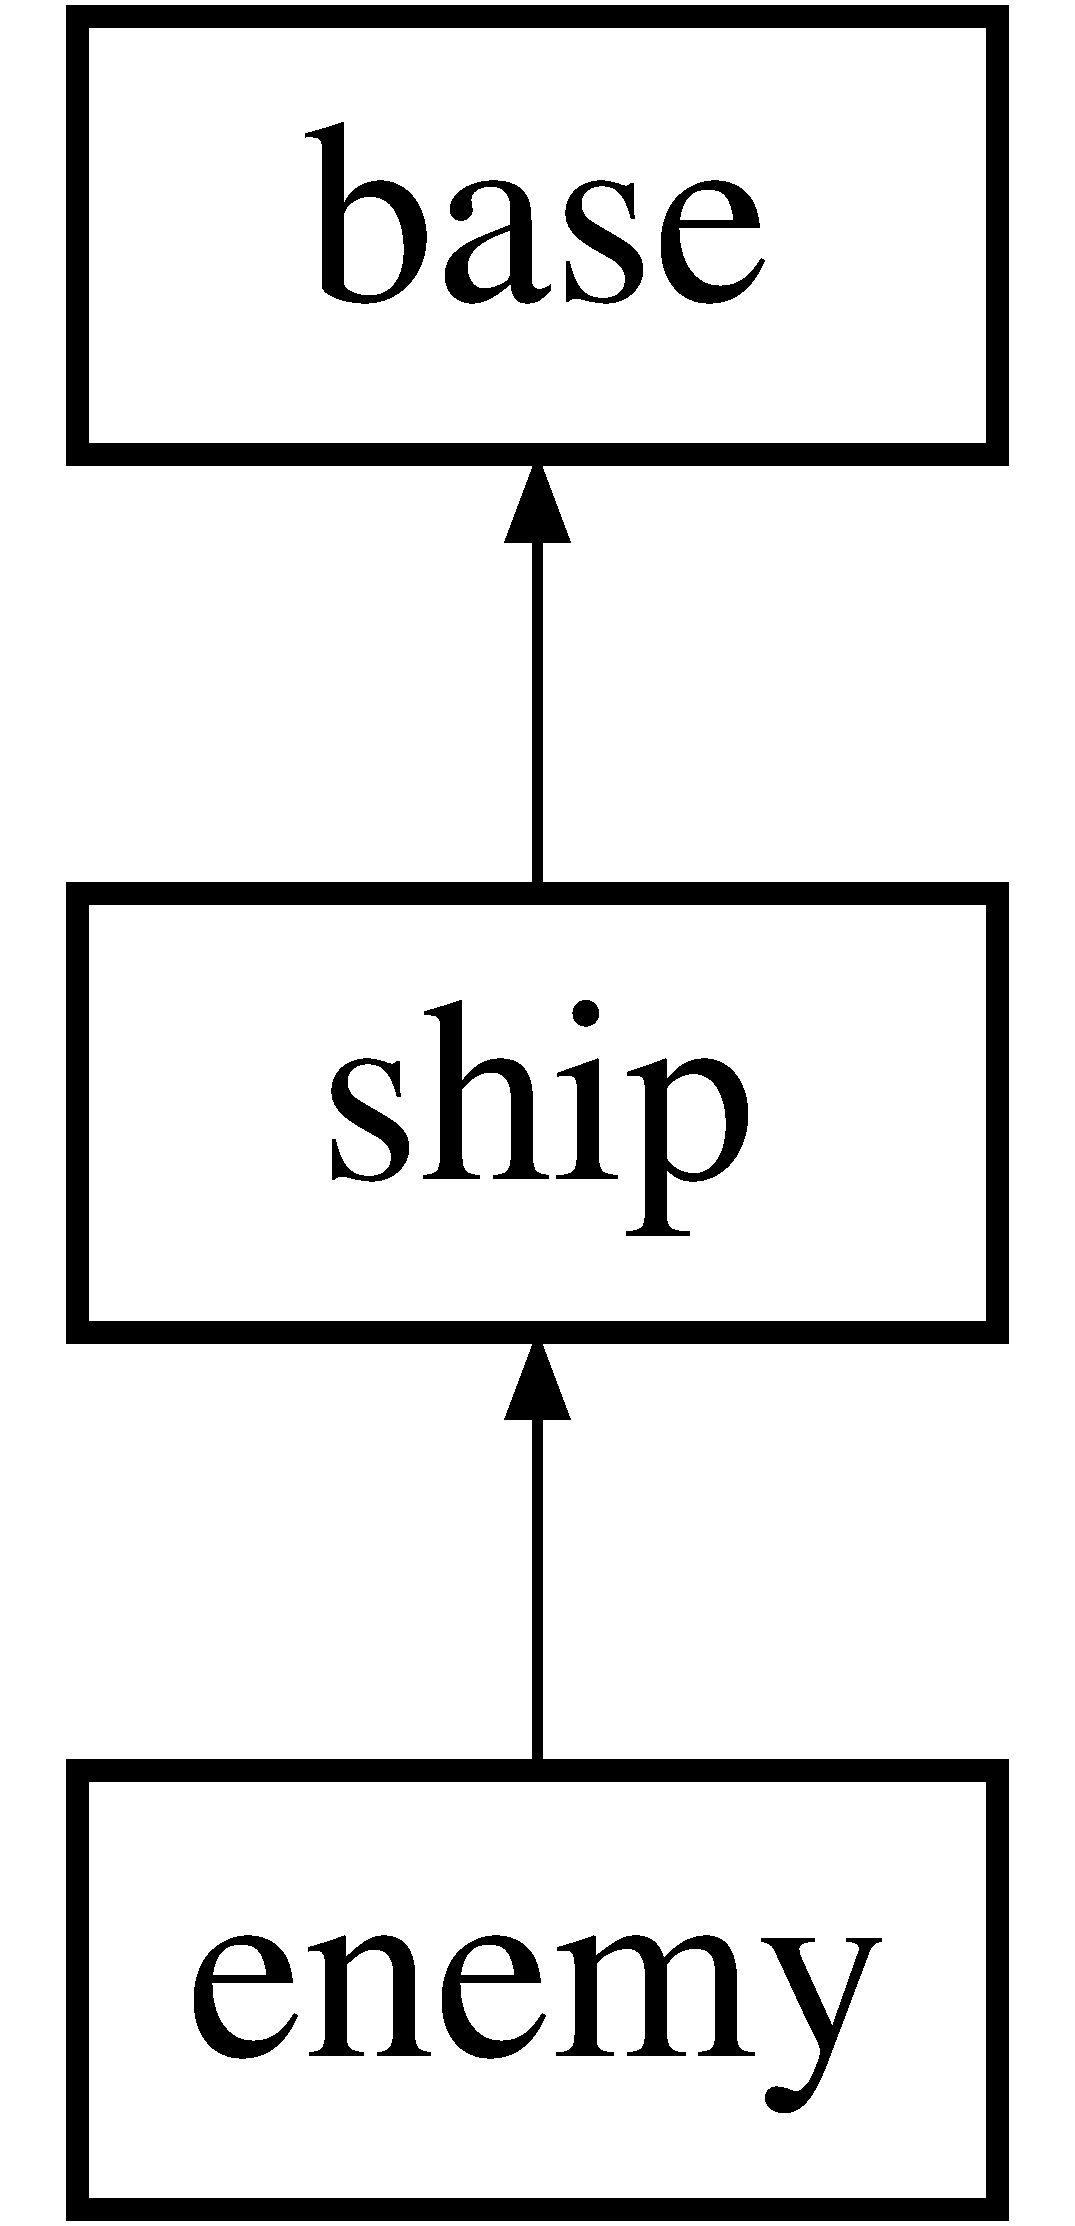
\includegraphics[height=3.000000cm]{classenemy}
\end{center}
\end{figure}
\subsection*{Public Member Functions}
\begin{DoxyCompactItemize}
\item 
\hyperlink{classenemy_acca194a2f379300a8ee019ab3bb36298}{enemy} (const \hyperlink{structvec3}{vec3} \-\_\-p, const \hyperlink{structvec3}{vec3} \-\_\-v, const \hyperlink{ship_8hpp_af74a63841701826d661cb9809aaf7092}{ship\-\_\-spec} \-\_\-type, const \hyperlink{enemy_8hpp_abac1fdbabb5a6be5f0d6ae40be5c5a58}{ai\-Team} \-\_\-team)
\begin{DoxyCompactList}\small\item\em ctor for the enemy class \end{DoxyCompactList}\item 
\hypertarget{classenemy_a98c55268826433d0b9ad4b1f1e7075fa}{void \hyperlink{classenemy_a98c55268826433d0b9ad4b1f1e7075fa}{set\-Goal} (\hyperlink{enemy_8hpp_a6e73eb3e8e86f5922e45adeb450ceb1e}{ai\-Goal} \-\_\-g)}\label{classenemy_a98c55268826433d0b9ad4b1f1e7075fa}

\begin{DoxyCompactList}\small\item\em Getter and setter for curent goal. \end{DoxyCompactList}\item 
\hypertarget{classenemy_a0cda47391d310982f33059297f6aa947}{\hyperlink{enemy_8hpp_a6e73eb3e8e86f5922e45adeb450ceb1e}{ai\-Goal} {\bfseries get\-Goal} ()}\label{classenemy_a0cda47391d310982f33059297f6aa947}

\item 
void \hyperlink{classenemy_a98c0bb6881129829530c2dddb46e7c3b}{behvr\-Update} (float \-\_\-dt)
\begin{DoxyCompactList}\small\item\em Updates the behaviour of the agent, based on any target it has, and its relative position. \end{DoxyCompactList}\item 
\hypertarget{classenemy_a335001d4aa50011d3031f637cc8bc19f}{void \hyperlink{classenemy_a335001d4aa50011d3031f637cc8bc19f}{steering} ()}\label{classenemy_a335001d4aa50011d3031f637cc8bc19f}

\begin{DoxyCompactList}\small\item\em Applies forces to the agent, attempting to steer it towards the target. \end{DoxyCompactList}\item 
\hypertarget{classenemy_a3d219aef97dd32ff974b67301875b553}{\hyperlink{enemy_8hpp_abac1fdbabb5a6be5f0d6ae40be5c5a58}{ai\-Team} \hyperlink{classenemy_a3d219aef97dd32ff974b67301875b553}{get\-Team} () const }\label{classenemy_a3d219aef97dd32ff974b67301875b553}

\begin{DoxyCompactList}\small\item\em Getter and setter for the team. \end{DoxyCompactList}\item 
\hypertarget{classenemy_a38fea22ce884d392db8a48e91cdbfc44}{void {\bfseries set\-Team} (const \hyperlink{enemy_8hpp_abac1fdbabb5a6be5f0d6ae40be5c5a58}{ai\-Team} \-\_\-t)}\label{classenemy_a38fea22ce884d392db8a48e91cdbfc44}

\item 
\hypertarget{classenemy_a8e33a832e8a4d8fb36b5515d9a135100}{\hyperlink{classship}{ship} $\ast$ \hyperlink{classenemy_a8e33a832e8a4d8fb36b5515d9a135100}{get\-Target} () const }\label{classenemy_a8e33a832e8a4d8fb36b5515d9a135100}

\begin{DoxyCompactList}\small\item\em Getter and setter for the target. \end{DoxyCompactList}\item 
\hypertarget{classenemy_a4e1afdb5ec33f9a822274f4a91c08fb4}{void {\bfseries set\-Target} (\hyperlink{classship}{ship} $\ast$\-\_\-t)}\label{classenemy_a4e1afdb5ec33f9a822274f4a91c08fb4}

\item 
\hypertarget{classenemy_aa5c138596d70d5a05198706dc9bda3f2}{float \hyperlink{classenemy_aa5c138596d70d5a05198706dc9bda3f2}{get\-Confidence} ()}\label{classenemy_aa5c138596d70d5a05198706dc9bda3f2}

\begin{DoxyCompactList}\small\item\em Getters and setters for confidence. \end{DoxyCompactList}\item 
\hypertarget{classenemy_a9286b2d085a9a4ce18ad4e8c8fa8c9b1}{void {\bfseries set\-Confidence} (float c)}\label{classenemy_a9286b2d085a9a4ce18ad4e8c8fa8c9b1}

\item 
\hypertarget{classenemy_af1ae4819d9fc4618a43a63aca51846df}{void {\bfseries decr\-Confidence} (float d)}\label{classenemy_af1ae4819d9fc4618a43a63aca51846df}

\item 
\hypertarget{classenemy_ab0816a768444fd9882eeff8a6c029c11}{int \hyperlink{classenemy_ab0816a768444fd9882eeff8a6c029c11}{get\-Squad\-I\-D} () const }\label{classenemy_ab0816a768444fd9882eeff8a6c029c11}

\begin{DoxyCompactList}\small\item\em Getter and setter for squad id. \end{DoxyCompactList}\item 
\hypertarget{classenemy_a5671bad5043e8c2501f25953e3926a33}{void {\bfseries set\-Squad\-I\-D} (int \-\_\-id)}\label{classenemy_a5671bad5043e8c2501f25953e3926a33}

\item 
\hypertarget{classenemy_ab8d678715024ec30ee700ffa58c4dae9}{void \hyperlink{classenemy_ab8d678715024ec30ee700ffa58c4dae9}{set\-T\-Pos} (\hyperlink{structvec3}{vec3} \-\_\-t\-Pos)}\label{classenemy_ab8d678715024ec30ee700ffa58c4dae9}

\begin{DoxyCompactList}\small\item\em Getter and setter for the target position. \end{DoxyCompactList}\item 
\hypertarget{classenemy_ad9c48b05b1055edbbd583188a0782466}{void {\bfseries set\-T\-Vel} (\hyperlink{structvec3}{vec3} \-\_\-t\-Vel)}\label{classenemy_ad9c48b05b1055edbbd583188a0782466}

\end{DoxyCompactItemize}


\subsection{Detailed Description}
Builds upon the ship class, adding variables like team, goal, targets etc. 

\subsection{Constructor \& Destructor Documentation}
\hypertarget{classenemy_acca194a2f379300a8ee019ab3bb36298}{\index{enemy@{enemy}!enemy@{enemy}}
\index{enemy@{enemy}!enemy@{enemy}}
\subsubsection[{enemy}]{\setlength{\rightskip}{0pt plus 5cm}enemy\-::enemy (
\begin{DoxyParamCaption}
\item[{const {\bf vec3}}]{\-\_\-p, }
\item[{const {\bf vec3}}]{\-\_\-v, }
\item[{const {\bf ship\-\_\-spec}}]{\-\_\-type, }
\item[{const {\bf ai\-Team}}]{\-\_\-team}
\end{DoxyParamCaption}
)}}\label{classenemy_acca194a2f379300a8ee019ab3bb36298}


ctor for the enemy class 


\begin{DoxyParams}{Parameters}
{\em \-\_\-p} & position \\
\hline
{\em \-\_\-v} & velocity \\
\hline
{\em \-\_\-type} & the ship type (defined in the ship header) \\
\hline
{\em \-\_\-team} & the ai team of this agent \\
\hline
\end{DoxyParams}


\subsection{Member Function Documentation}
\hypertarget{classenemy_a98c0bb6881129829530c2dddb46e7c3b}{\index{enemy@{enemy}!behvr\-Update@{behvr\-Update}}
\index{behvr\-Update@{behvr\-Update}!enemy@{enemy}}
\subsubsection[{behvr\-Update}]{\setlength{\rightskip}{0pt plus 5cm}void enemy\-::behvr\-Update (
\begin{DoxyParamCaption}
\item[{float}]{\-\_\-dt}
\end{DoxyParamCaption}
)}}\label{classenemy_a98c0bb6881129829530c2dddb46e7c3b}


Updates the behaviour of the agent, based on any target it has, and its relative position. 


\begin{DoxyParams}{Parameters}
{\em \-\_\-dt} & time difference since last update \\
\hline
\end{DoxyParams}


The documentation for this class was generated from the following files\-:\begin{DoxyCompactItemize}
\item 
include/\hyperlink{enemy_8hpp}{enemy.\-hpp}\item 
src/enemy.\-cpp\end{DoxyCompactItemize}

\hypertarget{structfaction}{\section{faction Struct Reference}
\label{structfaction}\index{faction@{faction}}
}


Barebones implementation of factions, currently only contains colour.  




{\ttfamily \#include $<$faction.\-hpp$>$}

\subsection*{Public Attributes}
\begin{DoxyCompactItemize}
\item 
\hypertarget{structfaction_a05566e5c37033a6a895cd64ff5ce5479}{std\-::array$<$ int, 4 $>$ \hyperlink{structfaction_a05566e5c37033a6a895cd64ff5ce5479}{m\-\_\-colour}}\label{structfaction_a05566e5c37033a6a895cd64ff5ce5479}

\begin{DoxyCompactList}\small\item\em Faction colour. \end{DoxyCompactList}\end{DoxyCompactItemize}


\subsection{Detailed Description}
Barebones implementation of factions, currently only contains colour. 

The documentation for this struct was generated from the following file\-:\begin{DoxyCompactItemize}
\item 
include/\hyperlink{faction_8hpp}{faction.\-hpp}\end{DoxyCompactItemize}

\hypertarget{classlaser}{\section{laser Class Reference}
\label{classlaser}\index{laser@{laser}}
}


Inherits from base, represents a laser and contains data such as faction, damage, colour etc.  




{\ttfamily \#include $<$laser.\-hpp$>$}

Inheritance diagram for laser\-:\begin{figure}[H]
\begin{center}
\leavevmode
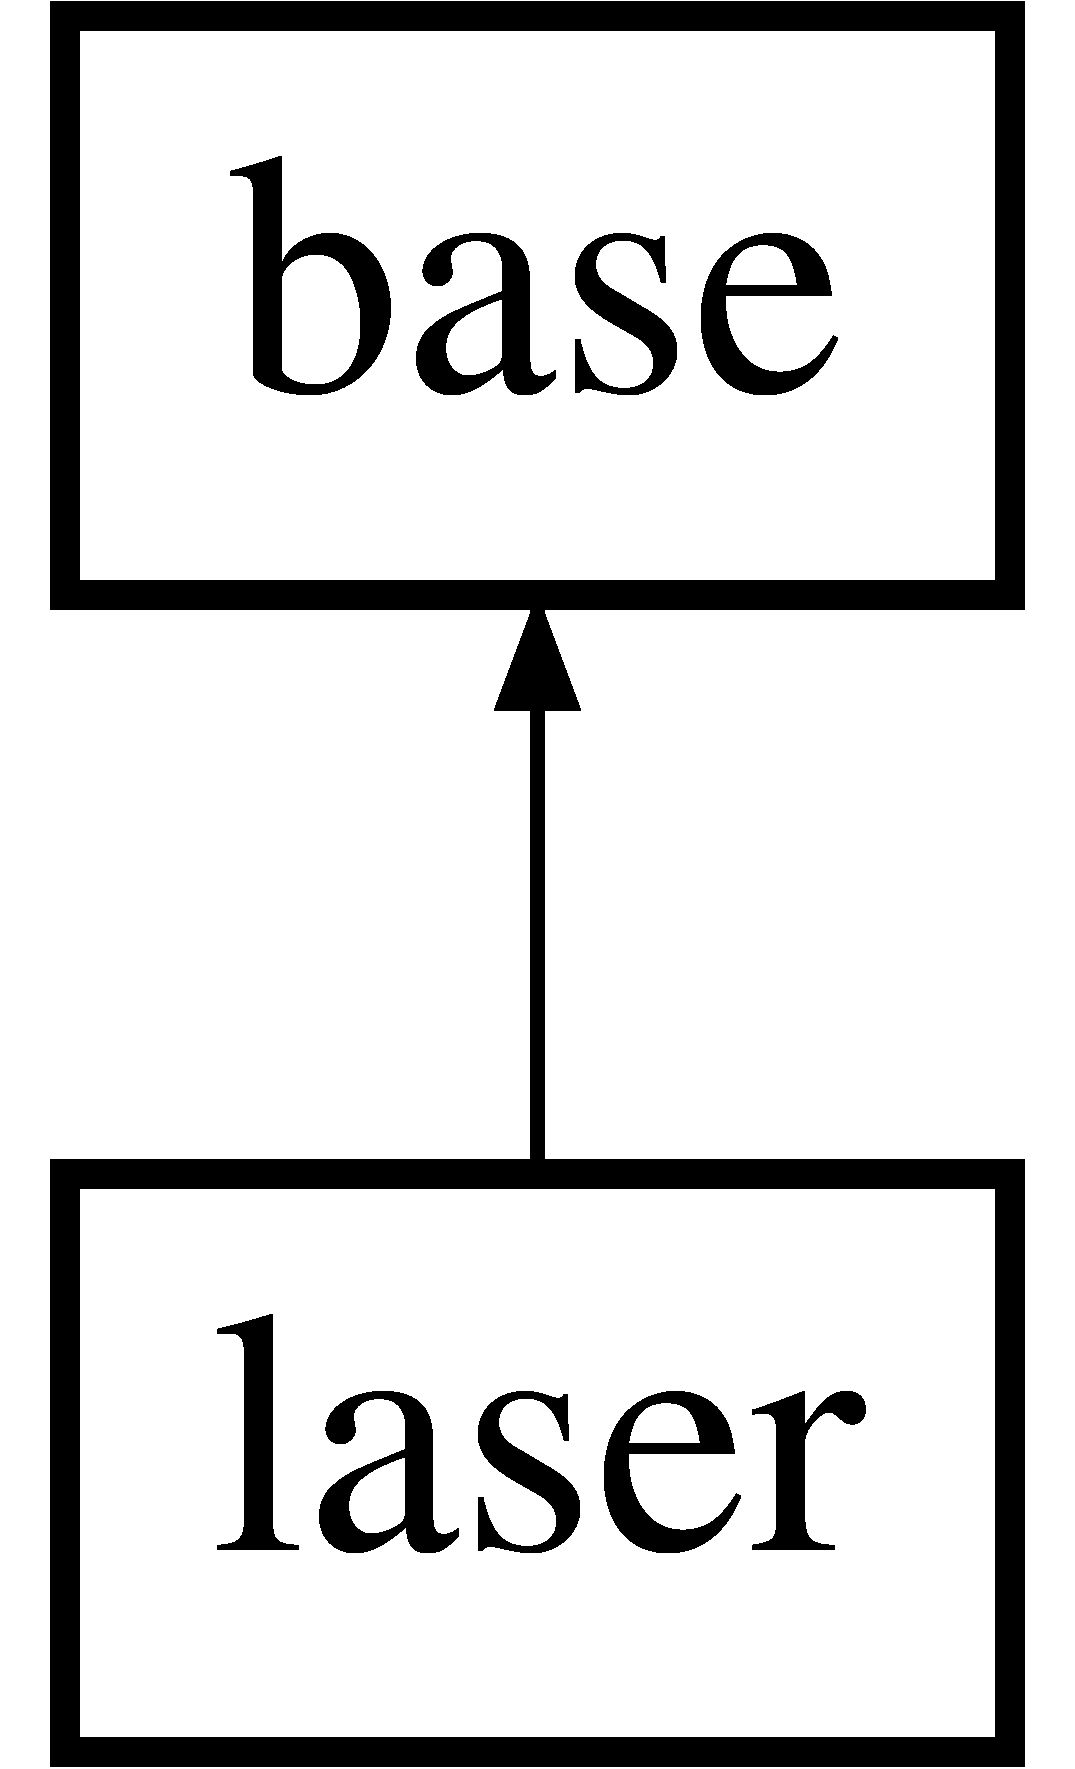
\includegraphics[height=2.000000cm]{classlaser}
\end{center}
\end{figure}
\subsection*{Public Member Functions}
\begin{DoxyCompactItemize}
\item 
\hyperlink{classlaser_a1abd02fb58a2910ced3e4f0a17abe5bd}{laser} (\hyperlink{structvec3}{vec3} \-\_\-p, \hyperlink{structvec3}{vec3} \-\_\-v, float \-\_\-ang, std\-::array$<$ float, W\-E\-A\-P\-S\-\_\-\-W $>$ \-\_\-data, \hyperlink{enemy_8hpp_abac1fdbabb5a6be5f0d6ae40be5c5a58}{ai\-Team} \-\_\-team)
\begin{DoxyCompactList}\small\item\em ctor for the laser class \end{DoxyCompactList}\item 
\hypertarget{classlaser_a56ca50fb28973ec2025acb23c838b946}{int \hyperlink{classlaser_a56ca50fb28973ec2025acb23c838b946}{get\-Dmg} () const }\label{classlaser_a56ca50fb28973ec2025acb23c838b946}

\begin{DoxyCompactList}\small\item\em returns damage \end{DoxyCompactList}\item 
\hypertarget{classlaser_ad3291de2cda3b474646f6bb4828b0593}{float \hyperlink{classlaser_ad3291de2cda3b474646f6bb4828b0593}{get\-Stop} () const }\label{classlaser_ad3291de2cda3b474646f6bb4828b0593}

\begin{DoxyCompactList}\small\item\em returns stopping power \end{DoxyCompactList}\item 
void \hyperlink{classlaser_a43ea4522e0aa950cb9aeaacc5555562c}{update} (float \-\_\-dt)
\begin{DoxyCompactList}\small\item\em updates the laser \end{DoxyCompactList}\item 
\hypertarget{classlaser_afcebdadf90172d4b3d9e5c98690cbd9d}{\hyperlink{enemy_8hpp_abac1fdbabb5a6be5f0d6ae40be5c5a58}{ai\-Team} \hyperlink{classlaser_afcebdadf90172d4b3d9e5c98690cbd9d}{get\-Team} () const }\label{classlaser_afcebdadf90172d4b3d9e5c98690cbd9d}

\begin{DoxyCompactList}\small\item\em returns the team \end{DoxyCompactList}\item 
\hypertarget{classlaser_a9f267e7172d09b4c8964e2b395de9564}{std\-::array$<$ float, 4 $>$ \hyperlink{classlaser_a9f267e7172d09b4c8964e2b395de9564}{get\-Col} () const }\label{classlaser_a9f267e7172d09b4c8964e2b395de9564}

\begin{DoxyCompactList}\small\item\em returns the colour of the laser. \end{DoxyCompactList}\item 
float \hyperlink{classlaser_a524a8e81d17a3dcf785268a3b1909bb4}{get\-Col} (int \-\_\-index) const 
\begin{DoxyCompactList}\small\item\em Getter for single colour component. \end{DoxyCompactList}\item 
\hypertarget{classlaser_a276c7f92329ac1cb3b47a2eb9ce647b1}{float \hyperlink{classlaser_a276c7f92329ac1cb3b47a2eb9ce647b1}{get\-Power} () const }\label{classlaser_a276c7f92329ac1cb3b47a2eb9ce647b1}

\begin{DoxyCompactList}\small\item\em Getter for laser power. \end{DoxyCompactList}\item 
\hypertarget{classlaser_a567fa22c33643684175934144c53fd6d}{float \hyperlink{classlaser_a567fa22c33643684175934144c53fd6d}{get\-Ang} () const }\label{classlaser_a567fa22c33643684175934144c53fd6d}

\begin{DoxyCompactList}\small\item\em Getter for the angle. \end{DoxyCompactList}\end{DoxyCompactItemize}


\subsection{Detailed Description}
Inherits from base, represents a laser and contains data such as faction, damage, colour etc. 

Inherits from ship, contains basic steering functionality. In some ways it is like a pared-\/down 'enemy' class. 

\subsection{Constructor \& Destructor Documentation}
\hypertarget{classlaser_a1abd02fb58a2910ced3e4f0a17abe5bd}{\index{laser@{laser}!laser@{laser}}
\index{laser@{laser}!laser@{laser}}
\subsubsection[{laser}]{\setlength{\rightskip}{0pt plus 5cm}laser\-::laser (
\begin{DoxyParamCaption}
\item[{{\bf vec3}}]{\-\_\-p, }
\item[{{\bf vec3}}]{\-\_\-v, }
\item[{float}]{\-\_\-ang, }
\item[{std\-::array$<$ float, W\-E\-A\-P\-S\-\_\-\-W $>$}]{\-\_\-data, }
\item[{{\bf ai\-Team}}]{\-\_\-team}
\end{DoxyParamCaption}
)}}\label{classlaser_a1abd02fb58a2910ced3e4f0a17abe5bd}


ctor for the laser class 


\begin{DoxyParams}{Parameters}
{\em \-\_\-p} & positio \\
\hline
{\em \-\_\-v} & velocity \\
\hline
{\em \-\_\-ang} & angle \\
\hline
{\em \-\_\-data} & copied from \hyperlink{weapons_8hpp}{weapons.\-hpp} \\
\hline
{\em \-\_\-team} & the lasers' team \\
\hline
\end{DoxyParams}


\subsection{Member Function Documentation}
\hypertarget{classlaser_a524a8e81d17a3dcf785268a3b1909bb4}{\index{laser@{laser}!get\-Col@{get\-Col}}
\index{get\-Col@{get\-Col}!laser@{laser}}
\subsubsection[{get\-Col}]{\setlength{\rightskip}{0pt plus 5cm}float laser\-::get\-Col (
\begin{DoxyParamCaption}
\item[{int}]{\-\_\-index}
\end{DoxyParamCaption}
) const\hspace{0.3cm}{\ttfamily [inline]}}}\label{classlaser_a524a8e81d17a3dcf785268a3b1909bb4}


Getter for single colour component. 


\begin{DoxyParams}{Parameters}
{\em \-\_\-index} & index of component to retrieve \\
\hline
\end{DoxyParams}
\hypertarget{classlaser_a43ea4522e0aa950cb9aeaacc5555562c}{\index{laser@{laser}!update@{update}}
\index{update@{update}!laser@{laser}}
\subsubsection[{update}]{\setlength{\rightskip}{0pt plus 5cm}void laser\-::update (
\begin{DoxyParamCaption}
\item[{float}]{\-\_\-dt}
\end{DoxyParamCaption}
)}}\label{classlaser_a43ea4522e0aa950cb9aeaacc5555562c}


updates the laser 


\begin{DoxyParams}{Parameters}
{\em \-\_\-dt} & time difference \\
\hline
\end{DoxyParams}


The documentation for this class was generated from the following files\-:\begin{DoxyCompactItemize}
\item 
include/\hyperlink{laser_8hpp}{laser.\-hpp}\item 
src/laser.\-cpp\end{DoxyCompactItemize}

\hypertarget{classmissile}{\section{missile Class Reference}
\label{classmissile}\index{missile@{missile}}
}
Inheritance diagram for missile\-:\begin{figure}[H]
\begin{center}
\leavevmode
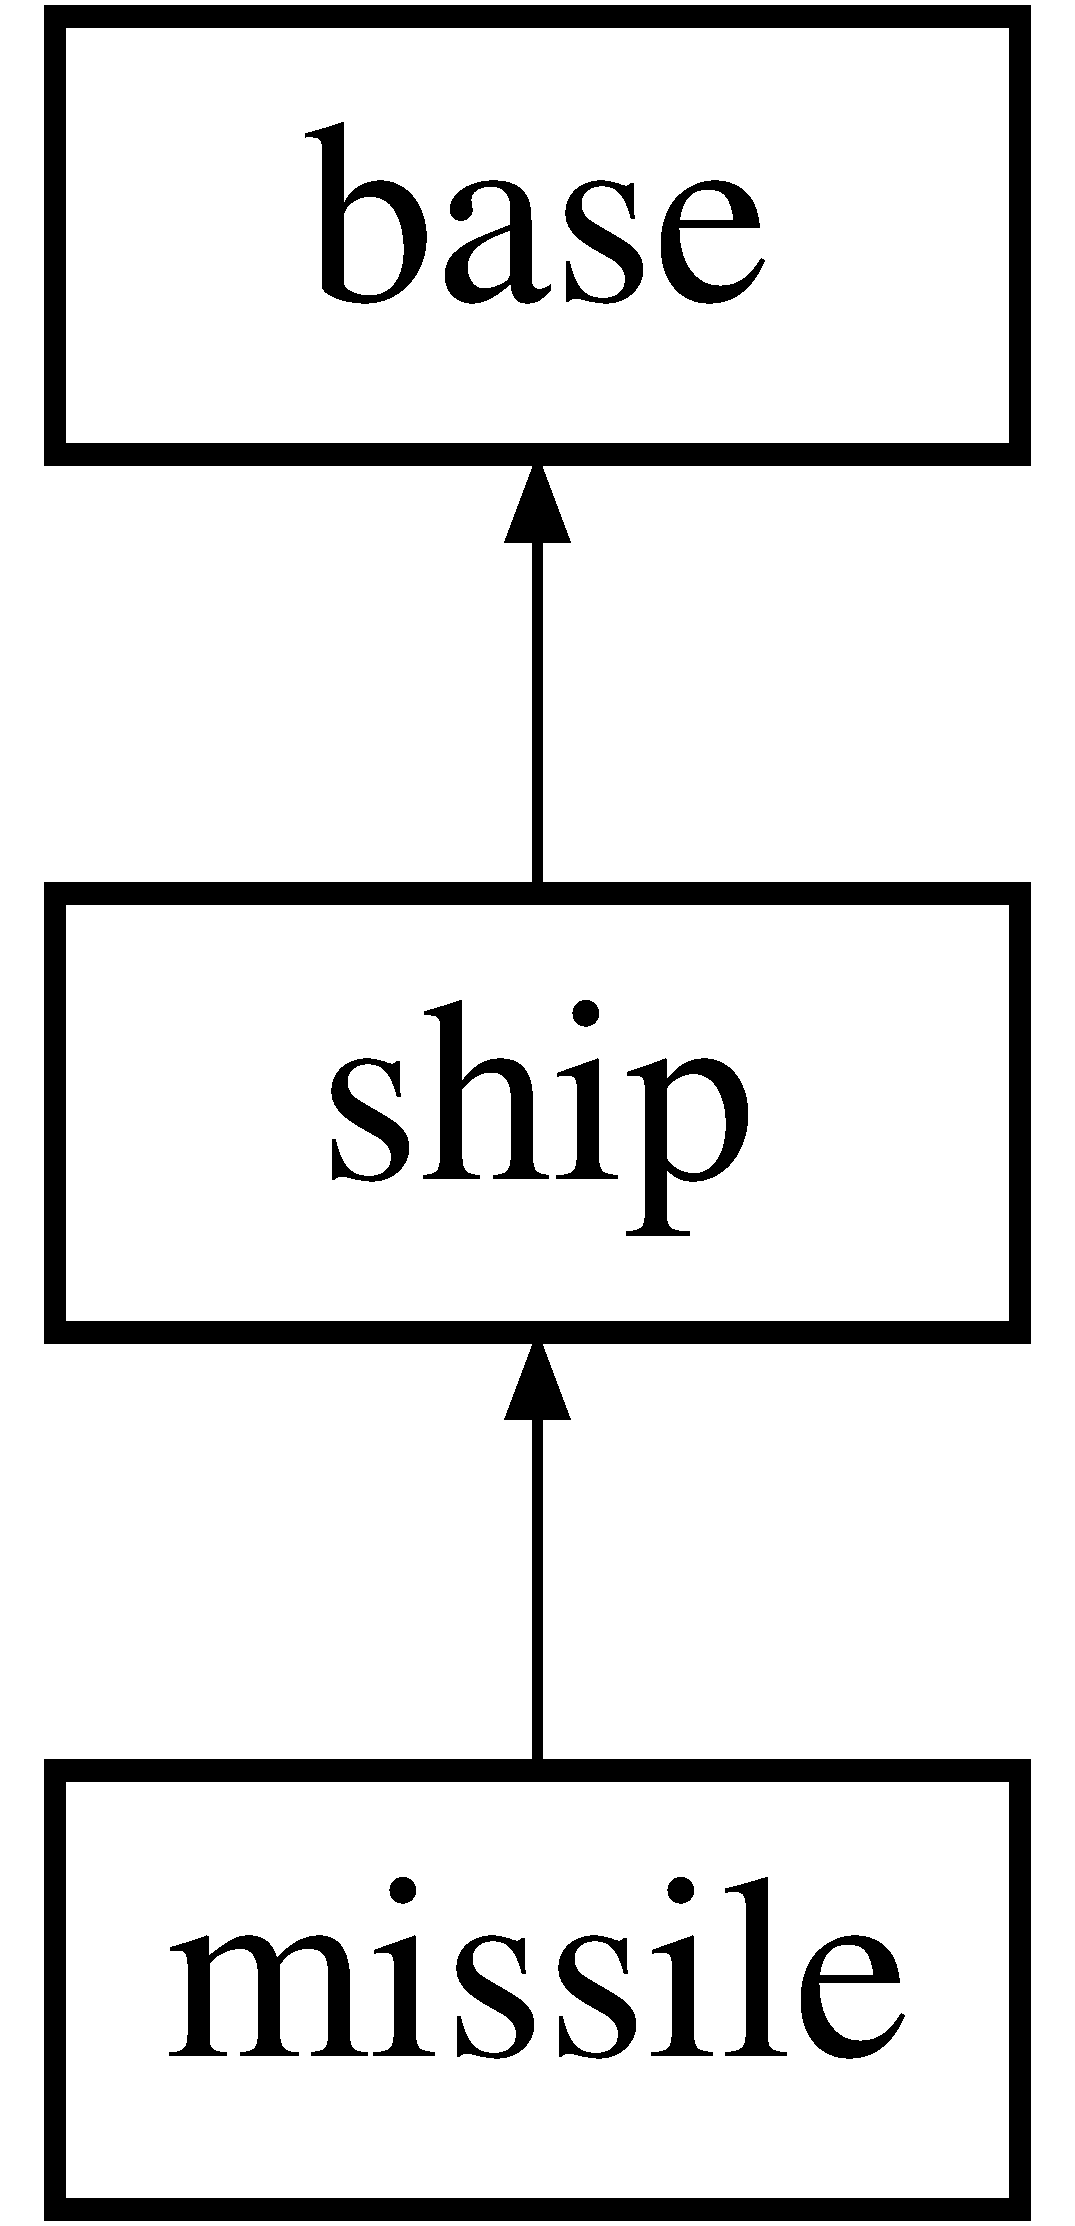
\includegraphics[height=3.000000cm]{classmissile}
\end{center}
\end{figure}
\subsection*{Public Member Functions}
\begin{DoxyCompactItemize}
\item 
\hyperlink{classmissile_a00f844af2c364c08cea07168947b709f}{missile} (const \hyperlink{structvec3}{vec3} \-\_\-p, const float \-\_\-r)
\begin{DoxyCompactList}\small\item\em ctor for the missile class \end{DoxyCompactList}\item 
void \hyperlink{classmissile_adb3b3adc21ee110967d2b5fbbd871e48}{set\-Target} (\hyperlink{classship}{ship} $\ast$\-\_\-s)
\begin{DoxyCompactList}\small\item\em sets the missiles' target \end{DoxyCompactList}\item 
\hypertarget{classmissile_acf40e8fe2ddfa4f028991e400ddd5003}{\hyperlink{classship}{ship} $\ast$ \hyperlink{classmissile_acf40e8fe2ddfa4f028991e400ddd5003}{get\-Target} () const }\label{classmissile_acf40e8fe2ddfa4f028991e400ddd5003}

\begin{DoxyCompactList}\small\item\em target getter \end{DoxyCompactList}\item 
\hypertarget{classmissile_a39c26b0f5a5946e9e3b484751e53c822}{void \hyperlink{classmissile_a39c26b0f5a5946e9e3b484751e53c822}{steering} ()}\label{classmissile_a39c26b0f5a5946e9e3b484751e53c822}

\begin{DoxyCompactList}\small\item\em steers the missile towards the target \end{DoxyCompactList}\item 
\hypertarget{classmissile_a8362636924cb31035ec0f09015d88e83}{bool \hyperlink{classmissile_a8362636924cb31035ec0f09015d88e83}{detonate} () const }\label{classmissile_a8362636924cb31035ec0f09015d88e83}

\begin{DoxyCompactList}\small\item\em m\-\_\-det getter \end{DoxyCompactList}\item 
\hypertarget{classmissile_a0443abaaeaed7e6ec0eca854eba06c60}{\hyperlink{enemy_8hpp_abac1fdbabb5a6be5f0d6ae40be5c5a58}{ai\-Team} \hyperlink{classmissile_a0443abaaeaed7e6ec0eca854eba06c60}{get\-Team} () const }\label{classmissile_a0443abaaeaed7e6ec0eca854eba06c60}

\begin{DoxyCompactList}\small\item\em team getter \end{DoxyCompactList}\end{DoxyCompactItemize}


\subsection{Constructor \& Destructor Documentation}
\hypertarget{classmissile_a00f844af2c364c08cea07168947b709f}{\index{missile@{missile}!missile@{missile}}
\index{missile@{missile}!missile@{missile}}
\subsubsection[{missile}]{\setlength{\rightskip}{0pt plus 5cm}missile\-::missile (
\begin{DoxyParamCaption}
\item[{const {\bf vec3}}]{\-\_\-p, }
\item[{const float}]{\-\_\-r}
\end{DoxyParamCaption}
)}}\label{classmissile_a00f844af2c364c08cea07168947b709f}


ctor for the missile class 


\begin{DoxyParams}{Parameters}
{\em \-\_\-p} & position \\
\hline
{\em \-\_\-r} & physical radius of the missile \\
\hline
\end{DoxyParams}


\subsection{Member Function Documentation}
\hypertarget{classmissile_adb3b3adc21ee110967d2b5fbbd871e48}{\index{missile@{missile}!set\-Target@{set\-Target}}
\index{set\-Target@{set\-Target}!missile@{missile}}
\subsubsection[{set\-Target}]{\setlength{\rightskip}{0pt plus 5cm}void missile\-::set\-Target (
\begin{DoxyParamCaption}
\item[{{\bf ship} $\ast$}]{\-\_\-s}
\end{DoxyParamCaption}
)\hspace{0.3cm}{\ttfamily [inline]}}}\label{classmissile_adb3b3adc21ee110967d2b5fbbd871e48}


sets the missiles' target 


\begin{DoxyParams}{Parameters}
{\em \-\_\-s} & the new target \\
\hline
\end{DoxyParams}


The documentation for this class was generated from the following files\-:\begin{DoxyCompactItemize}
\item 
include/\hyperlink{missile_8hpp}{missile.\-hpp}\item 
src/missile.\-cpp\end{DoxyCompactItemize}

\hypertarget{classpfx}{\section{pfx Class Reference}
\label{classpfx}\index{pfx@{pfx}}
}


Inherits from base, also contains instances of base.  




{\ttfamily \#include $<$pfx.\-hpp$>$}

Inheritance diagram for pfx\-:\begin{figure}[H]
\begin{center}
\leavevmode
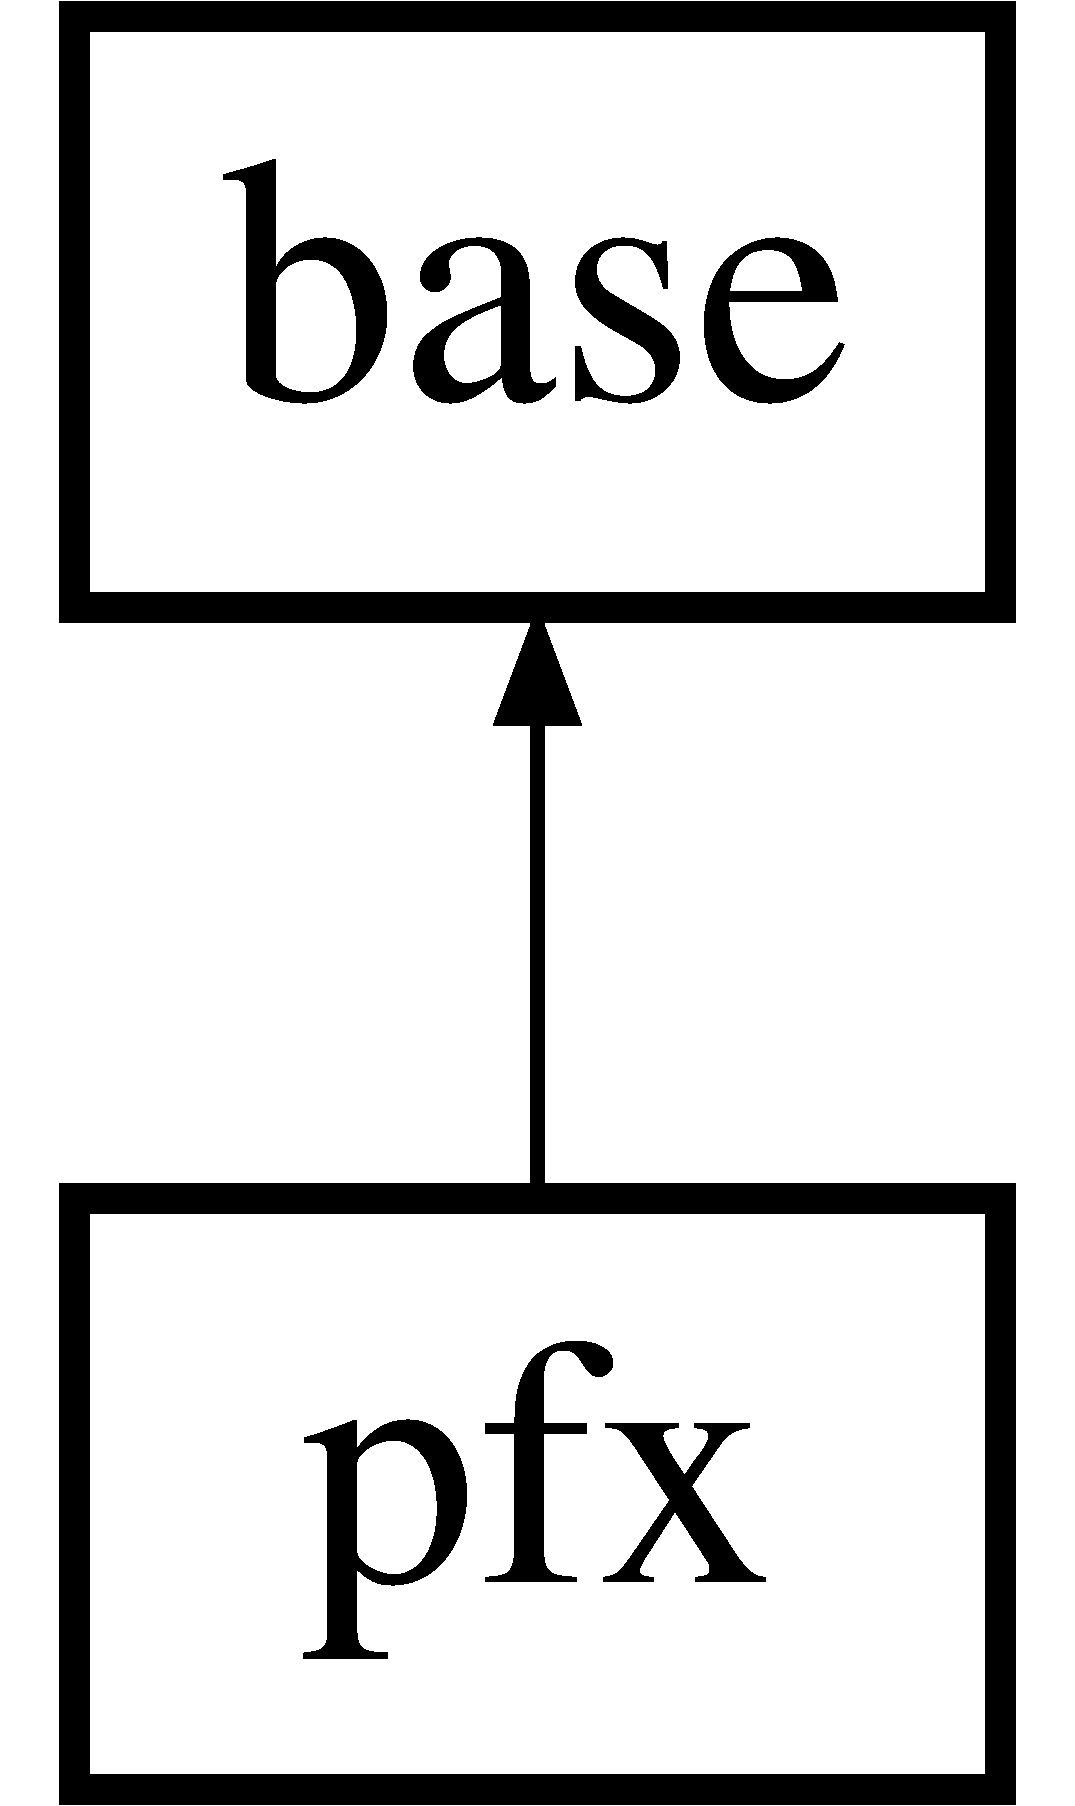
\includegraphics[height=2.000000cm]{classpfx}
\end{center}
\end{figure}
\subsection*{Public Member Functions}
\begin{DoxyCompactItemize}
\item 
\hyperlink{classpfx_ac84c5ea0b457660ae81912e4c9eed7fa}{pfx} (const \hyperlink{structvec3}{vec3} \-\_\-p, const \hyperlink{structvec3}{vec3} \-\_\-v, const \hyperlink{structvec3}{vec3} \-\_\-wv, const size\-\_\-t \-\_\-no, const float \-\_\-force, const std\-::string \-\_\-identifier)
\begin{DoxyCompactList}\small\item\em ctor for the pfx class \end{DoxyCompactList}\item 
void \hyperlink{classpfx_ac004ec0e3f4862aef0eab62a8c116663}{update} (float \-\_\-dt)
\begin{DoxyCompactList}\small\item\em Updates the system. \end{DoxyCompactList}\item 
\hypertarget{classpfx_a16585641dad66de325de7614bf66363a}{bool \hyperlink{classpfx_a16585641dad66de325de7614bf66363a}{done} () const }\label{classpfx_a16585641dad66de325de7614bf66363a}

\begin{DoxyCompactList}\small\item\em Has the effect finished? \end{DoxyCompactList}\item 
\hypertarget{classpfx_a224a96eb769197e7f389c691566f16d0}{std\-::array$<$ float, 3 $>$ \hyperlink{classpfx_a224a96eb769197e7f389c691566f16d0}{get\-Col} () const }\label{classpfx_a224a96eb769197e7f389c691566f16d0}

\begin{DoxyCompactList}\small\item\em Colour getters. \end{DoxyCompactList}\item 
\hypertarget{classpfx_a6d2cc538e428a1a8f4a1c6b95f574620}{float {\bfseries get\-Col} (int i) const }\label{classpfx_a6d2cc538e428a1a8f4a1c6b95f574620}

\item 
\hypertarget{classpfx_ab18819f5c1a18f748fe5cc00dbdcca59}{float \hyperlink{classpfx_ab18819f5c1a18f748fe5cc00dbdcca59}{get\-Alpha} () const }\label{classpfx_ab18819f5c1a18f748fe5cc00dbdcca59}

\begin{DoxyCompactList}\small\item\em Alpha getters. \end{DoxyCompactList}\item 
\hypertarget{classpfx_af2cdb7ea2176235eba7a3b4af8b05ed7}{float {\bfseries get\-Alpha} (const int index) const }\label{classpfx_af2cdb7ea2176235eba7a3b4af8b05ed7}

\item 
\hypertarget{classpfx_aaa8626d7c9ec5d701fd4d953333f3473}{std\-::string \hyperlink{classpfx_aaa8626d7c9ec5d701fd4d953333f3473}{get\-Identifier} () const }\label{classpfx_aaa8626d7c9ec5d701fd4d953333f3473}

\begin{DoxyCompactList}\small\item\em Identifier getter. \end{DoxyCompactList}\item 
\hypertarget{classpfx_a2bd03654be340d4c43bb51e01c666b8a}{std\-::vector$<$ \hyperlink{classbase}{base} $>$ $\ast$ \hyperlink{classpfx_a2bd03654be340d4c43bb51e01c666b8a}{get\-Particles} ()}\label{classpfx_a2bd03654be340d4c43bb51e01c666b8a}

\begin{DoxyCompactList}\small\item\em Returns the child particle vector. \end{DoxyCompactList}\item 
\hypertarget{classpfx_a0744ef49ef96b16fa25ec417b59388c4}{float \hyperlink{classpfx_a0744ef49ef96b16fa25ec417b59388c4}{get\-Force} ()}\label{classpfx_a0744ef49ef96b16fa25ec417b59388c4}

\begin{DoxyCompactList}\small\item\em Force getter. \end{DoxyCompactList}\end{DoxyCompactItemize}


\subsection{Detailed Description}
Inherits from base, also contains instances of base. 

\subsection{Constructor \& Destructor Documentation}
\hypertarget{classpfx_ac84c5ea0b457660ae81912e4c9eed7fa}{\index{pfx@{pfx}!pfx@{pfx}}
\index{pfx@{pfx}!pfx@{pfx}}
\subsubsection[{pfx}]{\setlength{\rightskip}{0pt plus 5cm}pfx\-::pfx (
\begin{DoxyParamCaption}
\item[{const {\bf vec3}}]{\-\_\-p, }
\item[{const {\bf vec3}}]{\-\_\-v, }
\item[{const {\bf vec3}}]{\-\_\-wv, }
\item[{const size\-\_\-t}]{\-\_\-no, }
\item[{const float}]{\-\_\-force, }
\item[{const std\-::string}]{\-\_\-identifier}
\end{DoxyParamCaption}
)}}\label{classpfx_ac84c5ea0b457660ae81912e4c9eed7fa}


ctor for the pfx class 


\begin{DoxyParams}{Parameters}
{\em \-\_\-p} & position \\
\hline
{\em \-\_\-v} & center velocit y \\
\hline
{\em \-\_\-no} & number of children \\
\hline
{\em \-\_\-force} & velocity multiplier of children \\
\hline
{\em \-\_\-identifier} & type of effect, such as \char`\"{}\-S\-M\-O\-K\-E\char`\"{}, \char`\"{}\-E\-X\-P\-L\-O\-S\-I\-O\-N\char`\"{} etc \\
\hline
\end{DoxyParams}


\subsection{Member Function Documentation}
\hypertarget{classpfx_ac004ec0e3f4862aef0eab62a8c116663}{\index{pfx@{pfx}!update@{update}}
\index{update@{update}!pfx@{pfx}}
\subsubsection[{update}]{\setlength{\rightskip}{0pt plus 5cm}void pfx\-::update (
\begin{DoxyParamCaption}
\item[{float}]{\-\_\-dt}
\end{DoxyParamCaption}
)}}\label{classpfx_ac004ec0e3f4862aef0eab62a8c116663}


Updates the system. 


\begin{DoxyParams}{Parameters}
{\em \-\_\-dt} & Time difference \\
\hline
\end{DoxyParams}


The documentation for this class was generated from the following files\-:\begin{DoxyCompactItemize}
\item 
include/\hyperlink{pfx_8hpp}{pfx.\-hpp}\item 
src/pfx.\-cpp\end{DoxyCompactItemize}

\hypertarget{classplayer}{\section{player Class Reference}
\label{classplayer}\index{player@{player}}
}


Builds upon the ship class, but unlike the enemy class adds controls rather than A\-I.  




{\ttfamily \#include $<$player.\-hpp$>$}

Inheritance diagram for player\-:\begin{figure}[H]
\begin{center}
\leavevmode
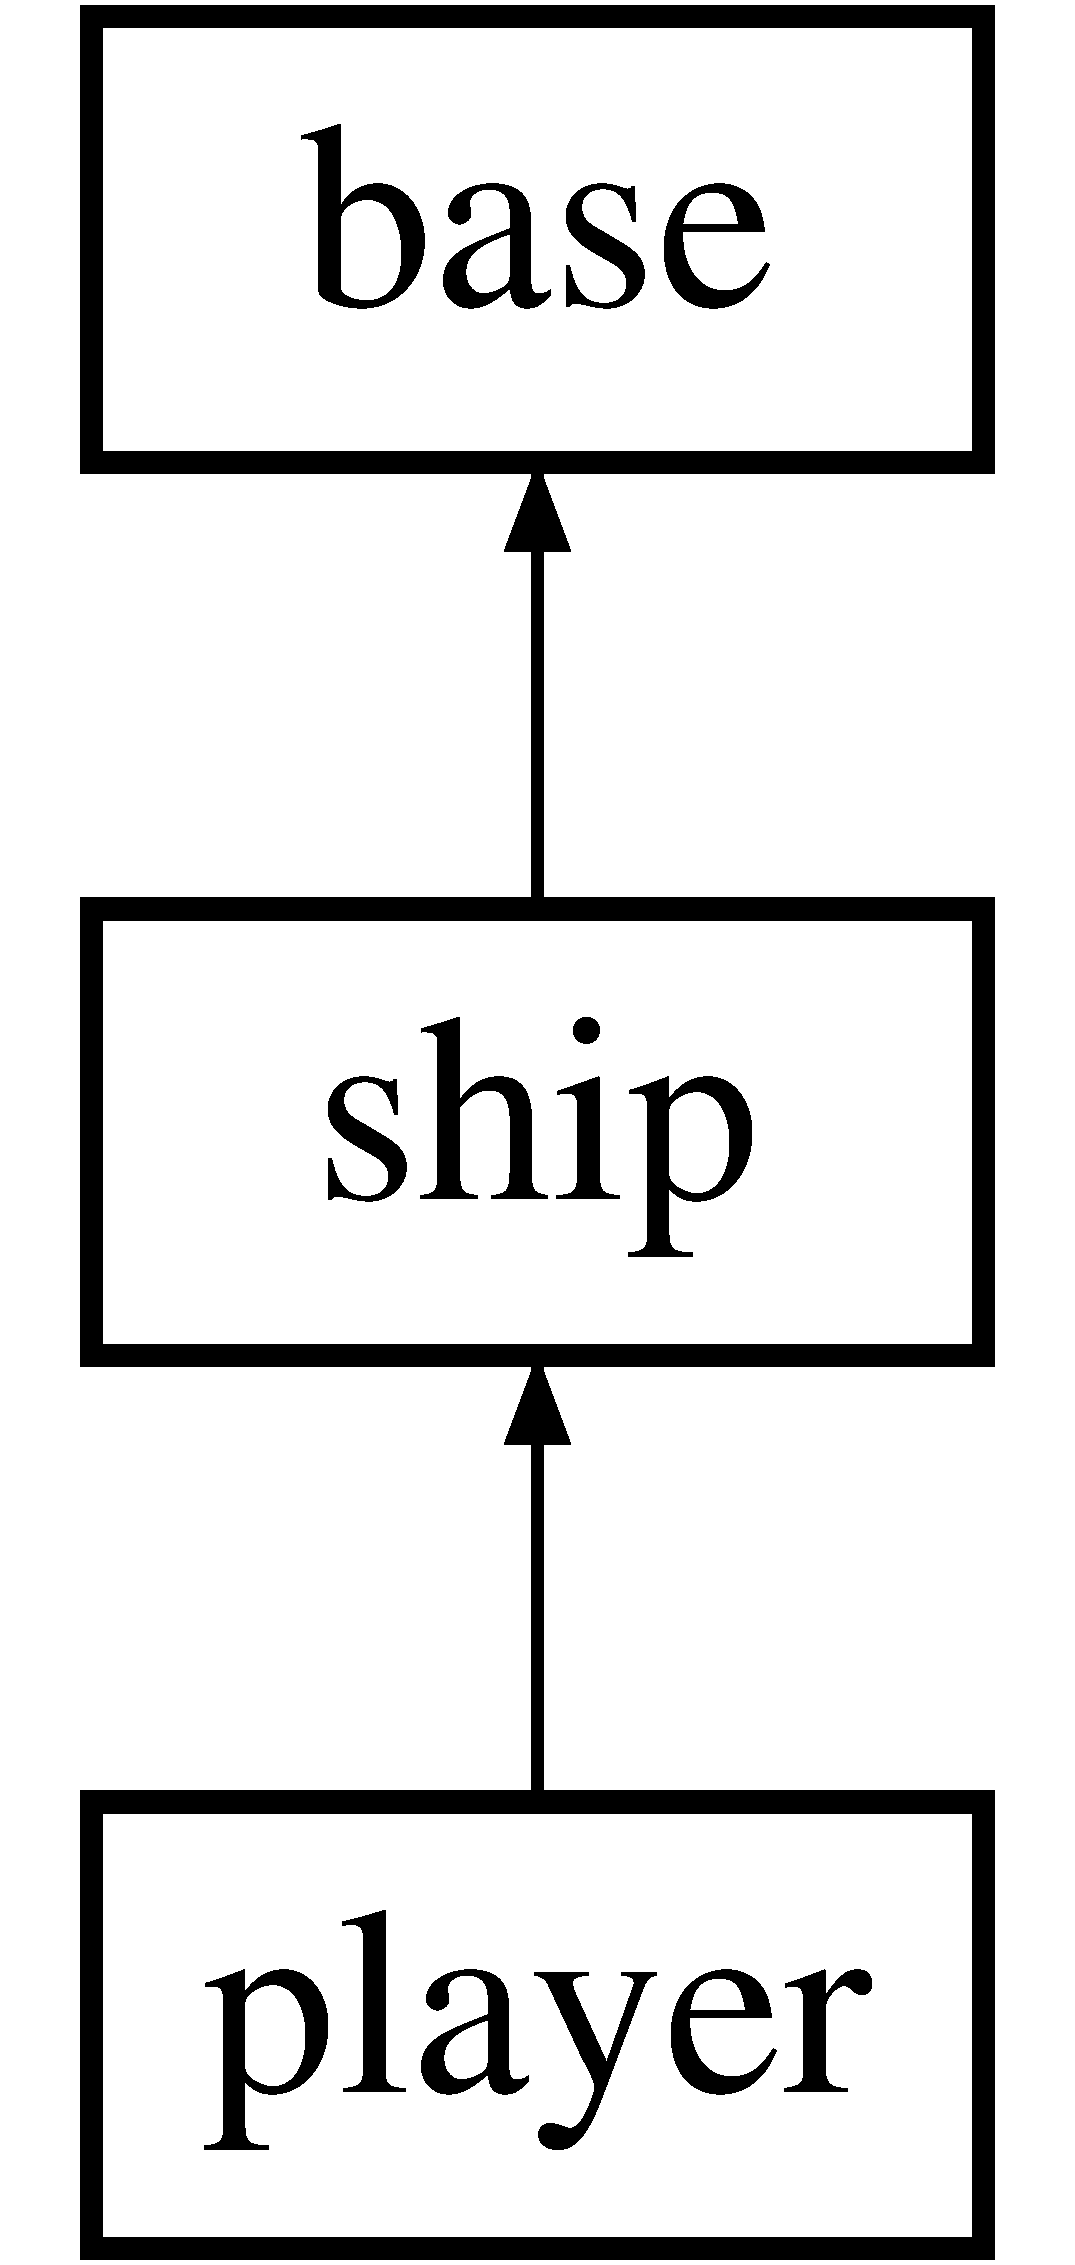
\includegraphics[height=3.000000cm]{classplayer}
\end{center}
\end{figure}
\subsection*{Public Member Functions}
\begin{DoxyCompactItemize}
\item 
\hyperlink{classplayer_a9b375359a880c6fe0294ffd11d498761}{player} (\hyperlink{structvec3}{vec3} \-\_\-p, float \-\_\-r)
\begin{DoxyCompactList}\small\item\em ctor for the player \end{DoxyCompactList}\item 
\hypertarget{classplayer_a232e4cb06a429758f6acec8d16c71b08}{void \hyperlink{classplayer_a232e4cb06a429758f6acec8d16c71b08}{ctrl\-Update} ()}\label{classplayer_a232e4cb06a429758f6acec8d16c71b08}

\begin{DoxyCompactList}\small\item\em Updates the player, processes some user input. \end{DoxyCompactList}\end{DoxyCompactItemize}


\subsection{Detailed Description}
Builds upon the ship class, but unlike the enemy class adds controls rather than A\-I. 

\subsection{Constructor \& Destructor Documentation}
\hypertarget{classplayer_a9b375359a880c6fe0294ffd11d498761}{\index{player@{player}!player@{player}}
\index{player@{player}!player@{player}}
\subsubsection[{player}]{\setlength{\rightskip}{0pt plus 5cm}player\-::player (
\begin{DoxyParamCaption}
\item[{{\bf vec3}}]{\-\_\-p, }
\item[{float}]{\-\_\-r}
\end{DoxyParamCaption}
)}}\label{classplayer_a9b375359a880c6fe0294ffd11d498761}


ctor for the player 


\begin{DoxyParams}{Parameters}
{\em \-\_\-p} & position \\
\hline
{\em \-\_\-r} & ship radius \\
\hline
\end{DoxyParams}


The documentation for this class was generated from the following files\-:\begin{DoxyCompactItemize}
\item 
include/\hyperlink{player_8hpp}{player.\-hpp}\item 
src/player.\-cpp\end{DoxyCompactItemize}

\hypertarget{classrenderer}{\section{renderer Class Reference}
\label{classrenderer}\index{renderer@{renderer}}
}


Wrapper around S\-D\-L rendering functionality. Has not been updated in a bit, use at your own risk.  




{\ttfamily \#include $<$renderer.\-hpp$>$}

\subsection*{Public Member Functions}
\begin{DoxyCompactItemize}
\item 
\hyperlink{classrenderer_ab24dfda8eda699409c6f64eaa3d3d681}{renderer} (int \-\_\-w, int \-\_\-h)
\begin{DoxyCompactList}\small\item\em ctor for the renderer \end{DoxyCompactList}\item 
\hypertarget{classrenderer_a5c7f1cfc1cd1292c2ec8519dacdce0a6}{\hyperlink{classrenderer_a5c7f1cfc1cd1292c2ec8519dacdce0a6}{$\sim$renderer} ()}\label{classrenderer_a5c7f1cfc1cd1292c2ec8519dacdce0a6}

\begin{DoxyCompactList}\small\item\em dtor for the renderer, frees up memory tied to all the dynamically allocated S\-D\-L objects \end{DoxyCompactList}\item 
\hypertarget{classrenderer_a92f72123ee07357e08173e8eea641ad4}{int \hyperlink{classrenderer_a92f72123ee07357e08173e8eea641ad4}{init} ()}\label{classrenderer_a92f72123ee07357e08173e8eea641ad4}

\begin{DoxyCompactList}\small\item\em Initialises essential S\-D\-L functionality. \end{DoxyCompactList}\item 
\hypertarget{classrenderer_a025d4becc60b9ef886b7f0fee06d015a}{void \hyperlink{classrenderer_a025d4becc60b9ef886b7f0fee06d015a}{load\-Textures} ()}\label{classrenderer_a025d4becc60b9ef886b7f0fee06d015a}

\begin{DoxyCompactList}\small\item\em Loads all of the required textures. \end{DoxyCompactList}\item 
void \hyperlink{classrenderer_ad06ba9c15401bb0dcdafb525cfd8f201}{update} (const float \-\_\-dt)
\begin{DoxyCompactList}\small\item\em Updates the renderer, mostly used to update camera shake. \end{DoxyCompactList}\item 
void \hyperlink{classrenderer_abab0176fc41988510f7602da75e885fc}{load\-Font\-Sprite\-Sheet} (std\-::string \-\_\-name, std\-::string \-\_\-path, int \-\_\-size)
\begin{DoxyCompactList}\small\item\em Loads glyphs from a font and renders them to S\-D\-L textures. \end{DoxyCompactList}\item 
void \hyperlink{classrenderer_a56924d177465861dc6273e6ff5de220d}{load\-Texture} (std\-::string \-\_\-key, std\-::string \-\_\-path, S\-D\-L\-\_\-\-Blend\-Mode \-\_\-b)
\begin{DoxyCompactList}\small\item\em Loads an image and stores it as an S\-D\-L texture. \end{DoxyCompactList}\item 
void \hyperlink{classrenderer_acc26e337a27867cfc52193774986ff7c}{load\-Texture\-Set} (std\-::string \-\_\-key, std\-::string \-\_\-set)
\begin{DoxyCompactList}\small\item\em Loads a set of images, converts them to textures, and stores them. \end{DoxyCompactList}\item 
void \hyperlink{classrenderer_a9355f220b4ea6a7a528913b6878bded2}{set\-Blend\-Mode} (S\-D\-L\-\_\-\-Blend\-Mode \-\_\-b)
\begin{DoxyCompactList}\small\item\em Loads a set of images, converts them to textures, and stores them. \end{DoxyCompactList}\item 
\hypertarget{classrenderer_aab9e421ec4b4fa5a1ce6ebe4dfa9b22c}{void \hyperlink{classrenderer_aab9e421ec4b4fa5a1ce6ebe4dfa9b22c}{clear} ()}\label{classrenderer_aab9e421ec4b4fa5a1ce6ebe4dfa9b22c}

\begin{DoxyCompactList}\small\item\em Clears the screen. \end{DoxyCompactList}\item 
void \hyperlink{classrenderer_aff2e7ad5dc4d7b8b26e496b5baa5a8de}{draw\-Texture\-Set} (std\-::string \-\_\-key, \hyperlink{structvec2}{vec2} \-\_\-pos, float \-\_\-orient, std\-::array$<$ float, 4 $>$ \-\_\-col)
\begin{DoxyCompactList}\small\item\em Draws a set of textures to the screen, used for objects like ships, which have multiple components. \end{DoxyCompactList}\item 
void \hyperlink{classrenderer_a6afff3128edc0e0caab88d51a1de022b}{draw\-Texture} (std\-::string \-\_\-key, size\-\_\-t \-\_\-index, \hyperlink{structvec2}{vec2} \-\_\-pos, float \-\_\-orient, std\-::array$<$ float, 4 $>$ \-\_\-col)
\begin{DoxyCompactList}\small\item\em Draws a texture to the screen. \end{DoxyCompactList}\item 
void \hyperlink{classrenderer_a430af103157a244d083c16b41a6b839b}{draw\-Text} (std\-::string \-\_\-text, std\-::string \-\_\-font, \hyperlink{structvec2}{vec2} \-\_\-pos, bool \-\_\-ss, const float \-\_\-mul)
\begin{DoxyCompactList}\small\item\em Draws text to the screen. \end{DoxyCompactList}\item 
void \hyperlink{classrenderer_a7c6f70612d8fc6e6c1d9520c73e81f94}{draw\-Line} (\hyperlink{structvec2}{vec2} \-\_\-start, \hyperlink{structvec2}{vec2} \-\_\-end, std\-::array$<$ float, 4 $>$ \-\_\-col)
\begin{DoxyCompactList}\small\item\em \hyperlink{struct_a}{A} wrapper around S\-D\-L's line drawing function, draws a coloured line. \end{DoxyCompactList}\item 
\hypertarget{classrenderer_a0a19a18380a5b0155a0741bc9cf5f1d5}{void {\bfseries draw\-Line} (\hyperlink{structvec2}{vec2} \-\_\-start, \hyperlink{structvec2}{vec2} \-\_\-end, std\-::array$<$ int, 4 $>$ \-\_\-col)}\label{classrenderer_a0a19a18380a5b0155a0741bc9cf5f1d5}

\item 
void \hyperlink{classrenderer_a3564517ce29f05e45b881a4c8afa3f96}{draw\-Line\-Gr} (\hyperlink{structvec2}{vec2} \-\_\-p, \hyperlink{structvec2}{vec2} \-\_\-e, std\-::array$<$ float, 4 $>$ \-\_\-scol, std\-::array$<$ float, 4 $>$ \-\_\-ecol)
\begin{DoxyCompactList}\small\item\em Draws line whose colour varies. \end{DoxyCompactList}\item 
void \hyperlink{classrenderer_afc96317d24e4c0210053dffc0d191d6e}{draw\-Rect} (\hyperlink{structvec2}{vec2} \-\_\-p, \hyperlink{structvec2}{vec2} \-\_\-d, std\-::array$<$ int, 4 $>$ col, bool \-\_\-wire)
\begin{DoxyCompactList}\small\item\em Draws a rectangle. \end{DoxyCompactList}\item 
void \hyperlink{classrenderer_a575e3c10997f1fe8ec941dfa1e4efd01}{draw\-Circle} (int \-\_\-x, int \-\_\-y, int \-\_\-radius, std\-::array$<$ float, 4 $>$ \-\_\-col)
\begin{DoxyCompactList}\small\item\em Draws a circle. \end{DoxyCompactList}\item 
\hypertarget{classrenderer_a93e0d322c1bace835ccf19f3f6bc184d}{void {\bfseries draw\-Circle\-U\-I} (int \-\_\-x, int \-\_\-y, int \-\_\-radius, std\-::array$<$ int, 4 $>$ \-\_\-col)}\label{classrenderer_a93e0d322c1bace835ccf19f3f6bc184d}

\item 
void \hyperlink{classrenderer_a70a52c25aab83762d2e6a9e89a7e3f68}{query\-Texture} (std\-::string \-\_\-identifier, int \-\_\-index, int $\ast$\-\_\-w, int $\ast$\-\_\-h)
\begin{DoxyCompactList}\small\item\em Returns the dimensions of a texture. \end{DoxyCompactList}\item 
float \hyperlink{classrenderer_a560b721679d96689a77155fb4d2bf36a}{get\-Texture\-Radius} (\hyperlink{ship_8hpp_af74a63841701826d661cb9809aaf7092}{ship\-\_\-spec} \-\_\-type)
\begin{DoxyCompactList}\small\item\em Returns the radius of the texture of a ship type. \end{DoxyCompactList}\item 
void \hyperlink{classrenderer_a705585261bc8aeca559e96cfe558712e}{draw\-Map} (std\-::vector$<$ \hyperlink{classmissile}{missile} $>$ $\ast$\-\_\-mp, std\-::vector$<$ \hyperlink{classenemy}{enemy} $>$ $\ast$\-\_\-ep, std\-::vector$<$ \hyperlink{classship}{ship} $>$ $\ast$\-\_\-ap, std\-::vector$<$ \hyperlink{classlaser}{laser} $>$ $\ast$\-\_\-lp, std\-::vector$<$ \hyperlink{structfaction}{faction} $>$ $\ast$\-\_\-fp)
\begin{DoxyCompactList}\small\item\em Draws the minimap. \end{DoxyCompactList}\item 
void \hyperlink{classrenderer_a78e5ab3b46c708c369fddeac1202c692}{status\-Bars} (\hyperlink{classplayer}{player} $\ast$\-\_\-ply)
\begin{DoxyCompactList}\small\item\em Draws health, shield and energy bars. \end{DoxyCompactList}\item 
void \hyperlink{classrenderer_a0e00b3fbe340e2f152856bd3686b563a}{draw\-Weapon\-Stats} (\hyperlink{classplayer}{player} $\ast$\-\_\-ply)
\begin{DoxyCompactList}\small\item\em Draw the stats of the current weapon. \end{DoxyCompactList}\item 
\hypertarget{classrenderer_ae42befa84c772f9a79624411dc31a7dc}{void \hyperlink{classrenderer_ae42befa84c772f9a79624411dc31a7dc}{finalise} ()}\label{classrenderer_ae42befa84c772f9a79624411dc31a7dc}

\begin{DoxyCompactList}\small\item\em Displays the contents of the renderer. \end{DoxyCompactList}\item 
S\-D\-L\-\_\-\-Surface $\ast$ \hyperlink{classrenderer_a89fa8841ece29c81878f31f5aa02132c}{get\-Surface} (std\-::string \-\_\-path)
\begin{DoxyCompactList}\small\item\em Loads an image as an S\-D\-L Surface, and returns a pointer to it. \end{DoxyCompactList}\item 
void \hyperlink{classrenderer_ac0fe40b19aa7e976a7c84b6a12318235}{add\-Shake} (float \-\_\-s)
\begin{DoxyCompactList}\small\item\em Adds screen shake. \end{DoxyCompactList}\item 
void \hyperlink{classrenderer_a7502c6754f0dec9b8324c154b10557ce}{to\-Octant} (int $\ast$\-\_\-x, int $\ast$\-\_\-y, int \-\_\-octant)
\begin{DoxyCompactList}\small\item\em Used to draw circles, converts a pair of coordinates to a specified octant. \end{DoxyCompactList}\end{DoxyCompactItemize}


\subsection{Detailed Description}
Wrapper around S\-D\-L rendering functionality. Has not been updated in a bit, use at your own risk. 

\subsection{Constructor \& Destructor Documentation}
\hypertarget{classrenderer_ab24dfda8eda699409c6f64eaa3d3d681}{\index{renderer@{renderer}!renderer@{renderer}}
\index{renderer@{renderer}!renderer@{renderer}}
\subsubsection[{renderer}]{\setlength{\rightskip}{0pt plus 5cm}renderer\-::renderer (
\begin{DoxyParamCaption}
\item[{int}]{\-\_\-w, }
\item[{int}]{\-\_\-h}
\end{DoxyParamCaption}
)}}\label{classrenderer_ab24dfda8eda699409c6f64eaa3d3d681}


ctor for the renderer 


\begin{DoxyParams}{Parameters}
{\em \-\_\-w} & window width \\
\hline
{\em \-\_\-h} & window height \\
\hline
\end{DoxyParams}


\subsection{Member Function Documentation}
\hypertarget{classrenderer_ac0fe40b19aa7e976a7c84b6a12318235}{\index{renderer@{renderer}!add\-Shake@{add\-Shake}}
\index{add\-Shake@{add\-Shake}!renderer@{renderer}}
\subsubsection[{add\-Shake}]{\setlength{\rightskip}{0pt plus 5cm}void renderer\-::add\-Shake (
\begin{DoxyParamCaption}
\item[{float}]{\-\_\-s}
\end{DoxyParamCaption}
)}}\label{classrenderer_ac0fe40b19aa7e976a7c84b6a12318235}


Adds screen shake. 


\begin{DoxyParams}{Parameters}
{\em \-\_\-s} & magnitude \\
\hline
\end{DoxyParams}
\hypertarget{classrenderer_a575e3c10997f1fe8ec941dfa1e4efd01}{\index{renderer@{renderer}!draw\-Circle@{draw\-Circle}}
\index{draw\-Circle@{draw\-Circle}!renderer@{renderer}}
\subsubsection[{draw\-Circle}]{\setlength{\rightskip}{0pt plus 5cm}void renderer\-::draw\-Circle (
\begin{DoxyParamCaption}
\item[{int}]{\-\_\-x, }
\item[{int}]{\-\_\-y, }
\item[{int}]{\-\_\-radius, }
\item[{std\-::array$<$ float, 4 $>$}]{\-\_\-col}
\end{DoxyParamCaption}
)}}\label{classrenderer_a575e3c10997f1fe8ec941dfa1e4efd01}


Draws a circle. 


\begin{DoxyParams}{Parameters}
{\em \-\_\-x} & x-\/coord \\
\hline
{\em \-\_\-y} & y-\/coord \\
\hline
{\em \-\_\-radius} & circle radius \\
\hline
{\em \-\_\-col} & circle colour \\
\hline
\end{DoxyParams}
\hypertarget{classrenderer_a7c6f70612d8fc6e6c1d9520c73e81f94}{\index{renderer@{renderer}!draw\-Line@{draw\-Line}}
\index{draw\-Line@{draw\-Line}!renderer@{renderer}}
\subsubsection[{draw\-Line}]{\setlength{\rightskip}{0pt plus 5cm}void renderer\-::draw\-Line (
\begin{DoxyParamCaption}
\item[{{\bf vec2}}]{\-\_\-start, }
\item[{{\bf vec2}}]{\-\_\-end, }
\item[{std\-::array$<$ float, 4 $>$}]{\-\_\-col}
\end{DoxyParamCaption}
)}}\label{classrenderer_a7c6f70612d8fc6e6c1d9520c73e81f94}


\hyperlink{struct_a}{A} wrapper around S\-D\-L's line drawing function, draws a coloured line. 


\begin{DoxyParams}{Parameters}
{\em \-\_\-start} & start position \\
\hline
{\em \-\_\-end} & end position \\
\hline
{\em \-\_\-col} & line colour \\
\hline
\end{DoxyParams}
\hypertarget{classrenderer_a3564517ce29f05e45b881a4c8afa3f96}{\index{renderer@{renderer}!draw\-Line\-Gr@{draw\-Line\-Gr}}
\index{draw\-Line\-Gr@{draw\-Line\-Gr}!renderer@{renderer}}
\subsubsection[{draw\-Line\-Gr}]{\setlength{\rightskip}{0pt plus 5cm}void renderer\-::draw\-Line\-Gr (
\begin{DoxyParamCaption}
\item[{{\bf vec2}}]{\-\_\-p, }
\item[{{\bf vec2}}]{\-\_\-e, }
\item[{std\-::array$<$ float, 4 $>$}]{\-\_\-scol, }
\item[{std\-::array$<$ float, 4 $>$}]{\-\_\-ecol}
\end{DoxyParamCaption}
)}}\label{classrenderer_a3564517ce29f05e45b881a4c8afa3f96}


Draws line whose colour varies. 


\begin{DoxyParams}{Parameters}
{\em \-\_\-p} & line start \\
\hline
{\em \-\_\-e} & line end \\
\hline
{\em \-\_\-scol} & start colour \\
\hline
{\em \-\_\-ecol} & end colour \\
\hline
\end{DoxyParams}
\hypertarget{classrenderer_a705585261bc8aeca559e96cfe558712e}{\index{renderer@{renderer}!draw\-Map@{draw\-Map}}
\index{draw\-Map@{draw\-Map}!renderer@{renderer}}
\subsubsection[{draw\-Map}]{\setlength{\rightskip}{0pt plus 5cm}void renderer\-::draw\-Map (
\begin{DoxyParamCaption}
\item[{std\-::vector$<$ {\bf missile} $>$ $\ast$}]{\-\_\-mp, }
\item[{std\-::vector$<$ {\bf enemy} $>$ $\ast$}]{\-\_\-ep, }
\item[{std\-::vector$<$ {\bf ship} $>$ $\ast$}]{\-\_\-ap, }
\item[{std\-::vector$<$ {\bf laser} $>$ $\ast$}]{\-\_\-lp, }
\item[{std\-::vector$<$ {\bf faction} $>$ $\ast$}]{\-\_\-fp}
\end{DoxyParamCaption}
)}}\label{classrenderer_a705585261bc8aeca559e96cfe558712e}


Draws the minimap. 


\begin{DoxyParams}{Parameters}
{\em \-\_\-mp} & ref to missile vector \\
\hline
{\em \-\_\-ep} & ref to agent vector \\
\hline
{\em \-\_\-ap} & ref to asteroid vector \\
\hline
{\em \-\_\-lp} & ref to laser vector \\
\hline
{\em \-\_\-fp} & ref to faction pointer \\
\hline
\end{DoxyParams}
\hypertarget{classrenderer_afc96317d24e4c0210053dffc0d191d6e}{\index{renderer@{renderer}!draw\-Rect@{draw\-Rect}}
\index{draw\-Rect@{draw\-Rect}!renderer@{renderer}}
\subsubsection[{draw\-Rect}]{\setlength{\rightskip}{0pt plus 5cm}void renderer\-::draw\-Rect (
\begin{DoxyParamCaption}
\item[{{\bf vec2}}]{\-\_\-p, }
\item[{{\bf vec2}}]{\-\_\-d, }
\item[{std\-::array$<$ int, 4 $>$}]{col, }
\item[{bool}]{\-\_\-wire}
\end{DoxyParamCaption}
)}}\label{classrenderer_afc96317d24e4c0210053dffc0d191d6e}


Draws a rectangle. 


\begin{DoxyParams}{Parameters}
{\em \-\_\-p} & position \\
\hline
{\em \-\_\-d} & dimensions \\
\hline
{\em \-\_\-col} & colour \\
\hline
{\em \-\_\-wire} & draw a rectangle outline, or a filled rectangle \\
\hline
\end{DoxyParams}
\hypertarget{classrenderer_a430af103157a244d083c16b41a6b839b}{\index{renderer@{renderer}!draw\-Text@{draw\-Text}}
\index{draw\-Text@{draw\-Text}!renderer@{renderer}}
\subsubsection[{draw\-Text}]{\setlength{\rightskip}{0pt plus 5cm}void renderer\-::draw\-Text (
\begin{DoxyParamCaption}
\item[{std\-::string}]{\-\_\-text, }
\item[{std\-::string}]{\-\_\-font, }
\item[{{\bf vec2}}]{\-\_\-pos, }
\item[{bool}]{\-\_\-ss, }
\item[{const float}]{\-\_\-mul}
\end{DoxyParamCaption}
)}}\label{classrenderer_a430af103157a244d083c16b41a6b839b}


Draws text to the screen. 


\begin{DoxyParams}{Parameters}
{\em \-\_\-text} & text to draw \\
\hline
{\em \-\_\-font} & the font id \\
\hline
{\em \-\_\-pos} & starting position \\
\hline
{\em \-\_\-ss} & whether to draw the text in screen-\/space \\
\hline
{\em \-\_\-mul} & size multiplier \\
\hline
\end{DoxyParams}
\hypertarget{classrenderer_a6afff3128edc0e0caab88d51a1de022b}{\index{renderer@{renderer}!draw\-Texture@{draw\-Texture}}
\index{draw\-Texture@{draw\-Texture}!renderer@{renderer}}
\subsubsection[{draw\-Texture}]{\setlength{\rightskip}{0pt plus 5cm}void renderer\-::draw\-Texture (
\begin{DoxyParamCaption}
\item[{std\-::string}]{\-\_\-key, }
\item[{size\-\_\-t}]{\-\_\-index, }
\item[{{\bf vec2}}]{\-\_\-pos, }
\item[{float}]{\-\_\-orient, }
\item[{std\-::array$<$ float, 4 $>$}]{\-\_\-col}
\end{DoxyParamCaption}
)}}\label{classrenderer_a6afff3128edc0e0caab88d51a1de022b}


Draws a texture to the screen. 


\begin{DoxyParams}{Parameters}
{\em \-\_\-key} & identifier for the texture, \\
\hline
{\em \-\_\-index} & index of the texture in the vector at '\-\_\-key' \\
\hline
{\em \-\_\-pos} & position \\
\hline
{\em \-\_\-orient} & angle \\
\hline
{\em \-\_\-col} & colour tint \\
\hline
\end{DoxyParams}
\hypertarget{classrenderer_aff2e7ad5dc4d7b8b26e496b5baa5a8de}{\index{renderer@{renderer}!draw\-Texture\-Set@{draw\-Texture\-Set}}
\index{draw\-Texture\-Set@{draw\-Texture\-Set}!renderer@{renderer}}
\subsubsection[{draw\-Texture\-Set}]{\setlength{\rightskip}{0pt plus 5cm}void renderer\-::draw\-Texture\-Set (
\begin{DoxyParamCaption}
\item[{std\-::string}]{\-\_\-key, }
\item[{{\bf vec2}}]{\-\_\-pos, }
\item[{float}]{\-\_\-orient, }
\item[{std\-::array$<$ float, 4 $>$}]{\-\_\-col}
\end{DoxyParamCaption}
)}}\label{classrenderer_aff2e7ad5dc4d7b8b26e496b5baa5a8de}


Draws a set of textures to the screen, used for objects like ships, which have multiple components. 


\begin{DoxyParams}{Parameters}
{\em \-\_\-key} & identifier for the set \\
\hline
{\em \-\_\-pos} & position \\
\hline
{\em \-\_\-orient} & angle \\
\hline
{\em \-\_\-col} & colour tint \\
\hline
\end{DoxyParams}
\hypertarget{classrenderer_a0e00b3fbe340e2f152856bd3686b563a}{\index{renderer@{renderer}!draw\-Weapon\-Stats@{draw\-Weapon\-Stats}}
\index{draw\-Weapon\-Stats@{draw\-Weapon\-Stats}!renderer@{renderer}}
\subsubsection[{draw\-Weapon\-Stats}]{\setlength{\rightskip}{0pt plus 5cm}void renderer\-::draw\-Weapon\-Stats (
\begin{DoxyParamCaption}
\item[{{\bf player} $\ast$}]{\-\_\-ply}
\end{DoxyParamCaption}
)}}\label{classrenderer_a0e00b3fbe340e2f152856bd3686b563a}


Draw the stats of the current weapon. 


\begin{DoxyParams}{Parameters}
{\em \-\_\-ply} & ref to the player \\
\hline
\end{DoxyParams}
\hypertarget{classrenderer_a89fa8841ece29c81878f31f5aa02132c}{\index{renderer@{renderer}!get\-Surface@{get\-Surface}}
\index{get\-Surface@{get\-Surface}!renderer@{renderer}}
\subsubsection[{get\-Surface}]{\setlength{\rightskip}{0pt plus 5cm}S\-D\-L\-\_\-\-Surface $\ast$ renderer\-::get\-Surface (
\begin{DoxyParamCaption}
\item[{std\-::string}]{\-\_\-path}
\end{DoxyParamCaption}
)}}\label{classrenderer_a89fa8841ece29c81878f31f5aa02132c}


Loads an image as an S\-D\-L Surface, and returns a pointer to it. 


\begin{DoxyParams}{Parameters}
{\em \-\_\-path} & path to the image file \\
\hline
\end{DoxyParams}
\hypertarget{classrenderer_a560b721679d96689a77155fb4d2bf36a}{\index{renderer@{renderer}!get\-Texture\-Radius@{get\-Texture\-Radius}}
\index{get\-Texture\-Radius@{get\-Texture\-Radius}!renderer@{renderer}}
\subsubsection[{get\-Texture\-Radius}]{\setlength{\rightskip}{0pt plus 5cm}float renderer\-::get\-Texture\-Radius (
\begin{DoxyParamCaption}
\item[{{\bf ship\-\_\-spec}}]{\-\_\-type}
\end{DoxyParamCaption}
)\hspace{0.3cm}{\ttfamily [inline]}}}\label{classrenderer_a560b721679d96689a77155fb4d2bf36a}


Returns the radius of the texture of a ship type. 


\begin{DoxyParams}{Parameters}
{\em \-\_\-type} & ship type to test for \\
\hline
\end{DoxyParams}
\hypertarget{classrenderer_abab0176fc41988510f7602da75e885fc}{\index{renderer@{renderer}!load\-Font\-Sprite\-Sheet@{load\-Font\-Sprite\-Sheet}}
\index{load\-Font\-Sprite\-Sheet@{load\-Font\-Sprite\-Sheet}!renderer@{renderer}}
\subsubsection[{load\-Font\-Sprite\-Sheet}]{\setlength{\rightskip}{0pt plus 5cm}void renderer\-::load\-Font\-Sprite\-Sheet (
\begin{DoxyParamCaption}
\item[{std\-::string}]{\-\_\-name, }
\item[{std\-::string}]{\-\_\-path, }
\item[{int}]{\-\_\-size}
\end{DoxyParamCaption}
)}}\label{classrenderer_abab0176fc41988510f7602da75e885fc}


Loads glyphs from a font and renders them to S\-D\-L textures. 


\begin{DoxyParams}{Parameters}
{\em \-\_\-name} & identifier for the set of loaded glyphs \\
\hline
{\em \-\_\-path} & path to the font \\
\hline
{\em \-\_\-size} & font size \\
\hline
\end{DoxyParams}
\hypertarget{classrenderer_a56924d177465861dc6273e6ff5de220d}{\index{renderer@{renderer}!load\-Texture@{load\-Texture}}
\index{load\-Texture@{load\-Texture}!renderer@{renderer}}
\subsubsection[{load\-Texture}]{\setlength{\rightskip}{0pt plus 5cm}void renderer\-::load\-Texture (
\begin{DoxyParamCaption}
\item[{std\-::string}]{\-\_\-key, }
\item[{std\-::string}]{\-\_\-path, }
\item[{S\-D\-L\-\_\-\-Blend\-Mode}]{\-\_\-b}
\end{DoxyParamCaption}
)}}\label{classrenderer_a56924d177465861dc6273e6ff5de220d}


Loads an image and stores it as an S\-D\-L texture. 


\begin{DoxyParams}{Parameters}
{\em \-\_\-key} & identifier for the texture \\
\hline
{\em \-\_\-path} & path to the image \\
\hline
{\em \-\_\-b} & blendmode for the texture (transparency handling) \\
\hline
\end{DoxyParams}
\hypertarget{classrenderer_acc26e337a27867cfc52193774986ff7c}{\index{renderer@{renderer}!load\-Texture\-Set@{load\-Texture\-Set}}
\index{load\-Texture\-Set@{load\-Texture\-Set}!renderer@{renderer}}
\subsubsection[{load\-Texture\-Set}]{\setlength{\rightskip}{0pt plus 5cm}void renderer\-::load\-Texture\-Set (
\begin{DoxyParamCaption}
\item[{std\-::string}]{\-\_\-key, }
\item[{std\-::string}]{\-\_\-set}
\end{DoxyParamCaption}
)}}\label{classrenderer_acc26e337a27867cfc52193774986ff7c}


Loads a set of images, converts them to textures, and stores them. 


\begin{DoxyParams}{Parameters}
{\em \-\_\-key} & identifier for the set \\
\hline
{\em \-\_\-set} & path to the files \\
\hline
\end{DoxyParams}
\hypertarget{classrenderer_a70a52c25aab83762d2e6a9e89a7e3f68}{\index{renderer@{renderer}!query\-Texture@{query\-Texture}}
\index{query\-Texture@{query\-Texture}!renderer@{renderer}}
\subsubsection[{query\-Texture}]{\setlength{\rightskip}{0pt plus 5cm}void renderer\-::query\-Texture (
\begin{DoxyParamCaption}
\item[{std\-::string}]{\-\_\-identifier, }
\item[{int}]{\-\_\-index, }
\item[{int $\ast$}]{\-\_\-w, }
\item[{int $\ast$}]{\-\_\-h}
\end{DoxyParamCaption}
)}}\label{classrenderer_a70a52c25aab83762d2e6a9e89a7e3f68}


Returns the dimensions of a texture. 


\begin{DoxyParams}{Parameters}
{\em \-\_\-identifier} & texture identifier \\
\hline
{\em \-\_\-index} & index of the texture at '\-\_\-identifier' \\
\hline
{\em \-\_\-w} & reference to be filled with texture width \\
\hline
{\em \-\_\-h} & reference to be filled with texture height \\
\hline
\end{DoxyParams}
\hypertarget{classrenderer_a9355f220b4ea6a7a528913b6878bded2}{\index{renderer@{renderer}!set\-Blend\-Mode@{set\-Blend\-Mode}}
\index{set\-Blend\-Mode@{set\-Blend\-Mode}!renderer@{renderer}}
\subsubsection[{set\-Blend\-Mode}]{\setlength{\rightskip}{0pt plus 5cm}void renderer\-::set\-Blend\-Mode (
\begin{DoxyParamCaption}
\item[{S\-D\-L\-\_\-\-Blend\-Mode}]{\-\_\-b}
\end{DoxyParamCaption}
)\hspace{0.3cm}{\ttfamily [inline]}}}\label{classrenderer_a9355f220b4ea6a7a528913b6878bded2}


Loads a set of images, converts them to textures, and stores them. 


\begin{DoxyParams}{Parameters}
{\em \-\_\-key} & identifier for the set \\
\hline
{\em \-\_\-set} & path to the files \\
\hline
\end{DoxyParams}
\hypertarget{classrenderer_a78e5ab3b46c708c369fddeac1202c692}{\index{renderer@{renderer}!status\-Bars@{status\-Bars}}
\index{status\-Bars@{status\-Bars}!renderer@{renderer}}
\subsubsection[{status\-Bars}]{\setlength{\rightskip}{0pt plus 5cm}void renderer\-::status\-Bars (
\begin{DoxyParamCaption}
\item[{{\bf player} $\ast$}]{\-\_\-ply}
\end{DoxyParamCaption}
)}}\label{classrenderer_a78e5ab3b46c708c369fddeac1202c692}


Draws health, shield and energy bars. 


\begin{DoxyParams}{Parameters}
{\em \-\_\-ply} & ref to player \\
\hline
\end{DoxyParams}
\hypertarget{classrenderer_a7502c6754f0dec9b8324c154b10557ce}{\index{renderer@{renderer}!to\-Octant@{to\-Octant}}
\index{to\-Octant@{to\-Octant}!renderer@{renderer}}
\subsubsection[{to\-Octant}]{\setlength{\rightskip}{0pt plus 5cm}void renderer\-::to\-Octant (
\begin{DoxyParamCaption}
\item[{int $\ast$}]{\-\_\-x, }
\item[{int $\ast$}]{\-\_\-y, }
\item[{int}]{\-\_\-octant}
\end{DoxyParamCaption}
)}}\label{classrenderer_a7502c6754f0dec9b8324c154b10557ce}


Used to draw circles, converts a pair of coordinates to a specified octant. 


\begin{DoxyParams}{Parameters}
{\em \-\_\-x} & x coordinate reference \\
\hline
{\em \-\_\-y} & y coordinate reference \\
\hline
{\em \-\_\-octant} & octant to convert to \\
\hline
\end{DoxyParams}
\hypertarget{classrenderer_ad06ba9c15401bb0dcdafb525cfd8f201}{\index{renderer@{renderer}!update@{update}}
\index{update@{update}!renderer@{renderer}}
\subsubsection[{update}]{\setlength{\rightskip}{0pt plus 5cm}void renderer\-::update (
\begin{DoxyParamCaption}
\item[{const float}]{\-\_\-dt}
\end{DoxyParamCaption}
)}}\label{classrenderer_ad06ba9c15401bb0dcdafb525cfd8f201}


Updates the renderer, mostly used to update camera shake. 


\begin{DoxyParams}{Parameters}
{\em \-\_\-dt} & time difference \\
\hline
\end{DoxyParams}


The documentation for this class was generated from the following files\-:\begin{DoxyCompactItemize}
\item 
include/\hyperlink{renderer_8hpp}{renderer.\-hpp}\item 
src/renderer.\-cpp\end{DoxyCompactItemize}

\hypertarget{classrenderer__ngl}{\section{renderer\-\_\-ngl Class Reference}
\label{classrenderer__ngl}\index{renderer\-\_\-ngl@{renderer\-\_\-ngl}}
}


Contains all the data for the window, elements, primitives to be drawn.  




{\ttfamily \#include $<$renderer\-\_\-opengl.\-hpp$>$}

\subsection*{Public Member Functions}
\begin{DoxyCompactItemize}
\item 
\hyperlink{classrenderer__ngl_a2c599a4e6f5c39cdaadbd888a9b10c4f}{renderer\-\_\-ngl} (int \-\_\-w, int \-\_\-h)
\begin{DoxyCompactList}\small\item\em ctor for the ngl renderer \end{DoxyCompactList}\item 
\hypertarget{classrenderer__ngl_a5591cac62e43ce26545d489e91386a11}{\hyperlink{classrenderer__ngl_a5591cac62e43ce26545d489e91386a11}{$\sim$renderer\-\_\-ngl} ()}\label{classrenderer__ngl_a5591cac62e43ce26545d489e91386a11}

\begin{DoxyCompactList}\small\item\em dtor for our N\-G\-L drawing class \end{DoxyCompactList}\item 
\hypertarget{classrenderer__ngl_a7e355871e6c9537aee3c3ed76f12f9d0}{int \hyperlink{classrenderer__ngl_a7e355871e6c9537aee3c3ed76f12f9d0}{init} ()}\label{classrenderer__ngl_a7e355871e6c9537aee3c3ed76f12f9d0}

\begin{DoxyCompactList}\small\item\em Initialises S\-D\-L for use in creating the window. \end{DoxyCompactList}\item 
void \hyperlink{classrenderer__ngl_a369ca2d986609210b25930c214e83cd9}{create\-Shader\-Program} (const std\-::string \-\_\-name, const std\-::string \-\_\-vert, const std\-::string \-\_\-frag)
\begin{DoxyCompactList}\small\item\em Creates a shader program using a vertex and fragment file, using ngl\-::\-Shader\-Lib. \end{DoxyCompactList}\item 
void \hyperlink{classrenderer__ngl_acd7d251987286559146ed9b53cf92f88}{update} (const float \-\_\-dt)
\begin{DoxyCompactList}\small\item\em Updates the renderer, mostly for screen shaking. \end{DoxyCompactList}\item 
void \hyperlink{classrenderer__ngl_a1cd4a1d0f26f09d11220825a79f93423}{use\-Shader} (const std\-::string \-\_\-shader)
\begin{DoxyCompactList}\small\item\em Sets the shader for the renderer to use. \end{DoxyCompactList}\item 
G\-Luint \hyperlink{classrenderer__ngl_a99b9e6141013b96e0e3e5ab9c43767f1}{create\-V\-A\-O} (std\-::vector$<$ ngl\-::\-Vec3 $>$ \-\_\-verts)
\begin{DoxyCompactList}\small\item\em Creates a V\-A\-O, returns the id. \end{DoxyCompactList}\item 
G\-Luint \hyperlink{classrenderer__ngl_a076cc765b2833b046887f092c2472257}{create\-V\-A\-O} (std\-::vector$<$ ngl\-::\-Vec3 $>$ \-\_\-verts, std\-::vector$<$ ngl\-::\-Vec4 $>$ \-\_\-cols)
\begin{DoxyCompactList}\small\item\em Creates a V\-A\-O, returns the id. \end{DoxyCompactList}\item 
G\-Luint \hyperlink{classrenderer__ngl_a3686dedd948e19cd997321f2a31af185}{create\-V\-A\-O} (std\-::vector$<$ ngl\-::\-Vec3 $>$ \-\_\-verts, std\-::vector$<$ ngl\-::\-Vec4 $>$ \-\_\-cols, std\-::vector$<$ ngl\-::\-Vec2 $>$ \-\_\-\-U\-Vs)
\begin{DoxyCompactList}\small\item\em Creates a V\-A\-O, returns the id. \end{DoxyCompactList}\item 
void \hyperlink{classrenderer__ngl_a65697ddd91050e11eac943df3f363374}{clear\-Vectors} ()
\begin{DoxyCompactList}\small\item\em Clears the vectors m\-\_\-verts, m\-\_\-colours and m\-\_\-\-U\-Vs. \end{DoxyCompactList}\item 
void \hyperlink{classrenderer__ngl_a94df23320b9273397a468f14dcbece0d}{draw\-Background} (float \-\_\-dt, \hyperlink{structvec2}{vec2} \-\_\-v, \hyperlink{structvec2}{vec2} \-\_\-p, std\-::array$<$ float, 3 $>$ \-\_\-c\-Col)
\begin{DoxyCompactList}\small\item\em Draws the background. \end{DoxyCompactList}\item 
void \hyperlink{classrenderer__ngl_abfbfd39558f07ef49e3e95c8e3b59914}{draw\-Button} (const \hyperlink{structvec3}{vec3} \-\_\-p, const \hyperlink{structvec2}{vec2} \-\_\-d, const float \-\_\-ang, std\-::array$<$ float, 4 $>$ \-\_\-col)
\begin{DoxyCompactList}\small\item\em Draws a button (ie glorified coloured rectangle) \end{DoxyCompactList}\item 
void \hyperlink{classrenderer__ngl_ad59d37f1adc3ac09e3c510733e77bf6d}{add\-Rect} (const \hyperlink{structvec3}{vec3} \-\_\-p, const \hyperlink{structvec2}{vec2} \-\_\-d, const float \-\_\-ang, const std\-::array$<$ float, 4 $>$ \-\_\-col)
\begin{DoxyCompactList}\small\item\em Adds six verts to the member vertex attribute vectors. This allows me to batch draw simple objects. \end{DoxyCompactList}\item 
void \hyperlink{classrenderer__ngl_a98313f3934c11a90f72defdf2a18fc73}{draw\-Rects} (const bool \-\_\-ws)
\begin{DoxyCompactList}\small\item\em Takes the vert attribute vectors, treats them as rectangles, and draw them. \end{DoxyCompactList}\item 
void \hyperlink{classrenderer__ngl_a8788a0ac1282ae3cd243396fc54948bd}{draw\-Rect} (const \hyperlink{structvec3}{vec3} \-\_\-p, const \hyperlink{structvec2}{vec2} \-\_\-d, const float \-\_\-ang, const bool \-\_\-ws)
\begin{DoxyCompactList}\small\item\em Draw a single rectangle. \end{DoxyCompactList}\item 
void \hyperlink{classrenderer__ngl_a00d1db511cd9a1b1e23e0e0297faee9b}{draw\-Smoke} (const float \-\_\-dt)
\begin{DoxyCompactList}\small\item\em Draws m\-\_\-verts as rectangles, using the smoke shader. \end{DoxyCompactList}\item 
void \hyperlink{classrenderer__ngl_a17eb2048a47bb90a66277102653af4f0}{draw\-Circle} (const \hyperlink{structvec3}{vec3} \-\_\-p, const float \-\_\-d, const bool \-\_\-ws)
\begin{DoxyCompactList}\small\item\em Draws a circle. \end{DoxyCompactList}\item 
\hypertarget{classrenderer__ngl_ac7cd899413624ff605b81f7aa6d02b94}{void \hyperlink{classrenderer__ngl_ac7cd899413624ff605b81f7aa6d02b94}{make\-Current} () const }\label{classrenderer__ngl_ac7cd899413624ff605b81f7aa6d02b94}

\begin{DoxyCompactList}\small\item\em Makes the member gl context and window active. \end{DoxyCompactList}\item 
\hypertarget{classrenderer__ngl_a907b24556b5dbb90fd87386ebbee9d1f}{void \hyperlink{classrenderer__ngl_a907b24556b5dbb90fd87386ebbee9d1f}{clear} () const }\label{classrenderer__ngl_a907b24556b5dbb90fd87386ebbee9d1f}

\begin{DoxyCompactList}\small\item\em Clears the window. \end{DoxyCompactList}\item 
void \hyperlink{classrenderer__ngl_a24783a427b22c7f6f2f52e1ffa4c4322}{error\-Exit} (const std\-::string \&\-\_\-msg)
\begin{DoxyCompactList}\small\item\em Exits the program, prints and error message. \end{DoxyCompactList}\item 
ngl\-::\-Obj $\ast$ \hyperlink{classrenderer__ngl_ab881da5a90bb5e8891b5c0a6cbee3101}{load\-Obj} (const std\-::string \-\_\-path, const std\-::string \-\_\-append)
\begin{DoxyCompactList}\small\item\em Loads an obj file and texture, returns a pointer to the ngl\-::\-Obj. \end{DoxyCompactList}\item 
void \hyperlink{classrenderer__ngl_a42887efb2959cf6d5f13907ef898e45c}{load\-Asset} (const std\-::string \-\_\-key, const std\-::string \-\_\-path)
\begin{DoxyCompactList}\small\item\em Loads an obj and texture file, stores it in m\-\_\-models. \end{DoxyCompactList}\item 
void \hyperlink{classrenderer__ngl_add771866e6e27910d453f53acc38eb6b}{draw\-Asset} (const \hyperlink{structvec3}{vec3} \-\_\-p, const float \-\_\-ang, const std\-::string \-\_\-asset)
\begin{DoxyCompactList}\small\item\em Draws an textured model. \end{DoxyCompactList}\item 
void \hyperlink{classrenderer__ngl_a0d40948a440705a450b2a5a782b99111}{draw\-Asset} (const \hyperlink{structvec2}{vec2} \-\_\-p, const float \-\_\-ang, const std\-::string \-\_\-asset, const float \-\_\-alpha)
\begin{DoxyCompactList}\small\item\em Draws an textured model, but with a supplied alpha. \end{DoxyCompactList}\item 
void \hyperlink{classrenderer__ngl_ab0969a50b535e72b2ebdbb2848a073fc}{draw\-Shield} (const \hyperlink{structvec3}{vec3} \-\_\-p, const float \-\_\-r, const float \-\_\-dt, const float \-\_\-alpha, const std\-::array$<$ float, 4 $>$ \-\_\-col)
\begin{DoxyCompactList}\small\item\em Draws an shield of a given radius, with a fancy shader. \end{DoxyCompactList}\item 
void \hyperlink{classrenderer__ngl_a28a8b1d91e2594ec7dcdee612ed10a2c}{draw\-Ship} (const \hyperlink{structvec3}{vec3} \-\_\-p, const float \-\_\-ang, const std\-::string \-\_\-asset, const std\-::array$<$ float, 4 $>$ \-\_\-l\-Col)
\begin{DoxyCompactList}\small\item\em Draws a ship. \end{DoxyCompactList}\item 
\hypertarget{classrenderer__ngl_a772bdcdb6d7962b8ba501c7201dbc468}{void \hyperlink{classrenderer__ngl_a772bdcdb6d7962b8ba501c7201dbc468}{draw\-Lasers} ()}\label{classrenderer__ngl_a772bdcdb6d7962b8ba501c7201dbc468}

\begin{DoxyCompactList}\small\item\em Treats the entries in the vertex attribute vectors as lines, and draws them with a laser shader. \end{DoxyCompactList}\item 
void \hyperlink{classrenderer__ngl_a6608a08333dad313c0c04e861609e893}{draw\-Lines} (float \-\_\-width)
\begin{DoxyCompactList}\small\item\em Treats the entries in the vertex attribute vectors as lines, and draws them. \end{DoxyCompactList}\item 
void \hyperlink{classrenderer__ngl_ae180513edc9d7af4ce8bf178cd2158c2}{draw\-Explosion} (const \hyperlink{structvec3}{vec3} \-\_\-pos, const float \-\_\-d, const std\-::array$<$ float, 4 $>$ \-\_\-col)
\begin{DoxyCompactList}\small\item\em Draws an explosion. \end{DoxyCompactList}\item 
\hypertarget{classrenderer__ngl_a4d2b812e4c18a52020b53971f22adf52}{void {\bfseries draw\-Explosion} (const \hyperlink{structvec3}{vec3} \-\_\-pos, const \hyperlink{structvec2}{vec2} \-\_\-d, const std\-::array$<$ float, 4 $>$ \-\_\-col)}\label{classrenderer__ngl_a4d2b812e4c18a52020b53971f22adf52}

\item 
void \hyperlink{classrenderer__ngl_adf24e3a17ffbf93af089722e815a8f66}{draw\-Flames} (const \hyperlink{structvec3}{vec3} \-\_\-pos, const \hyperlink{structvec2}{vec2} \-\_\-d, float \-\_\-ang, std\-::array$<$ float, 4 $>$ \-\_\-col, const float \-\_\-t, const float \-\_\-speed)
\begin{DoxyCompactList}\small\item\em Draws jet flames. \end{DoxyCompactList}\item 
void \hyperlink{classrenderer__ngl_a856a772090764eb794ad20425ecfed4d}{load\-Font\-Sprite\-Sheet} (std\-::string \-\_\-name, std\-::string \-\_\-path, int \-\_\-size)
\begin{DoxyCompactList}\small\item\em Loads ascii characters using S\-D\-L\-\_\-\-T\-T\-F, and saves them as open\-G\-L textures. \end{DoxyCompactList}\item 
void \hyperlink{classrenderer__ngl_ac5f5f689c79ce54fa88d6c81ed2b733b}{draw\-Text} (std\-::string \-\_\-text, std\-::string \-\_\-font, \hyperlink{structvec2}{vec2} \-\_\-pos, const bool \-\_\-ws, const float \-\_\-scale)
\begin{DoxyCompactList}\small\item\em Draws white text. \end{DoxyCompactList}\item 
void \hyperlink{classrenderer__ngl_a379a4c77b8a21e60774ce9034fcd9c1b}{draw\-Text} (std\-::string \-\_\-text, std\-::string \-\_\-font, \hyperlink{structvec2}{vec2} \-\_\-pos, const bool \-\_\-ws, const float \-\_\-scale, const std\-::array$<$ float, 4 $>$ \-\_\-col)
\begin{DoxyCompactList}\small\item\em Draws coloured text. \end{DoxyCompactList}\item 
void \hyperlink{classrenderer__ngl_a5fbc227d0398f6a8dbf5690e75c319bc}{add\-Line} (const \hyperlink{structvec3}{vec3} \-\_\-start, const \hyperlink{structvec3}{vec3} \-\_\-end, const std\-::array$<$ float, 4 $>$ \-\_\-l\-Col)
\begin{DoxyCompactList}\small\item\em Adds a line to the member vertex attribute vectors, with position, uvs and colour. \end{DoxyCompactList}\item 
float \hyperlink{classrenderer__ngl_a5523a0b8263680dc91f74e2492fe0f8d}{get\-Texture\-Radius} (\hyperlink{ship_8hpp_af74a63841701826d661cb9809aaf7092}{ship\-\_\-spec} \-\_\-type)
\begin{DoxyCompactList}\small\item\em Gets the radius of a ship. \end{DoxyCompactList}\item 
void \hyperlink{classrenderer__ngl_a297f3cbb2e49b00369ec3803a380d130}{draw\-Map} (std\-::vector$<$ \hyperlink{classmissile}{missile} $>$ $\ast$\-\_\-mp, std\-::vector$<$ \hyperlink{classenemy}{enemy} $>$ $\ast$\-\_\-ep, std\-::vector$<$ \hyperlink{classship}{ship} $>$ $\ast$\-\_\-ap, std\-::vector$<$ \hyperlink{classlaser}{laser} $>$ $\ast$\-\_\-lp, std\-::vector$<$ \hyperlink{structfaction}{faction} $>$ $\ast$\-\_\-fp)
\begin{DoxyCompactList}\small\item\em Draws the minimap. \end{DoxyCompactList}\item 
void \hyperlink{classrenderer__ngl_a437b65ae85730f47dff971bef2b25068}{status\-Bars} (\hyperlink{classplayer}{player} $\ast$\-\_\-ply)
\begin{DoxyCompactList}\small\item\em Draws health, shield and energy bars. \end{DoxyCompactList}\item 
void \hyperlink{classrenderer__ngl_a6cd253dc107dcdbb19267654c7213772}{draw\-Weapon\-Stats} (\hyperlink{classplayer}{player} $\ast$\-\_\-ply)
\begin{DoxyCompactList}\small\item\em Draw the stats of the current weapon. \end{DoxyCompactList}\item 
\hypertarget{classrenderer__ngl_a585e3934d5261cbecff6aeb64b30bbd9}{void \hyperlink{classrenderer__ngl_a585e3934d5261cbecff6aeb64b30bbd9}{finalise} ()}\label{classrenderer__ngl_a585e3934d5261cbecff6aeb64b30bbd9}

\begin{DoxyCompactList}\small\item\em Swaps the window. \end{DoxyCompactList}\item 
S\-D\-L\-\_\-\-Surface $\ast$ \hyperlink{classrenderer__ngl_a3e1c366e6e0e66d99e411100b771a159}{get\-Surface} (std\-::string \-\_\-path)
\begin{DoxyCompactList}\small\item\em Loads an image and returns a S\-D\-L\-\_\-\-Surface. \end{DoxyCompactList}\item 
void \hyperlink{classrenderer__ngl_a8447288e940b8fea53f9f3de7040123f}{add\-Shake} (float \-\_\-s)
\begin{DoxyCompactList}\small\item\em Adds camera shake. \end{DoxyCompactList}\item 
G\-Luint \hyperlink{classrenderer__ngl_ada76a8e1ed7d74abb6caa2d1922fc5ef}{S\-D\-L\-Surface\-To\-G\-L\-Texture} (S\-D\-L\-\_\-\-Surface $\ast$\-\_\-s)
\begin{DoxyCompactList}\small\item\em Converts an S\-D\-L\-\_\-\-Surface to an open\-G\-L texture, returns the I\-D. \end{DoxyCompactList}\item 
\hypertarget{classrenderer__ngl_a7bcf6b776284c8ffe2c3abfd5a3bd8ed}{void \hyperlink{classrenderer__ngl_a7bcf6b776284c8ffe2c3abfd5a3bd8ed}{enable\-Depth\-Sorting} ()}\label{classrenderer__ngl_a7bcf6b776284c8ffe2c3abfd5a3bd8ed}

\begin{DoxyCompactList}\small\item\em Enables depth-\/based fragment culling. \end{DoxyCompactList}\item 
\hypertarget{classrenderer__ngl_a4087dcb780db4791e931a13736dd81b9}{void \hyperlink{classrenderer__ngl_a4087dcb780db4791e931a13736dd81b9}{disable\-Depth\-Sorting} ()}\label{classrenderer__ngl_a4087dcb780db4791e931a13736dd81b9}

\begin{DoxyCompactList}\small\item\em Disables depth-\/based fragment culling. \end{DoxyCompactList}\end{DoxyCompactItemize}


\subsection{Detailed Description}
Contains all the data for the window, elements, primitives to be drawn. 

\subsection{Constructor \& Destructor Documentation}
\hypertarget{classrenderer__ngl_a2c599a4e6f5c39cdaadbd888a9b10c4f}{\index{renderer\-\_\-ngl@{renderer\-\_\-ngl}!renderer\-\_\-ngl@{renderer\-\_\-ngl}}
\index{renderer\-\_\-ngl@{renderer\-\_\-ngl}!renderer_ngl@{renderer\-\_\-ngl}}
\subsubsection[{renderer\-\_\-ngl}]{\setlength{\rightskip}{0pt plus 5cm}renderer\-\_\-ngl\-::renderer\-\_\-ngl (
\begin{DoxyParamCaption}
\item[{int}]{\-\_\-w, }
\item[{int}]{\-\_\-h}
\end{DoxyParamCaption}
)}}\label{classrenderer__ngl_a2c599a4e6f5c39cdaadbd888a9b10c4f}


ctor for the ngl renderer 


\begin{DoxyParams}{Parameters}
{\em \-\_\-w} & window width \\
\hline
{\em \-\_\-h} & window height \\
\hline
\end{DoxyParams}


\subsection{Member Function Documentation}
\hypertarget{classrenderer__ngl_a5fbc227d0398f6a8dbf5690e75c319bc}{\index{renderer\-\_\-ngl@{renderer\-\_\-ngl}!add\-Line@{add\-Line}}
\index{add\-Line@{add\-Line}!renderer_ngl@{renderer\-\_\-ngl}}
\subsubsection[{add\-Line}]{\setlength{\rightskip}{0pt plus 5cm}void renderer\-\_\-ngl\-::add\-Line (
\begin{DoxyParamCaption}
\item[{const {\bf vec3}}]{\-\_\-start, }
\item[{const {\bf vec3}}]{\-\_\-end, }
\item[{const std\-::array$<$ float, 4 $>$}]{\-\_\-l\-Col}
\end{DoxyParamCaption}
)}}\label{classrenderer__ngl_a5fbc227d0398f6a8dbf5690e75c319bc}


Adds a line to the member vertex attribute vectors, with position, uvs and colour. 


\begin{DoxyParams}{Parameters}
{\em \-\_\-start} & start of the line \\
\hline
{\em \-\_\-end} & end of the line \\
\hline
{\em \-\_\-l\-Col} & colour of the line \\
\hline
\end{DoxyParams}
\hypertarget{classrenderer__ngl_ad59d37f1adc3ac09e3c510733e77bf6d}{\index{renderer\-\_\-ngl@{renderer\-\_\-ngl}!add\-Rect@{add\-Rect}}
\index{add\-Rect@{add\-Rect}!renderer_ngl@{renderer\-\_\-ngl}}
\subsubsection[{add\-Rect}]{\setlength{\rightskip}{0pt plus 5cm}void renderer\-\_\-ngl\-::add\-Rect (
\begin{DoxyParamCaption}
\item[{const {\bf vec3}}]{\-\_\-p, }
\item[{const {\bf vec2}}]{\-\_\-d, }
\item[{const float}]{\-\_\-ang, }
\item[{const std\-::array$<$ float, 4 $>$}]{\-\_\-col}
\end{DoxyParamCaption}
)}}\label{classrenderer__ngl_ad59d37f1adc3ac09e3c510733e77bf6d}


Adds six verts to the member vertex attribute vectors. This allows me to batch draw simple objects. 


\begin{DoxyParams}{Parameters}
{\em \-\_\-dt} & time difference \\
\hline
{\em \-\_\-v} & velocity of the universe \\
\hline
{\em \-\_\-p} & position of the universe \\
\hline
{\em \-\_\-c\-Col} & colour of the universe \\
\hline
\end{DoxyParams}
\hypertarget{classrenderer__ngl_a8447288e940b8fea53f9f3de7040123f}{\index{renderer\-\_\-ngl@{renderer\-\_\-ngl}!add\-Shake@{add\-Shake}}
\index{add\-Shake@{add\-Shake}!renderer_ngl@{renderer\-\_\-ngl}}
\subsubsection[{add\-Shake}]{\setlength{\rightskip}{0pt plus 5cm}void renderer\-\_\-ngl\-::add\-Shake (
\begin{DoxyParamCaption}
\item[{float}]{\-\_\-s}
\end{DoxyParamCaption}
)}}\label{classrenderer__ngl_a8447288e940b8fea53f9f3de7040123f}


Adds camera shake. 


\begin{DoxyParams}{Parameters}
{\em \-\_\-s} & shake magnitude \\
\hline
\end{DoxyParams}
\hypertarget{classrenderer__ngl_a65697ddd91050e11eac943df3f363374}{\index{renderer\-\_\-ngl@{renderer\-\_\-ngl}!clear\-Vectors@{clear\-Vectors}}
\index{clear\-Vectors@{clear\-Vectors}!renderer_ngl@{renderer\-\_\-ngl}}
\subsubsection[{clear\-Vectors}]{\setlength{\rightskip}{0pt plus 5cm}void renderer\-\_\-ngl\-::clear\-Vectors (
\begin{DoxyParamCaption}
{}
\end{DoxyParamCaption}
)}}\label{classrenderer__ngl_a65697ddd91050e11eac943df3f363374}


Clears the vectors m\-\_\-verts, m\-\_\-colours and m\-\_\-\-U\-Vs. 


\begin{DoxyParams}{Parameters}
{\em \-\_\-verts} & vector of vertices \\
\hline
{\em \-\_\-cols} & vector of colours \\
\hline
{\em \-\_\-\-U\-Vs} & vector of uv coordinates \\
\hline
\end{DoxyParams}
\hypertarget{classrenderer__ngl_a369ca2d986609210b25930c214e83cd9}{\index{renderer\-\_\-ngl@{renderer\-\_\-ngl}!create\-Shader\-Program@{create\-Shader\-Program}}
\index{create\-Shader\-Program@{create\-Shader\-Program}!renderer_ngl@{renderer\-\_\-ngl}}
\subsubsection[{create\-Shader\-Program}]{\setlength{\rightskip}{0pt plus 5cm}void renderer\-\_\-ngl\-::create\-Shader\-Program (
\begin{DoxyParamCaption}
\item[{const std\-::string}]{\-\_\-name, }
\item[{const std\-::string}]{\-\_\-vert, }
\item[{const std\-::string}]{\-\_\-frag}
\end{DoxyParamCaption}
)}}\label{classrenderer__ngl_a369ca2d986609210b25930c214e83cd9}


Creates a shader program using a vertex and fragment file, using ngl\-::\-Shader\-Lib. 


\begin{DoxyParams}{Parameters}
{\em \-\_\-name} & name of the program, \\
\hline
{\em \-\_\-vert} & name of the vertex file (minus .glsl) \\
\hline
{\em \-\_\-frag} & name of the frag file (minus .glsl) \\
\hline
\end{DoxyParams}
\hypertarget{classrenderer__ngl_a99b9e6141013b96e0e3e5ab9c43767f1}{\index{renderer\-\_\-ngl@{renderer\-\_\-ngl}!create\-V\-A\-O@{create\-V\-A\-O}}
\index{create\-V\-A\-O@{create\-V\-A\-O}!renderer_ngl@{renderer\-\_\-ngl}}
\subsubsection[{create\-V\-A\-O}]{\setlength{\rightskip}{0pt plus 5cm}G\-Luint renderer\-\_\-ngl\-::create\-V\-A\-O (
\begin{DoxyParamCaption}
\item[{std\-::vector$<$ ngl\-::\-Vec3 $>$}]{\-\_\-verts}
\end{DoxyParamCaption}
)}}\label{classrenderer__ngl_a99b9e6141013b96e0e3e5ab9c43767f1}


Creates a V\-A\-O, returns the id. 


\begin{DoxyParams}{Parameters}
{\em \-\_\-verts} & vector of vertices \\
\hline
\end{DoxyParams}
\hypertarget{classrenderer__ngl_a076cc765b2833b046887f092c2472257}{\index{renderer\-\_\-ngl@{renderer\-\_\-ngl}!create\-V\-A\-O@{create\-V\-A\-O}}
\index{create\-V\-A\-O@{create\-V\-A\-O}!renderer_ngl@{renderer\-\_\-ngl}}
\subsubsection[{create\-V\-A\-O}]{\setlength{\rightskip}{0pt plus 5cm}G\-Luint renderer\-\_\-ngl\-::create\-V\-A\-O (
\begin{DoxyParamCaption}
\item[{std\-::vector$<$ ngl\-::\-Vec3 $>$}]{\-\_\-verts, }
\item[{std\-::vector$<$ ngl\-::\-Vec4 $>$}]{\-\_\-cols}
\end{DoxyParamCaption}
)}}\label{classrenderer__ngl_a076cc765b2833b046887f092c2472257}


Creates a V\-A\-O, returns the id. 


\begin{DoxyParams}{Parameters}
{\em \-\_\-verts} & vector of vertices \\
\hline
{\em \-\_\-cols} & vector of colours \\
\hline
\end{DoxyParams}
\hypertarget{classrenderer__ngl_a3686dedd948e19cd997321f2a31af185}{\index{renderer\-\_\-ngl@{renderer\-\_\-ngl}!create\-V\-A\-O@{create\-V\-A\-O}}
\index{create\-V\-A\-O@{create\-V\-A\-O}!renderer_ngl@{renderer\-\_\-ngl}}
\subsubsection[{create\-V\-A\-O}]{\setlength{\rightskip}{0pt plus 5cm}G\-Luint renderer\-\_\-ngl\-::create\-V\-A\-O (
\begin{DoxyParamCaption}
\item[{std\-::vector$<$ ngl\-::\-Vec3 $>$}]{\-\_\-verts, }
\item[{std\-::vector$<$ ngl\-::\-Vec4 $>$}]{\-\_\-cols, }
\item[{std\-::vector$<$ ngl\-::\-Vec2 $>$}]{\-\_\-\-U\-Vs}
\end{DoxyParamCaption}
)}}\label{classrenderer__ngl_a3686dedd948e19cd997321f2a31af185}


Creates a V\-A\-O, returns the id. 


\begin{DoxyParams}{Parameters}
{\em \-\_\-verts} & vector of vertices \\
\hline
{\em \-\_\-cols} & vector of colours \\
\hline
{\em \-\_\-\-U\-Vs} & vector of uv coordinates \\
\hline
\end{DoxyParams}
\hypertarget{classrenderer__ngl_add771866e6e27910d453f53acc38eb6b}{\index{renderer\-\_\-ngl@{renderer\-\_\-ngl}!draw\-Asset@{draw\-Asset}}
\index{draw\-Asset@{draw\-Asset}!renderer_ngl@{renderer\-\_\-ngl}}
\subsubsection[{draw\-Asset}]{\setlength{\rightskip}{0pt plus 5cm}void renderer\-\_\-ngl\-::draw\-Asset (
\begin{DoxyParamCaption}
\item[{const {\bf vec3}}]{\-\_\-p, }
\item[{const float}]{\-\_\-ang, }
\item[{const std\-::string}]{\-\_\-asset}
\end{DoxyParamCaption}
)}}\label{classrenderer__ngl_add771866e6e27910d453f53acc38eb6b}


Draws an textured model. 


\begin{DoxyParams}{Parameters}
{\em \-\_\-p} & position \\
\hline
{\em \-\_\-ang} & asset angle \\
\hline
{\em \-\_\-asset} & asset key in m\-\_\-objects \\
\hline
\end{DoxyParams}
\hypertarget{classrenderer__ngl_a0d40948a440705a450b2a5a782b99111}{\index{renderer\-\_\-ngl@{renderer\-\_\-ngl}!draw\-Asset@{draw\-Asset}}
\index{draw\-Asset@{draw\-Asset}!renderer_ngl@{renderer\-\_\-ngl}}
\subsubsection[{draw\-Asset}]{\setlength{\rightskip}{0pt plus 5cm}void renderer\-\_\-ngl\-::draw\-Asset (
\begin{DoxyParamCaption}
\item[{const {\bf vec2}}]{\-\_\-p, }
\item[{const float}]{\-\_\-ang, }
\item[{const std\-::string}]{\-\_\-asset, }
\item[{const float}]{\-\_\-alpha}
\end{DoxyParamCaption}
)}}\label{classrenderer__ngl_a0d40948a440705a450b2a5a782b99111}


Draws an textured model, but with a supplied alpha. 


\begin{DoxyParams}{Parameters}
{\em \-\_\-p} & position \\
\hline
{\em \-\_\-ang} & asset angle \\
\hline
{\em \-\_\-asset} & asset key in m\-\_\-objects \\
\hline
{\em \-\_\-alpha} & transparency \\
\hline
\end{DoxyParams}
\hypertarget{classrenderer__ngl_a94df23320b9273397a468f14dcbece0d}{\index{renderer\-\_\-ngl@{renderer\-\_\-ngl}!draw\-Background@{draw\-Background}}
\index{draw\-Background@{draw\-Background}!renderer_ngl@{renderer\-\_\-ngl}}
\subsubsection[{draw\-Background}]{\setlength{\rightskip}{0pt plus 5cm}void renderer\-\_\-ngl\-::draw\-Background (
\begin{DoxyParamCaption}
\item[{float}]{\-\_\-dt, }
\item[{{\bf vec2}}]{\-\_\-v, }
\item[{{\bf vec2}}]{\-\_\-p, }
\item[{std\-::array$<$ float, 3 $>$}]{\-\_\-c\-Col}
\end{DoxyParamCaption}
)}}\label{classrenderer__ngl_a94df23320b9273397a468f14dcbece0d}


Draws the background. 


\begin{DoxyParams}{Parameters}
{\em \-\_\-dt} & time difference \\
\hline
{\em \-\_\-v} & velocity of the universe \\
\hline
{\em \-\_\-p} & position of the universe \\
\hline
{\em \-\_\-c\-Col} & colour of the universe \\
\hline
\end{DoxyParams}
\hypertarget{classrenderer__ngl_abfbfd39558f07ef49e3e95c8e3b59914}{\index{renderer\-\_\-ngl@{renderer\-\_\-ngl}!draw\-Button@{draw\-Button}}
\index{draw\-Button@{draw\-Button}!renderer_ngl@{renderer\-\_\-ngl}}
\subsubsection[{draw\-Button}]{\setlength{\rightskip}{0pt plus 5cm}void renderer\-\_\-ngl\-::draw\-Button (
\begin{DoxyParamCaption}
\item[{const {\bf vec3}}]{\-\_\-p, }
\item[{const {\bf vec2}}]{\-\_\-d, }
\item[{const float}]{\-\_\-ang, }
\item[{std\-::array$<$ float, 4 $>$}]{\-\_\-col}
\end{DoxyParamCaption}
)}}\label{classrenderer__ngl_abfbfd39558f07ef49e3e95c8e3b59914}


Draws a button (ie glorified coloured rectangle) 


\begin{DoxyParams}{Parameters}
{\em \-\_\-p} & position of the button \\
\hline
{\em \-\_\-d} & button dimensions \\
\hline
{\em \-\_\-ang} & angle of the button \\
\hline
{\em \-\_\-col} & colour of the button \\
\hline
\end{DoxyParams}
\hypertarget{classrenderer__ngl_a17eb2048a47bb90a66277102653af4f0}{\index{renderer\-\_\-ngl@{renderer\-\_\-ngl}!draw\-Circle@{draw\-Circle}}
\index{draw\-Circle@{draw\-Circle}!renderer_ngl@{renderer\-\_\-ngl}}
\subsubsection[{draw\-Circle}]{\setlength{\rightskip}{0pt plus 5cm}void renderer\-\_\-ngl\-::draw\-Circle (
\begin{DoxyParamCaption}
\item[{const {\bf vec3}}]{\-\_\-p, }
\item[{const float}]{\-\_\-d, }
\item[{const bool}]{\-\_\-ws}
\end{DoxyParamCaption}
)}}\label{classrenderer__ngl_a17eb2048a47bb90a66277102653af4f0}


Draws a circle. 


\begin{DoxyParams}{Parameters}
{\em \-\_\-p} & position \\
\hline
{\em \-\_\-d} & radius \\
\hline
{\em \-\_\-ws} & world space (true) or screen space (false) \\
\hline
\end{DoxyParams}
\hypertarget{classrenderer__ngl_ae180513edc9d7af4ce8bf178cd2158c2}{\index{renderer\-\_\-ngl@{renderer\-\_\-ngl}!draw\-Explosion@{draw\-Explosion}}
\index{draw\-Explosion@{draw\-Explosion}!renderer_ngl@{renderer\-\_\-ngl}}
\subsubsection[{draw\-Explosion}]{\setlength{\rightskip}{0pt plus 5cm}void renderer\-\_\-ngl\-::draw\-Explosion (
\begin{DoxyParamCaption}
\item[{const {\bf vec3}}]{\-\_\-pos, }
\item[{const float}]{\-\_\-d, }
\item[{const std\-::array$<$ float, 4 $>$}]{\-\_\-col}
\end{DoxyParamCaption}
)}}\label{classrenderer__ngl_ae180513edc9d7af4ce8bf178cd2158c2}


Draws an explosion. 


\begin{DoxyParams}{Parameters}
{\em \-\_\-pos} & position \\
\hline
{\em \-\_\-d} & dimensions \\
\hline
{\em \-\_\-col} & colour tint \\
\hline
\end{DoxyParams}
\hypertarget{classrenderer__ngl_adf24e3a17ffbf93af089722e815a8f66}{\index{renderer\-\_\-ngl@{renderer\-\_\-ngl}!draw\-Flames@{draw\-Flames}}
\index{draw\-Flames@{draw\-Flames}!renderer_ngl@{renderer\-\_\-ngl}}
\subsubsection[{draw\-Flames}]{\setlength{\rightskip}{0pt plus 5cm}void renderer\-\_\-ngl\-::draw\-Flames (
\begin{DoxyParamCaption}
\item[{const {\bf vec3}}]{\-\_\-pos, }
\item[{const {\bf vec2}}]{\-\_\-d, }
\item[{float}]{\-\_\-ang, }
\item[{std\-::array$<$ float, 4 $>$}]{\-\_\-col, }
\item[{const float}]{\-\_\-t, }
\item[{const float}]{\-\_\-speed}
\end{DoxyParamCaption}
)}}\label{classrenderer__ngl_adf24e3a17ffbf93af089722e815a8f66}


Draws jet flames. 


\begin{DoxyParams}{Parameters}
{\em \-\_\-width} & width of the lines \\
\hline
\end{DoxyParams}
\hypertarget{classrenderer__ngl_a6608a08333dad313c0c04e861609e893}{\index{renderer\-\_\-ngl@{renderer\-\_\-ngl}!draw\-Lines@{draw\-Lines}}
\index{draw\-Lines@{draw\-Lines}!renderer_ngl@{renderer\-\_\-ngl}}
\subsubsection[{draw\-Lines}]{\setlength{\rightskip}{0pt plus 5cm}void renderer\-\_\-ngl\-::draw\-Lines (
\begin{DoxyParamCaption}
\item[{float}]{\-\_\-width}
\end{DoxyParamCaption}
)}}\label{classrenderer__ngl_a6608a08333dad313c0c04e861609e893}


Treats the entries in the vertex attribute vectors as lines, and draws them. 


\begin{DoxyParams}{Parameters}
{\em \-\_\-width} & width of the lines \\
\hline
\end{DoxyParams}
\hypertarget{classrenderer__ngl_a297f3cbb2e49b00369ec3803a380d130}{\index{renderer\-\_\-ngl@{renderer\-\_\-ngl}!draw\-Map@{draw\-Map}}
\index{draw\-Map@{draw\-Map}!renderer_ngl@{renderer\-\_\-ngl}}
\subsubsection[{draw\-Map}]{\setlength{\rightskip}{0pt plus 5cm}void renderer\-\_\-ngl\-::draw\-Map (
\begin{DoxyParamCaption}
\item[{std\-::vector$<$ {\bf missile} $>$ $\ast$}]{\-\_\-mp, }
\item[{std\-::vector$<$ {\bf enemy} $>$ $\ast$}]{\-\_\-ep, }
\item[{std\-::vector$<$ {\bf ship} $>$ $\ast$}]{\-\_\-ap, }
\item[{std\-::vector$<$ {\bf laser} $>$ $\ast$}]{\-\_\-lp, }
\item[{std\-::vector$<$ {\bf faction} $>$ $\ast$}]{\-\_\-fp}
\end{DoxyParamCaption}
)}}\label{classrenderer__ngl_a297f3cbb2e49b00369ec3803a380d130}


Draws the minimap. 


\begin{DoxyParams}{Parameters}
{\em \-\_\-mp} & ref to missile vector \\
\hline
{\em \-\_\-ep} & ref to agent vector \\
\hline
{\em \-\_\-ap} & ref to asteroid vector \\
\hline
{\em \-\_\-lp} & ref to laser vector \\
\hline
{\em \-\_\-fp} & ref to faction pointer \\
\hline
\end{DoxyParams}
\hypertarget{classrenderer__ngl_a8788a0ac1282ae3cd243396fc54948bd}{\index{renderer\-\_\-ngl@{renderer\-\_\-ngl}!draw\-Rect@{draw\-Rect}}
\index{draw\-Rect@{draw\-Rect}!renderer_ngl@{renderer\-\_\-ngl}}
\subsubsection[{draw\-Rect}]{\setlength{\rightskip}{0pt plus 5cm}void renderer\-\_\-ngl\-::draw\-Rect (
\begin{DoxyParamCaption}
\item[{const {\bf vec3}}]{\-\_\-p, }
\item[{const {\bf vec2}}]{\-\_\-d, }
\item[{const float}]{\-\_\-ang, }
\item[{const bool}]{\-\_\-ws}
\end{DoxyParamCaption}
)}}\label{classrenderer__ngl_a8788a0ac1282ae3cd243396fc54948bd}


Draw a single rectangle. 


\begin{DoxyParams}{Parameters}
{\em \-\_\-p} & position of the rectangle \\
\hline
{\em \-\_\-d} & dimensions \\
\hline
{\em \-\_\-ang} & angle \\
\hline
{\em \-\_\-ws} & place in-\/world (true) or on the screen (false) \\
\hline
\end{DoxyParams}
\hypertarget{classrenderer__ngl_a98313f3934c11a90f72defdf2a18fc73}{\index{renderer\-\_\-ngl@{renderer\-\_\-ngl}!draw\-Rects@{draw\-Rects}}
\index{draw\-Rects@{draw\-Rects}!renderer_ngl@{renderer\-\_\-ngl}}
\subsubsection[{draw\-Rects}]{\setlength{\rightskip}{0pt plus 5cm}void renderer\-\_\-ngl\-::draw\-Rects (
\begin{DoxyParamCaption}
\item[{const bool}]{\-\_\-ws}
\end{DoxyParamCaption}
)}}\label{classrenderer__ngl_a98313f3934c11a90f72defdf2a18fc73}


Takes the vert attribute vectors, treats them as rectangles, and draw them. 


\begin{DoxyParams}{Parameters}
{\em \-\_\-ws} & place the rectangles in the world (true), or on the screen (false) \\
\hline
\end{DoxyParams}
\hypertarget{classrenderer__ngl_ab0969a50b535e72b2ebdbb2848a073fc}{\index{renderer\-\_\-ngl@{renderer\-\_\-ngl}!draw\-Shield@{draw\-Shield}}
\index{draw\-Shield@{draw\-Shield}!renderer_ngl@{renderer\-\_\-ngl}}
\subsubsection[{draw\-Shield}]{\setlength{\rightskip}{0pt plus 5cm}void renderer\-\_\-ngl\-::draw\-Shield (
\begin{DoxyParamCaption}
\item[{const {\bf vec3}}]{\-\_\-p, }
\item[{const float}]{\-\_\-r, }
\item[{const float}]{\-\_\-dt, }
\item[{const float}]{\-\_\-alpha, }
\item[{const std\-::array$<$ float, 4 $>$}]{\-\_\-col}
\end{DoxyParamCaption}
)}}\label{classrenderer__ngl_ab0969a50b535e72b2ebdbb2848a073fc}


Draws an shield of a given radius, with a fancy shader. 


\begin{DoxyParams}{Parameters}
{\em \-\_\-p} & position \\
\hline
{\em \-\_\-r} & radius \\
\hline
{\em \-\_\-dt} & global time for shader \\
\hline
{\em \-\_\-alpha} & transparency \\
\hline
{\em \-\_\-col} & colour tint \\
\hline
\end{DoxyParams}
\hypertarget{classrenderer__ngl_a28a8b1d91e2594ec7dcdee612ed10a2c}{\index{renderer\-\_\-ngl@{renderer\-\_\-ngl}!draw\-Ship@{draw\-Ship}}
\index{draw\-Ship@{draw\-Ship}!renderer_ngl@{renderer\-\_\-ngl}}
\subsubsection[{draw\-Ship}]{\setlength{\rightskip}{0pt plus 5cm}void renderer\-\_\-ngl\-::draw\-Ship (
\begin{DoxyParamCaption}
\item[{const {\bf vec3}}]{\-\_\-p, }
\item[{const float}]{\-\_\-ang, }
\item[{const std\-::string}]{\-\_\-asset, }
\item[{const std\-::array$<$ float, 4 $>$}]{\-\_\-l\-Col}
\end{DoxyParamCaption}
)}}\label{classrenderer__ngl_a28a8b1d91e2594ec7dcdee612ed10a2c}


Draws a ship. 


\begin{DoxyParams}{Parameters}
{\em \-\_\-p} & position \\
\hline
{\em \-\_\-ang} & asset angle \\
\hline
{\em \-\_\-asset} & asset key in m\-\_\-objects \\
\hline
{\em \-\_\-col} & colour of muzzle flash \\
\hline
\end{DoxyParams}
\hypertarget{classrenderer__ngl_a00d1db511cd9a1b1e23e0e0297faee9b}{\index{renderer\-\_\-ngl@{renderer\-\_\-ngl}!draw\-Smoke@{draw\-Smoke}}
\index{draw\-Smoke@{draw\-Smoke}!renderer_ngl@{renderer\-\_\-ngl}}
\subsubsection[{draw\-Smoke}]{\setlength{\rightskip}{0pt plus 5cm}void renderer\-\_\-ngl\-::draw\-Smoke (
\begin{DoxyParamCaption}
\item[{const float}]{\-\_\-dt}
\end{DoxyParamCaption}
)}}\label{classrenderer__ngl_a00d1db511cd9a1b1e23e0e0297faee9b}


Draws m\-\_\-verts as rectangles, using the smoke shader. 


\begin{DoxyParams}{Parameters}
{\em \-\_\-dt} & time step for the shader \\
\hline
\end{DoxyParams}
\hypertarget{classrenderer__ngl_ac5f5f689c79ce54fa88d6c81ed2b733b}{\index{renderer\-\_\-ngl@{renderer\-\_\-ngl}!draw\-Text@{draw\-Text}}
\index{draw\-Text@{draw\-Text}!renderer_ngl@{renderer\-\_\-ngl}}
\subsubsection[{draw\-Text}]{\setlength{\rightskip}{0pt plus 5cm}void renderer\-\_\-ngl\-::draw\-Text (
\begin{DoxyParamCaption}
\item[{std\-::string}]{\-\_\-text, }
\item[{std\-::string}]{\-\_\-font, }
\item[{{\bf vec2}}]{\-\_\-pos, }
\item[{const bool}]{\-\_\-ws, }
\item[{const float}]{\-\_\-scale}
\end{DoxyParamCaption}
)}}\label{classrenderer__ngl_ac5f5f689c79ce54fa88d6c81ed2b733b}


Draws white text. 


\begin{DoxyParams}{Parameters}
{\em \-\_\-text} & text to draw \\
\hline
{\em \-\_\-font} & font to use \\
\hline
{\em \-\_\-pos} & start position \\
\hline
{\em \-\_\-ws} & world or screen space \\
\hline
{\em \-\_\-scale} & text scale \\
\hline
\end{DoxyParams}
\hypertarget{classrenderer__ngl_a379a4c77b8a21e60774ce9034fcd9c1b}{\index{renderer\-\_\-ngl@{renderer\-\_\-ngl}!draw\-Text@{draw\-Text}}
\index{draw\-Text@{draw\-Text}!renderer_ngl@{renderer\-\_\-ngl}}
\subsubsection[{draw\-Text}]{\setlength{\rightskip}{0pt plus 5cm}void renderer\-\_\-ngl\-::draw\-Text (
\begin{DoxyParamCaption}
\item[{std\-::string}]{\-\_\-text, }
\item[{std\-::string}]{\-\_\-font, }
\item[{{\bf vec2}}]{\-\_\-pos, }
\item[{const bool}]{\-\_\-ws, }
\item[{const float}]{\-\_\-scale, }
\item[{const std\-::array$<$ float, 4 $>$}]{\-\_\-col}
\end{DoxyParamCaption}
)}}\label{classrenderer__ngl_a379a4c77b8a21e60774ce9034fcd9c1b}


Draws coloured text. 


\begin{DoxyParams}{Parameters}
{\em \-\_\-text} & text to draw \\
\hline
{\em \-\_\-font} & font to use \\
\hline
{\em \-\_\-pos} & start position \\
\hline
{\em \-\_\-ws} & world or screen space \\
\hline
{\em \-\_\-scale} & text scale \\
\hline
{\em \-\_\-col} & text colour \\
\hline
\end{DoxyParams}
\hypertarget{classrenderer__ngl_a6cd253dc107dcdbb19267654c7213772}{\index{renderer\-\_\-ngl@{renderer\-\_\-ngl}!draw\-Weapon\-Stats@{draw\-Weapon\-Stats}}
\index{draw\-Weapon\-Stats@{draw\-Weapon\-Stats}!renderer_ngl@{renderer\-\_\-ngl}}
\subsubsection[{draw\-Weapon\-Stats}]{\setlength{\rightskip}{0pt plus 5cm}void renderer\-\_\-ngl\-::draw\-Weapon\-Stats (
\begin{DoxyParamCaption}
\item[{{\bf player} $\ast$}]{\-\_\-ply}
\end{DoxyParamCaption}
)}}\label{classrenderer__ngl_a6cd253dc107dcdbb19267654c7213772}


Draw the stats of the current weapon. 


\begin{DoxyParams}{Parameters}
{\em \-\_\-ply} & ref to the player \\
\hline
\end{DoxyParams}
\hypertarget{classrenderer__ngl_a24783a427b22c7f6f2f52e1ffa4c4322}{\index{renderer\-\_\-ngl@{renderer\-\_\-ngl}!error\-Exit@{error\-Exit}}
\index{error\-Exit@{error\-Exit}!renderer_ngl@{renderer\-\_\-ngl}}
\subsubsection[{error\-Exit}]{\setlength{\rightskip}{0pt plus 5cm}void renderer\-\_\-ngl\-::error\-Exit (
\begin{DoxyParamCaption}
\item[{const std\-::string \&}]{\-\_\-msg}
\end{DoxyParamCaption}
)}}\label{classrenderer__ngl_a24783a427b22c7f6f2f52e1ffa4c4322}


Exits the program, prints and error message. 


\begin{DoxyParams}{Parameters}
{\em \-\_\-msg} & message to print \\
\hline
\end{DoxyParams}
\hypertarget{classrenderer__ngl_a3e1c366e6e0e66d99e411100b771a159}{\index{renderer\-\_\-ngl@{renderer\-\_\-ngl}!get\-Surface@{get\-Surface}}
\index{get\-Surface@{get\-Surface}!renderer_ngl@{renderer\-\_\-ngl}}
\subsubsection[{get\-Surface}]{\setlength{\rightskip}{0pt plus 5cm}S\-D\-L\-\_\-\-Surface$\ast$ renderer\-\_\-ngl\-::get\-Surface (
\begin{DoxyParamCaption}
\item[{std\-::string}]{\-\_\-path}
\end{DoxyParamCaption}
)}}\label{classrenderer__ngl_a3e1c366e6e0e66d99e411100b771a159}


Loads an image and returns a S\-D\-L\-\_\-\-Surface. 


\begin{DoxyParams}{Parameters}
{\em \-\_\-path} & path to image file \\
\hline
\end{DoxyParams}
\hypertarget{classrenderer__ngl_a5523a0b8263680dc91f74e2492fe0f8d}{\index{renderer\-\_\-ngl@{renderer\-\_\-ngl}!get\-Texture\-Radius@{get\-Texture\-Radius}}
\index{get\-Texture\-Radius@{get\-Texture\-Radius}!renderer_ngl@{renderer\-\_\-ngl}}
\subsubsection[{get\-Texture\-Radius}]{\setlength{\rightskip}{0pt plus 5cm}float renderer\-\_\-ngl\-::get\-Texture\-Radius (
\begin{DoxyParamCaption}
\item[{{\bf ship\-\_\-spec}}]{\-\_\-type}
\end{DoxyParamCaption}
)\hspace{0.3cm}{\ttfamily [inline]}}}\label{classrenderer__ngl_a5523a0b8263680dc91f74e2492fe0f8d}


Gets the radius of a ship. 


\begin{DoxyParams}{Parameters}
{\em \-\_\-type} & the type of ship (types defined in ship header) \\
\hline
\end{DoxyParams}
\hypertarget{classrenderer__ngl_a42887efb2959cf6d5f13907ef898e45c}{\index{renderer\-\_\-ngl@{renderer\-\_\-ngl}!load\-Asset@{load\-Asset}}
\index{load\-Asset@{load\-Asset}!renderer_ngl@{renderer\-\_\-ngl}}
\subsubsection[{load\-Asset}]{\setlength{\rightskip}{0pt plus 5cm}void renderer\-\_\-ngl\-::load\-Asset (
\begin{DoxyParamCaption}
\item[{const std\-::string}]{\-\_\-key, }
\item[{const std\-::string}]{\-\_\-path}
\end{DoxyParamCaption}
)}}\label{classrenderer__ngl_a42887efb2959cf6d5f13907ef898e45c}


Loads an obj and texture file, stores it in m\-\_\-models. 


\begin{DoxyParams}{Parameters}
{\em \-\_\-key} & stores it in the unordered map with this key \\
\hline
{\em \-\_\-path} & path to the asset files \\
\hline
\end{DoxyParams}
\hypertarget{classrenderer__ngl_a856a772090764eb794ad20425ecfed4d}{\index{renderer\-\_\-ngl@{renderer\-\_\-ngl}!load\-Font\-Sprite\-Sheet@{load\-Font\-Sprite\-Sheet}}
\index{load\-Font\-Sprite\-Sheet@{load\-Font\-Sprite\-Sheet}!renderer_ngl@{renderer\-\_\-ngl}}
\subsubsection[{load\-Font\-Sprite\-Sheet}]{\setlength{\rightskip}{0pt plus 5cm}void renderer\-\_\-ngl\-::load\-Font\-Sprite\-Sheet (
\begin{DoxyParamCaption}
\item[{std\-::string}]{\-\_\-name, }
\item[{std\-::string}]{\-\_\-path, }
\item[{int}]{\-\_\-size}
\end{DoxyParamCaption}
)}}\label{classrenderer__ngl_a856a772090764eb794ad20425ecfed4d}


Loads ascii characters using S\-D\-L\-\_\-\-T\-T\-F, and saves them as open\-G\-L textures. 


\begin{DoxyParams}{Parameters}
{\em \-\_\-name} & the name to give the vector of \\
\hline
\end{DoxyParams}
\hypertarget{classrenderer__ngl_ab881da5a90bb5e8891b5c0a6cbee3101}{\index{renderer\-\_\-ngl@{renderer\-\_\-ngl}!load\-Obj@{load\-Obj}}
\index{load\-Obj@{load\-Obj}!renderer_ngl@{renderer\-\_\-ngl}}
\subsubsection[{load\-Obj}]{\setlength{\rightskip}{0pt plus 5cm}ngl\-::\-Obj$\ast$ renderer\-\_\-ngl\-::load\-Obj (
\begin{DoxyParamCaption}
\item[{const std\-::string}]{\-\_\-path, }
\item[{const std\-::string}]{\-\_\-append}
\end{DoxyParamCaption}
)}}\label{classrenderer__ngl_ab881da5a90bb5e8891b5c0a6cbee3101}


Loads an obj file and texture, returns a pointer to the ngl\-::\-Obj. 


\begin{DoxyParams}{Parameters}
{\em \-\_\-path} & path of the model \\
\hline
{\em \-\_\-append} & for other parts of the mesh, ie load\-Obj(\char`\"{}ship\-\_\-1\char`\"{}, \char`\"{}\-\_\-base\char`\"{}) would load ship\-\_\-1\-\_\-base.\-obj (useful for objects with multiple meshes) \\
\hline
\end{DoxyParams}
\hypertarget{classrenderer__ngl_ada76a8e1ed7d74abb6caa2d1922fc5ef}{\index{renderer\-\_\-ngl@{renderer\-\_\-ngl}!S\-D\-L\-Surface\-To\-G\-L\-Texture@{S\-D\-L\-Surface\-To\-G\-L\-Texture}}
\index{S\-D\-L\-Surface\-To\-G\-L\-Texture@{S\-D\-L\-Surface\-To\-G\-L\-Texture}!renderer_ngl@{renderer\-\_\-ngl}}
\subsubsection[{S\-D\-L\-Surface\-To\-G\-L\-Texture}]{\setlength{\rightskip}{0pt plus 5cm}G\-Luint renderer\-\_\-ngl\-::\-S\-D\-L\-Surface\-To\-G\-L\-Texture (
\begin{DoxyParamCaption}
\item[{S\-D\-L\-\_\-\-Surface $\ast$}]{\-\_\-s}
\end{DoxyParamCaption}
)}}\label{classrenderer__ngl_ada76a8e1ed7d74abb6caa2d1922fc5ef}


Converts an S\-D\-L\-\_\-\-Surface to an open\-G\-L texture, returns the I\-D. 


\begin{DoxyParams}{Parameters}
{\em \-\_\-s} & the input S\-D\-L surface \\
\hline
\end{DoxyParams}
\hypertarget{classrenderer__ngl_a437b65ae85730f47dff971bef2b25068}{\index{renderer\-\_\-ngl@{renderer\-\_\-ngl}!status\-Bars@{status\-Bars}}
\index{status\-Bars@{status\-Bars}!renderer_ngl@{renderer\-\_\-ngl}}
\subsubsection[{status\-Bars}]{\setlength{\rightskip}{0pt plus 5cm}void renderer\-\_\-ngl\-::status\-Bars (
\begin{DoxyParamCaption}
\item[{{\bf player} $\ast$}]{\-\_\-ply}
\end{DoxyParamCaption}
)}}\label{classrenderer__ngl_a437b65ae85730f47dff971bef2b25068}


Draws health, shield and energy bars. 


\begin{DoxyParams}{Parameters}
{\em \-\_\-ply} & ref to player \\
\hline
\end{DoxyParams}
\hypertarget{classrenderer__ngl_acd7d251987286559146ed9b53cf92f88}{\index{renderer\-\_\-ngl@{renderer\-\_\-ngl}!update@{update}}
\index{update@{update}!renderer_ngl@{renderer\-\_\-ngl}}
\subsubsection[{update}]{\setlength{\rightskip}{0pt plus 5cm}void renderer\-\_\-ngl\-::update (
\begin{DoxyParamCaption}
\item[{const float}]{\-\_\-dt}
\end{DoxyParamCaption}
)}}\label{classrenderer__ngl_acd7d251987286559146ed9b53cf92f88}


Updates the renderer, mostly for screen shaking. 


\begin{DoxyParams}{Parameters}
{\em \-\_\-dt} & time difference since last call \\
\hline
\end{DoxyParams}
\hypertarget{classrenderer__ngl_a1cd4a1d0f26f09d11220825a79f93423}{\index{renderer\-\_\-ngl@{renderer\-\_\-ngl}!use\-Shader@{use\-Shader}}
\index{use\-Shader@{use\-Shader}!renderer_ngl@{renderer\-\_\-ngl}}
\subsubsection[{use\-Shader}]{\setlength{\rightskip}{0pt plus 5cm}void renderer\-\_\-ngl\-::use\-Shader (
\begin{DoxyParamCaption}
\item[{const std\-::string}]{\-\_\-shader}
\end{DoxyParamCaption}
)\hspace{0.3cm}{\ttfamily [inline]}}}\label{classrenderer__ngl_a1cd4a1d0f26f09d11220825a79f93423}


Sets the shader for the renderer to use. 


\begin{DoxyParams}{Parameters}
{\em \-\_\-shader} & name of the shader program \\
\hline
\end{DoxyParams}


The documentation for this class was generated from the following file\-:\begin{DoxyCompactItemize}
\item 
include/\hyperlink{renderer__opengl_8hpp}{renderer\-\_\-opengl.\-hpp}\end{DoxyCompactItemize}

\hypertarget{classui_1_1selection}{\section{ui\-:\-:selection Class Reference}
\label{classui_1_1selection}\index{ui\-::selection@{ui\-::selection}}
}
\subsection*{Public Member Functions}
\begin{DoxyCompactItemize}
\item 
\hypertarget{classui_1_1selection_a738dc36d00684bfa3546afaa7e15a1fe}{\hyperlink{classui_1_1selection_a738dc36d00684bfa3546afaa7e15a1fe}{selection} ()}\label{classui_1_1selection_a738dc36d00684bfa3546afaa7e15a1fe}

\begin{DoxyCompactList}\small\item\em ctor for the selection class. \end{DoxyCompactList}\item 
\hypertarget{classui_1_1selection_acb0698da739939001d4c4c38b2097422}{std\-::vector$<$ \hyperlink{classui_1_1button}{button} $>$ $\ast$ \hyperlink{classui_1_1selection_acb0698da739939001d4c4c38b2097422}{get\-Buttons} ()}\label{classui_1_1selection_acb0698da739939001d4c4c38b2097422}

\begin{DoxyCompactList}\small\item\em Returns a pointer to the buttons. Used to draw them and alter them from within the universe class. \end{DoxyCompactList}\item 
\hypertarget{classui_1_1selection_af5d17f3015927ba212c13e30c525638d}{int \hyperlink{classui_1_1selection_af5d17f3015927ba212c13e30c525638d}{get\-Selected} ()}\label{classui_1_1selection_af5d17f3015927ba212c13e30c525638d}

\begin{DoxyCompactList}\small\item\em Returns the index of the currently selected button. \end{DoxyCompactList}\item 
\hypertarget{classui_1_1selection_a89ae0261dbc75bed20e4749e63530b4a}{void \hyperlink{classui_1_1selection_a89ae0261dbc75bed20e4749e63530b4a}{add} (const \hyperlink{classui_1_1button}{button} b)}\label{classui_1_1selection_a89ae0261dbc75bed20e4749e63530b4a}

\begin{DoxyCompactList}\small\item\em Adds a given button. \end{DoxyCompactList}\item 
bool \hyperlink{classui_1_1selection_a6ad3cac61fc06b2fa42e34414a451e5c}{click} (\hyperlink{structvec2}{vec2} \-\_\-p)
\begin{DoxyCompactList}\small\item\em Returns whether a click at a specific point has selected a button. \end{DoxyCompactList}\item 
\hyperlink{classui_1_1button}{button} $\ast$ \hyperlink{classui_1_1selection_a7115901e3bccf2124257e4940325eae9}{get\-At} (size\-\_\-t \-\_\-i)
\begin{DoxyCompactList}\small\item\em Returns a pointer to the button at a specific index. \end{DoxyCompactList}\item 
\hypertarget{classui_1_1selection_a3722c2936a44bafaa7b9cd384e99cd38}{void \hyperlink{classui_1_1selection_a3722c2936a44bafaa7b9cd384e99cd38}{reset} ()}\label{classui_1_1selection_a3722c2936a44bafaa7b9cd384e99cd38}

\begin{DoxyCompactList}\small\item\em Resets the menu to its initial state. \end{DoxyCompactList}\item 
void \hyperlink{classui_1_1selection_ad5a4ebe39592a9c3f0ba0466cefd2dc3}{update} (int \-\_\-s)
\begin{DoxyCompactList}\small\item\em Updates the menu, and all of its buttons. \end{DoxyCompactList}\item 
\hypertarget{classui_1_1selection_a5b36fe0d746308833ef47577d15836c3}{void \hyperlink{classui_1_1selection_a5b36fe0d746308833ef47577d15836c3}{clear} ()}\label{classui_1_1selection_a5b36fe0d746308833ef47577d15836c3}

\begin{DoxyCompactList}\small\item\em Removes all buttons. \end{DoxyCompactList}\item 
\hypertarget{classui_1_1selection_ac9eea8598aafeef507019e0ce7195cee}{bool \hyperlink{classui_1_1selection_ac9eea8598aafeef507019e0ce7195cee}{is\-Visible} () const }\label{classui_1_1selection_ac9eea8598aafeef507019e0ce7195cee}

\begin{DoxyCompactList}\small\item\em Getter and setter for visibility. \end{DoxyCompactList}\item 
\hypertarget{classui_1_1selection_a7bbe45ce076b17aceef7bf2b6e504b2e}{void {\bfseries set\-Visible} (const bool \-\_\-visibility)}\label{classui_1_1selection_a7bbe45ce076b17aceef7bf2b6e504b2e}

\item 
\hypertarget{classui_1_1selection_a97bfa895540b3f19a732c068fcfae316}{void \hyperlink{classui_1_1selection_a97bfa895540b3f19a732c068fcfae316}{toggle\-Visible} ()}\label{classui_1_1selection_a97bfa895540b3f19a732c068fcfae316}

\begin{DoxyCompactList}\small\item\em Toggles menu visibility. \end{DoxyCompactList}\end{DoxyCompactItemize}


\subsection{Member Function Documentation}
\hypertarget{classui_1_1selection_a6ad3cac61fc06b2fa42e34414a451e5c}{\index{ui\-::selection@{ui\-::selection}!click@{click}}
\index{click@{click}!ui::selection@{ui\-::selection}}
\subsubsection[{click}]{\setlength{\rightskip}{0pt plus 5cm}bool selection\-::click (
\begin{DoxyParamCaption}
\item[{{\bf vec2}}]{\-\_\-p}
\end{DoxyParamCaption}
)}}\label{classui_1_1selection_a6ad3cac61fc06b2fa42e34414a451e5c}


Returns whether a click at a specific point has selected a button. 


\begin{DoxyParams}{Parameters}
{\em \-\_\-p} & position of mouse. \\
\hline
\end{DoxyParams}
\hypertarget{classui_1_1selection_a7115901e3bccf2124257e4940325eae9}{\index{ui\-::selection@{ui\-::selection}!get\-At@{get\-At}}
\index{get\-At@{get\-At}!ui::selection@{ui\-::selection}}
\subsubsection[{get\-At}]{\setlength{\rightskip}{0pt plus 5cm}{\bf button}$\ast$ ui\-::selection\-::get\-At (
\begin{DoxyParamCaption}
\item[{size\-\_\-t}]{\-\_\-i}
\end{DoxyParamCaption}
)\hspace{0.3cm}{\ttfamily [inline]}}}\label{classui_1_1selection_a7115901e3bccf2124257e4940325eae9}


Returns a pointer to the button at a specific index. 


\begin{DoxyParams}{Parameters}
{\em \-\_\-i} & index of the button. \\
\hline
\end{DoxyParams}
\hypertarget{classui_1_1selection_ad5a4ebe39592a9c3f0ba0466cefd2dc3}{\index{ui\-::selection@{ui\-::selection}!update@{update}}
\index{update@{update}!ui::selection@{ui\-::selection}}
\subsubsection[{update}]{\setlength{\rightskip}{0pt plus 5cm}void selection\-::update (
\begin{DoxyParamCaption}
\item[{int}]{\-\_\-s}
\end{DoxyParamCaption}
)}}\label{classui_1_1selection_ad5a4ebe39592a9c3f0ba0466cefd2dc3}


Updates the menu, and all of its buttons. 


\begin{DoxyParams}{Parameters}
{\em \-\_\-s} & current score. \\
\hline
\end{DoxyParams}


The documentation for this class was generated from the following files\-:\begin{DoxyCompactItemize}
\item 
include/ui/\hyperlink{selection_8hpp}{selection.\-hpp}\item 
src/ui/selection.\-cpp\end{DoxyCompactItemize}

\hypertarget{classselection}{\section{selection Class Reference}
\label{classselection}\index{selection@{selection}}
}


Contains a set of buttons, represents a single menu in-\/game.  




{\ttfamily \#include $<$selection.\-hpp$>$}



\subsection{Detailed Description}
Contains a set of buttons, represents a single menu in-\/game. 

The documentation for this class was generated from the following file\-:\begin{DoxyCompactItemize}
\item 
include/ui/\hyperlink{selection_8hpp}{selection.\-hpp}\end{DoxyCompactItemize}

\hypertarget{structui_1_1selection_return}{\section{ui\-:\-:selection\-Return Struct Reference}
\label{structui_1_1selection_return}\index{ui\-::selection\-Return@{ui\-::selection\-Return}}
}


\hyperlink{struct_a}{A} utility struct, used to encapsulate menu and button which have just been clicked on.  




{\ttfamily \#include $<$user\-\_\-interface.\-hpp$>$}

\subsection*{Public Attributes}
\begin{DoxyCompactItemize}
\item 
\hypertarget{structui_1_1selection_return_acaee9774715972218b761e3633835de4}{int \hyperlink{structui_1_1selection_return_acaee9774715972218b761e3633835de4}{m\-\_\-sel\-\_\-val}}\label{structui_1_1selection_return_acaee9774715972218b761e3633835de4}

\begin{DoxyCompactList}\small\item\em The selected menu index. \end{DoxyCompactList}\item 
\hypertarget{structui_1_1selection_return_ac5058e1a6051008a43c775b6b7a5fe82}{int \hyperlink{structui_1_1selection_return_ac5058e1a6051008a43c775b6b7a5fe82}{m\-\_\-button\-\_\-val}}\label{structui_1_1selection_return_ac5058e1a6051008a43c775b6b7a5fe82}

\begin{DoxyCompactList}\small\item\em The selected button index. \end{DoxyCompactList}\end{DoxyCompactItemize}


\subsection{Detailed Description}
\hyperlink{struct_a}{A} utility struct, used to encapsulate menu and button which have just been clicked on. 

The documentation for this struct was generated from the following file\-:\begin{DoxyCompactItemize}
\item 
include/ui/\hyperlink{user__interface_8hpp}{user\-\_\-interface.\-hpp}\end{DoxyCompactItemize}

\hypertarget{classship}{\section{ship Class Reference}
\label{classship}\index{ship@{ship}}
}


Inherits from ship, contains data such as weapon type, engine power, shield strength. It does not, however, contain any functionality to behave autonomously.  




{\ttfamily \#include $<$ship.\-hpp$>$}

Inheritance diagram for ship\-:\begin{figure}[H]
\begin{center}
\leavevmode
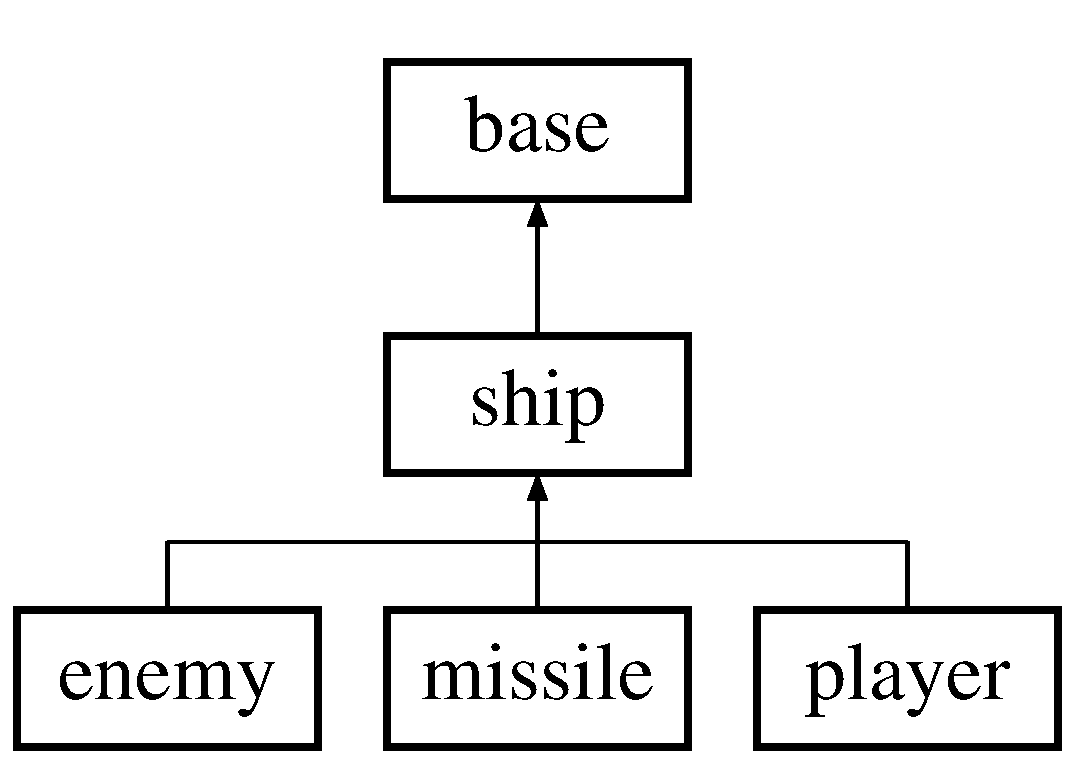
\includegraphics[height=3.000000cm]{classship}
\end{center}
\end{figure}
\subsection*{Public Member Functions}
\begin{DoxyCompactItemize}
\item 
\hyperlink{classship_a3ca9f0f5ecbed6a53d7bae37b8e57704}{ship} (const \hyperlink{structvec3}{vec3} \-\_\-p, const \hyperlink{ship_8hpp_af74a63841701826d661cb9809aaf7092}{ship\-\_\-spec} \-\_\-type, const float \-\_\-radius)
\begin{DoxyCompactList}\small\item\em ctor for the ship class. \end{DoxyCompactList}\item 
\hyperlink{classship_a2d79339fb680dce8b7b581103706c357}{ship} (const \hyperlink{classship}{ship} \&\-\_\-src, const \hyperlink{structvec3}{vec3} \-\_\-p)
\begin{DoxyCompactList}\small\item\em Copy ctor for the ship class. \end{DoxyCompactList}\item 
void \hyperlink{classship_a9c6d721f86324e034dd0c97deb903257}{add\-Vel\-S} (const \hyperlink{structvec3}{vec3} \-\_\-v)
\begin{DoxyCompactList}\small\item\em Adds velocity to the ship. \end{DoxyCompactList}\item 
void \hyperlink{classship_ac6075d376a2f10087a7daddd6dc4104e}{accelerate} (const float \-\_\-mult)
\begin{DoxyCompactList}\small\item\em Accelerates the ship, in the direction that it is facing. \end{DoxyCompactList}\item 
void \hyperlink{classship_a8ea8250d5797b7b3822997eca7059b6d}{accelerate} (const \hyperlink{structvec3}{vec3} \-\_\-dir, const float \-\_\-mult)
\begin{DoxyCompactList}\small\item\em Adds velocity to the ship. \end{DoxyCompactList}\item 
void \hyperlink{classship_a940069471464086ac4a47089c4ee7c1f}{set\-Accelerating} (const bool \-\_\-b)
\begin{DoxyCompactList}\small\item\em Setter for m\-\_\-accelerating. \end{DoxyCompactList}\item 
void \hyperlink{classship_a2e0ef103ac673f4cce05a364a1d5332e}{dodge} (const float \-\_\-side)
\begin{DoxyCompactList}\small\item\em Adds velocity to the ship, perpendicular to the direction in which it is facing. \end{DoxyCompactList}\item 
void \hyperlink{classship_a17c6d50f754a9d6466d315e74c8245dc}{update} (const float \-\_\-dt)
\begin{DoxyCompactList}\small\item\em Updates the ship. \end{DoxyCompactList}\item 
\hypertarget{classship_a85bbae8598da6aff13de499977174390}{void \hyperlink{classship_a85bbae8598da6aff13de499977174390}{set\-T\-Ang} (const float \-\_\-ang)}\label{classship_a85bbae8598da6aff13de499977174390}

\begin{DoxyCompactList}\small\item\em Getter and setter for m\-\_\-target\-Angle. \end{DoxyCompactList}\item 
\hypertarget{classship_abc03617c92eb7c1a3c818749681fec5c}{float {\bfseries get\-T\-Ang} () const }\label{classship_abc03617c92eb7c1a3c818749681fec5c}

\item 
\hypertarget{classship_a0b5042369840df23927f796b83ccde29}{void \hyperlink{classship_a0b5042369840df23927f796b83ccde29}{set\-Ang} (const float \-\_\-ang)}\label{classship_a0b5042369840df23927f796b83ccde29}

\begin{DoxyCompactList}\small\item\em Getter and setter for m\-\_\-angle. \end{DoxyCompactList}\item 
\hypertarget{classship_a43ce3e315c632d9fc13ea0b18b70b159}{float {\bfseries get\-Ang} () const }\label{classship_a43ce3e315c632d9fc13ea0b18b70b159}

\item 
void \hyperlink{classship_af16bf57c238b48028a8ca6a5d5aad5c1}{set\-Weap\-Data} (const int \-\_\-val, const int \-\_\-src)
\begin{DoxyCompactList}\small\item\em Sets weapon data for a weapon slot. \end{DoxyCompactList}\item 
\hypertarget{classship_a0b07c591c7fe869ef35b9d21dc774ead}{void \hyperlink{classship_a0b07c591c7fe869ef35b9d21dc774ead}{set\-Weap} (const int \-\_\-val)}\label{classship_a0b07c591c7fe869ef35b9d21dc774ead}

\begin{DoxyCompactList}\small\item\em Sets, increments the current weapon. \end{DoxyCompactList}\item 
\hypertarget{classship_a8cac59509b65e0aadcb30bd7206b6bbd}{void {\bfseries incr\-Weap} (const int \-\_\-val)}\label{classship_a8cac59509b65e0aadcb30bd7206b6bbd}

\item 
float \hyperlink{classship_a3376905d6b8e5428e9afb4c89d4b8ebb}{get\-Cur\-Weap\-Stat} (\hyperlink{weapons_8hpp_ac6523c0263d02b0fbdbe8b8e958a50b5}{W\-E\-A\-P\-O\-N\-\_\-\-S\-T\-A\-T} \-\_\-stat) const 
\begin{DoxyCompactList}\small\item\em Gets a stat from the active weapon. \end{DoxyCompactList}\item 
\hypertarget{classship_af49c18fa918ff3597b6adeef15c0483c}{std\-::array$<$ float, 4 $>$ \hyperlink{classship_af49c18fa918ff3597b6adeef15c0483c}{get\-Cur\-Weap\-Col} () const }\label{classship_af49c18fa918ff3597b6adeef15c0483c}

\begin{DoxyCompactList}\small\item\em Returns the colour of the current weapon. \end{DoxyCompactList}\item 
\hypertarget{classship_af33e5cfaec7c0ac036ecd1ca52d654a8}{std\-::array$<$ float, 4 $>$ \hyperlink{classship_af33e5cfaec7c0ac036ecd1ca52d654a8}{get\-Shield\-Col} () const }\label{classship_af33e5cfaec7c0ac036ecd1ca52d654a8}

\begin{DoxyCompactList}\small\item\em Returns the colour of the shield. \end{DoxyCompactList}\item 
\hypertarget{classship_aa8603eb9b3e23120b61c76379510a23f}{std\-::vector$<$ std\-::array$<$ float, 10 $>$ $>$ \hyperlink{classship_aa8603eb9b3e23120b61c76379510a23f}{get\-Weaps} () const }\label{classship_aa8603eb9b3e23120b61c76379510a23f}

\begin{DoxyCompactList}\small\item\em Returns array of all of the ships weapons. \end{DoxyCompactList}\item 
\hypertarget{classship_a30fc891ce056dab197aa2738a7c100aa}{std\-::array$<$ float, 10 $>$ \hyperlink{classship_a30fc891ce056dab197aa2738a7c100aa}{get\-Weap} () const }\label{classship_a30fc891ce056dab197aa2738a7c100aa}

\begin{DoxyCompactList}\small\item\em Returns all data concerning a specific weapon. \end{DoxyCompactList}\item 
\hypertarget{classship_ab6eddbf0796ca30adc6ac81927abc750}{int \hyperlink{classship_ab6eddbf0796ca30adc6ac81927abc750}{get\-Cur\-Weap} () const }\label{classship_ab6eddbf0796ca30adc6ac81927abc750}

\begin{DoxyCompactList}\small\item\em Returns current weapon index. \end{DoxyCompactList}\item 
\hypertarget{classship_aeb88d49d9a8cfb5d7f36665f1ff18858}{void \hyperlink{classship_aeb88d49d9a8cfb5d7f36665f1ff18858}{shoot} ()}\label{classship_aeb88d49d9a8cfb5d7f36665f1ff18858}

\begin{DoxyCompactList}\small\item\em Sets m\-\_\-draw\-Shot to 255. \end{DoxyCompactList}\item 
\hypertarget{classship_ad9ca88b4655b003dafb719cec3481efb}{void \hyperlink{classship_ad9ca88b4655b003dafb719cec3481efb}{set\-Firing} (const bool \-\_\-v)}\label{classship_ad9ca88b4655b003dafb719cec3481efb}

\begin{DoxyCompactList}\small\item\em Getter and setter for m\-\_\-shooting. \end{DoxyCompactList}\item 
\hypertarget{classship_a694bdcef07e84d7f581f1c2cbf7d6a79}{bool {\bfseries is\-Firing} () const }\label{classship_a694bdcef07e84d7f581f1c2cbf7d6a79}

\item 
\hypertarget{classship_a6a8eef4a53c952a18de54e9083b35dbd}{void \hyperlink{classship_a6a8eef4a53c952a18de54e9083b35dbd}{set\-Max\-Health} (const float \-\_\-h, const bool \-\_\-match)}\label{classship_a6a8eef4a53c952a18de54e9083b35dbd}

\begin{DoxyCompactList}\small\item\em Getter and setter for m\-\_\-max\-Health. \end{DoxyCompactList}\item 
\hypertarget{classship_a995188d2c9128c440ac34b316e6bfdf5}{float {\bfseries get\-Max\-Health} () const }\label{classship_a995188d2c9128c440ac34b316e6bfdf5}

\item 
\hypertarget{classship_af0c7edd4a30c5e270f5b57e222c316a1}{void \hyperlink{classship_af0c7edd4a30c5e270f5b57e222c316a1}{set\-Max\-Shield} (const float \-\_\-s, const bool \-\_\-match)}\label{classship_af0c7edd4a30c5e270f5b57e222c316a1}

\begin{DoxyCompactList}\small\item\em Getter and setter for m\-\_\-max\-Shield. \end{DoxyCompactList}\item 
\hypertarget{classship_ad469c878cc8090c424c89cbf3a96a063}{float {\bfseries get\-Max\-Shield} () const }\label{classship_ad469c878cc8090c424c89cbf3a96a063}

\item 
\hypertarget{classship_a634e621176733941096c05dfcf3bff83}{void \hyperlink{classship_a634e621176733941096c05dfcf3bff83}{set\-Max\-Energy} (const float \-\_\-e, const bool \-\_\-match)}\label{classship_a634e621176733941096c05dfcf3bff83}

\begin{DoxyCompactList}\small\item\em Getter and setter for m\-\_\-max\-Energy. \end{DoxyCompactList}\item 
\hypertarget{classship_a954fe1bf94be13826196c169250bd964}{float {\bfseries get\-Max\-Energy} () const }\label{classship_a954fe1bf94be13826196c169250bd964}

\item 
\hypertarget{classship_a211c3f3057bfa0edba1b308395fae839}{void \hyperlink{classship_a211c3f3057bfa0edba1b308395fae839}{set\-Health} (const float \-\_\-h)}\label{classship_a211c3f3057bfa0edba1b308395fae839}

\begin{DoxyCompactList}\small\item\em Getters and setters for m\-\_\-health. \end{DoxyCompactList}\item 
\hypertarget{classship_a62f52e8063ad01583c7b9fc3e5c2aca3}{float {\bfseries get\-Health} () const }\label{classship_a62f52e8063ad01583c7b9fc3e5c2aca3}

\item 
\hypertarget{classship_a879475726ca8825f5256d9bf77383da4}{void {\bfseries incr\-Health} (const float \-\_\-v)}\label{classship_a879475726ca8825f5256d9bf77383da4}

\item 
\hypertarget{classship_a96e9f6e8fae43c1fa8a03d490491b96c}{void \hyperlink{classship_a96e9f6e8fae43c1fa8a03d490491b96c}{set\-Shield} (const float \-\_\-s)}\label{classship_a96e9f6e8fae43c1fa8a03d490491b96c}

\begin{DoxyCompactList}\small\item\em Getter and setter for m\-\_\-health. \end{DoxyCompactList}\item 
\hypertarget{classship_a090f2e29fbd4c9467ce85cb7d328a0b8}{float {\bfseries get\-Shield} () const }\label{classship_a090f2e29fbd4c9467ce85cb7d328a0b8}

\item 
\hypertarget{classship_a8eba58ae69aa02a01cf1d01a143b7a78}{void \hyperlink{classship_a8eba58ae69aa02a01cf1d01a143b7a78}{set\-Energy} (const float \-\_\-e)}\label{classship_a8eba58ae69aa02a01cf1d01a143b7a78}

\begin{DoxyCompactList}\small\item\em Getter and setter for m\-\_\-energy. \end{DoxyCompactList}\item 
\hypertarget{classship_a5657cf00d4e80b03027e149c61624f54}{float {\bfseries get\-Energy} () const }\label{classship_a5657cf00d4e80b03027e149c61624f54}

\item 
\hypertarget{classship_a9d4cba0939f03d27c9f85d2ee6ca6d5f}{float \hyperlink{classship_a9d4cba0939f03d27c9f85d2ee6ca6d5f}{get\-Cooldown} () const }\label{classship_a9d4cba0939f03d27c9f85d2ee6ca6d5f}

\begin{DoxyCompactList}\small\item\em Getter and setter for m\-\_\-cooldown. \end{DoxyCompactList}\item 
\hypertarget{classship_af6a10864d7d030e6a31ff1362cab790b}{void {\bfseries set\-Cooldown} (const float \-\_\-f)}\label{classship_af6a10864d7d030e6a31ff1362cab790b}

\item 
\hypertarget{classship_a6a4075497f5bede29ad9e9e5cb339238}{void \hyperlink{classship_a6a4075497f5bede29ad9e9e5cb339238}{set\-Missiles} (const int \-\_\-m)}\label{classship_a6a4075497f5bede29ad9e9e5cb339238}

\begin{DoxyCompactList}\small\item\em Getters and setters for m\-\_\-missiles. \end{DoxyCompactList}\item 
\hypertarget{classship_af4263788f57fca762ce8e5b2972bcaa5}{void {\bfseries incr\-Missiles} (const int \-\_\-m)}\label{classship_af4263788f57fca762ce8e5b2972bcaa5}

\item 
\hypertarget{classship_ac2a1cdc999b5c9d1528d39485aa980de}{int {\bfseries get\-Missiles} () const }\label{classship_ac2a1cdc999b5c9d1528d39485aa980de}

\item 
\hypertarget{classship_ac48ed042184a82f48389d0d7f9d3cbef}{void \hyperlink{classship_ac48ed042184a82f48389d0d7f9d3cbef}{set\-Energy\-Priority} (const int \-\_\-v)}\label{classship_ac48ed042184a82f48389d0d7f9d3cbef}

\begin{DoxyCompactList}\small\item\em Getter and setter for m\-\_\-priority. \end{DoxyCompactList}\item 
\hypertarget{classship_a7350a3e1ccf4042f84b3c1c9630835a4}{int {\bfseries get\-Energy\-Priority} () const }\label{classship_a7350a3e1ccf4042f84b3c1c9630835a4}

\item 
void \hyperlink{classship_aa6750a5206440d777ac933e282f6479f}{damage} (const float \-\_\-d)
\begin{DoxyCompactList}\small\item\em Damages the ship. \end{DoxyCompactList}\item 
void \hyperlink{classship_ae365ae5221a1bee3b46f76e00e3aba31}{damage} (const float \-\_\-d, const \hyperlink{structvec2}{vec2} \-\_\-v)
\begin{DoxyCompactList}\small\item\em Damages the ship. \end{DoxyCompactList}\item 
\hypertarget{classship_a487b3030a123fb11d5173b039621cf30}{int \hyperlink{classship_a487b3030a123fb11d5173b039621cf30}{get\-Upgrade} (const int \-\_\-index)}\label{classship_a487b3030a123fb11d5173b039621cf30}

\begin{DoxyCompactList}\small\item\em Getters and setters for m\-\_\-upgrades. \end{DoxyCompactList}\item 
\hypertarget{classship_a2f0eebc8a3a9908bfbdea941a24798fa}{void {\bfseries set\-Grade\-Arr} (const int \-\_\-i, const int \-\_\-v)}\label{classship_a2f0eebc8a3a9908bfbdea941a24798fa}

\item 
\hypertarget{classship_a9304f314a13a2a81f73472d9530d0efb}{void {\bfseries set\-Grade} (const int \-\_\-i, const int \-\_\-v)}\label{classship_a9304f314a13a2a81f73472d9530d0efb}

\item 
int \hyperlink{classship_a3f99b4cc97a783e997e280667a884d8f}{upgrade} (const int \-\_\-i)
\begin{DoxyCompactList}\small\item\em Upgrades the ship. \end{DoxyCompactList}\item 
\hypertarget{classship_aacfbddf2d0b29db49f62523e9d60af9c}{void \hyperlink{classship_aacfbddf2d0b29db49f62523e9d60af9c}{set\-Inertia} (const float \-\_\-in)}\label{classship_aacfbddf2d0b29db49f62523e9d60af9c}

\begin{DoxyCompactList}\small\item\em Getter and setter for m\-\_\-inertia. \end{DoxyCompactList}\item 
\hypertarget{classship_ad65743d746abadc12bf2c24cf465bfcd}{float {\bfseries get\-Inertia} () const }\label{classship_ad65743d746abadc12bf2c24cf465bfcd}

\item 
\hypertarget{classship_af1a5baf45ce6abd307284d604fc03685}{void \hyperlink{classship_af1a5baf45ce6abd307284d604fc03685}{set\-Generator\-Mul} (float \-\_\-g)}\label{classship_af1a5baf45ce6abd307284d604fc03685}

\begin{DoxyCompactList}\small\item\em Setter for generator multiplier. \end{DoxyCompactList}\item 
\hypertarget{classship_a336b4c1483e8d38bb53e611e6e16e737}{void \hyperlink{classship_a336b4c1483e8d38bb53e611e6e16e737}{set\-Engine\-Power} (const float \-\_\-val)}\label{classship_a336b4c1483e8d38bb53e611e6e16e737}

\begin{DoxyCompactList}\small\item\em Getter and setter for m\-\_\-engine\-Power. \end{DoxyCompactList}\item 
\hypertarget{classship_a472e2517a1285ba9b61d476233aef9c2}{float {\bfseries get\-Engine\-Power} () const }\label{classship_a472e2517a1285ba9b61d476233aef9c2}

\item 
\hypertarget{classship_a68b49f5befb6f882b2900d47d0f8a960}{\hyperlink{ship_8hpp_af74a63841701826d661cb9809aaf7092}{ship\-\_\-spec} \hyperlink{classship_a68b49f5befb6f882b2900d47d0f8a960}{get\-Classification} () const }\label{classship_a68b49f5befb6f882b2900d47d0f8a960}

\begin{DoxyCompactList}\small\item\em m\-\_\-classification getter. \end{DoxyCompactList}\item 
\hypertarget{classship_ab247165c9c55d122195cd4edec0d823d}{float \hyperlink{classship_ab247165c9c55d122195cd4edec0d823d}{get\-Radius} () const }\label{classship_ab247165c9c55d122195cd4edec0d823d}

\begin{DoxyCompactList}\small\item\em m\-\_\-radius getter. \end{DoxyCompactList}\item 
\hypertarget{classship_a905701667792667dd63e676e97864c15}{int \hyperlink{classship_a905701667792667dd63e676e97864c15}{get\-Score} () const }\label{classship_a905701667792667dd63e676e97864c15}

\begin{DoxyCompactList}\small\item\em Returns the score value for the ship, how many points the player gets for blowing it up. \end{DoxyCompactList}\item 
\hypertarget{classship_ab752c545e9f8a22fecff63dc77c3a5a9}{float \hyperlink{classship_ab752c545e9f8a22fecff63dc77c3a5a9}{get\-Ang\-Vel} () const }\label{classship_ab752c545e9f8a22fecff63dc77c3a5a9}

\begin{DoxyCompactList}\small\item\em Getter for m\-\_\-ang\-Vel. \end{DoxyCompactList}\item 
\hypertarget{classship_ae4232335b58866673ca45bb42e35c2a2}{bool \hyperlink{classship_ae4232335b58866673ca45bb42e35c2a2}{get\-Can\-Move} () const }\label{classship_ae4232335b58866673ca45bb42e35c2a2}

\begin{DoxyCompactList}\small\item\em Getter for m\-\_\-can\-Move. \end{DoxyCompactList}\item 
\hypertarget{classship_abe8c5d20cef002bb0013a33253cff7c4}{bool \hyperlink{classship_abe8c5d20cef002bb0013a33253cff7c4}{get\-Can\-Shoot} () const }\label{classship_abe8c5d20cef002bb0013a33253cff7c4}

\begin{DoxyCompactList}\small\item\em Getter for m\-\_\-can\-Shoot. \end{DoxyCompactList}\item 
\hypertarget{classship_ad86c5ef782779451e8539c44b9a23123}{bool \hyperlink{classship_ad86c5ef782779451e8539c44b9a23123}{in\-Combat} ()}\label{classship_ad86c5ef782779451e8539c44b9a23123}

\begin{DoxyCompactList}\small\item\em Whether the ship can be considered to be in combat. \end{DoxyCompactList}\item 
\hypertarget{classship_ab954d0adc48f4b6a358863969a40d478}{std\-::string \hyperlink{classship_ab954d0adc48f4b6a358863969a40d478}{get\-Identifier} () const }\label{classship_ab954d0adc48f4b6a358863969a40d478}

\begin{DoxyCompactList}\small\item\em Getter for the ship type id. \end{DoxyCompactList}\item 
\hypertarget{classship_a92cdedc492085eab5448222e5dc36296}{std\-::array$<$ float, 4 $>$ \hyperlink{classship_a92cdedc492085eab5448222e5dc36296}{get\-Alpha\-Stats} () const }\label{classship_a92cdedc492085eab5448222e5dc36296}

\begin{DoxyCompactList}\small\item\em Gets the alpha values for various colours associated with the ship. \end{DoxyCompactList}\item 
\hypertarget{classship_a1e4b3788fa205b41bad280859827d802}{float \hyperlink{classship_a1e4b3788fa205b41bad280859827d802}{get\-Shield\-Glow} () const }\label{classship_a1e4b3788fa205b41bad280859827d802}

\begin{DoxyCompactList}\small\item\em Getter for m\-\_\-shield\-Glow. \end{DoxyCompactList}\item 
\hypertarget{classship_a2a92ab0c77d62a5132ac69c19cb51292}{float \hyperlink{classship_a2a92ab0c77d62a5132ac69c19cb51292}{get\-Laser\-Glow} () const }\label{classship_a2a92ab0c77d62a5132ac69c19cb51292}

\begin{DoxyCompactList}\small\item\em Getter for m\-\_\-draw\-Shot, converts it to the range 0-\/1. \end{DoxyCompactList}\item 
\hypertarget{classship_ae9df18aea813f1007ab94462dec47c57}{bool \hyperlink{classship_ae9df18aea813f1007ab94462dec47c57}{has\-Parent} () const }\label{classship_ae9df18aea813f1007ab94462dec47c57}

\begin{DoxyCompactList}\small\item\em Getters and setters for parents. \end{DoxyCompactList}\item 
\hypertarget{classship_a5a8a7ba1a0fc40f976c1e00e6483efde}{long int {\bfseries get\-Parent} () const }\label{classship_a5a8a7ba1a0fc40f976c1e00e6483efde}

\item 
\hypertarget{classship_a4ce26110be178f9d91b0b063703fbf41}{void {\bfseries set\-Parent} (long int \-\_\-p)}\label{classship_a4ce26110be178f9d91b0b063703fbf41}

\item 
\hypertarget{classship_a26410a4b84949c59af4c942b39a91986}{\hyperlink{structvec3}{vec3} \hyperlink{classship_a26410a4b84949c59af4c942b39a91986}{get\-Parent\-Offset} ()}\label{classship_a26410a4b84949c59af4c942b39a91986}

\begin{DoxyCompactList}\small\item\em Getters and setters for parent offsets. \end{DoxyCompactList}\item 
\hypertarget{classship_abf758a42fb1802a44657a5174800640d}{void {\bfseries set\-Parent\-Offset} (\hyperlink{structvec3}{vec3} \-\_\-v)}\label{classship_abf758a42fb1802a44657a5174800640d}

\item 
\hypertarget{classship_a1b119471128280ae9527949e95fbaca3}{long unsigned int \hyperlink{classship_a1b119471128280ae9527949e95fbaca3}{get\-Unique\-I\-D} ()}\label{classship_a1b119471128280ae9527949e95fbaca3}

\begin{DoxyCompactList}\small\item\em Getter for unique I\-D. \end{DoxyCompactList}\end{DoxyCompactItemize}


\subsection{Detailed Description}
Inherits from ship, contains data such as weapon type, engine power, shield strength. It does not, however, contain any functionality to behave autonomously. 

\subsection{Constructor \& Destructor Documentation}
\hypertarget{classship_a3ca9f0f5ecbed6a53d7bae37b8e57704}{\index{ship@{ship}!ship@{ship}}
\index{ship@{ship}!ship@{ship}}
\subsubsection[{ship}]{\setlength{\rightskip}{0pt plus 5cm}ship\-::ship (
\begin{DoxyParamCaption}
\item[{const {\bf vec3}}]{\-\_\-p, }
\item[{const {\bf ship\-\_\-spec}}]{\-\_\-type, }
\item[{const float}]{\-\_\-radius}
\end{DoxyParamCaption}
)}}\label{classship_a3ca9f0f5ecbed6a53d7bae37b8e57704}


ctor for the ship class. 


\begin{DoxyParams}{Parameters}
{\em \-\_\-p} & position \\
\hline
{\em \-\_\-type} & ship type \\
\hline
{\em \-\_\-radius} & ship size \\
\hline
\end{DoxyParams}
\hypertarget{classship_a2d79339fb680dce8b7b581103706c357}{\index{ship@{ship}!ship@{ship}}
\index{ship@{ship}!ship@{ship}}
\subsubsection[{ship}]{\setlength{\rightskip}{0pt plus 5cm}ship\-::ship (
\begin{DoxyParamCaption}
\item[{const {\bf ship} \&}]{\-\_\-src, }
\item[{const {\bf vec3}}]{\-\_\-p}
\end{DoxyParamCaption}
)}}\label{classship_a2d79339fb680dce8b7b581103706c357}


Copy ctor for the ship class. 


\begin{DoxyParams}{Parameters}
{\em \-\_\-src} & source object \\
\hline
{\em \-\_\-p} & position \\
\hline
\end{DoxyParams}


\subsection{Member Function Documentation}
\hypertarget{classship_ac6075d376a2f10087a7daddd6dc4104e}{\index{ship@{ship}!accelerate@{accelerate}}
\index{accelerate@{accelerate}!ship@{ship}}
\subsubsection[{accelerate}]{\setlength{\rightskip}{0pt plus 5cm}void ship\-::accelerate (
\begin{DoxyParamCaption}
\item[{const float}]{\-\_\-mult}
\end{DoxyParamCaption}
)}}\label{classship_ac6075d376a2f10087a7daddd6dc4104e}


Accelerates the ship, in the direction that it is facing. 


\begin{DoxyParams}{Parameters}
{\em \-\_\-mult} & multiplier \\
\hline
\end{DoxyParams}
\hypertarget{classship_a8ea8250d5797b7b3822997eca7059b6d}{\index{ship@{ship}!accelerate@{accelerate}}
\index{accelerate@{accelerate}!ship@{ship}}
\subsubsection[{accelerate}]{\setlength{\rightskip}{0pt plus 5cm}void ship\-::accelerate (
\begin{DoxyParamCaption}
\item[{const {\bf vec3}}]{\-\_\-dir, }
\item[{const float}]{\-\_\-mult}
\end{DoxyParamCaption}
)}}\label{classship_a8ea8250d5797b7b3822997eca7059b6d}


Adds velocity to the ship. 


\begin{DoxyParams}{Parameters}
{\em \-\_\-dir} & base vector \\
\hline
{\em \-\_\-mult} & multiplier \\
\hline
\end{DoxyParams}
\hypertarget{classship_a9c6d721f86324e034dd0c97deb903257}{\index{ship@{ship}!add\-Vel\-S@{add\-Vel\-S}}
\index{add\-Vel\-S@{add\-Vel\-S}!ship@{ship}}
\subsubsection[{add\-Vel\-S}]{\setlength{\rightskip}{0pt plus 5cm}void ship\-::add\-Vel\-S (
\begin{DoxyParamCaption}
\item[{const {\bf vec3}}]{\-\_\-v}
\end{DoxyParamCaption}
)\hspace{0.3cm}{\ttfamily [inline]}}}\label{classship_a9c6d721f86324e034dd0c97deb903257}


Adds velocity to the ship. 


\begin{DoxyParams}{Parameters}
{\em \-\_\-v} & base vector \\
\hline
\end{DoxyParams}
\hypertarget{classship_aa6750a5206440d777ac933e282f6479f}{\index{ship@{ship}!damage@{damage}}
\index{damage@{damage}!ship@{ship}}
\subsubsection[{damage}]{\setlength{\rightskip}{0pt plus 5cm}void ship\-::damage (
\begin{DoxyParamCaption}
\item[{const float}]{\-\_\-d}
\end{DoxyParamCaption}
)}}\label{classship_aa6750a5206440d777ac933e282f6479f}


Damages the ship. 


\begin{DoxyParams}{Parameters}
{\em \-\_\-d} & damage \\
\hline
\end{DoxyParams}
\hypertarget{classship_ae365ae5221a1bee3b46f76e00e3aba31}{\index{ship@{ship}!damage@{damage}}
\index{damage@{damage}!ship@{ship}}
\subsubsection[{damage}]{\setlength{\rightskip}{0pt plus 5cm}void ship\-::damage (
\begin{DoxyParamCaption}
\item[{const float}]{\-\_\-d, }
\item[{const {\bf vec2}}]{\-\_\-v}
\end{DoxyParamCaption}
)}}\label{classship_ae365ae5221a1bee3b46f76e00e3aba31}


Damages the ship. 


\begin{DoxyParams}{Parameters}
{\em \-\_\-d} & damage, \-\_\-v knockback vector \\
\hline
\end{DoxyParams}
\hypertarget{classship_a2e0ef103ac673f4cce05a364a1d5332e}{\index{ship@{ship}!dodge@{dodge}}
\index{dodge@{dodge}!ship@{ship}}
\subsubsection[{dodge}]{\setlength{\rightskip}{0pt plus 5cm}void ship\-::dodge (
\begin{DoxyParamCaption}
\item[{const float}]{\-\_\-side}
\end{DoxyParamCaption}
)}}\label{classship_a2e0ef103ac673f4cce05a364a1d5332e}


Adds velocity to the ship, perpendicular to the direction in which it is facing. 


\begin{DoxyParams}{Parameters}
{\em \-\_\-side} & multiplier \\
\hline
\end{DoxyParams}
\hypertarget{classship_a3376905d6b8e5428e9afb4c89d4b8ebb}{\index{ship@{ship}!get\-Cur\-Weap\-Stat@{get\-Cur\-Weap\-Stat}}
\index{get\-Cur\-Weap\-Stat@{get\-Cur\-Weap\-Stat}!ship@{ship}}
\subsubsection[{get\-Cur\-Weap\-Stat}]{\setlength{\rightskip}{0pt plus 5cm}float ship\-::get\-Cur\-Weap\-Stat (
\begin{DoxyParamCaption}
\item[{{\bf W\-E\-A\-P\-O\-N\-\_\-\-S\-T\-A\-T}}]{\-\_\-stat}
\end{DoxyParamCaption}
) const}}\label{classship_a3376905d6b8e5428e9afb4c89d4b8ebb}


Gets a stat from the active weapon. 


\begin{DoxyParams}{Parameters}
{\em \-\_\-stat} & weapon stat to retrieve (enum defined in \hyperlink{weapons_8hpp}{weapons.\-hpp}) \\
\hline
\end{DoxyParams}
\hypertarget{classship_a940069471464086ac4a47089c4ee7c1f}{\index{ship@{ship}!set\-Accelerating@{set\-Accelerating}}
\index{set\-Accelerating@{set\-Accelerating}!ship@{ship}}
\subsubsection[{set\-Accelerating}]{\setlength{\rightskip}{0pt plus 5cm}void ship\-::set\-Accelerating (
\begin{DoxyParamCaption}
\item[{const bool}]{\-\_\-b}
\end{DoxyParamCaption}
)\hspace{0.3cm}{\ttfamily [inline]}}}\label{classship_a940069471464086ac4a47089c4ee7c1f}


Setter for m\-\_\-accelerating. 


\begin{DoxyParams}{Parameters}
{\em \-\_\-b} & input \\
\hline
\end{DoxyParams}
\hypertarget{classship_af16bf57c238b48028a8ca6a5d5aad5c1}{\index{ship@{ship}!set\-Weap\-Data@{set\-Weap\-Data}}
\index{set\-Weap\-Data@{set\-Weap\-Data}!ship@{ship}}
\subsubsection[{set\-Weap\-Data}]{\setlength{\rightskip}{0pt plus 5cm}void ship\-::set\-Weap\-Data (
\begin{DoxyParamCaption}
\item[{const int}]{\-\_\-val, }
\item[{const int}]{\-\_\-src}
\end{DoxyParamCaption}
)\hspace{0.3cm}{\ttfamily [inline]}}}\label{classship_af16bf57c238b48028a8ca6a5d5aad5c1}


Sets weapon data for a weapon slot. 


\begin{DoxyParams}{Parameters}
{\em \-\_\-val} & weapon slot to fill \\
\hline
{\em \-\_\-src} & source index from global weapon data array (\hyperlink{weapons_8hpp}{weapons.\-hpp}) \\
\hline
\end{DoxyParams}
\hypertarget{classship_a17c6d50f754a9d6466d315e74c8245dc}{\index{ship@{ship}!update@{update}}
\index{update@{update}!ship@{ship}}
\subsubsection[{update}]{\setlength{\rightskip}{0pt plus 5cm}void ship\-::update (
\begin{DoxyParamCaption}
\item[{const float}]{\-\_\-dt}
\end{DoxyParamCaption}
)}}\label{classship_a17c6d50f754a9d6466d315e74c8245dc}


Updates the ship. 


\begin{DoxyParams}{Parameters}
{\em \-\_\-dt} & time-\/step \\
\hline
\end{DoxyParams}
\hypertarget{classship_a3f99b4cc97a783e997e280667a884d8f}{\index{ship@{ship}!upgrade@{upgrade}}
\index{upgrade@{upgrade}!ship@{ship}}
\subsubsection[{upgrade}]{\setlength{\rightskip}{0pt plus 5cm}int ship\-::upgrade (
\begin{DoxyParamCaption}
\item[{const int}]{\-\_\-i}
\end{DoxyParamCaption}
)}}\label{classship_a3f99b4cc97a783e997e280667a884d8f}


Upgrades the ship. 


\begin{DoxyParams}{Parameters}
{\em \-\_\-i} & slot to upgrade \\
\hline
\end{DoxyParams}


The documentation for this class was generated from the following files\-:\begin{DoxyCompactItemize}
\item 
include/\hyperlink{ship_8hpp}{ship.\-hpp}\item 
src/ship.\-cpp\end{DoxyCompactItemize}

\hypertarget{classsim__time}{\section{sim\-\_\-time Class Reference}
\label{classsim__time}\index{sim\-\_\-time@{sim\-\_\-time}}
}


Used to control time-\/stepping in-\/game. Also stores some values it probably needn't, since they aren't strictly necessary for the class to function, but I found it useful to have them all in one place.  




{\ttfamily \#include $<$sim\-\_\-time.\-hpp$>$}

\subsection*{Public Member Functions}
\begin{DoxyCompactItemize}
\item 
\hyperlink{classsim__time_a42885957f994feacfe3ae4246875be6a}{sim\-\_\-time} (float \-\_\-fps)
\begin{DoxyCompactList}\small\item\em ctor for the \hyperlink{classsim__time}{sim\-\_\-time} class. \end{DoxyCompactList}\item 
\hypertarget{classsim__time_ae4e4e0ec9b08c69ed694fc55af087d8f}{void \hyperlink{classsim__time_ae4e4e0ec9b08c69ed694fc55af087d8f}{set\-Start} ()}\label{classsim__time_ae4e4e0ec9b08c69ed694fc55af087d8f}

\begin{DoxyCompactList}\small\item\em Setter for m\-\_\-start, also recalculates m\-\_\-diff and m\-\_\-time\-\_\-since\-\_\-creation. \end{DoxyCompactList}\item 
\hypertarget{classsim__time_a53ec26919841cbb2eb4aeca2b4839e95}{void \hyperlink{classsim__time_a53ec26919841cbb2eb4aeca2b4839e95}{set\-Cur} ()}\label{classsim__time_a53ec26919841cbb2eb4aeca2b4839e95}

\begin{DoxyCompactList}\small\item\em Setter for m\-\_\-cur, also recalculates m\-\_\-diff and m\-\_\-time\-\_\-since\-\_\-creation. \end{DoxyCompactList}\item 
\hypertarget{classsim__time_a3dfeae677bf25cc05120a70d03c0e1f2}{double \hyperlink{classsim__time_a3dfeae677bf25cc05120a70d03c0e1f2}{get\-Diff} () const }\label{classsim__time_a3dfeae677bf25cc05120a70d03c0e1f2}

\begin{DoxyCompactList}\small\item\em Getter for m\-\_\-diff. \end{DoxyCompactList}\item 
\hypertarget{classsim__time_af2a38a2f13c8f49d2b2f1185e5e6f185}{double \hyperlink{classsim__time_af2a38a2f13c8f49d2b2f1185e5e6f185}{get\-Time} () const }\label{classsim__time_af2a38a2f13c8f49d2b2f1185e5e6f185}

\begin{DoxyCompactList}\small\item\em Getter for m\-\_\-time\-\_\-since\-\_\-creation. \end{DoxyCompactList}\item 
\hypertarget{classsim__time_a98cee05c12e80d66458df3d1ac98b0b7}{double \hyperlink{classsim__time_a98cee05c12e80d66458df3d1ac98b0b7}{get\-Frame} () const }\label{classsim__time_a98cee05c12e80d66458df3d1ac98b0b7}

\begin{DoxyCompactList}\small\item\em Getter for m\-\_\-sim\-\_\-dt. \end{DoxyCompactList}\item 
\hypertarget{classsim__time_a1b2c3fecdfbd433fb66c314ed8906e1b}{double \hyperlink{classsim__time_a1b2c3fecdfbd433fb66c314ed8906e1b}{get\-Acc} () const }\label{classsim__time_a1b2c3fecdfbd433fb66c314ed8906e1b}

\begin{DoxyCompactList}\small\item\em Getter for m\-\_\-sim\-\_\-accumulator. \end{DoxyCompactList}\item 
void \hyperlink{classsim__time_a5044d04f14dd03986a67340eef498a24}{incr\-Acc} (float \-\_\-incr)
\begin{DoxyCompactList}\small\item\em Increments m\-\_\-sim\-\_\-accumulator by a given value. \end{DoxyCompactList}\end{DoxyCompactItemize}


\subsection{Detailed Description}
Used to control time-\/stepping in-\/game. Also stores some values it probably needn't, since they aren't strictly necessary for the class to function, but I found it useful to have them all in one place. 

\subsection{Constructor \& Destructor Documentation}
\hypertarget{classsim__time_a42885957f994feacfe3ae4246875be6a}{\index{sim\-\_\-time@{sim\-\_\-time}!sim\-\_\-time@{sim\-\_\-time}}
\index{sim\-\_\-time@{sim\-\_\-time}!sim_time@{sim\-\_\-time}}
\subsubsection[{sim\-\_\-time}]{\setlength{\rightskip}{0pt plus 5cm}sim\-\_\-time\-::sim\-\_\-time (
\begin{DoxyParamCaption}
\item[{float}]{\-\_\-fps}
\end{DoxyParamCaption}
)}}\label{classsim__time_a42885957f994feacfe3ae4246875be6a}


ctor for the \hyperlink{classsim__time}{sim\-\_\-time} class. 


\begin{DoxyParams}{Parameters}
{\em \-\_\-fps} & Stores the fps at which we will update the game. \\
\hline
\end{DoxyParams}


\subsection{Member Function Documentation}
\hypertarget{classsim__time_a5044d04f14dd03986a67340eef498a24}{\index{sim\-\_\-time@{sim\-\_\-time}!incr\-Acc@{incr\-Acc}}
\index{incr\-Acc@{incr\-Acc}!sim_time@{sim\-\_\-time}}
\subsubsection[{incr\-Acc}]{\setlength{\rightskip}{0pt plus 5cm}void sim\-\_\-time\-::incr\-Acc (
\begin{DoxyParamCaption}
\item[{float}]{\-\_\-incr}
\end{DoxyParamCaption}
)\hspace{0.3cm}{\ttfamily [inline]}}}\label{classsim__time_a5044d04f14dd03986a67340eef498a24}


Increments m\-\_\-sim\-\_\-accumulator by a given value. 


\begin{DoxyParams}{Parameters}
{\em \-\_\-incr} & Increment value \\
\hline
\end{DoxyParams}


The documentation for this class was generated from the following files\-:\begin{DoxyCompactItemize}
\item 
include/\hyperlink{sim__time_8hpp}{sim\-\_\-time.\-hpp}\item 
src/sim\-\_\-time.\-cpp\end{DoxyCompactItemize}

\hypertarget{structsprite__sheet}{\section{sprite\-\_\-sheet Class Reference}
\label{structsprite__sheet}\index{sprite\-\_\-sheet@{sprite\-\_\-sheet}}
}


Stores a bunch of S\-D\-L\-\_\-\-Textures, and the functionality to destroy them. The functionality to fill them is actually stores in the renderer class, although I suppose I could move it here. Used mainly to draw text.  




{\ttfamily \#include $<$sprite\-\_\-sheet.\-hpp$>$}

\subsection*{Public Member Functions}
\begin{DoxyCompactItemize}
\item 
\hypertarget{structsprite__sheet_af199744dfbd8b4efe3d5170f92e8bff3}{void \hyperlink{structsprite__sheet_af199744dfbd8b4efe3d5170f92e8bff3}{destroy} ()}\label{structsprite__sheet_af199744dfbd8b4efe3d5170f92e8bff3}

\begin{DoxyCompactList}\small\item\em Destroys the textures in m\-\_\-sheet. \end{DoxyCompactList}\end{DoxyCompactItemize}
\subsection*{Public Attributes}
\begin{DoxyCompactItemize}
\item 
\hypertarget{structsprite__sheet_a5979f53ad0519486d63e9473a62e08c2}{std\-::vector$<$ S\-D\-L\-\_\-\-Texture $\ast$ $>$ \hyperlink{structsprite__sheet_a5979f53ad0519486d63e9473a62e08c2}{m\-\_\-sheet}}\label{structsprite__sheet_a5979f53ad0519486d63e9473a62e08c2}

\begin{DoxyCompactList}\small\item\em Storage for the sdl textures. \end{DoxyCompactList}\end{DoxyCompactItemize}


\subsection{Detailed Description}
Stores a bunch of S\-D\-L\-\_\-\-Textures, and the functionality to destroy them. The functionality to fill them is actually stores in the renderer class, although I suppose I could move it here. Used mainly to draw text. 

The documentation for this class was generated from the following files\-:\begin{DoxyCompactItemize}
\item 
include/\hyperlink{sprite__sheet_8hpp}{sprite\-\_\-sheet.\-hpp}\item 
src/sprite\-\_\-sheet.\-cpp\end{DoxyCompactItemize}

\hypertarget{structsprite_sheet}{\section{sprite\-Sheet Class Reference}
\label{structsprite_sheet}\index{sprite\-Sheet@{sprite\-Sheet}}
}


Stores a bunch of opengl textures, and their dimensions. Used mainly to draw text.  




{\ttfamily \#include $<$sprite\-\_\-sheet\-\_\-opengl.\-hpp$>$}

\subsection*{Public Attributes}
\begin{DoxyCompactItemize}
\item 
\hypertarget{structsprite_sheet_a9888d63a720d99dc77dcdce9f5d423e6}{std\-::vector$<$ std\-::pair$<$ int, \\*
int $>$ $>$ \hyperlink{structsprite_sheet_a9888d63a720d99dc77dcdce9f5d423e6}{m\-\_\-dim}}\label{structsprite_sheet_a9888d63a720d99dc77dcdce9f5d423e6}

\begin{DoxyCompactList}\small\item\em \hyperlink{struct_container}{Container} of dimensions, matching indexes with texture vector. \end{DoxyCompactList}\item 
\hypertarget{structsprite_sheet_aae42c60737eae96af8c246e166504e91}{std\-::vector$<$ G\-Luint $>$ \hyperlink{structsprite_sheet_aae42c60737eae96af8c246e166504e91}{m\-\_\-sheet}}\label{structsprite_sheet_aae42c60737eae96af8c246e166504e91}

\begin{DoxyCompactList}\small\item\em Storage for opengl texture I\-Ds. \end{DoxyCompactList}\end{DoxyCompactItemize}


\subsection{Detailed Description}
Stores a bunch of opengl textures, and their dimensions. Used mainly to draw text. 

The documentation for this class was generated from the following file\-:\begin{DoxyCompactItemize}
\item 
include/sprite\-\_\-sheet\-\_\-opengl.\-hpp\end{DoxyCompactItemize}

\hypertarget{structsquad}{\section{squad Class Reference}
\label{structsquad}\index{squad@{squad}}
}


Contains data that allows enemies to coordinate with one another. Also has a unique I\-D, and ships in the squad are tagged with this.  




{\ttfamily \#include $<$squad.\-hpp$>$}

\subsection*{Public Attributes}
\begin{DoxyCompactItemize}
\item 
\hypertarget{structsquad_a7462a498cd5e759746adc25e312156c4}{int \hyperlink{structsquad_a7462a498cd5e759746adc25e312156c4}{m\-\_\-id}}\label{structsquad_a7462a498cd5e759746adc25e312156c4}

\begin{DoxyCompactList}\small\item\em The unique I\-D for the squad. Rather than have the squad actually contain its ships, I opted for a shallower structure to facilitate interaction between agents. \end{DoxyCompactList}\item 
\hypertarget{structsquad_a480945019f91f6cd4e71c9a632f4090a}{int \hyperlink{structsquad_a480945019f91f6cd4e71c9a632f4090a}{m\-\_\-size}}\label{structsquad_a480945019f91f6cd4e71c9a632f4090a}

\begin{DoxyCompactList}\small\item\em The number of ships in the squad. \end{DoxyCompactList}\item 
\hypertarget{structsquad_a470eb2e3b7123f5b565f36bf24e8c41d}{int \hyperlink{structsquad_a470eb2e3b7123f5b565f36bf24e8c41d}{m\-\_\-max\-\_\-size}}\label{structsquad_a470eb2e3b7123f5b565f36bf24e8c41d}

\begin{DoxyCompactList}\small\item\em The max size for the squad. \end{DoxyCompactList}\item 
\hypertarget{structsquad_a6c73412eccda20dac696566e6e6716a8}{\hyperlink{enemy_8hpp_abac1fdbabb5a6be5f0d6ae40be5c5a58}{ai\-Team} \hyperlink{structsquad_a6c73412eccda20dac696566e6e6716a8}{m\-\_\-team}}\label{structsquad_a6c73412eccda20dac696566e6e6716a8}

\begin{DoxyCompactList}\small\item\em The team that the squad is on. \end{DoxyCompactList}\item 
\hypertarget{structsquad_a99940fccf13785ab516fdf4afc68e328}{\hyperlink{enemy_8hpp_a6e73eb3e8e86f5922e45adeb450ceb1e}{ai\-Goal} \hyperlink{structsquad_a99940fccf13785ab516fdf4afc68e328}{m\-\_\-squad\-Goal}}\label{structsquad_a99940fccf13785ab516fdf4afc68e328}

\begin{DoxyCompactList}\small\item\em The currents goal, used to coordinate member behaviours. \end{DoxyCompactList}\item 
\hypertarget{structsquad_ae5836de9f2556e38d2e9b78fda8c3abd}{\hyperlink{structvec3}{vec3} \hyperlink{structsquad_ae5836de9f2556e38d2e9b78fda8c3abd}{m\-\_\-center\-Point}}\label{structsquad_ae5836de9f2556e38d2e9b78fda8c3abd}

\begin{DoxyCompactList}\small\item\em Typically set to the average position of the members, this acts as the squad center. Could conceivably be set to leader position to alter behaviour. \end{DoxyCompactList}\item 
\hypertarget{structsquad_ab0584c31fa3c89a99dc700d830619816}{\hyperlink{structvec3}{vec3} \hyperlink{structsquad_ab0584c31fa3c89a99dc700d830619816}{m\-\_\-average\-Vel}}\label{structsquad_ab0584c31fa3c89a99dc700d830619816}

\begin{DoxyCompactList}\small\item\em The average velocity of the members. Useful for Craig-\/\-Reynolds-\/eque alignment. \end{DoxyCompactList}\item 
\hypertarget{structsquad_a53048bfba949abf5351e18982ca34d22}{float \hyperlink{structsquad_a53048bfba949abf5351e18982ca34d22}{m\-\_\-regroup\-Dist} = 2000.\-0f}\label{structsquad_a53048bfba949abf5351e18982ca34d22}

\begin{DoxyCompactList}\small\item\em Ships further than this distance from the squad center will attempt to regroup. \end{DoxyCompactList}\item 
\hypertarget{structsquad_a7e29621628f833feb8fd24525e044586}{float \hyperlink{structsquad_a7e29621628f833feb8fd24525e044586}{m\-\_\-strength}}\label{structsquad_a7e29621628f833feb8fd24525e044586}

\begin{DoxyCompactList}\small\item\em Perceived strength of the squad, affects morale. \end{DoxyCompactList}\end{DoxyCompactItemize}


\subsection{Detailed Description}
Contains data that allows enemies to coordinate with one another. Also has a unique I\-D, and ships in the squad are tagged with this. 

The documentation for this class was generated from the following file\-:\begin{DoxyCompactItemize}
\item 
include/\hyperlink{squad_8hpp}{squad.\-hpp}\end{DoxyCompactItemize}

\hypertarget{classstardust}{\section{stardust Class Reference}
\label{classstardust}\index{stardust@{stardust}}
}


Legacy class, used in the S\-D\-L renderer only (although a descendant is used by the opengl renderer).  




{\ttfamily \#include $<$stardust.\-hpp$>$}

Inheritance diagram for stardust\-:\begin{figure}[H]
\begin{center}
\leavevmode
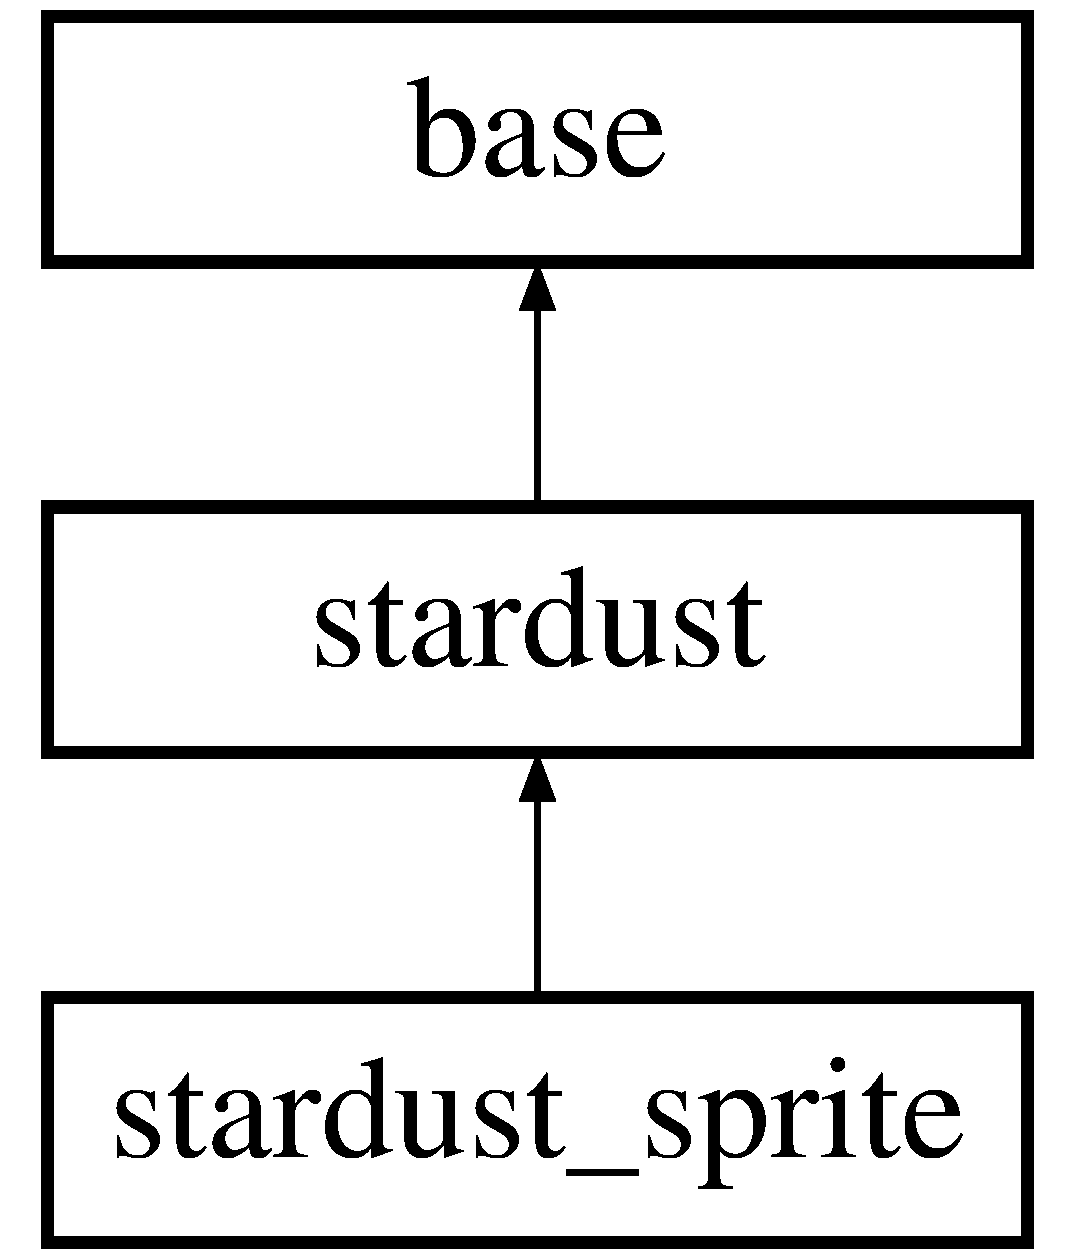
\includegraphics[height=3.000000cm]{classstardust}
\end{center}
\end{figure}
\subsection*{Public Member Functions}
\begin{DoxyCompactItemize}
\item 
\hyperlink{classstardust_a4d48ae45d2e44771d4d26bab9c43b079}{stardust} (const std\-::array$<$ float, 3 $>$ \&\-\_\-col)
\begin{DoxyCompactList}\small\item\em ctor for the stardust class. \end{DoxyCompactList}\item 
\hyperlink{classstardust_a7258eecfcab3503db967f9791afef7f4}{stardust} (float \-\_\-alpha)
\begin{DoxyCompactList}\small\item\em ctor for the stardust class. \end{DoxyCompactList}\item 
void \hyperlink{classstardust_a6c3121d6ef68b5d39ef2cafeb88d8c46}{gen} (bool \-\_\-regen, const std\-::array$<$ float, 3 $>$ \&\-\_\-col)
\begin{DoxyCompactList}\small\item\em Rather than deleting/creating stardust when it goes of screen, we call \hyperlink{classstardust_a6c3121d6ef68b5d39ef2cafeb88d8c46}{gen()} which randomises its member data. \end{DoxyCompactList}\item 
void \hyperlink{classstardust_ac7d44d75f6f9f12b1c75fc17ad543c38}{update\-Pos} (float \-\_\-dt)
\begin{DoxyCompactList}\small\item\em This is a slightly altered update\-Pos function. Since S\-D\-L is 2d, the position increment is based in part off of the z depth. \end{DoxyCompactList}\item 
\hypertarget{classstardust_a5e74804e887f4d73304eb010b572afa3}{void \hyperlink{classstardust_a5e74804e887f4d73304eb010b572afa3}{set\-Z} (float \-\_\-z)}\label{classstardust_a5e74804e887f4d73304eb010b572afa3}

\begin{DoxyCompactList}\small\item\em Setter and getter for z-\/depth. \end{DoxyCompactList}\item 
\hypertarget{classstardust_a99e985c2828dd44f73b8b2043d6f2d75}{float {\bfseries get\-Z} ()}\label{classstardust_a99e985c2828dd44f73b8b2043d6f2d75}

\item 
\hypertarget{classstardust_aee14d29e161fdd8c3cee1d24b29dcabd}{float \hyperlink{classstardust_aee14d29e161fdd8c3cee1d24b29dcabd}{get\-Col} (int \-\_\-i)}\label{classstardust_aee14d29e161fdd8c3cee1d24b29dcabd}

\begin{DoxyCompactList}\small\item\em Getter and setter for the colour. \end{DoxyCompactList}\item 
\hypertarget{classstardust_a5188397b6c9839a70841b4bb891b0ff3}{void {\bfseries set\-Col} (int \-\_\-i, float \-\_\-v)}\label{classstardust_a5188397b6c9839a70841b4bb891b0ff3}

\end{DoxyCompactItemize}


\subsection{Detailed Description}
Legacy class, used in the S\-D\-L renderer only (although a descendant is used by the opengl renderer). 

\subsection{Constructor \& Destructor Documentation}
\hypertarget{classstardust_a4d48ae45d2e44771d4d26bab9c43b079}{\index{stardust@{stardust}!stardust@{stardust}}
\index{stardust@{stardust}!stardust@{stardust}}
\subsubsection[{stardust}]{\setlength{\rightskip}{0pt plus 5cm}stardust\-::stardust (
\begin{DoxyParamCaption}
\item[{const std\-::array$<$ float, 3 $>$ \&}]{\-\_\-col}
\end{DoxyParamCaption}
)}}\label{classstardust_a4d48ae45d2e44771d4d26bab9c43b079}


ctor for the stardust class. 


\begin{DoxyParams}{Parameters}
{\em \-\_\-col} & The colour for the stardust. \\
\hline
\end{DoxyParams}
\hypertarget{classstardust_a7258eecfcab3503db967f9791afef7f4}{\index{stardust@{stardust}!stardust@{stardust}}
\index{stardust@{stardust}!stardust@{stardust}}
\subsubsection[{stardust}]{\setlength{\rightskip}{0pt plus 5cm}stardust\-::stardust (
\begin{DoxyParamCaption}
\item[{float}]{\-\_\-alpha}
\end{DoxyParamCaption}
)}}\label{classstardust_a7258eecfcab3503db967f9791afef7f4}


ctor for the stardust class. 


\begin{DoxyParams}{Parameters}
{\em \-\_\-alpha} & Alpha value of the stardust. \\
\hline
\end{DoxyParams}


\subsection{Member Function Documentation}
\hypertarget{classstardust_a6c3121d6ef68b5d39ef2cafeb88d8c46}{\index{stardust@{stardust}!gen@{gen}}
\index{gen@{gen}!stardust@{stardust}}
\subsubsection[{gen}]{\setlength{\rightskip}{0pt plus 5cm}void stardust\-::gen (
\begin{DoxyParamCaption}
\item[{bool}]{\-\_\-regen, }
\item[{const std\-::array$<$ float, 3 $>$ \&}]{\-\_\-col}
\end{DoxyParamCaption}
)}}\label{classstardust_a6c3121d6ef68b5d39ef2cafeb88d8c46}


Rather than deleting/creating stardust when it goes of screen, we call \hyperlink{classstardust_a6c3121d6ef68b5d39ef2cafeb88d8c46}{gen()} which randomises its member data. 


\begin{DoxyParams}{Parameters}
{\em \-\_\-regen} & Whether the stardust is regenerating or if this is the initial generation \\
\hline
{\em \-\_\-col} & Colour of the stardust. \\
\hline
\end{DoxyParams}
\hypertarget{classstardust_ac7d44d75f6f9f12b1c75fc17ad543c38}{\index{stardust@{stardust}!update\-Pos@{update\-Pos}}
\index{update\-Pos@{update\-Pos}!stardust@{stardust}}
\subsubsection[{update\-Pos}]{\setlength{\rightskip}{0pt plus 5cm}void stardust\-::update\-Pos (
\begin{DoxyParamCaption}
\item[{float}]{\-\_\-dt}
\end{DoxyParamCaption}
)}}\label{classstardust_ac7d44d75f6f9f12b1c75fc17ad543c38}


This is a slightly altered update\-Pos function. Since S\-D\-L is 2d, the position increment is based in part off of the z depth. 


\begin{DoxyParams}{Parameters}
{\em \-\_\-dt} & Time difference. \\
\hline
\end{DoxyParams}


The documentation for this class was generated from the following files\-:\begin{DoxyCompactItemize}
\item 
include/\hyperlink{stardust_8hpp}{stardust.\-hpp}\item 
src/stardust.\-cpp\end{DoxyCompactItemize}

\hypertarget{classstardust__sprite}{\section{stardust\-\_\-sprite Class Reference}
\label{classstardust__sprite}\index{stardust\-\_\-sprite@{stardust\-\_\-sprite}}
}
Inheritance diagram for stardust\-\_\-sprite\-:\begin{figure}[H]
\begin{center}
\leavevmode
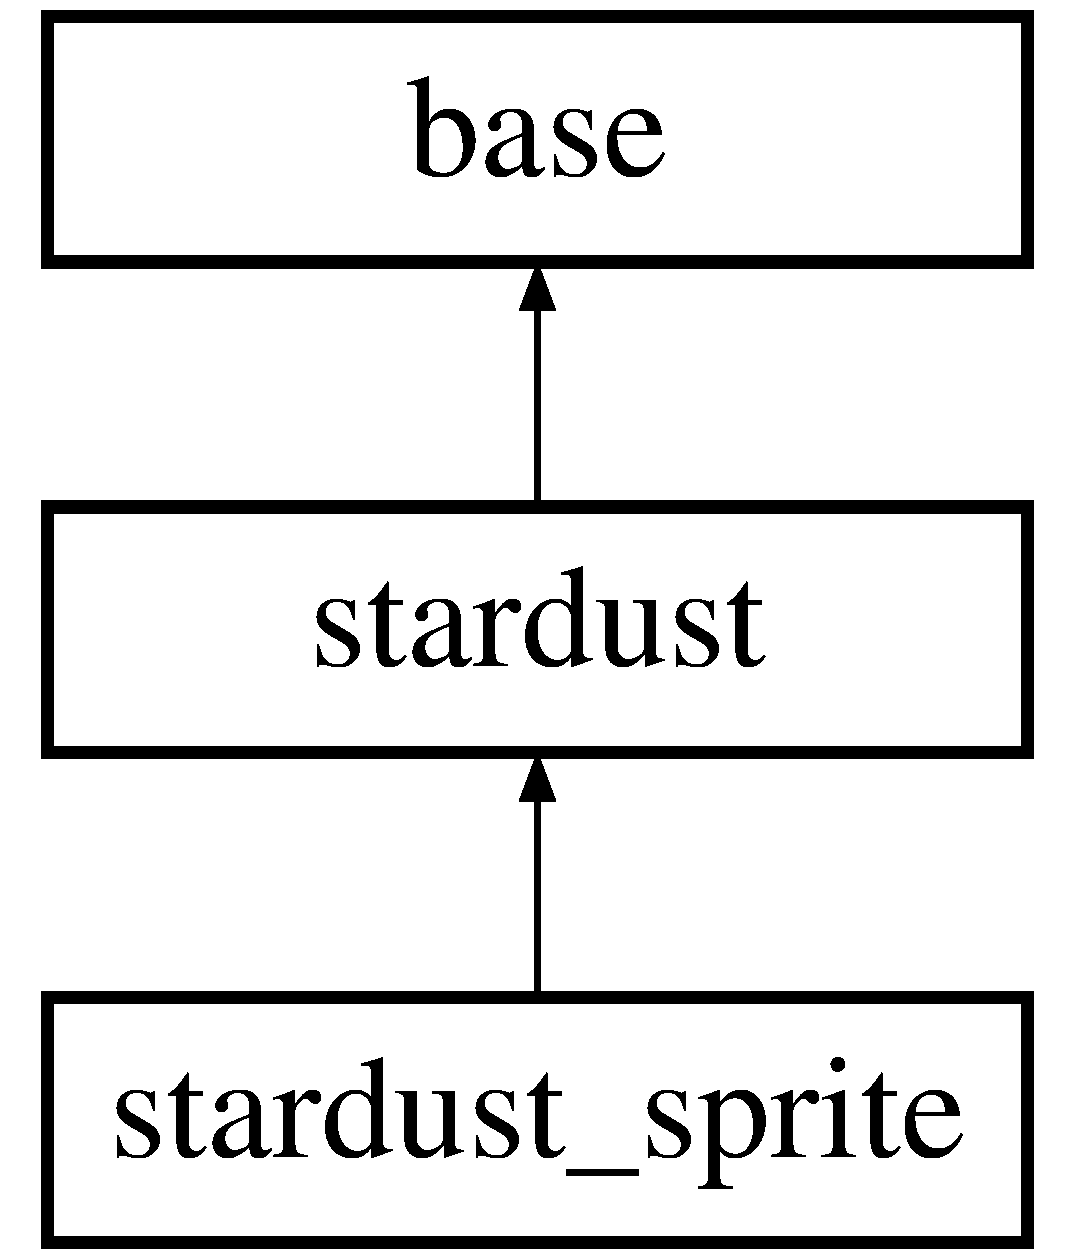
\includegraphics[height=3.000000cm]{classstardust__sprite}
\end{center}
\end{figure}
\subsection*{Public Member Functions}
\begin{DoxyCompactItemize}
\item 
\hyperlink{classstardust__sprite_ab931e35702a0d009841a34586a11c8e9}{stardust\-\_\-sprite} (const std\-::string \-\_\-identifier, const std\-::array$<$ float, 3 $>$ \-\_\-col, const int \-\_\-w, const int \-\_\-h)
\begin{DoxyCompactList}\small\item\em ctor for the \hyperlink{classstardust__sprite}{stardust\-\_\-sprite} class. \end{DoxyCompactList}\item 
\hyperlink{classstardust__sprite_ad89c28faf9b6428504d8f795404f8906}{stardust\-\_\-sprite} (const std\-::string \-\_\-identifier, const float \-\_\-alph, const int \-\_\-w, const int \-\_\-h)
\begin{DoxyCompactList}\small\item\em ctor for the \hyperlink{classstardust__sprite}{stardust\-\_\-sprite} class. \end{DoxyCompactList}\item 
void \hyperlink{classstardust__sprite_af6e688ac14b830357b947952a6bd402e}{sprite\-Gen} (const std\-::array$<$ float, 3 $>$ \&\-\_\-col, const int \-\_\-w, const int \-\_\-h)
\begin{DoxyCompactList}\small\item\em Regenerates stardust sprite attributes. \end{DoxyCompactList}\item 
void \hyperlink{classstardust__sprite_a1b146645cfd0dce69e7053312212e71d}{update\-Sprite} (const float \-\_\-dt)
\begin{DoxyCompactList}\small\item\em Updates the sprite. \end{DoxyCompactList}\item 
void \hyperlink{classstardust__sprite_a7841c172e26158cd108dc48a0ebda755}{incr\-Dim} (float \-\_\-dt)
\begin{DoxyCompactList}\small\item\em Updates the sprite dimensions. \end{DoxyCompactList}\item 
\hypertarget{classstardust__sprite_a3a41460abf840fe0f1b5b9ebacc1df1d}{float \hyperlink{classstardust__sprite_a3a41460abf840fe0f1b5b9ebacc1df1d}{get\-Dim} () const }\label{classstardust__sprite_a3a41460abf840fe0f1b5b9ebacc1df1d}

\begin{DoxyCompactList}\small\item\em Getter for dimensions. \end{DoxyCompactList}\item 
\hypertarget{classstardust__sprite_a89b68b2048f90bc899913d689ed54568}{float \hyperlink{classstardust__sprite_a89b68b2048f90bc899913d689ed54568}{get\-Ang} () const }\label{classstardust__sprite_a89b68b2048f90bc899913d689ed54568}

\begin{DoxyCompactList}\small\item\em Getter for angle. \end{DoxyCompactList}\item 
\hypertarget{classstardust__sprite_a585506ab376a5790e0a8b24f4c95d669}{std\-::string \hyperlink{classstardust__sprite_a585506ab376a5790e0a8b24f4c95d669}{get\-Identifier} ()}\label{classstardust__sprite_a585506ab376a5790e0a8b24f4c95d669}

\begin{DoxyCompactList}\small\item\em Getter for texture identifier. \end{DoxyCompactList}\end{DoxyCompactItemize}


\subsection{Constructor \& Destructor Documentation}
\hypertarget{classstardust__sprite_ab931e35702a0d009841a34586a11c8e9}{\index{stardust\-\_\-sprite@{stardust\-\_\-sprite}!stardust\-\_\-sprite@{stardust\-\_\-sprite}}
\index{stardust\-\_\-sprite@{stardust\-\_\-sprite}!stardust_sprite@{stardust\-\_\-sprite}}
\subsubsection[{stardust\-\_\-sprite}]{\setlength{\rightskip}{0pt plus 5cm}stardust\-\_\-sprite\-::stardust\-\_\-sprite (
\begin{DoxyParamCaption}
\item[{const std\-::string}]{\-\_\-identifier, }
\item[{const std\-::array$<$ float, 3 $>$}]{\-\_\-col, }
\item[{const int}]{\-\_\-w, }
\item[{const int}]{\-\_\-h}
\end{DoxyParamCaption}
)}}\label{classstardust__sprite_ab931e35702a0d009841a34586a11c8e9}


ctor for the \hyperlink{classstardust__sprite}{stardust\-\_\-sprite} class. 


\begin{DoxyParams}{Parameters}
{\em \-\_\-identifier} & string identifier for the sprite \\
\hline
{\em \-\_\-col} & colour of the sprite \\
\hline
{\em \-\_\-w} & width of the sprite \\
\hline
{\em \-\_\-h} & height of the sprite \\
\hline
\end{DoxyParams}
\hypertarget{classstardust__sprite_ad89c28faf9b6428504d8f795404f8906}{\index{stardust\-\_\-sprite@{stardust\-\_\-sprite}!stardust\-\_\-sprite@{stardust\-\_\-sprite}}
\index{stardust\-\_\-sprite@{stardust\-\_\-sprite}!stardust_sprite@{stardust\-\_\-sprite}}
\subsubsection[{stardust\-\_\-sprite}]{\setlength{\rightskip}{0pt plus 5cm}stardust\-\_\-sprite\-::stardust\-\_\-sprite (
\begin{DoxyParamCaption}
\item[{const std\-::string}]{\-\_\-identifier, }
\item[{const float}]{\-\_\-alph, }
\item[{const int}]{\-\_\-w, }
\item[{const int}]{\-\_\-h}
\end{DoxyParamCaption}
)}}\label{classstardust__sprite_ad89c28faf9b6428504d8f795404f8906}


ctor for the \hyperlink{classstardust__sprite}{stardust\-\_\-sprite} class. 


\begin{DoxyParams}{Parameters}
{\em \-\_\-identifier} & string identifier for the sprite \\
\hline
{\em \-\_\-alph} & alpha of the sprite \\
\hline
{\em \-\_\-w} & width of the sprite \\
\hline
{\em \-\_\-h} & height of the sprite \\
\hline
\end{DoxyParams}


\subsection{Member Function Documentation}
\hypertarget{classstardust__sprite_a7841c172e26158cd108dc48a0ebda755}{\index{stardust\-\_\-sprite@{stardust\-\_\-sprite}!incr\-Dim@{incr\-Dim}}
\index{incr\-Dim@{incr\-Dim}!stardust_sprite@{stardust\-\_\-sprite}}
\subsubsection[{incr\-Dim}]{\setlength{\rightskip}{0pt plus 5cm}void stardust\-\_\-sprite\-::incr\-Dim (
\begin{DoxyParamCaption}
\item[{float}]{\-\_\-dt}
\end{DoxyParamCaption}
)}}\label{classstardust__sprite_a7841c172e26158cd108dc48a0ebda755}


Updates the sprite dimensions. 


\begin{DoxyParams}{Parameters}
{\em \-\_\-dt} & timestep \\
\hline
\end{DoxyParams}
\hypertarget{classstardust__sprite_af6e688ac14b830357b947952a6bd402e}{\index{stardust\-\_\-sprite@{stardust\-\_\-sprite}!sprite\-Gen@{sprite\-Gen}}
\index{sprite\-Gen@{sprite\-Gen}!stardust_sprite@{stardust\-\_\-sprite}}
\subsubsection[{sprite\-Gen}]{\setlength{\rightskip}{0pt plus 5cm}void stardust\-\_\-sprite\-::sprite\-Gen (
\begin{DoxyParamCaption}
\item[{const std\-::array$<$ float, 3 $>$ \&}]{\-\_\-col, }
\item[{const int}]{\-\_\-w, }
\item[{const int}]{\-\_\-h}
\end{DoxyParamCaption}
)}}\label{classstardust__sprite_af6e688ac14b830357b947952a6bd402e}


Regenerates stardust sprite attributes. 


\begin{DoxyParams}{Parameters}
{\em \-\_\-col} & colour of the sprite \\
\hline
{\em \-\_\-w} & width of the sprite \\
\hline
{\em \-\_\-h} & height of the sprite \\
\hline
\end{DoxyParams}
\hypertarget{classstardust__sprite_a1b146645cfd0dce69e7053312212e71d}{\index{stardust\-\_\-sprite@{stardust\-\_\-sprite}!update\-Sprite@{update\-Sprite}}
\index{update\-Sprite@{update\-Sprite}!stardust_sprite@{stardust\-\_\-sprite}}
\subsubsection[{update\-Sprite}]{\setlength{\rightskip}{0pt plus 5cm}void stardust\-\_\-sprite\-::update\-Sprite (
\begin{DoxyParamCaption}
\item[{const float}]{\-\_\-dt}
\end{DoxyParamCaption}
)}}\label{classstardust__sprite_a1b146645cfd0dce69e7053312212e71d}


Updates the sprite. 


\begin{DoxyParams}{Parameters}
{\em \-\_\-dt} & timestep \\
\hline
\end{DoxyParams}


The documentation for this class was generated from the following files\-:\begin{DoxyCompactItemize}
\item 
include/stardust\-\_\-sprite.\-hpp\item 
src/stardust\-\_\-sprite.\-cpp\end{DoxyCompactItemize}

\hypertarget{structtinfo}{\section{tinfo Struct Reference}
\label{structtinfo}\index{tinfo@{tinfo}}
}


Contains the dimensions for each ship, based off of its texture.  




{\ttfamily \#include $<$ship.\-hpp$>$}

\subsection*{Public Attributes}
\begin{DoxyCompactItemize}
\item 
\hypertarget{structtinfo_a739a47e942419a16cd995d835401c202}{std\-::string \hyperlink{structtinfo_a739a47e942419a16cd995d835401c202}{m\-\_\-name}}\label{structtinfo_a739a47e942419a16cd995d835401c202}

\begin{DoxyCompactList}\small\item\em The identifier, matches up with a texture id stored in the renderer. \end{DoxyCompactList}\item 
\hypertarget{structtinfo_a98fc4ccb9b63c90cc73d4f66ba7868f0}{float \hyperlink{structtinfo_a98fc4ccb9b63c90cc73d4f66ba7868f0}{m\-\_\-radius}}\label{structtinfo_a98fc4ccb9b63c90cc73d4f66ba7868f0}

\begin{DoxyCompactList}\small\item\em The radius of said texture. \end{DoxyCompactList}\end{DoxyCompactItemize}


\subsection{Detailed Description}
Contains the dimensions for each ship, based off of its texture. 

The documentation for this struct was generated from the following file\-:\begin{DoxyCompactItemize}
\item 
include/\hyperlink{ship_8hpp}{ship.\-hpp}\end{DoxyCompactItemize}

\hypertarget{classuniverse}{\section{universe Class Reference}
\label{classuniverse}\index{universe@{universe}}
}


This class is huge, and touches almost every part of the game.  




{\ttfamily \#include $<$universe.\-hpp$>$}

\subsection*{Public Member Functions}
\begin{DoxyCompactItemize}
\item 
\hypertarget{classuniverse_a53128b9e55c9bb4aff9b0a767db376ef}{\hyperlink{classuniverse_a53128b9e55c9bb4aff9b0a767db376ef}{universe} ()}\label{classuniverse_a53128b9e55c9bb4aff9b0a767db376ef}

\begin{DoxyCompactList}\small\item\em ctor for the universe class, sets up the game and all rendering functionality. \end{DoxyCompactList}\item 
\hypertarget{classuniverse_ac2990f82203890ee22f9a9de1aaec7a1}{void \hyperlink{classuniverse_ac2990f82203890ee22f9a9de1aaec7a1}{init\-U\-I} ()}\label{classuniverse_ac2990f82203890ee22f9a9de1aaec7a1}

\begin{DoxyCompactList}\small\item\em Initialises the U\-I to default values. \end{DoxyCompactList}\item 
\hypertarget{classuniverse_a2f8a7a121a0f933d32789606144d8916}{\hyperlink{classplayer}{player} $\ast$ \hyperlink{classuniverse_a2f8a7a121a0f933d32789606144d8916}{get\-Ply} ()}\label{classuniverse_a2f8a7a121a0f933d32789606144d8916}

\begin{DoxyCompactList}\small\item\em Getter for the player. \end{DoxyCompactList}\item 
\hypertarget{classuniverse_a2e9b69d19436492db80f60a15850b26e}{void \hyperlink{classuniverse_a2e9b69d19436492db80f60a15850b26e}{set\-Vel} (const \hyperlink{structvec3}{vec3} \-\_\-v)}\label{classuniverse_a2e9b69d19436492db80f60a15850b26e}

\begin{DoxyCompactList}\small\item\em Velocity setter. \end{DoxyCompactList}\item 
void \hyperlink{classuniverse_aca6b40fadb1c8390469e6422d61b4c1c}{add\-Shot} (const \hyperlink{structvec3}{vec3} \-\_\-p, const \hyperlink{structvec3}{vec3} \-\_\-v, const float \-\_\-angle, const std\-::array$<$ float, W\-E\-A\-P\-S\-\_\-\-W $>$ \-\_\-weap, const \hyperlink{enemy_8hpp_abac1fdbabb5a6be5f0d6ae40be5c5a58}{ai\-Team} \-\_\-team)
\begin{DoxyCompactList}\small\item\em Adds a laser to the universe. \end{DoxyCompactList}\item 
void \hyperlink{classuniverse_a84c5bf8acb410c81173e0de687fb8672}{add\-Missile} (const \hyperlink{structvec3}{vec3} \-\_\-p, const \hyperlink{structvec3}{vec3} \-\_\-v, const float \-\_\-angle, const \hyperlink{enemy_8hpp_abac1fdbabb5a6be5f0d6ae40be5c5a58}{ai\-Team} \-\_\-team)
\begin{DoxyCompactList}\small\item\em Adds a missile to the universe. \end{DoxyCompactList}\item 
void \hyperlink{classuniverse_afcfa317aadb3a1477e76e2fd8caff1e7}{spawn\-Ship} (const \hyperlink{enemy_8hpp_abac1fdbabb5a6be5f0d6ae40be5c5a58}{ai\-Team} \-\_\-t)
\begin{DoxyCompactList}\small\item\em Adds a ship to the universe, with a random faction and type. \end{DoxyCompactList}\item 
void \hyperlink{classuniverse_a74264fec3d84faf13ab70248be7469c5}{spawn\-Ship} (const \hyperlink{ship_8hpp_af74a63841701826d661cb9809aaf7092}{ship\-\_\-spec} \-\_\-type, const \hyperlink{enemy_8hpp_abac1fdbabb5a6be5f0d6ae40be5c5a58}{ai\-Team} \-\_\-t, const \hyperlink{structvec3}{vec3} \-\_\-p)
\begin{DoxyCompactList}\small\item\em Adds a ship to the universe, with a specified position and type. \end{DoxyCompactList}\item 
\hyperlink{ship_8hpp_af74a63841701826d661cb9809aaf7092}{ship\-\_\-spec} \hyperlink{classuniverse_ad711d97b18ae3f9e35535bf04dd3b0af}{get\-Random\-Ship\-Type} (const \hyperlink{enemy_8hpp_abac1fdbabb5a6be5f0d6ae40be5c5a58}{ai\-Team} \-\_\-t)
\begin{DoxyCompactList}\small\item\em Returns a (weighted) random ship type from a given faction. \end{DoxyCompactList}\item 
void \hyperlink{classuniverse_a4da6321942cd454ac4cadc8d3ccb1740}{spawn\-Squad} (const \hyperlink{enemy_8hpp_abac1fdbabb5a6be5f0d6ae40be5c5a58}{ai\-Team} \-\_\-t, const float \-\_\-min, const float \-\_\-max, const int \-\_\-i)
\begin{DoxyCompactList}\small\item\em Spawns a series of ships. \end{DoxyCompactList}\item 
\hypertarget{classuniverse_aacf31e60bd0e853b488e6a757e1c5c0a}{void \hyperlink{classuniverse_aacf31e60bd0e853b488e6a757e1c5c0a}{add\-Wingman} ()}\label{classuniverse_aacf31e60bd0e853b488e6a757e1c5c0a}

\begin{DoxyCompactList}\small\item\em This function only actually incremements the max number of wingmen available, which are randomly spawned into the scene in the update function. \end{DoxyCompactList}\item 
\hypertarget{classuniverse_af7fcdf7e564fbeabf2e48e698dfc1aad}{void \hyperlink{classuniverse_af7fcdf7e564fbeabf2e48e698dfc1aad}{add\-Miner} ()}\label{classuniverse_af7fcdf7e564fbeabf2e48e698dfc1aad}

\begin{DoxyCompactList}\small\item\em This function only actually incremements the max number of miners available, which are randomly spawned into the scene in the update function. \end{DoxyCompactList}\item 
void \hyperlink{classuniverse_ad058c50da21f46d2eecb276254b79fb1}{add\-Build} (const \hyperlink{structvec3}{vec3} \-\_\-p, const \hyperlink{ship_8hpp_af74a63841701826d661cb9809aaf7092}{ship\-\_\-spec} \-\_\-type)
\begin{DoxyCompactList}\small\item\em Used to place static structures into the world, although under the hood it just spawns a ship with a given classification. \end{DoxyCompactList}\item 
void \hyperlink{classuniverse_aa7edd0f87d1ec40806203444edf84614}{add\-Build} (const \hyperlink{ship_8hpp_af74a63841701826d661cb9809aaf7092}{ship\-\_\-spec} \-\_\-type)
\begin{DoxyCompactList}\small\item\em Used to place static structures in random places. Could be useful for spawning enemy space stations in the future. \end{DoxyCompactList}\item 
void \hyperlink{classuniverse_a3b08f92bb3489f1181d2e8efd5346a56}{update} (const float \-\_\-dt)
\begin{DoxyCompactList}\small\item\em Updates the universe by a given timestep. Physics/\-A\-I and rendering is decoupled, so this may be called multiple times in between each draw-\/call. \end{DoxyCompactList}\item 
\hypertarget{classuniverse_a7a1e6c6398b6a51e5e86e1f31efbb895}{void \hyperlink{classuniverse_a7a1e6c6398b6a51e5e86e1f31efbb895}{clear} ()}\label{classuniverse_a7a1e6c6398b6a51e5e86e1f31efbb895}

\begin{DoxyCompactList}\small\item\em Clears the renderer. \end{DoxyCompactList}\item 
void \hyperlink{classuniverse_a12f3e6d74426ea1165947ec072995eeb}{draw} (const float \-\_\-dt)
\begin{DoxyCompactList}\small\item\em Draws the universe to the screen. \end{DoxyCompactList}\item 
\hypertarget{classuniverse_a2c7ae3efb623c29b37154726127c2d64}{void \hyperlink{classuniverse_a2c7ae3efb623c29b37154726127c2d64}{draw\-U\-I} ()}\label{classuniverse_a2c7ae3efb623c29b37154726127c2d64}

\begin{DoxyCompactList}\small\item\em Draws the user interface to the screen. Does not handle user input. \end{DoxyCompactList}\item 
\hypertarget{classuniverse_a62ca92c3e40069cbf3a411c1a4a696b1}{void \hyperlink{classuniverse_a62ca92c3e40069cbf3a411c1a4a696b1}{swap} ()}\label{classuniverse_a62ca92c3e40069cbf3a411c1a4a696b1}

\begin{DoxyCompactList}\small\item\em Updates the renderer. \end{DoxyCompactList}\item 
void \hyperlink{classuniverse_afd96a7a54d67a2f87a6c4542fb974f53}{detect\-Collisions} (const S\-D\-L\-\_\-\-Rect \-\_\-box, std\-::vector$<$ \hyperlink{classenemy}{enemy} $\ast$ $>$ \-\_\-ships, std\-::vector$<$ \hyperlink{classlaser}{laser} $\ast$ $>$ \-\_\-lasers, std\-::vector$<$ \hyperlink{classmissile}{missile} $\ast$ $>$ \-\_\-rockets, std\-::vector$<$ \hyperlink{classship}{ship} $\ast$ $>$ \-\_\-rocks, unsigned short int \-\_\-lvl)
\begin{DoxyCompactList}\small\item\em \hyperlink{struct_a}{A} broad phase, this is used to detect entities which are close to one another. \end{DoxyCompactList}\item 
\hypertarget{classuniverse_a5ca840e2d9777dd97867d360ae4d089f}{void \hyperlink{classuniverse_a5ca840e2d9777dd97867d360ae4d089f}{check\-Collisions} ()}\label{classuniverse_a5ca840e2d9777dd97867d360ae4d089f}

\begin{DoxyCompactList}\small\item\em \hyperlink{struct_a}{A} narrow phase, this checks through the partitioned entities in detail. \end{DoxyCompactList}\item 
void \hyperlink{classuniverse_a76efbef30d81b0893bbefbbb95697696}{addpfx} (const \hyperlink{structvec3}{vec3} \-\_\-p, const \hyperlink{structvec3}{vec3} \-\_\-v, const \hyperlink{structvec3}{vec3} \-\_\-wv, const int \-\_\-no, const float \-\_\-f)
\begin{DoxyCompactList}\small\item\em Adds a particle system to the universe. \end{DoxyCompactList}\item 
void \hyperlink{classuniverse_a1b868fe830fa921552b8d852ed74db1d}{add\-Particle\-Sprite} (const \hyperlink{structvec3}{vec3} \-\_\-p, const \hyperlink{structvec3}{vec3} \-\_\-v, const std\-::string \-\_\-tex)
\begin{DoxyCompactList}\small\item\em Adds a particle sprite to the universe. This is a bit of a misnomer, since the opengl renderer uses billboards + glsl. \end{DoxyCompactList}\item 
\hypertarget{classuniverse_a4e6b1f07fdd28f8308499015855ddead}{std\-::vector$<$ \hyperlink{classenemy}{enemy} $>$ $\ast$ \hyperlink{classuniverse_a4e6b1f07fdd28f8308499015855ddead}{get\-Agents} ()}\label{classuniverse_a4e6b1f07fdd28f8308499015855ddead}

\begin{DoxyCompactList}\small\item\em Gets a pointer to the agents vector. Mostly a quick and dirty way of doing stuff in the tutorial, and for file operations. \end{DoxyCompactList}\item 
\hypertarget{classuniverse_ab93032a40b560a5059aa404450d08b20}{std\-::vector$<$ \hyperlink{classlaser}{laser} $>$ $\ast$ \hyperlink{classuniverse_ab93032a40b560a5059aa404450d08b20}{get\-Shots} ()}\label{classuniverse_ab93032a40b560a5059aa404450d08b20}

\begin{DoxyCompactList}\small\item\em Gets a pointer to the laser vector. Mostly used for saving and loading the game. \end{DoxyCompactList}\item 
\hypertarget{classuniverse_ab2639f597a44279b69fec654b2790f1f}{std\-::vector$<$ \hyperlink{classmissile}{missile} $>$ $\ast$ \hyperlink{classuniverse_ab2639f597a44279b69fec654b2790f1f}{get\-Missiles} ()}\label{classuniverse_ab2639f597a44279b69fec654b2790f1f}

\begin{DoxyCompactList}\small\item\em Gets a pointer to the missile vector. Mostly used for saving and loading the game. \end{DoxyCompactList}\item 
\hypertarget{classuniverse_af16581985c050c653eac9381d619f4b8}{std\-::vector$<$ \hyperlink{classship}{ship} $>$ $\ast$ \hyperlink{classuniverse_af16581985c050c653eac9381d619f4b8}{get\-Asteroids} ()}\label{classuniverse_af16581985c050c653eac9381d619f4b8}

\begin{DoxyCompactList}\small\item\em Gets a pointer to the asteroid vector. Mostly used for saving and loading the game. \end{DoxyCompactList}\item 
\hyperlink{classship}{ship} $\ast$ \hyperlink{classuniverse_a62c18e794bc3f09e1a724b8588ee46a4}{closest\-Enemy} (const \hyperlink{structvec3}{vec3} \-\_\-p, const \hyperlink{enemy_8hpp_abac1fdbabb5a6be5f0d6ae40be5c5a58}{ai\-Team} \-\_\-t)
\begin{DoxyCompactList}\small\item\em Gets the closest enemy to a given point in space, mostly used for missile tracking. \end{DoxyCompactList}\item 
\hypertarget{classuniverse_ab23b66c1edc3f954997475cdc0c9cd4a}{void \hyperlink{classuniverse_ab23b66c1edc3f954997475cdc0c9cd4a}{set\-Score} (const int \-\_\-s)}\label{classuniverse_ab23b66c1edc3f954997475cdc0c9cd4a}

\begin{DoxyCompactList}\small\item\em Getters and setters for the score. \end{DoxyCompactList}\item 
\hypertarget{classuniverse_a6b615a23dcbb9b55c07ed301101b99ea}{void {\bfseries add\-Score} (const int \-\_\-s)}\label{classuniverse_a6b615a23dcbb9b55c07ed301101b99ea}

\item 
\hypertarget{classuniverse_a1d401f812d523ba736f2e2adc858c2e5}{int {\bfseries get\-Score} () const }\label{classuniverse_a1d401f812d523ba736f2e2adc858c2e5}

\item 
\hypertarget{classuniverse_a8b31cce5565fdd692fdbb476c6e54257}{int $\ast$ {\bfseries get\-Score\-Pt} ()}\label{classuniverse_a8b31cce5565fdd692fdbb476c6e54257}

\item 
\hypertarget{classuniverse_a618ef9595ad161031dacb3909a694330}{int \hyperlink{classuniverse_a618ef9595ad161031dacb3909a694330}{get\-Max\-Enemy\-Count} (\hyperlink{enemy_8hpp_abac1fdbabb5a6be5f0d6ae40be5c5a58}{ai\-Team} \-\_\-t) const }\label{classuniverse_a618ef9595ad161031dacb3909a694330}

\begin{DoxyCompactList}\small\item\em Getter and setter for the max enemy count. \end{DoxyCompactList}\item 
\hypertarget{classuniverse_a70b6a09e9fa7a93b65f1d6182f86181e}{void {\bfseries set\-Max\-Enemy\-Count} (const int m, const \hyperlink{enemy_8hpp_abac1fdbabb5a6be5f0d6ae40be5c5a58}{ai\-Team} \-\_\-t)}\label{classuniverse_a70b6a09e9fa7a93b65f1d6182f86181e}

\item 
\hypertarget{classuniverse_a02a9b87c10d761ba90bddcba429c8840}{int \hyperlink{classuniverse_a02a9b87c10d761ba90bddcba429c8840}{get\-Enemy\-Count} (\hyperlink{enemy_8hpp_abac1fdbabb5a6be5f0d6ae40be5c5a58}{ai\-Team} \-\_\-t) const }\label{classuniverse_a02a9b87c10d761ba90bddcba429c8840}

\begin{DoxyCompactList}\small\item\em Getter for the enemy count. \end{DoxyCompactList}\item 
\hypertarget{classuniverse_a2f92ca94b16cb4734cc51b673488cd0d}{int \hyperlink{classuniverse_a2f92ca94b16cb4734cc51b673488cd0d}{get\-Max\-Wingman\-Count} () const }\label{classuniverse_a2f92ca94b16cb4734cc51b673488cd0d}

\begin{DoxyCompactList}\small\item\em Getter for the max wingman count. \end{DoxyCompactList}\item 
\hypertarget{classuniverse_a200ab28e86c28228088919c3e667d90d}{void {\bfseries set\-Max\-Wingman\-Count} (const int m)}\label{classuniverse_a200ab28e86c28228088919c3e667d90d}

\item 
\hypertarget{classuniverse_a6889a4cb6b8aaecd6c8abe363c8a80ec}{int \hyperlink{classuniverse_a6889a4cb6b8aaecd6c8abe363c8a80ec}{get\-Max\-Miner\-Count} () const }\label{classuniverse_a6889a4cb6b8aaecd6c8abe363c8a80ec}

\begin{DoxyCompactList}\small\item\em Getter for the max miner count. \end{DoxyCompactList}\item 
\hypertarget{classuniverse_a7e45dbd5f966aec0b90ba9d122586637}{void {\bfseries set\-Max\-Miner\-Count} (const int m)}\label{classuniverse_a7e45dbd5f966aec0b90ba9d122586637}

\item 
\hypertarget{classuniverse_aaaca317c6f2a23053c28550580e16d5c}{bool \hyperlink{classuniverse_aaaca317c6f2a23053c28550580e16d5c}{at\-Max\-Count} (\hyperlink{enemy_8hpp_abac1fdbabb5a6be5f0d6ae40be5c5a58}{ai\-Team} \-\_\-t) const }\label{classuniverse_aaaca317c6f2a23053c28550580e16d5c}

\begin{DoxyCompactList}\small\item\em Check to see if a given faction has reached its max count. \end{DoxyCompactList}\item 
void \hyperlink{classuniverse_aa3bb66d17df83723a112dc75cd44fdcc}{reload} (const bool \-\_\-new\-Game)
\begin{DoxyCompactList}\small\item\em Resets the universe, and clears containers. Used to start a new game. \end{DoxyCompactList}\item 
\hypertarget{classuniverse_a7246a93d0a18354e7b35f7f48f595ffa}{void \hyperlink{classuniverse_a7246a93d0a18354e7b35f7f48f595ffa}{load\-Ships} ()}\label{classuniverse_a7246a93d0a18354e7b35f7f48f595ffa}

\begin{DoxyCompactList}\small\item\em Fills g\-\_\-ship\-\_\-templates, which we can copy from later on. \end{DoxyCompactList}\item 
\hypertarget{classuniverse_ac311a26eb9b23ee745e93b94f358e6fb}{void \hyperlink{classuniverse_ac311a26eb9b23ee745e93b94f358e6fb}{pause} ()}\label{classuniverse_ac311a26eb9b23ee745e93b94f358e6fb}

\begin{DoxyCompactList}\small\item\em Getter and setters for game pause. \end{DoxyCompactList}\item 
\hypertarget{classuniverse_a45ec0b47345bb1d4dc324f09100e9286}{void {\bfseries set\-Pause} (bool \-\_\-p)}\label{classuniverse_a45ec0b47345bb1d4dc324f09100e9286}

\item 
\hypertarget{classuniverse_ad5cc400800e499f80e1e7722515bc216}{bool {\bfseries is\-Paused} () const }\label{classuniverse_ad5cc400800e499f80e1e7722515bc216}

\item 
\hypertarget{classuniverse_a65fe9d463d02b0fbed6e1dc28b6657cb}{\hyperlink{classui_1_1user_interface}{ui\-::user\-Interface} $\ast$ \hyperlink{classuniverse_a65fe9d463d02b0fbed6e1dc28b6657cb}{get\-U\-I} ()}\label{classuniverse_a65fe9d463d02b0fbed6e1dc28b6657cb}

\begin{DoxyCompactList}\small\item\em Getter and setter for the U\-I. \end{DoxyCompactList}\item 
\hypertarget{classuniverse_a78ad78159c1e509f091cd0fac62a5fc1}{\hyperlink{classui_1_1user_interface}{ui\-::user\-Interface} {\bfseries set\-U\-I} (\hyperlink{classui_1_1user_interface}{ui\-::user\-Interface} \-\_\-i)}\label{classuniverse_a78ad78159c1e509f091cd0fac62a5fc1}

\item 
bool \hyperlink{classuniverse_a09a2c776eb45b5667e096ff9881c5e77}{upgrade\-Callback} (const int \-\_\-sel, const int \-\_\-btn)
\begin{DoxyCompactList}\small\item\em \hyperlink{struct_a}{A} function to tell whether we are allowed to upgrade (compares cost vs score etc). \end{DoxyCompactList}\item 
\hypertarget{classuniverse_a1c7652330bd49d9f01e9ab32f89d90c9}{void {\bfseries upgrade\-Set\-Labels} (const int \-\_\-sel, const int \-\_\-btn, const int \-\_\-plvl)}\label{classuniverse_a1c7652330bd49d9f01e9ab32f89d90c9}

\item 
\hypertarget{classuniverse_ab2890c3b19620f5bbefbb31fce0774d7}{void \hyperlink{classuniverse_ab2890c3b19620f5bbefbb31fce0774d7}{set\-Mouse\-State} (const int \-\_\-i)}\label{classuniverse_ab2890c3b19620f5bbefbb31fce0774d7}

\begin{DoxyCompactList}\small\item\em Getter and setter for the mouse state. \end{DoxyCompactList}\item 
\hypertarget{classuniverse_a1c4472798eb406c841e46015d1ef418a}{int {\bfseries get\-Mouse\-State} () const }\label{classuniverse_a1c4472798eb406c841e46015d1ef418a}

\item 
void \hyperlink{classuniverse_a5125ff87385bdd80c1e96f302e0594f6}{add\-To\-Squad} (\hyperlink{classenemy}{enemy} $\ast$\-\_\-e, \hyperlink{structsquad}{squad} $\ast$\-\_\-s)
\begin{DoxyCompactList}\small\item\em Adds a given enemy to a given squad. \end{DoxyCompactList}\item 
void \hyperlink{classuniverse_a3af60fa4c1b4e0c691c940f0d9e2af88}{remove\-From\-Squad} (\hyperlink{classenemy}{enemy} $\ast$\-\_\-e, \hyperlink{structsquad}{squad} $\ast$\-\_\-s)
\begin{DoxyCompactList}\small\item\em Removes a given enemy from a given squad. Requires you know which squad it is in. \end{DoxyCompactList}\item 
\hypertarget{classuniverse_ac067d5e3b2a77871d317538d86638078}{void \hyperlink{classuniverse_ac067d5e3b2a77871d317538d86638078}{create\-Factions} ()}\label{classuniverse_ac067d5e3b2a77871d317538d86638078}

\begin{DoxyCompactList}\small\item\em Creates the factions and stores them in m\-\_\-factions. \end{DoxyCompactList}\item 
\hypertarget{classuniverse_a1069edc3188cbb18edc64d73c3f9cce0}{\hyperlink{structsquad}{squad} $\ast$ \hyperlink{classuniverse_a1069edc3188cbb18edc64d73c3f9cce0}{get\-Squad\-From\-I\-D} (int \-\_\-id)}\label{classuniverse_a1069edc3188cbb18edc64d73c3f9cce0}

\begin{DoxyCompactList}\small\item\em Given a squad I\-D, returns the associated squad. \end{DoxyCompactList}\item 
\hypertarget{classuniverse_a510e65884b42bae6d4e5469a476bd9e0}{\hyperlink{classrenderer__ngl}{renderer\-\_\-ngl} $\ast$ \hyperlink{classuniverse_a510e65884b42bae6d4e5469a476bd9e0}{get\-Renderer} ()}\label{classuniverse_a510e65884b42bae6d4e5469a476bd9e0}

\begin{DoxyCompactList}\small\item\em Returns the renderer. Mostly used to hack text into the tutorial. \end{DoxyCompactList}\item 
\hypertarget{classuniverse_a14b80a5ddef84ee3dff40cd2d4a394b3}{bool \hyperlink{classuniverse_a14b80a5ddef84ee3dff40cd2d4a394b3}{is\-Esc\-Menu\-Shown} ()}\label{classuniverse_a14b80a5ddef84ee3dff40cd2d4a394b3}

\begin{DoxyCompactList}\small\item\em Getter and setter for the boolean associated with the in game options menu display. \end{DoxyCompactList}\item 
\hypertarget{classuniverse_a70c60dc136b8466aee31f314bbaa20c8}{void {\bfseries esc\-Menu\-Tog} ()}\label{classuniverse_a70c60dc136b8466aee31f314bbaa20c8}

\item 
\hypertarget{classuniverse_aeac69d5ee3f92bbfd9a66ed9ce41df82}{bool \hyperlink{classuniverse_aeac69d5ee3f92bbfd9a66ed9ce41df82}{U\-I\-Visible} () const }\label{classuniverse_aeac69d5ee3f92bbfd9a66ed9ce41df82}

\begin{DoxyCompactList}\small\item\em Getters and setters for U\-I visibility. \end{DoxyCompactList}\item 
\hypertarget{classuniverse_a096b56203fa8b57e10b7bc7f57eb6861}{void {\bfseries set\-U\-I\-Visible} (const bool \-\_\-b)}\label{classuniverse_a096b56203fa8b57e10b7bc7f57eb6861}

\item 
\hypertarget{classuniverse_a4756c43cd7d9852d1fa1a3b6e241a57c}{void {\bfseries toggle\-U\-I\-Visible} ()}\label{classuniverse_a4756c43cd7d9852d1fa1a3b6e241a57c}

\item 
void \hyperlink{classuniverse_a71dd4cdc7489ee3d8daabf37e3b65e3d}{ship\-Add\-Parent} (\hyperlink{classship}{ship} $\ast$\-\_\-parent, \hyperlink{classship}{ship} $\ast$\-\_\-child, \hyperlink{structvec3}{vec3} \-\_\-offset)
\begin{DoxyCompactList}\small\item\em Gives a ship a parent, and an offset from said parent. \end{DoxyCompactList}\end{DoxyCompactItemize}


\subsection{Detailed Description}
This class is huge, and touches almost every part of the game. 

\subsection{Member Function Documentation}
\hypertarget{classuniverse_ad058c50da21f46d2eecb276254b79fb1}{\index{universe@{universe}!add\-Build@{add\-Build}}
\index{add\-Build@{add\-Build}!universe@{universe}}
\subsubsection[{add\-Build}]{\setlength{\rightskip}{0pt plus 5cm}void universe\-::add\-Build (
\begin{DoxyParamCaption}
\item[{const {\bf vec3}}]{\-\_\-p, }
\item[{const {\bf ship\-\_\-spec}}]{\-\_\-type}
\end{DoxyParamCaption}
)}}\label{classuniverse_ad058c50da21f46d2eecb276254b79fb1}


Used to place static structures into the world, although under the hood it just spawns a ship with a given classification. 


\begin{DoxyParams}{Parameters}
{\em \-\_\-p} & position \\
\hline
{\em \-\_\-type} & ship classification \\
\hline
\end{DoxyParams}
\hypertarget{classuniverse_aa7edd0f87d1ec40806203444edf84614}{\index{universe@{universe}!add\-Build@{add\-Build}}
\index{add\-Build@{add\-Build}!universe@{universe}}
\subsubsection[{add\-Build}]{\setlength{\rightskip}{0pt plus 5cm}void universe\-::add\-Build (
\begin{DoxyParamCaption}
\item[{const {\bf ship\-\_\-spec}}]{\-\_\-type}
\end{DoxyParamCaption}
)}}\label{classuniverse_aa7edd0f87d1ec40806203444edf84614}


Used to place static structures in random places. Could be useful for spawning enemy space stations in the future. 


\begin{DoxyParams}{Parameters}
{\em \-\_\-type} & ship classification. \\
\hline
\end{DoxyParams}
\hypertarget{classuniverse_a84c5bf8acb410c81173e0de687fb8672}{\index{universe@{universe}!add\-Missile@{add\-Missile}}
\index{add\-Missile@{add\-Missile}!universe@{universe}}
\subsubsection[{add\-Missile}]{\setlength{\rightskip}{0pt plus 5cm}void universe\-::add\-Missile (
\begin{DoxyParamCaption}
\item[{const {\bf vec3}}]{\-\_\-p, }
\item[{const {\bf vec3}}]{\-\_\-v, }
\item[{const float}]{\-\_\-angle, }
\item[{const {\bf ai\-Team}}]{\-\_\-team}
\end{DoxyParamCaption}
)}}\label{classuniverse_a84c5bf8acb410c81173e0de687fb8672}


Adds a missile to the universe. 


\begin{DoxyParams}{Parameters}
{\em \-\_\-p} & position \\
\hline
{\em \-\_\-v} & velocity \\
\hline
{\em \-\_\-angle} & initial angle \\
\hline
{\em \-\_\-team} & source of the missile \\
\hline
\end{DoxyParams}
\hypertarget{classuniverse_a1b868fe830fa921552b8d852ed74db1d}{\index{universe@{universe}!add\-Particle\-Sprite@{add\-Particle\-Sprite}}
\index{add\-Particle\-Sprite@{add\-Particle\-Sprite}!universe@{universe}}
\subsubsection[{add\-Particle\-Sprite}]{\setlength{\rightskip}{0pt plus 5cm}void universe\-::add\-Particle\-Sprite (
\begin{DoxyParamCaption}
\item[{const {\bf vec3}}]{\-\_\-p, }
\item[{const {\bf vec3}}]{\-\_\-v, }
\item[{const std\-::string}]{\-\_\-tex}
\end{DoxyParamCaption}
)}}\label{classuniverse_a1b868fe830fa921552b8d852ed74db1d}


Adds a particle sprite to the universe. This is a bit of a misnomer, since the opengl renderer uses billboards + glsl. 


\begin{DoxyParams}{Parameters}
{\em \-\_\-p} & position \\
\hline
{\em \-\_\-v} & velocity \\
\hline
{\em \-\_\-tex} & surface identifier ie \char`\"{}\-S\-M\-O\-K\-E\char`\"{}. \\
\hline
\end{DoxyParams}
\hypertarget{classuniverse_a76efbef30d81b0893bbefbbb95697696}{\index{universe@{universe}!addpfx@{addpfx}}
\index{addpfx@{addpfx}!universe@{universe}}
\subsubsection[{addpfx}]{\setlength{\rightskip}{0pt plus 5cm}void universe\-::addpfx (
\begin{DoxyParamCaption}
\item[{const {\bf vec3}}]{\-\_\-p, }
\item[{const {\bf vec3}}]{\-\_\-v, }
\item[{const {\bf vec3}}]{\-\_\-wv, }
\item[{const int}]{\-\_\-no, }
\item[{const float}]{\-\_\-f}
\end{DoxyParamCaption}
)}}\label{classuniverse_a76efbef30d81b0893bbefbbb95697696}


Adds a particle system to the universe. 


\begin{DoxyParams}{Parameters}
{\em \-\_\-type} & ship classification. \\
\hline
\end{DoxyParams}
\hypertarget{classuniverse_aca6b40fadb1c8390469e6422d61b4c1c}{\index{universe@{universe}!add\-Shot@{add\-Shot}}
\index{add\-Shot@{add\-Shot}!universe@{universe}}
\subsubsection[{add\-Shot}]{\setlength{\rightskip}{0pt plus 5cm}void universe\-::add\-Shot (
\begin{DoxyParamCaption}
\item[{const {\bf vec3}}]{\-\_\-p, }
\item[{const {\bf vec3}}]{\-\_\-v, }
\item[{const float}]{\-\_\-angle, }
\item[{const std\-::array$<$ float, W\-E\-A\-P\-S\-\_\-\-W $>$}]{\-\_\-weap, }
\item[{const {\bf ai\-Team}}]{\-\_\-team}
\end{DoxyParamCaption}
)}}\label{classuniverse_aca6b40fadb1c8390469e6422d61b4c1c}


Adds a laser to the universe. 


\begin{DoxyParams}{Parameters}
{\em \-\_\-p} & position \\
\hline
{\em \-\_\-v} & velocity \\
\hline
{\em \-\_\-angle} & initial angle \\
\hline
{\em \-\_\-weap} & array of data such as damage \\
\hline
{\em \-\_\-team} & source of the shot \\
\hline
\end{DoxyParams}
\hypertarget{classuniverse_a5125ff87385bdd80c1e96f302e0594f6}{\index{universe@{universe}!add\-To\-Squad@{add\-To\-Squad}}
\index{add\-To\-Squad@{add\-To\-Squad}!universe@{universe}}
\subsubsection[{add\-To\-Squad}]{\setlength{\rightskip}{0pt plus 5cm}void universe\-::add\-To\-Squad (
\begin{DoxyParamCaption}
\item[{{\bf enemy} $\ast$}]{\-\_\-e, }
\item[{{\bf squad} $\ast$}]{\-\_\-s}
\end{DoxyParamCaption}
)\hspace{0.3cm}{\ttfamily [inline]}}}\label{classuniverse_a5125ff87385bdd80c1e96f302e0594f6}


Adds a given enemy to a given squad. 


\begin{DoxyParams}{Parameters}
{\em \-\_\-e} & enemy to add \\
\hline
{\em \-\_\-s} & squad to add to \\
\hline
\end{DoxyParams}
\hypertarget{classuniverse_a62c18e794bc3f09e1a724b8588ee46a4}{\index{universe@{universe}!closest\-Enemy@{closest\-Enemy}}
\index{closest\-Enemy@{closest\-Enemy}!universe@{universe}}
\subsubsection[{closest\-Enemy}]{\setlength{\rightskip}{0pt plus 5cm}{\bf ship} $\ast$ universe\-::closest\-Enemy (
\begin{DoxyParamCaption}
\item[{const {\bf vec3}}]{\-\_\-p, }
\item[{const {\bf ai\-Team}}]{\-\_\-t}
\end{DoxyParamCaption}
)}}\label{classuniverse_a62c18e794bc3f09e1a724b8588ee46a4}


Gets the closest enemy to a given point in space, mostly used for missile tracking. 


\begin{DoxyParams}{Parameters}
{\em \-\_\-p} & position \\
\hline
{\em \-\_\-t} & team to check against \\
\hline
\end{DoxyParams}
\hypertarget{classuniverse_afd96a7a54d67a2f87a6c4542fb974f53}{\index{universe@{universe}!detect\-Collisions@{detect\-Collisions}}
\index{detect\-Collisions@{detect\-Collisions}!universe@{universe}}
\subsubsection[{detect\-Collisions}]{\setlength{\rightskip}{0pt plus 5cm}void universe\-::detect\-Collisions (
\begin{DoxyParamCaption}
\item[{const S\-D\-L\-\_\-\-Rect}]{\-\_\-box, }
\item[{std\-::vector$<$ {\bf enemy} $\ast$ $>$}]{\-\_\-ships, }
\item[{std\-::vector$<$ {\bf laser} $\ast$ $>$}]{\-\_\-lasers, }
\item[{std\-::vector$<$ {\bf missile} $\ast$ $>$}]{\-\_\-rockets, }
\item[{std\-::vector$<$ {\bf ship} $\ast$ $>$}]{\-\_\-rocks, }
\item[{unsigned short int}]{\-\_\-lvl}
\end{DoxyParamCaption}
)}}\label{classuniverse_afd96a7a54d67a2f87a6c4542fb974f53}


\hyperlink{struct_a}{A} broad phase, this is used to detect entities which are close to one another. 


\begin{DoxyParams}{Parameters}
{\em \-\_\-box} & Bounding box enclosing the entities to be sorted, \\
\hline
{\em \-\_\-ships} & references to ships to be sorted \\
\hline
{\em \-\_\-lasers} & references to lasers to be sorted \\
\hline
{\em \-\_\-rockets} & references to missiles to be sorted \\
\hline
{\em \-\_\-rocks} & references to asteroids to be sorted \\
\hline
{\em \-\_\-lvl} & current level of recursion \\
\hline
\end{DoxyParams}
\hypertarget{classuniverse_a12f3e6d74426ea1165947ec072995eeb}{\index{universe@{universe}!draw@{draw}}
\index{draw@{draw}!universe@{universe}}
\subsubsection[{draw}]{\setlength{\rightskip}{0pt plus 5cm}void universe\-::draw (
\begin{DoxyParamCaption}
\item[{const float}]{\-\_\-dt}
\end{DoxyParamCaption}
)}}\label{classuniverse_a12f3e6d74426ea1165947ec072995eeb}


Draws the universe to the screen. 


\begin{DoxyParams}{Parameters}
{\em \-\_\-dt} & time difference, we can linearly interpolate objects being drawn to ensure that their movement is continuous. \\
\hline
\end{DoxyParams}
\hypertarget{classuniverse_ad711d97b18ae3f9e35535bf04dd3b0af}{\index{universe@{universe}!get\-Random\-Ship\-Type@{get\-Random\-Ship\-Type}}
\index{get\-Random\-Ship\-Type@{get\-Random\-Ship\-Type}!universe@{universe}}
\subsubsection[{get\-Random\-Ship\-Type}]{\setlength{\rightskip}{0pt plus 5cm}{\bf ship\-\_\-spec} universe\-::get\-Random\-Ship\-Type (
\begin{DoxyParamCaption}
\item[{const {\bf ai\-Team}}]{\-\_\-t}
\end{DoxyParamCaption}
)}}\label{classuniverse_ad711d97b18ae3f9e35535bf04dd3b0af}


Returns a (weighted) random ship type from a given faction. 


\begin{DoxyParams}{Parameters}
{\em \-\_\-t} & ship faction. \\
\hline
\end{DoxyParams}
\hypertarget{classuniverse_aa3bb66d17df83723a112dc75cd44fdcc}{\index{universe@{universe}!reload@{reload}}
\index{reload@{reload}!universe@{universe}}
\subsubsection[{reload}]{\setlength{\rightskip}{0pt plus 5cm}void universe\-::reload (
\begin{DoxyParamCaption}
\item[{const bool}]{\-\_\-new\-Game}
\end{DoxyParamCaption}
)}}\label{classuniverse_aa3bb66d17df83723a112dc75cd44fdcc}


Resets the universe, and clears containers. Used to start a new game. 


\begin{DoxyParams}{Parameters}
{\em \-\_\-new\-Game} & whether we are starting a new game. \\
\hline
\end{DoxyParams}
\hypertarget{classuniverse_a3af60fa4c1b4e0c691c940f0d9e2af88}{\index{universe@{universe}!remove\-From\-Squad@{remove\-From\-Squad}}
\index{remove\-From\-Squad@{remove\-From\-Squad}!universe@{universe}}
\subsubsection[{remove\-From\-Squad}]{\setlength{\rightskip}{0pt plus 5cm}void universe\-::remove\-From\-Squad (
\begin{DoxyParamCaption}
\item[{{\bf enemy} $\ast$}]{\-\_\-e, }
\item[{{\bf squad} $\ast$}]{\-\_\-s}
\end{DoxyParamCaption}
)\hspace{0.3cm}{\ttfamily [inline]}}}\label{classuniverse_a3af60fa4c1b4e0c691c940f0d9e2af88}


Removes a given enemy from a given squad. Requires you know which squad it is in. 


\begin{DoxyParams}{Parameters}
{\em \-\_\-e} & enemy to remove \\
\hline
{\em \-\_\-s} & squad to remove from \\
\hline
\end{DoxyParams}
\hypertarget{classuniverse_a71dd4cdc7489ee3d8daabf37e3b65e3d}{\index{universe@{universe}!ship\-Add\-Parent@{ship\-Add\-Parent}}
\index{ship\-Add\-Parent@{ship\-Add\-Parent}!universe@{universe}}
\subsubsection[{ship\-Add\-Parent}]{\setlength{\rightskip}{0pt plus 5cm}void universe\-::ship\-Add\-Parent (
\begin{DoxyParamCaption}
\item[{{\bf ship} $\ast$}]{\-\_\-parent, }
\item[{{\bf ship} $\ast$}]{\-\_\-child, }
\item[{{\bf vec3}}]{\-\_\-offset}
\end{DoxyParamCaption}
)}}\label{classuniverse_a71dd4cdc7489ee3d8daabf37e3b65e3d}


Gives a ship a parent, and an offset from said parent. 


\begin{DoxyParams}{Parameters}
{\em \-\_\-parent} & parent ship \\
\hline
{\em \-\_\-child} & child ship \\
\hline
{\em \-\_\-offset} & childs offset from the parent \\
\hline
\end{DoxyParams}
\hypertarget{classuniverse_afcfa317aadb3a1477e76e2fd8caff1e7}{\index{universe@{universe}!spawn\-Ship@{spawn\-Ship}}
\index{spawn\-Ship@{spawn\-Ship}!universe@{universe}}
\subsubsection[{spawn\-Ship}]{\setlength{\rightskip}{0pt plus 5cm}void universe\-::spawn\-Ship (
\begin{DoxyParamCaption}
\item[{const {\bf ai\-Team}}]{\-\_\-t}
\end{DoxyParamCaption}
)}}\label{classuniverse_afcfa317aadb3a1477e76e2fd8caff1e7}


Adds a ship to the universe, with a random faction and type. 


\begin{DoxyParams}{Parameters}
{\em \-\_\-t} & team of the ship \\
\hline
\end{DoxyParams}
\hypertarget{classuniverse_a74264fec3d84faf13ab70248be7469c5}{\index{universe@{universe}!spawn\-Ship@{spawn\-Ship}}
\index{spawn\-Ship@{spawn\-Ship}!universe@{universe}}
\subsubsection[{spawn\-Ship}]{\setlength{\rightskip}{0pt plus 5cm}void universe\-::spawn\-Ship (
\begin{DoxyParamCaption}
\item[{const {\bf ship\-\_\-spec}}]{\-\_\-type, }
\item[{const {\bf ai\-Team}}]{\-\_\-t, }
\item[{const {\bf vec3}}]{\-\_\-p}
\end{DoxyParamCaption}
)}}\label{classuniverse_a74264fec3d84faf13ab70248be7469c5}


Adds a ship to the universe, with a specified position and type. 


\begin{DoxyParams}{Parameters}
{\em \-\_\-type} & ship class \\
\hline
{\em \-\_\-t} & team of the ship \\
\hline
{\em \-\_\-p} & position \\
\hline
\end{DoxyParams}
\hypertarget{classuniverse_a4da6321942cd454ac4cadc8d3ccb1740}{\index{universe@{universe}!spawn\-Squad@{spawn\-Squad}}
\index{spawn\-Squad@{spawn\-Squad}!universe@{universe}}
\subsubsection[{spawn\-Squad}]{\setlength{\rightskip}{0pt plus 5cm}void universe\-::spawn\-Squad (
\begin{DoxyParamCaption}
\item[{const {\bf ai\-Team}}]{\-\_\-t, }
\item[{const float}]{\-\_\-min, }
\item[{const float}]{\-\_\-max, }
\item[{const int}]{\-\_\-i}
\end{DoxyParamCaption}
)}}\label{classuniverse_a4da6321942cd454ac4cadc8d3ccb1740}


Spawns a series of ships. 


\begin{DoxyParams}{Parameters}
{\em \-\_\-t} & team of the ships \\
\hline
{\em \-\_\-min} & minumum distance from origin \\
\hline
{\em \-\_\-max} & maximum distance from origin \\
\hline
{\em \-\_\-i} & number of ships to spawn \\
\hline
\end{DoxyParams}
\hypertarget{classuniverse_a3b08f92bb3489f1181d2e8efd5346a56}{\index{universe@{universe}!update@{update}}
\index{update@{update}!universe@{universe}}
\subsubsection[{update}]{\setlength{\rightskip}{0pt plus 5cm}void universe\-::update (
\begin{DoxyParamCaption}
\item[{const float}]{\-\_\-dt}
\end{DoxyParamCaption}
)}}\label{classuniverse_a3b08f92bb3489f1181d2e8efd5346a56}


Updates the universe by a given timestep. Physics/\-A\-I and rendering is decoupled, so this may be called multiple times in between each draw-\/call. 


\begin{DoxyParams}{Parameters}
{\em \-\_\-dt} & time difference. \\
\hline
\end{DoxyParams}
\hypertarget{classuniverse_a09a2c776eb45b5667e096ff9881c5e77}{\index{universe@{universe}!upgrade\-Callback@{upgrade\-Callback}}
\index{upgrade\-Callback@{upgrade\-Callback}!universe@{universe}}
\subsubsection[{upgrade\-Callback}]{\setlength{\rightskip}{0pt plus 5cm}bool universe\-::upgrade\-Callback (
\begin{DoxyParamCaption}
\item[{const int}]{\-\_\-sel, }
\item[{const int}]{\-\_\-btn}
\end{DoxyParamCaption}
)}}\label{classuniverse_a09a2c776eb45b5667e096ff9881c5e77}


\hyperlink{struct_a}{A} function to tell whether we are allowed to upgrade (compares cost vs score etc). 


\begin{DoxyParams}{Parameters}
{\em \-\_\-sel} & selection menu triggered \\
\hline
{\em \-\_\-btn} & button triggered \\
\hline
\end{DoxyParams}


The documentation for this class was generated from the following files\-:\begin{DoxyCompactItemize}
\item 
include/\hyperlink{universe_8hpp}{universe.\-hpp}\item 
src/universe.\-cpp\end{DoxyCompactItemize}

\hypertarget{classui_1_1user_interface}{\section{ui\-:\-:user\-Interface Class Reference}
\label{classui_1_1user_interface}\index{ui\-::user\-Interface@{ui\-::user\-Interface}}
}


Contains the entire U\-I.  




{\ttfamily \#include $<$user\-\_\-interface.\-hpp$>$}

\subsection*{Public Member Functions}
\begin{DoxyCompactItemize}
\item 
\hypertarget{classui_1_1user_interface_ac23b546b6ac290af709dd1e1caf209aa}{\hyperlink{classui_1_1user_interface_ac23b546b6ac290af709dd1e1caf209aa}{user\-Interface} ()}\label{classui_1_1user_interface_ac23b546b6ac290af709dd1e1caf209aa}

\begin{DoxyCompactList}\small\item\em ctor for the \hyperlink{classui_1_1user_interface}{user\-Interface} class. \end{DoxyCompactList}\item 
\hyperlink{structui_1_1selection_return}{selection\-Return} \hyperlink{classui_1_1user_interface_a538308770df303f863b988055481dc0b}{handle\-Input} (\hyperlink{structvec2}{vec2} \-\_\-pos)
\begin{DoxyCompactList}\small\item\em Checks mouse position agains each menu in turn, returns selected menu and button. \end{DoxyCompactList}\item 
void \hyperlink{classui_1_1user_interface_a87be3b4a18dffe7c2a8e3de6ee5d49db}{add} (const \hyperlink{classui_1_1selection}{selection} \-\_\-s)
\begin{DoxyCompactList}\small\item\em Adds a new menu to the U\-I. \end{DoxyCompactList}\item 
\hypertarget{classui_1_1user_interface_a1b89247e7deaf5874d58c36e6d571bd3}{std\-::vector$<$ \hyperlink{classui_1_1selection}{selection} $>$ $\ast$ \hyperlink{classui_1_1user_interface_a1b89247e7deaf5874d58c36e6d571bd3}{get\-Elements} ()}\label{classui_1_1user_interface_a1b89247e7deaf5874d58c36e6d571bd3}

\begin{DoxyCompactList}\small\item\em Returns a pointer to all of the menus. Used mostly to draw them, from inside the universe class. \end{DoxyCompactList}\item 
\hyperlink{classui_1_1selection}{selection} \hyperlink{classui_1_1user_interface_a28fb182517232a8b60b594fb4c42fa04}{get\-Element} (size\-\_\-t \-\_\-i)
\begin{DoxyCompactList}\small\item\em Gets a menu from a specific index. \end{DoxyCompactList}\item 
\hypertarget{classui_1_1user_interface_a353bf7f2156f4a6fa4875c5a787508ca}{void \hyperlink{classui_1_1user_interface_a353bf7f2156f4a6fa4875c5a787508ca}{reset} ()}\label{classui_1_1user_interface_a353bf7f2156f4a6fa4875c5a787508ca}

\begin{DoxyCompactList}\small\item\em Resets the U\-I to its initial state. \end{DoxyCompactList}\item 
void \hyperlink{classui_1_1user_interface_a6c9107d3d83a92f3a94c0ca791656598}{update} (int \-\_\-s)
\begin{DoxyCompactList}\small\item\em Updates all the menus, and all of their buttons. \end{DoxyCompactList}\item 
\hypertarget{classui_1_1user_interface_a0b4cdf1e84cbd2ceca29306d2b6ab091}{void \hyperlink{classui_1_1user_interface_a0b4cdf1e84cbd2ceca29306d2b6ab091}{clear} ()}\label{classui_1_1user_interface_a0b4cdf1e84cbd2ceca29306d2b6ab091}

\begin{DoxyCompactList}\small\item\em Clears the U\-I. \end{DoxyCompactList}\item 
void \hyperlink{classui_1_1user_interface_a816b0cfecbb77b2f44fbca923486b91c}{remove} (int \-\_\-i)
\begin{DoxyCompactList}\small\item\em Removes a specific menu from the U\-I. \end{DoxyCompactList}\item 
\hypertarget{classui_1_1user_interface_ae847bb6c29be69d12ec77faa3bc45d43}{void \hyperlink{classui_1_1user_interface_ae847bb6c29be69d12ec77faa3bc45d43}{pop} ()}\label{classui_1_1user_interface_ae847bb6c29be69d12ec77faa3bc45d43}

\begin{DoxyCompactList}\small\item\em Removes the last menu in m\-\_\-elements. \end{DoxyCompactList}\item 
void \hyperlink{classui_1_1user_interface_a30e7d21b6e5b5802ded6182c414c6e12}{set\-Dark} (int \-\_\-i, bool \-\_\-dark)
\begin{DoxyCompactList}\small\item\em Sets a whole menu to either clickable or unclickable. \end{DoxyCompactList}\item 
void \hyperlink{classui_1_1user_interface_a1b1202cb9e8f7b96247edb07b5e56251}{set\-Dark} (int \-\_\-sel, int \-\_\-btn, bool \-\_\-dark)
\begin{DoxyCompactList}\small\item\em Sets a specific buttons clickability. \end{DoxyCompactList}\end{DoxyCompactItemize}


\subsection{Detailed Description}
Contains the entire U\-I. 

\subsection{Member Function Documentation}
\hypertarget{classui_1_1user_interface_a87be3b4a18dffe7c2a8e3de6ee5d49db}{\index{ui\-::user\-Interface@{ui\-::user\-Interface}!add@{add}}
\index{add@{add}!ui::userInterface@{ui\-::user\-Interface}}
\subsubsection[{add}]{\setlength{\rightskip}{0pt plus 5cm}void ui\-::user\-Interface\-::add (
\begin{DoxyParamCaption}
\item[{const {\bf selection}}]{\-\_\-s}
\end{DoxyParamCaption}
)\hspace{0.3cm}{\ttfamily [inline]}}}\label{classui_1_1user_interface_a87be3b4a18dffe7c2a8e3de6ee5d49db}


Adds a new menu to the U\-I. 


\begin{DoxyParams}{Parameters}
{\em \-\_\-s} & menu to add. \\
\hline
\end{DoxyParams}
\hypertarget{classui_1_1user_interface_a28fb182517232a8b60b594fb4c42fa04}{\index{ui\-::user\-Interface@{ui\-::user\-Interface}!get\-Element@{get\-Element}}
\index{get\-Element@{get\-Element}!ui::userInterface@{ui\-::user\-Interface}}
\subsubsection[{get\-Element}]{\setlength{\rightskip}{0pt plus 5cm}{\bf selection} ui\-::user\-Interface\-::get\-Element (
\begin{DoxyParamCaption}
\item[{size\-\_\-t}]{\-\_\-i}
\end{DoxyParamCaption}
)\hspace{0.3cm}{\ttfamily [inline]}}}\label{classui_1_1user_interface_a28fb182517232a8b60b594fb4c42fa04}


Gets a menu from a specific index. 


\begin{DoxyParams}{Parameters}
{\em \-\_\-i} & index to retrieve from. \\
\hline
\end{DoxyParams}
\hypertarget{classui_1_1user_interface_a538308770df303f863b988055481dc0b}{\index{ui\-::user\-Interface@{ui\-::user\-Interface}!handle\-Input@{handle\-Input}}
\index{handle\-Input@{handle\-Input}!ui::userInterface@{ui\-::user\-Interface}}
\subsubsection[{handle\-Input}]{\setlength{\rightskip}{0pt plus 5cm}{\bf selection\-Return} ui\-::user\-Interface\-::handle\-Input (
\begin{DoxyParamCaption}
\item[{{\bf vec2}}]{\-\_\-pos}
\end{DoxyParamCaption}
)}}\label{classui_1_1user_interface_a538308770df303f863b988055481dc0b}


Checks mouse position agains each menu in turn, returns selected menu and button. 


\begin{DoxyParams}{Parameters}
{\em \-\_\-pos} & position of the click. \\
\hline
\end{DoxyParams}
\hypertarget{classui_1_1user_interface_a816b0cfecbb77b2f44fbca923486b91c}{\index{ui\-::user\-Interface@{ui\-::user\-Interface}!remove@{remove}}
\index{remove@{remove}!ui::userInterface@{ui\-::user\-Interface}}
\subsubsection[{remove}]{\setlength{\rightskip}{0pt plus 5cm}void ui\-::user\-Interface\-::remove (
\begin{DoxyParamCaption}
\item[{int}]{\-\_\-i}
\end{DoxyParamCaption}
)\hspace{0.3cm}{\ttfamily [inline]}}}\label{classui_1_1user_interface_a816b0cfecbb77b2f44fbca923486b91c}


Removes a specific menu from the U\-I. 


\begin{DoxyParams}{Parameters}
{\em \-\_\-i} & index to remove. \\
\hline
\end{DoxyParams}
\hypertarget{classui_1_1user_interface_a30e7d21b6e5b5802ded6182c414c6e12}{\index{ui\-::user\-Interface@{ui\-::user\-Interface}!set\-Dark@{set\-Dark}}
\index{set\-Dark@{set\-Dark}!ui::userInterface@{ui\-::user\-Interface}}
\subsubsection[{set\-Dark}]{\setlength{\rightskip}{0pt plus 5cm}void ui\-::user\-Interface\-::set\-Dark (
\begin{DoxyParamCaption}
\item[{int}]{\-\_\-i, }
\item[{bool}]{\-\_\-dark}
\end{DoxyParamCaption}
)\hspace{0.3cm}{\ttfamily [inline]}}}\label{classui_1_1user_interface_a30e7d21b6e5b5802ded6182c414c6e12}


Sets a whole menu to either clickable or unclickable. 


\begin{DoxyParams}{Parameters}
{\em \-\_\-i} & index of menu. \\
\hline
{\em \-\_\-dark} & clickability. \\
\hline
\end{DoxyParams}
\hypertarget{classui_1_1user_interface_a1b1202cb9e8f7b96247edb07b5e56251}{\index{ui\-::user\-Interface@{ui\-::user\-Interface}!set\-Dark@{set\-Dark}}
\index{set\-Dark@{set\-Dark}!ui::userInterface@{ui\-::user\-Interface}}
\subsubsection[{set\-Dark}]{\setlength{\rightskip}{0pt plus 5cm}void ui\-::user\-Interface\-::set\-Dark (
\begin{DoxyParamCaption}
\item[{int}]{\-\_\-sel, }
\item[{int}]{\-\_\-btn, }
\item[{bool}]{\-\_\-dark}
\end{DoxyParamCaption}
)\hspace{0.3cm}{\ttfamily [inline]}}}\label{classui_1_1user_interface_a1b1202cb9e8f7b96247edb07b5e56251}


Sets a specific buttons clickability. 


\begin{DoxyParams}{Parameters}
{\em \-\_\-sel} & menu index. \\
\hline
{\em \-\_\-btn} & button index. \\
\hline
{\em \-\_\-dark} & clickability. \\
\hline
\end{DoxyParams}
\hypertarget{classui_1_1user_interface_a6c9107d3d83a92f3a94c0ca791656598}{\index{ui\-::user\-Interface@{ui\-::user\-Interface}!update@{update}}
\index{update@{update}!ui::userInterface@{ui\-::user\-Interface}}
\subsubsection[{update}]{\setlength{\rightskip}{0pt plus 5cm}void ui\-::user\-Interface\-::update (
\begin{DoxyParamCaption}
\item[{int}]{\-\_\-s}
\end{DoxyParamCaption}
)}}\label{classui_1_1user_interface_a6c9107d3d83a92f3a94c0ca791656598}


Updates all the menus, and all of their buttons. 


\begin{DoxyParams}{Parameters}
{\em \-\_\-s} & current score. \\
\hline
\end{DoxyParams}


The documentation for this class was generated from the following files\-:\begin{DoxyCompactItemize}
\item 
include/ui/\hyperlink{user__interface_8hpp}{user\-\_\-interface.\-hpp}\item 
src/ui/user\-\_\-interface.\-cpp\end{DoxyCompactItemize}

\hypertarget{structvec2}{\section{vec2 Struct Reference}
\label{structvec2}\index{vec2@{vec2}}
}
\subsection*{Public Member Functions}
\begin{DoxyCompactItemize}
\item 
\hypertarget{structvec2_ae310c09cba1a18e2ea5c2424efbd379a}{\hyperlink{structvec2}{vec2} \& \hyperlink{structvec2_ae310c09cba1a18e2ea5c2424efbd379a}{operator=} (const \hyperlink{structvec2}{vec2} \&\-\_\-rhs)}\label{structvec2_ae310c09cba1a18e2ea5c2424efbd379a}

\begin{DoxyCompactList}\small\item\em In-\/place operators. \end{DoxyCompactList}\item 
\hypertarget{structvec2_aac92973174fa2d083e85424bac285f7b}{\hyperlink{structvec2}{vec2} {\bfseries operator+=} (\hyperlink{structvec2}{vec2} \-\_\-rhs)}\label{structvec2_aac92973174fa2d083e85424bac285f7b}

\item 
\hypertarget{structvec2_a0d5c4f9c39c3447f1e63736002e65cd9}{\hyperlink{structvec2}{vec2} {\bfseries operator-\/=} (\hyperlink{structvec2}{vec2} \-\_\-rhs)}\label{structvec2_a0d5c4f9c39c3447f1e63736002e65cd9}

\item 
\hypertarget{structvec2_aa760a00db79c84afa878a11bb372fa0d}{\hyperlink{structvec2}{vec2} \& {\bfseries operator-\/=} (float \&\-\_\-rhs)}\label{structvec2_aa760a00db79c84afa878a11bb372fa0d}

\item 
\hypertarget{structvec2_ad355847bea03315da4200d08047d4b64}{\hyperlink{structvec2}{vec2} \& {\bfseries operator$\ast$=} (const float \&\-\_\-rhs)}\label{structvec2_ad355847bea03315da4200d08047d4b64}

\item 
\hypertarget{structvec2_a718a831cbe798ac6b9defc1ebd987525}{\hyperlink{structvec2}{vec2} \& {\bfseries operator/=} (float \-\_\-rhs)}\label{structvec2_a718a831cbe798ac6b9defc1ebd987525}

\end{DoxyCompactItemize}
\subsection*{Public Attributes}
\begin{DoxyCompactItemize}
\item 
\hypertarget{structvec2_a4d73c5efdcf0592cef0cf41c92d53b0f}{float \hyperlink{structvec2_a4d73c5efdcf0592cef0cf41c92d53b0f}{m\-\_\-x}}\label{structvec2_a4d73c5efdcf0592cef0cf41c92d53b0f}

\begin{DoxyCompactList}\small\item\em X component. \end{DoxyCompactList}\item 
\hypertarget{structvec2_aa4b0d5a618ee4a42b34c082f5578461c}{float \hyperlink{structvec2_aa4b0d5a618ee4a42b34c082f5578461c}{m\-\_\-y}}\label{structvec2_aa4b0d5a618ee4a42b34c082f5578461c}

\begin{DoxyCompactList}\small\item\em Y component. \end{DoxyCompactList}\end{DoxyCompactItemize}


The documentation for this struct was generated from the following file\-:\begin{DoxyCompactItemize}
\item 
include/vectors.\-hpp\end{DoxyCompactItemize}

\hypertarget{structvec3}{\section{vec3 Struct Reference}
\label{structvec3}\index{vec3@{vec3}}
}
\subsection*{Public Member Functions}
\begin{DoxyCompactItemize}
\item 
\hypertarget{structvec3_aafb7ecdfa8e4b970c1cc1c7d57fa21d8}{\hyperlink{structvec3}{vec3} \& \hyperlink{structvec3_aafb7ecdfa8e4b970c1cc1c7d57fa21d8}{operator=} (const \hyperlink{structvec3}{vec3} \&\-\_\-rhs)}\label{structvec3_aafb7ecdfa8e4b970c1cc1c7d57fa21d8}

\begin{DoxyCompactList}\small\item\em In-\/place operators. \end{DoxyCompactList}\item 
\hypertarget{structvec3_a7b93a790c3d2a7c0aea53a71b33d3d91}{\hyperlink{structvec3}{vec3} \& {\bfseries operator+=} (\hyperlink{structvec3}{vec3} \-\_\-rhs)}\label{structvec3_a7b93a790c3d2a7c0aea53a71b33d3d91}

\item 
\hypertarget{structvec3_af4b8cb034f4d5f6a6fe1114212edb045}{\hyperlink{structvec3}{vec3} \& {\bfseries operator-\/=} (\hyperlink{structvec3}{vec3} \-\_\-rhs)}\label{structvec3_af4b8cb034f4d5f6a6fe1114212edb045}

\item 
\hypertarget{structvec3_a7166fb84027a0495c113e6ff84a7b099}{\hyperlink{structvec3}{vec3} \& {\bfseries operator-\/=} (float \&\-\_\-rhs)}\label{structvec3_a7166fb84027a0495c113e6ff84a7b099}

\item 
\hypertarget{structvec3_ad8e0f160a52469574ce2fa12306fd306}{\hyperlink{structvec3}{vec3} \& {\bfseries operator$\ast$=} (const float \&\-\_\-rhs)}\label{structvec3_ad8e0f160a52469574ce2fa12306fd306}

\item 
\hypertarget{structvec3_a2ff9112416eb3a467dd1592469e6272f}{\hyperlink{structvec3}{vec3} \& {\bfseries operator/=} (float \&\-\_\-rhs)}\label{structvec3_a2ff9112416eb3a467dd1592469e6272f}

\end{DoxyCompactItemize}
\subsection*{Public Attributes}
\begin{DoxyCompactItemize}
\item 
\hypertarget{structvec3_a7baf8cd2e43153fe142a54a7fd2f163e}{float \hyperlink{structvec3_a7baf8cd2e43153fe142a54a7fd2f163e}{m\-\_\-x}}\label{structvec3_a7baf8cd2e43153fe142a54a7fd2f163e}

\begin{DoxyCompactList}\small\item\em X component. \end{DoxyCompactList}\item 
\hypertarget{structvec3_a7df7904262a2155dc5f0a47cc171531c}{float \hyperlink{structvec3_a7df7904262a2155dc5f0a47cc171531c}{m\-\_\-y}}\label{structvec3_a7df7904262a2155dc5f0a47cc171531c}

\begin{DoxyCompactList}\small\item\em Y component. \end{DoxyCompactList}\item 
\hypertarget{structvec3_aaad81c20b8789189da5be2af7371bda3}{float \hyperlink{structvec3_aaad81c20b8789189da5be2af7371bda3}{m\-\_\-z}}\label{structvec3_aaad81c20b8789189da5be2af7371bda3}

\begin{DoxyCompactList}\small\item\em Z component. \end{DoxyCompactList}\end{DoxyCompactItemize}


The documentation for this struct was generated from the following file\-:\begin{DoxyCompactItemize}
\item 
include/vectors.\-hpp\end{DoxyCompactItemize}

\chapter{File Documentation}
\hypertarget{base_8hpp}{\section{include/base.hpp File Reference}
\label{base_8hpp}\index{include/base.\-hpp@{include/base.\-hpp}}
}


This class acts as a base for most objects in game.  


{\ttfamily \#include \char`\"{}vectors.\-hpp\char`\"{}}\\*
\subsection*{Classes}
\begin{DoxyCompactItemize}
\item 
class \hyperlink{classbase}{base}
\begin{DoxyCompactList}\small\item\em Contains position and velocity, and the functionality to update based on time difference. \end{DoxyCompactList}\end{DoxyCompactItemize}


\subsection{Detailed Description}
This class acts as a base for most objects in game. \begin{DoxyAuthor}{Author}
Ben Hawkyard 
\end{DoxyAuthor}
\begin{DoxyVersion}{Version}
1.\-0 
\end{DoxyVersion}
\begin{DoxyDate}{Date}
11/04/16 Revision History \-: This is an initial version used for the game. 
\end{DoxyDate}

\hypertarget{common_8hpp}{\section{include/common.hpp File Reference}
\label{common_8hpp}\index{include/common.\-hpp@{include/common.\-hpp}}
}


Keeps track of the global variables used in the game.  


{\ttfamily \#include $<$fstream$>$}\\*
{\ttfamily \#include $<$iostream$>$}\\*
{\ttfamily \#include $<$string$>$}\\*
{\ttfamily \#include $<$vector$>$}\\*
{\ttfamily \#include $<$S\-D\-L.\-h$>$}\\*
{\ttfamily \#include $<$S\-D\-L2/\-S\-D\-L\-\_\-image.\-h$>$}\\*
{\ttfamily \#include \char`\"{}vectors.\-hpp\char`\"{}}\\*
\subsection*{Macros}
\begin{DoxyCompactItemize}
\item 
\hypertarget{common_8hpp_af5a6cfa37e1e41ef8b64a0589d35ec01}{\#define \hyperlink{common_8hpp_af5a6cfa37e1e41ef8b64a0589d35ec01}{R\-E\-N\-D\-E\-R\-\_\-\-M\-O\-D\-E}~1}\label{common_8hpp_af5a6cfa37e1e41ef8b64a0589d35ec01}

\begin{DoxyCompactList}\small\item\em 0 = Rendered using S\-D\-L, 1 = Rendered using N\-G\-L. \end{DoxyCompactList}\end{DoxyCompactItemize}
\subsection*{Enumerations}
\begin{DoxyCompactItemize}
\item 
enum \hyperlink{common_8hpp_a5d069ca8708a30d3ae09a065989ec1f7}{game\-\_\-mode} \{ {\bfseries M\-O\-D\-E\-\_\-\-M\-E\-N\-U}, 
{\bfseries M\-O\-D\-E\-\_\-\-T\-U\-T\-O\-R\-I\-A\-L}, 
{\bfseries M\-O\-D\-E\-\_\-\-G\-A\-M\-E}, 
{\bfseries M\-O\-D\-E\-\_\-\-Q\-U\-I\-T}
 \}
\begin{DoxyCompactList}\small\item\em Identifies the game state, whether the user is at the main menu, playing a normal game, the tutorial, or wants to quit the game. \end{DoxyCompactList}\end{DoxyCompactItemize}
\subsection*{Functions}
\begin{DoxyCompactItemize}
\item 
std\-::vector$<$ std\-::string $>$ \hyperlink{common_8hpp_a2f5263619f432305380aa58c4f4518d1}{split} (const std\-::string \-\_\-str, const char \-\_\-delim)
\begin{DoxyCompactList}\small\item\em Splits a string given a character delimiter. \end{DoxyCompactList}\end{DoxyCompactItemize}
\subsection*{Variables}
\begin{DoxyCompactItemize}
\item 
\hypertarget{common_8hpp_aaf084904f75454b19773deed3b3f79df}{\hyperlink{common_8hpp_a5d069ca8708a30d3ae09a065989ec1f7}{game\-\_\-mode} {\bfseries g\-\_\-\-G\-A\-M\-E\-\_\-\-S\-T\-A\-T\-E}}\label{common_8hpp_aaf084904f75454b19773deed3b3f79df}

\item 
\hypertarget{common_8hpp_ad02608ca6ef7be80d3b5607914624774}{std\-::string \hyperlink{common_8hpp_ad02608ca6ef7be80d3b5607914624774}{g\-\_\-\-R\-E\-S\-O\-U\-R\-C\-E\-\_\-\-L\-O\-C}}\label{common_8hpp_ad02608ca6ef7be80d3b5607914624774}

\begin{DoxyCompactList}\small\item\em Locations of game resources, differs for N\-G\-L and S\-D\-L versions. \end{DoxyCompactList}\item 
\hypertarget{common_8hpp_a6ef5106fcfe859ffdfd1dbec1a918528}{double \hyperlink{common_8hpp_a6ef5106fcfe859ffdfd1dbec1a918528}{g\-\_\-\-G\-L\-O\-B\-A\-L\-\_\-\-T\-I\-M\-E}}\label{common_8hpp_a6ef5106fcfe859ffdfd1dbec1a918528}

\begin{DoxyCompactList}\small\item\em The time elapsed since the game started. \end{DoxyCompactList}\item 
\hypertarget{common_8hpp_ad37ad7cb730bfc37a07241a4459ba0b6}{int \hyperlink{common_8hpp_ad37ad7cb730bfc37a07241a4459ba0b6}{g\-\_\-\-W\-I\-N\-\_\-\-H\-E\-I\-G\-H\-T}}\label{common_8hpp_ad37ad7cb730bfc37a07241a4459ba0b6}

\begin{DoxyCompactList}\small\item\em Positions and dimensions of the window. \end{DoxyCompactList}\item 
\hypertarget{common_8hpp_a86c8a0cb4d4c4f8fac7910cc72ca2d40}{int {\bfseries g\-\_\-\-W\-I\-N\-\_\-\-W\-I\-D\-T\-H}}\label{common_8hpp_a86c8a0cb4d4c4f8fac7910cc72ca2d40}

\item 
\hypertarget{common_8hpp_a9745207aba3535e57a05cf1f0e379bc2}{int {\bfseries g\-\_\-\-W\-I\-N\-\_\-\-P\-O\-S\-\_\-\-X}}\label{common_8hpp_a9745207aba3535e57a05cf1f0e379bc2}

\item 
\hypertarget{common_8hpp_aea35de613e72a83fb115d7f02e0e8fdb}{int {\bfseries g\-\_\-\-W\-I\-N\-\_\-\-P\-O\-S\-\_\-\-Y}}\label{common_8hpp_aea35de613e72a83fb115d7f02e0e8fdb}

\item 
\hypertarget{common_8hpp_ae595463b5e42ecda3ef5a225c10adbff}{int \hyperlink{common_8hpp_ae595463b5e42ecda3ef5a225c10adbff}{g\-\_\-\-G\-R\-A\-P\-H\-I\-C\-A\-L\-\_\-\-D\-E\-T\-A\-I\-L}}\label{common_8hpp_ae595463b5e42ecda3ef5a225c10adbff}

\begin{DoxyCompactList}\small\item\em Graphical fidelity. \end{DoxyCompactList}\item 
\hypertarget{common_8hpp_ab20ed97360c9f9228405df4da4cfd5af}{int \hyperlink{common_8hpp_ab20ed97360c9f9228405df4da4cfd5af}{g\-\_\-\-D\-I\-F\-F\-I\-C\-U\-L\-T\-Y}}\label{common_8hpp_ab20ed97360c9f9228405df4da4cfd5af}

\begin{DoxyCompactList}\small\item\em Difficulty level of the game. \end{DoxyCompactList}\item 
\hypertarget{common_8hpp_a877c6197048d73cb0fdecd8b1b9b2c2d}{\hyperlink{structvec2}{vec2} \hyperlink{common_8hpp_a877c6197048d73cb0fdecd8b1b9b2c2d}{g\-\_\-\-H\-A\-L\-F\-W\-I\-N}}\label{common_8hpp_a877c6197048d73cb0fdecd8b1b9b2c2d}

\begin{DoxyCompactList}\small\item\em Half of the window size, as a \hyperlink{structvec2}{vec2}. \end{DoxyCompactList}\item 
bool \hyperlink{common_8hpp_a1b7a47cb2d19c2363f5966dcf5e90103}{g\-\_\-\-D\-E\-V\-\_\-\-M\-O\-D\-E}
\begin{DoxyCompactList}\small\item\em The maximum dimension of the window, used in some places to cull objects which are too far away, in the S\-D\-L version. \end{DoxyCompactList}\item 
\hypertarget{common_8hpp_ae2869326f6717ee166b1447c9d56a35b}{bool \hyperlink{common_8hpp_ae2869326f6717ee166b1447c9d56a35b}{g\-\_\-\-G\-A\-M\-E\-\_\-\-O\-V\-E\-R}}\label{common_8hpp_ae2869326f6717ee166b1447c9d56a35b}

\begin{DoxyCompactList}\small\item\em Whether the game is over, typically used to tell the game to ignore the player. \end{DoxyCompactList}\item 
\hypertarget{common_8hpp_aa99efb0211fcb5b6b188b67cd2b0791b}{float \hyperlink{common_8hpp_aa99efb0211fcb5b6b188b67cd2b0791b}{g\-\_\-\-T\-A\-R\-G\-\_\-\-Z\-O\-O\-M\-\_\-\-L\-E\-V\-E\-L}}\label{common_8hpp_aa99efb0211fcb5b6b188b67cd2b0791b}

\begin{DoxyCompactList}\small\item\em The target zoom level. \end{DoxyCompactList}\item 
\hypertarget{common_8hpp_a1aedae44d207b94d4cc2970ca7d022a5}{float \hyperlink{common_8hpp_a1aedae44d207b94d4cc2970ca7d022a5}{g\-\_\-\-Z\-O\-O\-M\-\_\-\-L\-E\-V\-E\-L}}\label{common_8hpp_a1aedae44d207b94d4cc2970ca7d022a5}

\begin{DoxyCompactList}\small\item\em The current zoom level. \end{DoxyCompactList}\item 
\hypertarget{common_8hpp_a6f2147a791077d96065087360a547a5b}{const float \hyperlink{common_8hpp_a6f2147a791077d96065087360a547a5b}{g\-\_\-\-P\-I\-X\-E\-L\-\_\-\-U\-N\-I\-T\-\_\-\-C\-O\-N\-V\-E\-R\-S\-I\-O\-N}}\label{common_8hpp_a6f2147a791077d96065087360a547a5b}

\begin{DoxyCompactList}\small\item\em \hyperlink{struct_a}{A} multiplier for calculations using dt. \end{DoxyCompactList}\item 
\hypertarget{common_8hpp_ab342e19616956966f05bf9d301e29130}{float \hyperlink{common_8hpp_ab342e19616956966f05bf9d301e29130}{g\-\_\-\-T\-I\-M\-E\-\_\-\-S\-C\-A\-L\-E}}\label{common_8hpp_ab342e19616956966f05bf9d301e29130}

\begin{DoxyCompactList}\small\item\em The time scale. \end{DoxyCompactList}\item 
\hypertarget{common_8hpp_a0da56a99b4705964f9d71fa29d45b26e}{float \hyperlink{common_8hpp_a0da56a99b4705964f9d71fa29d45b26e}{g\-\_\-\-B\-G\-\_\-\-D\-E\-N\-S\-I\-T\-Y}}\label{common_8hpp_a0da56a99b4705964f9d71fa29d45b26e}

\begin{DoxyCompactList}\small\item\em Density of background detail. \end{DoxyCompactList}\end{DoxyCompactItemize}


\subsection{Detailed Description}
Keeps track of the global variables used in the game. \begin{DoxyAuthor}{Author}
Ben Hawkyard 
\end{DoxyAuthor}
\begin{DoxyVersion}{Version}
1.\-0 
\end{DoxyVersion}
\begin{DoxyDate}{Date}
11/04/16 Revision History \-: This is an initial version used for the game. 
\end{DoxyDate}


\subsection{Function Documentation}
\hypertarget{common_8hpp_a2f5263619f432305380aa58c4f4518d1}{\index{common.\-hpp@{common.\-hpp}!split@{split}}
\index{split@{split}!common.hpp@{common.\-hpp}}
\subsubsection[{split}]{\setlength{\rightskip}{0pt plus 5cm}std\-::vector$<$std\-::string$>$ split (
\begin{DoxyParamCaption}
\item[{const std\-::string}]{\-\_\-str, }
\item[{const char}]{\-\_\-delim}
\end{DoxyParamCaption}
)}}\label{common_8hpp_a2f5263619f432305380aa58c4f4518d1}


Splits a string given a character delimiter. 


\begin{DoxyParams}{Parameters}
{\em \-\_\-str} & input string, \-\_\-delim delimiting character \\
\hline
\end{DoxyParams}


\subsection{Variable Documentation}
\hypertarget{common_8hpp_a1b7a47cb2d19c2363f5966dcf5e90103}{\index{common.\-hpp@{common.\-hpp}!g\-\_\-\-D\-E\-V\-\_\-\-M\-O\-D\-E@{g\-\_\-\-D\-E\-V\-\_\-\-M\-O\-D\-E}}
\index{g\-\_\-\-D\-E\-V\-\_\-\-M\-O\-D\-E@{g\-\_\-\-D\-E\-V\-\_\-\-M\-O\-D\-E}!common.hpp@{common.\-hpp}}
\subsubsection[{g\-\_\-\-D\-E\-V\-\_\-\-M\-O\-D\-E}]{\setlength{\rightskip}{0pt plus 5cm}bool g\-\_\-\-D\-E\-V\-\_\-\-M\-O\-D\-E}}\label{common_8hpp_a1b7a47cb2d19c2363f5966dcf5e90103}


The maximum dimension of the window, used in some places to cull objects which are too far away, in the S\-D\-L version. 

Whether the game is in developer mode (this can be changed in config.\-txt, in the resources folder) 
\hypertarget{enemy_8hpp}{\section{include/enemy.hpp File Reference}
\label{enemy_8hpp}\index{include/enemy.\-hpp@{include/enemy.\-hpp}}
}


This class is a ship with a brain, able to steer and react to input stimuli.  


{\ttfamily \#include \char`\"{}ship.\-hpp\char`\"{}}\\*
{\ttfamily \#include \char`\"{}vectors.\-hpp\char`\"{}}\\*
\subsection*{Classes}
\begin{DoxyCompactItemize}
\item 
class \hyperlink{classenemy}{enemy}
\begin{DoxyCompactList}\small\item\em Builds upon the ship class, adding variables like team, goal, targets etc. \end{DoxyCompactList}\end{DoxyCompactItemize}
\subsection*{Enumerations}
\begin{DoxyCompactItemize}
\item 
enum \hyperlink{enemy_8hpp_a6e73eb3e8e86f5922e45adeb450ceb1e}{ai\-Goal} \{ \\*
{\bfseries G\-O\-A\-L\-\_\-\-I\-D\-L\-E}, 
{\bfseries G\-O\-A\-L\-\_\-\-C\-O\-N\-G\-R\-E\-G\-A\-T\-E}, 
{\bfseries G\-O\-A\-L\-\_\-\-A\-V\-O\-I\-D}, 
{\bfseries G\-O\-A\-L\-\_\-\-A\-T\-T\-A\-C\-K}, 
\\*
{\bfseries G\-O\-A\-L\-\_\-\-F\-L\-E\-E}, 
{\bfseries G\-O\-A\-L\-\_\-\-T\-U\-R\-R\-E\-T}, 
{\bfseries G\-O\-A\-L\-\_\-\-S\-P\-A\-C\-E\-\_\-\-S\-T\-A\-T\-I\-O\-N}
 \}
\begin{DoxyCompactList}\small\item\em The goals that a ship can have. \end{DoxyCompactList}\item 
enum \hyperlink{enemy_8hpp_abac1fdbabb5a6be5f0d6ae40be5c5a58}{ai\-Team} \{ \\*
{\bfseries T\-E\-A\-M\-\_\-\-P\-L\-A\-Y\-E\-R}, 
{\bfseries T\-E\-A\-M\-\_\-\-P\-L\-A\-Y\-E\-R\-\_\-\-M\-I\-N\-E\-R}, 
{\bfseries G\-A\-L\-A\-C\-T\-I\-C\-\_\-\-F\-E\-D\-E\-R\-A\-T\-I\-O\-N}, 
{\bfseries S\-P\-O\-O\-K\-Y\-\_\-\-S\-P\-A\-C\-E\-\_\-\-P\-I\-R\-A\-T\-E\-S}, 
\\*
{\bfseries S\-P\-A\-C\-E\-\_\-\-C\-O\-M\-M\-U\-N\-I\-S\-T\-S}, 
{\bfseries N\-E\-U\-T\-R\-A\-L}, 
{\bfseries N\-O\-N\-E}
 \}
\begin{DoxyCompactList}\small\item\em The teams that a ship can be on. \end{DoxyCompactList}\end{DoxyCompactItemize}


\subsection{Detailed Description}
This class is a ship with a brain, able to steer and react to input stimuli. \begin{DoxyAuthor}{Author}
Ben Hawkyard 
\end{DoxyAuthor}
\begin{DoxyVersion}{Version}
1.\-0 
\end{DoxyVersion}
\begin{DoxyDate}{Date}
11/04/16 Revision History \-: This is an initial version used for the game. 
\end{DoxyDate}

\hypertarget{faction_8hpp}{\section{include/faction.hpp File Reference}
\label{faction_8hpp}\index{include/faction.\-hpp@{include/faction.\-hpp}}
}


Keeps track of the faction data, currently only colour but could be extended.  


{\ttfamily \#include $<$array$>$}\\*
{\ttfamily \#include $<$vector$>$}\\*
{\ttfamily \#include \char`\"{}squad.\-hpp\char`\"{}}\\*
\subsection*{Classes}
\begin{DoxyCompactItemize}
\item 
struct \hyperlink{structfaction}{faction}
\begin{DoxyCompactList}\small\item\em Barebones implementation of factions, currently only contains colour. \end{DoxyCompactList}\end{DoxyCompactItemize}


\subsection{Detailed Description}
Keeps track of the faction data, currently only colour but could be extended. \begin{DoxyAuthor}{Author}
Ben Hawkyard 
\end{DoxyAuthor}
\begin{DoxyVersion}{Version}
1.\-0 
\end{DoxyVersion}
\begin{DoxyDate}{Date}
11/04/16 Revision History \-: This is an barebones initial version. 
\end{DoxyDate}

\hypertarget{file_8hpp}{\section{include/file.hpp File Reference}
\label{file_8hpp}\index{include/file.\-hpp@{include/file.\-hpp}}
}


Performs simple file operations. Mainly used for saving and loading the game.  


{\ttfamily \#include $<$fstream$>$}\\*
{\ttfamily \#include $<$string$>$}\\*
{\ttfamily \#include $<$sstream$>$}\\*
{\ttfamily \#include $<$vector$>$}\\*
{\ttfamily \#include \char`\"{}enemy.\-hpp\char`\"{}}\\*
{\ttfamily \#include \char`\"{}ship.\-hpp\char`\"{}}\\*
{\ttfamily \#include \char`\"{}universe.\-hpp\char`\"{}}\\*
\subsection*{Functions}
\begin{DoxyCompactItemize}
\item 
void \hyperlink{file_8hpp_a16f178c8d0091dc78b530322fb3eae75}{save\-Game} (\hyperlink{classuniverse}{universe} $\ast$\-\_\-uni)
\begin{DoxyCompactList}\small\item\em Saves the game to a txt file. \end{DoxyCompactList}\item 
void \hyperlink{file_8hpp_aa6b466fac7e5911b18c5093472ed40bd}{write\-Vector\-Enemy} (std\-::ostream \&\-\_\-file, std\-::vector$<$ \hyperlink{classenemy}{enemy} $>$ $\ast$\-\_\-u)
\begin{DoxyCompactList}\small\item\em Writes essential data out to txt from the universes vector of enemies. \end{DoxyCompactList}\item 
void \hyperlink{file_8hpp_a01e7dd6b664df218c2e03089365267a3}{write\-Vector\-Asteroid} (std\-::ostream \&\-\_\-file, std\-::vector$<$ \hyperlink{classship}{ship} $>$ $\ast$\-\_\-u)
\begin{DoxyCompactList}\small\item\em Writes essential data out to txt from the universes vector of asteroids. \end{DoxyCompactList}\item 
void \hyperlink{file_8hpp_a64c8a7d115c56a4bb0d1063fff68edf7}{read\-Vector\-Enemy} (std\-::string \-\_\-str, \hyperlink{classuniverse}{universe} $\ast$\-\_\-u)
\begin{DoxyCompactList}\small\item\em Reads a string and creates enemies. \end{DoxyCompactList}\item 
void \hyperlink{file_8hpp_a68f080b9f67b5c5d8b05d69a6cadb8be}{read\-Vector\-Asteroid} (std\-::string \-\_\-str, \hyperlink{classuniverse}{universe} $\ast$\-\_\-u)
\begin{DoxyCompactList}\small\item\em Reads a string and creates asteroids. \end{DoxyCompactList}\item 
void \hyperlink{file_8hpp_abbd6cbb9bdd080d438803484ff95a387}{load\-Game} (\hyperlink{classuniverse}{universe} $\ast$\-\_\-uni)
\begin{DoxyCompactList}\small\item\em Loads the game stored in save.\-txt. \end{DoxyCompactList}\item 
\hypertarget{file_8hpp_ad5ed6ddd9940c0097cc91774056df1c2}{void \hyperlink{file_8hpp_ad5ed6ddd9940c0097cc91774056df1c2}{load\-Config} ()}\label{file_8hpp_ad5ed6ddd9940c0097cc91774056df1c2}

\begin{DoxyCompactList}\small\item\em Called during initialisation, reads config.\-txt and sets important variables. \end{DoxyCompactList}\item 
void \hyperlink{file_8hpp_ad4450a39c95cb2053db14727c3cd5885}{set\-Config\-Value} (const std\-::string \-\_\-entry, const int \-\_\-val)
\begin{DoxyCompactList}\small\item\em Sets a value in config.\-txt, used in the options menu. \end{DoxyCompactList}\end{DoxyCompactItemize}


\subsection{Detailed Description}
Performs simple file operations. Mainly used for saving and loading the game. \begin{DoxyAuthor}{Author}
Ben Hawkyard 
\end{DoxyAuthor}
\begin{DoxyVersion}{Version}
1.\-0 
\end{DoxyVersion}
\begin{DoxyDate}{Date}
11/04/16 Revision History \-: This is the initial version. 
\end{DoxyDate}


\subsection{Function Documentation}
\hypertarget{file_8hpp_abbd6cbb9bdd080d438803484ff95a387}{\index{file.\-hpp@{file.\-hpp}!load\-Game@{load\-Game}}
\index{load\-Game@{load\-Game}!file.hpp@{file.\-hpp}}
\subsubsection[{load\-Game}]{\setlength{\rightskip}{0pt plus 5cm}void load\-Game (
\begin{DoxyParamCaption}
\item[{{\bf universe} $\ast$}]{\-\_\-uni}
\end{DoxyParamCaption}
)}}\label{file_8hpp_abbd6cbb9bdd080d438803484ff95a387}


Loads the game stored in save.\-txt. 


\begin{DoxyParams}{Parameters}
{\em \-\_\-uni} & ref to the universe \\
\hline
\end{DoxyParams}
\hypertarget{file_8hpp_a68f080b9f67b5c5d8b05d69a6cadb8be}{\index{file.\-hpp@{file.\-hpp}!read\-Vector\-Asteroid@{read\-Vector\-Asteroid}}
\index{read\-Vector\-Asteroid@{read\-Vector\-Asteroid}!file.hpp@{file.\-hpp}}
\subsubsection[{read\-Vector\-Asteroid}]{\setlength{\rightskip}{0pt plus 5cm}void read\-Vector\-Asteroid (
\begin{DoxyParamCaption}
\item[{std\-::string}]{\-\_\-str, }
\item[{{\bf universe} $\ast$}]{\-\_\-u}
\end{DoxyParamCaption}
)}}\label{file_8hpp_a68f080b9f67b5c5d8b05d69a6cadb8be}


Reads a string and creates asteroids. 


\begin{DoxyParams}{Parameters}
{\em \-\_\-str} & the string \\
\hline
{\em \-\_\-u} & a ref to the asteroids \\
\hline
\end{DoxyParams}
\hypertarget{file_8hpp_a64c8a7d115c56a4bb0d1063fff68edf7}{\index{file.\-hpp@{file.\-hpp}!read\-Vector\-Enemy@{read\-Vector\-Enemy}}
\index{read\-Vector\-Enemy@{read\-Vector\-Enemy}!file.hpp@{file.\-hpp}}
\subsubsection[{read\-Vector\-Enemy}]{\setlength{\rightskip}{0pt plus 5cm}void read\-Vector\-Enemy (
\begin{DoxyParamCaption}
\item[{std\-::string}]{\-\_\-str, }
\item[{{\bf universe} $\ast$}]{\-\_\-u}
\end{DoxyParamCaption}
)}}\label{file_8hpp_a64c8a7d115c56a4bb0d1063fff68edf7}


Reads a string and creates enemies. 


\begin{DoxyParams}{Parameters}
{\em \-\_\-str} & the string \\
\hline
{\em \-\_\-u} & a ref to the universe \\
\hline
\end{DoxyParams}
\hypertarget{file_8hpp_a16f178c8d0091dc78b530322fb3eae75}{\index{file.\-hpp@{file.\-hpp}!save\-Game@{save\-Game}}
\index{save\-Game@{save\-Game}!file.hpp@{file.\-hpp}}
\subsubsection[{save\-Game}]{\setlength{\rightskip}{0pt plus 5cm}void save\-Game (
\begin{DoxyParamCaption}
\item[{{\bf universe} $\ast$}]{\-\_\-uni}
\end{DoxyParamCaption}
)}}\label{file_8hpp_a16f178c8d0091dc78b530322fb3eae75}


Saves the game to a txt file. 


\begin{DoxyParams}{Parameters}
{\em \-\_\-uni} & reference to the universe \\
\hline
\end{DoxyParams}
\hypertarget{file_8hpp_ad4450a39c95cb2053db14727c3cd5885}{\index{file.\-hpp@{file.\-hpp}!set\-Config\-Value@{set\-Config\-Value}}
\index{set\-Config\-Value@{set\-Config\-Value}!file.hpp@{file.\-hpp}}
\subsubsection[{set\-Config\-Value}]{\setlength{\rightskip}{0pt plus 5cm}void set\-Config\-Value (
\begin{DoxyParamCaption}
\item[{const std\-::string}]{\-\_\-entry, }
\item[{const int}]{\-\_\-val}
\end{DoxyParamCaption}
)}}\label{file_8hpp_ad4450a39c95cb2053db14727c3cd5885}


Sets a value in config.\-txt, used in the options menu. 


\begin{DoxyParams}{Parameters}
{\em \-\_\-entry} & the entry to set \\
\hline
{\em \-\_\-val} & the value to set \-\_\-entry to \\
\hline
\end{DoxyParams}
\hypertarget{file_8hpp_a01e7dd6b664df218c2e03089365267a3}{\index{file.\-hpp@{file.\-hpp}!write\-Vector\-Asteroid@{write\-Vector\-Asteroid}}
\index{write\-Vector\-Asteroid@{write\-Vector\-Asteroid}!file.hpp@{file.\-hpp}}
\subsubsection[{write\-Vector\-Asteroid}]{\setlength{\rightskip}{0pt plus 5cm}void write\-Vector\-Asteroid (
\begin{DoxyParamCaption}
\item[{std\-::ostream \&}]{\-\_\-file, }
\item[{std\-::vector$<$ {\bf ship} $>$ $\ast$}]{\-\_\-u}
\end{DoxyParamCaption}
)}}\label{file_8hpp_a01e7dd6b664df218c2e03089365267a3}


Writes essential data out to txt from the universes vector of asteroids. 


\begin{DoxyParams}{Parameters}
{\em \-\_\-file} & the file to write to, \-\_\-u a ref to the vector of asteroids \\
\hline
\end{DoxyParams}
\hypertarget{file_8hpp_aa6b466fac7e5911b18c5093472ed40bd}{\index{file.\-hpp@{file.\-hpp}!write\-Vector\-Enemy@{write\-Vector\-Enemy}}
\index{write\-Vector\-Enemy@{write\-Vector\-Enemy}!file.hpp@{file.\-hpp}}
\subsubsection[{write\-Vector\-Enemy}]{\setlength{\rightskip}{0pt plus 5cm}void write\-Vector\-Enemy (
\begin{DoxyParamCaption}
\item[{std\-::ostream \&}]{\-\_\-file, }
\item[{std\-::vector$<$ {\bf enemy} $>$ $\ast$}]{\-\_\-u}
\end{DoxyParamCaption}
)}}\label{file_8hpp_aa6b466fac7e5911b18c5093472ed40bd}


Writes essential data out to txt from the universes vector of enemies. 


\begin{DoxyParams}{Parameters}
{\em \-\_\-file} & the file to write to \\
\hline
{\em \-\_\-u} & a ref to the vector of enemies \\
\hline
\end{DoxyParams}

\hypertarget{laser_8hpp}{\section{include/laser.hpp File Reference}
\label{laser_8hpp}\index{include/laser.\-hpp@{include/laser.\-hpp}}
}


Contains the laser class.  


{\ttfamily \#include \char`\"{}base.\-hpp\char`\"{}}\\*
{\ttfamily \#include \char`\"{}enemy.\-hpp\char`\"{}}\\*
{\ttfamily \#include \char`\"{}weapons.\-hpp\char`\"{}}\\*
\subsection*{Classes}
\begin{DoxyCompactItemize}
\item 
class \hyperlink{classlaser}{laser}
\begin{DoxyCompactList}\small\item\em Inherits from base, represents a laser and contains data such as faction, damage, colour etc. \end{DoxyCompactList}\end{DoxyCompactItemize}


\subsection{Detailed Description}
Contains the laser class. \begin{DoxyAuthor}{Author}
Ben Hawkyard 
\end{DoxyAuthor}
\begin{DoxyVersion}{Version}
1.\-0 
\end{DoxyVersion}
\begin{DoxyDate}{Date}
11/04/16 Revision History \-: This is the initial version. 
\end{DoxyDate}

\hypertarget{missile_8hpp}{\section{include/missile.hpp File Reference}
\label{missile_8hpp}\index{include/missile.\-hpp@{include/missile.\-hpp}}
}


Contains the missile class.  


{\ttfamily \#include \char`\"{}ship.\-hpp\char`\"{}}\\*
{\ttfamily \#include \char`\"{}enemy.\-hpp\char`\"{}}\\*
\subsection*{Classes}
\begin{DoxyCompactItemize}
\item 
class \hyperlink{classmissile}{missile}
\end{DoxyCompactItemize}


\subsection{Detailed Description}
Contains the missile class. \begin{DoxyAuthor}{Author}
Ben Hawkyard 
\end{DoxyAuthor}
\begin{DoxyVersion}{Version}
1.\-0 
\end{DoxyVersion}
\begin{DoxyDate}{Date}
11/04/16 Revision History \-: This is the initial version. 
\end{DoxyDate}

\hypertarget{pfx_8hpp}{\section{include/pfx.hpp File Reference}
\label{pfx_8hpp}\index{include/pfx.\-hpp@{include/pfx.\-hpp}}
}


This class represents a simple particle system.  


{\ttfamily \#include $<$vector$>$}\\*
{\ttfamily \#include $<$array$>$}\\*
{\ttfamily \#include \char`\"{}base.\-hpp\char`\"{}}\\*
{\ttfamily \#include $<$string$>$}\\*
{\ttfamily \#include \char`\"{}S\-D\-L2/\-S\-D\-L\-\_\-image.\-h\char`\"{}}\\*
\subsection*{Classes}
\begin{DoxyCompactItemize}
\item 
class \hyperlink{classpfx}{pfx}
\begin{DoxyCompactList}\small\item\em Inherits from base, also contains instances of base. \end{DoxyCompactList}\end{DoxyCompactItemize}


\subsection{Detailed Description}
This class represents a simple particle system. \begin{DoxyAuthor}{Author}
Ben Hawkyard 
\end{DoxyAuthor}
\begin{DoxyVersion}{Version}
1.\-0 
\end{DoxyVersion}
\begin{DoxyDate}{Date}
11/04/16 Revision History \-: This is an initial version used for the game. 
\end{DoxyDate}

\hypertarget{player_8hpp}{\section{include/player.hpp File Reference}
\label{player_8hpp}\index{include/player.\-hpp@{include/player.\-hpp}}
}


This file contains the player class..  


{\ttfamily \#include \char`\"{}ship.\-hpp\char`\"{}}\\*
\subsection*{Classes}
\begin{DoxyCompactItemize}
\item 
class \hyperlink{classplayer}{player}
\begin{DoxyCompactList}\small\item\em Builds upon the ship class, but unlike the enemy class adds controls rather than A\-I. \end{DoxyCompactList}\end{DoxyCompactItemize}


\subsection{Detailed Description}
This file contains the player class.. \begin{DoxyAuthor}{Author}
Ben Hawkyard 
\end{DoxyAuthor}
\begin{DoxyVersion}{Version}
1.\-0 
\end{DoxyVersion}
\begin{DoxyDate}{Date}
11/04/16 Revision History \-: This is an initial version used for the game. 
\end{DoxyDate}

\hypertarget{renderer_8hpp}{\section{include/renderer.hpp File Reference}
\label{renderer_8hpp}\index{include/renderer.\-hpp@{include/renderer.\-hpp}}
}


This file contains the old S\-D\-L renderer.  


{\ttfamily \#include $<$string$>$}\\*
{\ttfamily \#include $<$unordered\-\_\-map$>$}\\*
{\ttfamily \#include $<$vector$>$}\\*
{\ttfamily \#include $<$S\-D\-L\-\_\-image.\-h$>$}\\*
{\ttfamily \#include \char`\"{}common.\-hpp\char`\"{}}\\*
{\ttfamily \#include \char`\"{}enemy.\-hpp\char`\"{}}\\*
{\ttfamily \#include \char`\"{}faction.\-hpp\char`\"{}}\\*
{\ttfamily \#include \char`\"{}laser.\-hpp\char`\"{}}\\*
{\ttfamily \#include \char`\"{}missile.\-hpp\char`\"{}}\\*
{\ttfamily \#include \char`\"{}player.\-hpp\char`\"{}}\\*
{\ttfamily \#include \char`\"{}ship.\-hpp\char`\"{}}\\*
{\ttfamily \#include \char`\"{}sprite\-\_\-sheet.\-hpp\char`\"{}}\\*
{\ttfamily \#include \char`\"{}vectors.\-hpp\char`\"{}}\\*
\subsection*{Classes}
\begin{DoxyCompactItemize}
\item 
class \hyperlink{classrenderer}{renderer}
\begin{DoxyCompactList}\small\item\em Wrapper around S\-D\-L rendering functionality. Has not been updated in a bit, use at your own risk. \end{DoxyCompactList}\end{DoxyCompactItemize}


\subsection{Detailed Description}
This file contains the old S\-D\-L renderer. \begin{DoxyAuthor}{Author}
Ben Hawkyard 
\end{DoxyAuthor}
\begin{DoxyVersion}{Version}
1.\-0 
\end{DoxyVersion}
\begin{DoxyDate}{Date}
11/04/16 Revision History \-: This is an initial version used for the game. 
\end{DoxyDate}

\hypertarget{renderer__opengl_8hpp}{\section{include/renderer\-\_\-opengl.hpp File Reference}
\label{renderer__opengl_8hpp}\index{include/renderer\-\_\-opengl.\-hpp@{include/renderer\-\_\-opengl.\-hpp}}
}


This class abstracts rendering functionality, providing the ability to draw simple shapes, and models loaded at instantiation.  


{\ttfamily \#include $<$array$>$}\\*
{\ttfamily \#include $<$string$>$}\\*
{\ttfamily \#include $<$unordered\-\_\-map$>$}\\*
{\ttfamily \#include $<$vector$>$}\\*
{\ttfamily \#include \char`\"{}common.\-hpp\char`\"{}}\\*
{\ttfamily \#include \char`\"{}enemy.\-hpp\char`\"{}}\\*
{\ttfamily \#include \char`\"{}faction.\-hpp\char`\"{}}\\*
{\ttfamily \#include \char`\"{}laser.\-hpp\char`\"{}}\\*
{\ttfamily \#include \char`\"{}missile.\-hpp\char`\"{}}\\*
{\ttfamily \#include \char`\"{}player.\-hpp\char`\"{}}\\*
{\ttfamily \#include \char`\"{}sprite\-\_\-sheet\-\_\-opengl.\-hpp\char`\"{}}\\*
{\ttfamily \#include \char`\"{}ship.\-hpp\char`\"{}}\\*
{\ttfamily \#include \char`\"{}vectors.\-hpp\char`\"{}}\\*
{\ttfamily \#include $<$ngl/\-N\-G\-L\-Init.\-h$>$}\\*
{\ttfamily \#include $<$ngl/\-Transformation.\-h$>$}\\*
{\ttfamily \#include $<$ngl/\-Shader\-Lib.\-h$>$}\\*
{\ttfamily \#include $<$ngl/\-Obj.\-h$>$}\\*
\subsection*{Classes}
\begin{DoxyCompactItemize}
\item 
class \hyperlink{classrenderer__ngl}{renderer\-\_\-ngl}
\begin{DoxyCompactList}\small\item\em Contains all the data for the window, elements, primitives to be drawn. \end{DoxyCompactList}\end{DoxyCompactItemize}


\subsection{Detailed Description}
This class abstracts rendering functionality, providing the ability to draw simple shapes, and models loaded at instantiation. \begin{DoxyAuthor}{Author}
Ben Hawkyard 
\end{DoxyAuthor}
\begin{DoxyVersion}{Version}
1.\-0 
\end{DoxyVersion}
\begin{DoxyDate}{Date}
11/04/16 Revision History \-: This is an initial version used for the game, an alternative S\-D\-L based renderer is available in \hyperlink{renderer_8hpp}{renderer.\-hpp} 
\end{DoxyDate}

\hypertarget{sfx_8hpp}{\section{include/sfx.hpp File Reference}
\label{sfx_8hpp}\index{include/sfx.\-hpp@{include/sfx.\-hpp}}
}


This file provides functions to load and play sound effects. Could be abstracted into a 'sound-\/player' class.  


{\ttfamily \#include $<$S\-D\-L\-\_\-mixer.\-h$>$}\\*
{\ttfamily \#include $<$string$>$}\\*
{\ttfamily \#include $<$vector$>$}\\*
\subsection*{Enumerations}
\begin{DoxyCompactItemize}
\item 
enum \hyperlink{sfx_8hpp_ab2e1bc8c20cef206d2cc15ea3cbbc5a5}{sound} \{ \\*
{\bfseries R\-E\-D\-\_\-\-L\-A\-S\-E\-R\-\_\-\-S\-N\-D}, 
{\bfseries G\-R\-E\-E\-N\-\_\-\-L\-A\-S\-E\-R\-\_\-\-S\-N\-D}, 
{\bfseries B\-L\-U\-E\-\_\-\-L\-A\-S\-E\-R\-\_\-\-S\-N\-D}, 
{\bfseries E\-X\-P\-L\-O\-S\-I\-O\-N\-\_\-\-S\-N\-D}, 
\\*
{\bfseries R\-I\-C\-O\-C\-H\-E\-T\-\_\-\-S\-N\-D}, 
{\bfseries S\-A\-V\-E\-\_\-\-S\-N\-D}, 
{\bfseries P\-L\-A\-C\-E\-\_\-\-S\-N\-D}, 
{\bfseries M\-E\-N\-U\-\_\-\-S\-E\-L\-E\-C\-T\-\_\-\-S\-N\-D}, 
\\*
{\bfseries M\-E\-N\-U\-\_\-\-F\-A\-I\-L\-\_\-\-S\-N\-D}, 
{\bfseries C\-L\-U\-N\-K\-\_\-\-S\-N\-D}
 \}
\begin{DoxyCompactList}\small\item\em Enums for all available sounds. \end{DoxyCompactList}\end{DoxyCompactItemize}
\subsection*{Functions}
\begin{DoxyCompactItemize}
\item 
\hypertarget{sfx_8hpp_a42ac36937be00066efc8b1b0d6c87ed3}{void \hyperlink{sfx_8hpp_a42ac36937be00066efc8b1b0d6c87ed3}{sfx\-Init} ()}\label{sfx_8hpp_a42ac36937be00066efc8b1b0d6c87ed3}

\begin{DoxyCompactList}\small\item\em Initialises S\-D\-L mixer. \end{DoxyCompactList}\item 
\hypertarget{sfx_8hpp_a8e425b0967a44d3d3a7a008d26d51b55}{void \hyperlink{sfx_8hpp_a8e425b0967a44d3d3a7a008d26d51b55}{load\-Sounds} ()}\label{sfx_8hpp_a8e425b0967a44d3d3a7a008d26d51b55}

\begin{DoxyCompactList}\small\item\em Loads all sound effects. \end{DoxyCompactList}\item 
\hypertarget{sfx_8hpp_a0e0f9d84e7ba23905ab73e2b0c74e483}{void \hyperlink{sfx_8hpp_a0e0f9d84e7ba23905ab73e2b0c74e483}{play\-Snd} (\hyperlink{sfx_8hpp_ab2e1bc8c20cef206d2cc15ea3cbbc5a5}{sound} \-\_\-snd)}\label{sfx_8hpp_a0e0f9d84e7ba23905ab73e2b0c74e483}

\begin{DoxyCompactList}\small\item\em Loads all sound effects. \end{DoxyCompactList}\item 
void \hyperlink{sfx_8hpp_a11dcfbf3752f07afaaee76815cf7eca8}{play\-Music} (size\-\_\-t \-\_\-mus)
\begin{DoxyCompactList}\small\item\em Plays music. \end{DoxyCompactList}\item 
\hypertarget{sfx_8hpp_ab0920b666f5af9a200e39bcd4c75088c}{void \hyperlink{sfx_8hpp_ab0920b666f5af9a200e39bcd4c75088c}{delete\-Sounds} ()}\label{sfx_8hpp_ab0920b666f5af9a200e39bcd4c75088c}

\begin{DoxyCompactList}\small\item\em Frees all sounds, prevents memory leaks. \end{DoxyCompactList}\item 
void \hyperlink{sfx_8hpp_a3c05d8c98297339ac8651a0b52b79078}{load\-Sound} (std\-::string \-\_\-path, int \-\_\-len)
\begin{DoxyCompactList}\small\item\em Loads a sound effect. \end{DoxyCompactList}\item 
void \hyperlink{sfx_8hpp_a91011e03ee9f12cc4b8dd31c995514d0}{load\-Music} (std\-::string \-\_\-path)
\begin{DoxyCompactList}\small\item\em Loads a music file. \end{DoxyCompactList}\end{DoxyCompactItemize}
\subsection*{Variables}
\begin{DoxyCompactItemize}
\item 
\hypertarget{sfx_8hpp_aa73a81bd8b5c3e133fae69899f6124cb}{std\-::vector$<$ std\-::vector\\*
$<$ Mix\-\_\-\-Chunk $\ast$ $>$ $>$ \hyperlink{sfx_8hpp_aa73a81bd8b5c3e133fae69899f6124cb}{g\-\_\-snds}}\label{sfx_8hpp_aa73a81bd8b5c3e133fae69899f6124cb}

\begin{DoxyCompactList}\small\item\em Vector of sounds which can be played. \end{DoxyCompactList}\item 
\hypertarget{sfx_8hpp_a91f1f5d8d1dac2792244d4f713d85ac0}{std\-::vector$<$ Mix\-\_\-\-Music $\ast$ $>$ \hyperlink{sfx_8hpp_a91f1f5d8d1dac2792244d4f713d85ac0}{g\-\_\-music}}\label{sfx_8hpp_a91f1f5d8d1dac2792244d4f713d85ac0}

\begin{DoxyCompactList}\small\item\em Vector of music which can be played. \end{DoxyCompactList}\end{DoxyCompactItemize}


\subsection{Detailed Description}
This file provides functions to load and play sound effects. Could be abstracted into a 'sound-\/player' class. \begin{DoxyAuthor}{Author}
Ben Hawkyard 
\end{DoxyAuthor}
\begin{DoxyVersion}{Version}
1.\-0 
\end{DoxyVersion}
\begin{DoxyDate}{Date}
11/04/16 Revision History \-: This is an initial version used for the game 
\end{DoxyDate}


\subsection{Function Documentation}
\hypertarget{sfx_8hpp_a91011e03ee9f12cc4b8dd31c995514d0}{\index{sfx.\-hpp@{sfx.\-hpp}!load\-Music@{load\-Music}}
\index{load\-Music@{load\-Music}!sfx.hpp@{sfx.\-hpp}}
\subsubsection[{load\-Music}]{\setlength{\rightskip}{0pt plus 5cm}void load\-Music (
\begin{DoxyParamCaption}
\item[{std\-::string}]{\-\_\-path}
\end{DoxyParamCaption}
)}}\label{sfx_8hpp_a91011e03ee9f12cc4b8dd31c995514d0}


Loads a music file. 


\begin{DoxyParams}{Parameters}
{\em \-\_\-path} & path to the file \\
\hline
\end{DoxyParams}
\hypertarget{sfx_8hpp_a3c05d8c98297339ac8651a0b52b79078}{\index{sfx.\-hpp@{sfx.\-hpp}!load\-Sound@{load\-Sound}}
\index{load\-Sound@{load\-Sound}!sfx.hpp@{sfx.\-hpp}}
\subsubsection[{load\-Sound}]{\setlength{\rightskip}{0pt plus 5cm}void load\-Sound (
\begin{DoxyParamCaption}
\item[{std\-::string}]{\-\_\-path, }
\item[{int}]{\-\_\-len}
\end{DoxyParamCaption}
)}}\label{sfx_8hpp_a3c05d8c98297339ac8651a0b52b79078}


Loads a sound effect. 


\begin{DoxyParams}{Parameters}
{\em \-\_\-path} & path to the sound files \\
\hline
{\em \-\_\-len} & number of variations-\/ if 'laser\-\_\-red' has two variations, it will load 'laser\-\_\-red\-\_\-0' and 'laser\-\_\-red\-\_\-1' \\
\hline
\end{DoxyParams}
\hypertarget{sfx_8hpp_a11dcfbf3752f07afaaee76815cf7eca8}{\index{sfx.\-hpp@{sfx.\-hpp}!play\-Music@{play\-Music}}
\index{play\-Music@{play\-Music}!sfx.hpp@{sfx.\-hpp}}
\subsubsection[{play\-Music}]{\setlength{\rightskip}{0pt plus 5cm}void play\-Music (
\begin{DoxyParamCaption}
\item[{size\-\_\-t}]{\-\_\-mus}
\end{DoxyParamCaption}
)}}\label{sfx_8hpp_a11dcfbf3752f07afaaee76815cf7eca8}


Plays music. 


\begin{DoxyParams}{Parameters}
{\em \-\_\-mus} & index of g\-\_\-music to source the music from \\
\hline
\end{DoxyParams}

\hypertarget{shapes_8hpp}{\section{include/shapes.hpp File Reference}
\label{shapes_8hpp}\index{include/shapes.\-hpp@{include/shapes.\-hpp}}
}


This file provides functions to detect collisions between geometric shapes.  


{\ttfamily \#include \char`\"{}util.\-hpp\char`\"{}}\\*
{\ttfamily \#include \char`\"{}vectors.\-hpp\char`\"{}}\\*
\subsection*{Functions}
\begin{DoxyCompactItemize}
\item 
bool \hyperlink{shapes_8hpp_a28740c19d3083e53e6d046adbbf269ad}{line\-Intersect\-Circle} (\hyperlink{structvec2}{vec2} \-\_\-start, \hyperlink{structvec2}{vec2} \-\_\-end, \hyperlink{structvec2}{vec2} \-\_\-pos, float \-\_\-radius)
\begin{DoxyCompactList}\small\item\em Returns whether a given line intersects a given circle. \end{DoxyCompactList}\item 
bool \hyperlink{shapes_8hpp_a3ff68b7fad377833e554bcb735ff7e32}{point\-On\-Line} (\hyperlink{structvec2}{vec2} \-\_\-start, \hyperlink{structvec2}{vec2} \-\_\-end, \hyperlink{structvec2}{vec2} \-\_\-point)
\begin{DoxyCompactList}\small\item\em Returns whether a given point lies on a line. \end{DoxyCompactList}\item 
\hypertarget{shapes_8hpp_ac04d4cefe85b842d495863a5e0e6613f}{bool {\bfseries point\-On\-Line} (\hyperlink{structvec3}{vec3} \-\_\-start, \hyperlink{structvec3}{vec3} \-\_\-end, \hyperlink{structvec3}{vec3} \-\_\-point)}\label{shapes_8hpp_ac04d4cefe85b842d495863a5e0e6613f}

\item 
bool \hyperlink{shapes_8hpp_a8e80a6651ca5abb9099d5453569fdddd}{circle\-Intersect\-Rect} (\hyperlink{structvec2}{vec2} \-\_\-pos, float \-\_\-r, \hyperlink{structvec2}{vec2} \-\_\-min, \hyperlink{structvec2}{vec2} \-\_\-dim)
\begin{DoxyCompactList}\small\item\em Returns whether a given circle intersects a given A\-A\-B\-B. \end{DoxyCompactList}\item 
bool \hyperlink{shapes_8hpp_af5242877756774c3e7fa2a075ef9a831}{line\-Intersect\-Sphere} (\hyperlink{structvec3}{vec3} \-\_\-start, \hyperlink{structvec3}{vec3} \-\_\-end, \hyperlink{structvec3}{vec3} \-\_\-pos, float \-\_\-radius)
\begin{DoxyCompactList}\small\item\em Returns whether a line intersects a given sphere. \end{DoxyCompactList}\end{DoxyCompactItemize}


\subsection{Detailed Description}
This file provides functions to detect collisions between geometric shapes. \begin{DoxyAuthor}{Author}
Ben Hawkyard 
\end{DoxyAuthor}
\begin{DoxyVersion}{Version}
1.\-0 
\end{DoxyVersion}
\begin{DoxyDate}{Date}
11/04/16 Revision History \-: This is an initial version used for the game 
\end{DoxyDate}


\subsection{Function Documentation}
\hypertarget{shapes_8hpp_a8e80a6651ca5abb9099d5453569fdddd}{\index{shapes.\-hpp@{shapes.\-hpp}!circle\-Intersect\-Rect@{circle\-Intersect\-Rect}}
\index{circle\-Intersect\-Rect@{circle\-Intersect\-Rect}!shapes.hpp@{shapes.\-hpp}}
\subsubsection[{circle\-Intersect\-Rect}]{\setlength{\rightskip}{0pt plus 5cm}bool circle\-Intersect\-Rect (
\begin{DoxyParamCaption}
\item[{{\bf vec2}}]{\-\_\-pos, }
\item[{float}]{\-\_\-r, }
\item[{{\bf vec2}}]{\-\_\-min, }
\item[{{\bf vec2}}]{\-\_\-dim}
\end{DoxyParamCaption}
)}}\label{shapes_8hpp_a8e80a6651ca5abb9099d5453569fdddd}


Returns whether a given circle intersects a given A\-A\-B\-B. 


\begin{DoxyParams}{Parameters}
{\em \-\_\-start} & line start, \\
\hline
{\em \-\_\-end} & line end \\
\hline
{\em \-\_\-min} & minimum point of the A\-A\-B\-B \\
\hline
{\em \-\_\-dim} & dimensions of the A\-A\-B\-B \\
\hline
\end{DoxyParams}
\hypertarget{shapes_8hpp_a28740c19d3083e53e6d046adbbf269ad}{\index{shapes.\-hpp@{shapes.\-hpp}!line\-Intersect\-Circle@{line\-Intersect\-Circle}}
\index{line\-Intersect\-Circle@{line\-Intersect\-Circle}!shapes.hpp@{shapes.\-hpp}}
\subsubsection[{line\-Intersect\-Circle}]{\setlength{\rightskip}{0pt plus 5cm}bool line\-Intersect\-Circle (
\begin{DoxyParamCaption}
\item[{{\bf vec2}}]{\-\_\-start, }
\item[{{\bf vec2}}]{\-\_\-end, }
\item[{{\bf vec2}}]{\-\_\-pos, }
\item[{float}]{\-\_\-radius}
\end{DoxyParamCaption}
)}}\label{shapes_8hpp_a28740c19d3083e53e6d046adbbf269ad}


Returns whether a given line intersects a given circle. 


\begin{DoxyParams}{Parameters}
{\em \-\_\-start} & line start \\
\hline
{\em \-\_\-end} & line end \\
\hline
{\em \-\_\-pos} & circle position \\
\hline
{\em \-\_\-radius} & circle radius \\
\hline
\end{DoxyParams}
\hypertarget{shapes_8hpp_af5242877756774c3e7fa2a075ef9a831}{\index{shapes.\-hpp@{shapes.\-hpp}!line\-Intersect\-Sphere@{line\-Intersect\-Sphere}}
\index{line\-Intersect\-Sphere@{line\-Intersect\-Sphere}!shapes.hpp@{shapes.\-hpp}}
\subsubsection[{line\-Intersect\-Sphere}]{\setlength{\rightskip}{0pt plus 5cm}bool line\-Intersect\-Sphere (
\begin{DoxyParamCaption}
\item[{{\bf vec3}}]{\-\_\-start, }
\item[{{\bf vec3}}]{\-\_\-end, }
\item[{{\bf vec3}}]{\-\_\-pos, }
\item[{float}]{\-\_\-radius}
\end{DoxyParamCaption}
)}}\label{shapes_8hpp_af5242877756774c3e7fa2a075ef9a831}


Returns whether a line intersects a given sphere. 


\begin{DoxyParams}{Parameters}
{\em \-\_\-start} & line start \\
\hline
{\em \-\_\-end} & line end \\
\hline
{\em \-\_\-pos} & sphere position \\
\hline
{\em \-\_\-radius} & sphere radius \\
\hline
\end{DoxyParams}
\hypertarget{shapes_8hpp_a3ff68b7fad377833e554bcb735ff7e32}{\index{shapes.\-hpp@{shapes.\-hpp}!point\-On\-Line@{point\-On\-Line}}
\index{point\-On\-Line@{point\-On\-Line}!shapes.hpp@{shapes.\-hpp}}
\subsubsection[{point\-On\-Line}]{\setlength{\rightskip}{0pt plus 5cm}bool point\-On\-Line (
\begin{DoxyParamCaption}
\item[{{\bf vec2}}]{\-\_\-start, }
\item[{{\bf vec2}}]{\-\_\-end, }
\item[{{\bf vec2}}]{\-\_\-point}
\end{DoxyParamCaption}
)}}\label{shapes_8hpp_a3ff68b7fad377833e554bcb735ff7e32}


Returns whether a given point lies on a line. 


\begin{DoxyParams}{Parameters}
{\em \-\_\-start} & line start \\
\hline
{\em \-\_\-end} & line end \\
\hline
{\em \-\_\-point} & point to test \\
\hline
\end{DoxyParams}

\hypertarget{ship_8hpp}{\section{include/ship.hpp File Reference}
\label{ship_8hpp}\index{include/ship.\-hpp@{include/ship.\-hpp}}
}


This file contains the ship class, and a small, related, utility struct.  


{\ttfamily \#include $<$array$>$}\\*
{\ttfamily \#include $<$unordered\-\_\-map$>$}\\*
{\ttfamily \#include $<$vector$>$}\\*
{\ttfamily \#include \char`\"{}weapons.\-hpp\char`\"{}}\\*
{\ttfamily \#include \char`\"{}common.\-hpp\char`\"{}}\\*
{\ttfamily \#include \char`\"{}util.\-hpp\char`\"{}}\\*
{\ttfamily \#include \char`\"{}base.\-hpp\char`\"{}}\\*
\subsection*{Classes}
\begin{DoxyCompactItemize}
\item 
struct \hyperlink{structtinfo}{tinfo}
\begin{DoxyCompactList}\small\item\em Contains the dimensions for each ship, based off of its texture. \end{DoxyCompactList}\item 
class \hyperlink{classship}{ship}
\begin{DoxyCompactList}\small\item\em Inherits from ship, contains data such as weapon type, engine power, shield strength. It does not, however, contain any functionality to behave autonomously. \end{DoxyCompactList}\end{DoxyCompactItemize}
\subsection*{Macros}
\begin{DoxyCompactItemize}
\item 
\hypertarget{ship_8hpp_ac4a935727a75c400ad782617ec242e3b}{\#define {\bfseries U\-P\-G\-R\-A\-D\-E\-S\-\_\-\-L\-E\-N}~4}\label{ship_8hpp_ac4a935727a75c400ad782617ec242e3b}

\end{DoxyCompactItemize}
\subsection*{Enumerations}
\begin{DoxyCompactItemize}
\item 
enum \hyperlink{ship_8hpp_af74a63841701826d661cb9809aaf7092}{ship\-\_\-spec} \{ \\*
{\bfseries C\-O\-M\-M\-U\-N\-I\-S\-T\-\_\-1}, 
{\bfseries C\-O\-M\-M\-U\-N\-I\-S\-T\-\_\-2}, 
{\bfseries C\-O\-M\-M\-U\-N\-I\-S\-T\-\_\-\-C\-A\-P\-I\-T\-A\-L}, 
{\bfseries C\-O\-M\-M\-U\-N\-I\-S\-T\-\_\-\-T\-U\-R\-R\-E\-T}, 
\\*
{\bfseries F\-E\-D\-E\-R\-A\-T\-I\-O\-N\-\_\-\-M\-K\-I}, 
{\bfseries F\-E\-D\-E\-R\-A\-T\-I\-O\-N\-\_\-\-M\-K\-I\-I}, 
{\bfseries F\-E\-D\-E\-R\-A\-T\-I\-O\-N\-\_\-\-M\-K\-I\-I\-I}, 
{\bfseries F\-E\-D\-E\-R\-A\-T\-I\-O\-N\-\_\-\-M\-K\-I\-V}, 
\\*
{\bfseries F\-E\-D\-E\-R\-A\-T\-I\-O\-N\-\_\-\-G\-U\-N\-S\-H\-I\-P}, 
{\bfseries F\-E\-D\-E\-R\-A\-T\-I\-O\-N\-\_\-\-C\-A\-P\-I\-T\-A\-L}, 
{\bfseries F\-E\-D\-E\-R\-A\-T\-I\-O\-N\-\_\-\-T\-U\-R\-R\-E\-T}, 
{\bfseries P\-I\-R\-A\-T\-E\-\_\-\-G\-N\-A\-T}, 
\\*
{\bfseries P\-I\-R\-A\-T\-E\-\_\-\-C\-R\-U\-I\-S\-E\-R}, 
{\bfseries P\-I\-R\-A\-T\-E\-\_\-\-W\-R\-A\-N\-G\-L\-E\-R}, 
{\bfseries P\-I\-R\-A\-T\-E\-\_\-\-M\-A\-R\-A\-U\-D\-E\-R}, 
{\bfseries P\-I\-R\-A\-T\-E\-\_\-\-G\-U\-N\-S\-H\-I\-P}, 
\\*
{\bfseries P\-I\-R\-A\-T\-E\-\_\-\-C\-A\-P\-I\-T\-A\-L}, 
{\bfseries P\-I\-R\-A\-T\-E\-\_\-\-T\-U\-R\-R\-E\-T}, 
{\bfseries P\-L\-A\-Y\-E\-R\-\_\-\-M\-I\-N\-E\-R\-\_\-\-D\-R\-O\-I\-D}, 
{\bfseries P\-L\-A\-Y\-E\-R\-\_\-\-C\-A\-P\-I\-T\-A\-L}, 
\\*
{\bfseries P\-L\-A\-Y\-E\-R\-\_\-\-T\-U\-R\-R\-E\-T}, 
{\bfseries P\-L\-A\-Y\-E\-R\-\_\-\-S\-T\-A\-T\-I\-O\-N}, 
{\bfseries P\-L\-A\-Y\-E\-R\-\_\-\-G\-R\-A\-V\-W\-E\-L\-L}, 
{\bfseries P\-L\-A\-Y\-E\-R\-\_\-\-B\-A\-R\-R\-A\-C\-K\-S}, 
\\*
{\bfseries P\-L\-A\-Y\-E\-R\-\_\-\-S\-H\-I\-P}, 
{\bfseries P\-L\-A\-Y\-E\-R\-\_\-\-H\-U\-N\-T\-E\-R}, 
{\bfseries P\-L\-A\-Y\-E\-R\-\_\-\-D\-E\-F\-E\-N\-D\-E\-R}, 
{\bfseries P\-L\-A\-Y\-E\-R\-\_\-\-D\-E\-S\-T\-R\-O\-Y\-E\-R}, 
\\*
{\bfseries I\-O\-N\-\_\-\-M\-I\-S\-S\-I\-L\-E\-\_\-\-M\-K\-I}, 
{\bfseries A\-S\-T\-E\-R\-O\-I\-D\-\_\-\-S\-M\-A\-L\-L}, 
{\bfseries A\-S\-T\-E\-R\-O\-I\-D\-\_\-\-M\-I\-D}, 
{\bfseries A\-S\-T\-E\-R\-O\-I\-D\-\_\-\-L\-A\-R\-G\-E}, 
\\*
{\bfseries S\-H\-I\-P\-S\-\_\-\-E\-N\-D}
 \}
\begin{DoxyCompactList}\small\item\em Represents ship types. \end{DoxyCompactList}\end{DoxyCompactItemize}
\subsection*{Functions}
\begin{DoxyCompactItemize}
\item 
std\-::string \hyperlink{ship_8hpp_a4066477b6a1946265e5968eed9f2c186}{get\-Texture\-Key} (\hyperlink{ship_8hpp_af74a63841701826d661cb9809aaf7092}{ship\-\_\-spec} \-\_\-s)
\begin{DoxyCompactList}\small\item\em Returns an identifier from a ship type, which we can look up the radius for in g\-\_\-texture\-\_\-keys. \end{DoxyCompactList}\end{DoxyCompactItemize}
\subsection*{Variables}
\begin{DoxyCompactItemize}
\item 
\hypertarget{ship_8hpp_afadf708bb56bd7795ddb43ba3e094f17}{long unsigned int \hyperlink{ship_8hpp_afadf708bb56bd7795ddb43ba3e094f17}{g\-\_\-ship\-I\-D\-Counter}}\label{ship_8hpp_afadf708bb56bd7795ddb43ba3e094f17}

\begin{DoxyCompactList}\small\item\em \hyperlink{struct_a}{A} global long unsigned int, increments on each ship creation, gives a new I\-D to use. \end{DoxyCompactList}\item 
\hypertarget{ship_8hpp_a20e18e011eab48cb0896597e839ca911}{std\-::vector$<$ \hyperlink{structtinfo}{tinfo} $>$ \hyperlink{ship_8hpp_a20e18e011eab48cb0896597e839ca911}{g\-\_\-texture\-\_\-keys}}\label{ship_8hpp_a20e18e011eab48cb0896597e839ca911}

\begin{DoxyCompactList}\small\item\em \hyperlink{struct_a}{A} global vector, containing texture identifiers and their radii. \end{DoxyCompactList}\item 
\hypertarget{ship_8hpp_ae5fda3debc69088132d7e13f6e4fae68}{std\-::vector$<$ \hyperlink{classship}{ship} $>$ \hyperlink{ship_8hpp_ae5fda3debc69088132d7e13f6e4fae68}{g\-\_\-ship\-\_\-templates}}\label{ship_8hpp_ae5fda3debc69088132d7e13f6e4fae68}

\begin{DoxyCompactList}\small\item\em \hyperlink{struct_a}{A} global vector of ships, which we will copy from, rather than constructing from scratch. \end{DoxyCompactList}\end{DoxyCompactItemize}


\subsection{Detailed Description}
This file contains the ship class, and a small, related, utility struct. \begin{DoxyAuthor}{Author}
Ben Hawkyard 
\end{DoxyAuthor}
\begin{DoxyVersion}{Version}
1.\-0 
\end{DoxyVersion}
\begin{DoxyDate}{Date}
11/04/16 Revision History \-: This is an initial version used for the game, an alternative S\-D\-L based renderer is available in \hyperlink{renderer_8hpp}{renderer.\-hpp} 
\end{DoxyDate}


\subsection{Function Documentation}
\hypertarget{ship_8hpp_a4066477b6a1946265e5968eed9f2c186}{\index{ship.\-hpp@{ship.\-hpp}!get\-Texture\-Key@{get\-Texture\-Key}}
\index{get\-Texture\-Key@{get\-Texture\-Key}!ship.hpp@{ship.\-hpp}}
\subsubsection[{get\-Texture\-Key}]{\setlength{\rightskip}{0pt plus 5cm}std\-::string get\-Texture\-Key (
\begin{DoxyParamCaption}
\item[{{\bf ship\-\_\-spec}}]{\-\_\-s}
\end{DoxyParamCaption}
)}}\label{ship_8hpp_a4066477b6a1946265e5968eed9f2c186}


Returns an identifier from a ship type, which we can look up the radius for in g\-\_\-texture\-\_\-keys. 


\begin{DoxyParams}{Parameters}
{\em \-\_\-s} & ship type \\
\hline
\end{DoxyParams}

\hypertarget{sim__time_8hpp}{\section{include/sim\-\_\-time.hpp File Reference}
\label{sim__time_8hpp}\index{include/sim\-\_\-time.\-hpp@{include/sim\-\_\-time.\-hpp}}
}


This file contains the \hyperlink{classsim__time}{sim\-\_\-time} class, useful for timing events.  


{\ttfamily \#include $<$chrono$>$}\\*
\subsection*{Classes}
\begin{DoxyCompactItemize}
\item 
class \hyperlink{classsim__time}{sim\-\_\-time}
\begin{DoxyCompactList}\small\item\em Used to control time-\/stepping in-\/game. Also stores some values it probably needn't, since they aren't strictly necessary for the class to function, but I found it useful to have them all in one place. \end{DoxyCompactList}\end{DoxyCompactItemize}


\subsection{Detailed Description}
This file contains the \hyperlink{classsim__time}{sim\-\_\-time} class, useful for timing events. \begin{DoxyAuthor}{Author}
Ben Hawkyard 
\end{DoxyAuthor}
\begin{DoxyVersion}{Version}
1.\-0 
\end{DoxyVersion}
\begin{DoxyDate}{Date}
11/04/16 Revision History \-: This is an initial version used for the game. 
\end{DoxyDate}

\hypertarget{sprite__sheet_8hpp}{\section{include/sprite\-\_\-sheet.hpp File Reference}
\label{sprite__sheet_8hpp}\index{include/sprite\-\_\-sheet.\-hpp@{include/sprite\-\_\-sheet.\-hpp}}
}


This file contains the \hyperlink{structsprite__sheet}{sprite\-\_\-sheet} class, which is used with the S\-D\-L renderer. It's opengl counterpart is found in \hyperlink{sprite__sheet__opengl_8hpp_source}{sprite\-\_\-sheet\-\_\-opengl.\-hpp}.  


{\ttfamily \#include $<$vector$>$}\\*
{\ttfamily \#include $<$string$>$}\\*
{\ttfamily \#include \char`\"{}S\-D\-L.\-h\char`\"{}}\\*
\subsection*{Classes}
\begin{DoxyCompactItemize}
\item 
class \hyperlink{structsprite__sheet}{sprite\-\_\-sheet}
\begin{DoxyCompactList}\small\item\em Stores a bunch of S\-D\-L\-\_\-\-Textures, and the functionality to destroy them. The functionality to fill them is actually stores in the renderer class, although I suppose I could move it here. Used mainly to draw text. \end{DoxyCompactList}\end{DoxyCompactItemize}


\subsection{Detailed Description}
This file contains the \hyperlink{structsprite__sheet}{sprite\-\_\-sheet} class, which is used with the S\-D\-L renderer. It's opengl counterpart is found in \hyperlink{sprite__sheet__opengl_8hpp_source}{sprite\-\_\-sheet\-\_\-opengl.\-hpp}. This file contains the \hyperlink{structsprite_sheet}{sprite\-Sheet} class, which is used with the N\-G\-L renderer. It's S\-D\-L counterpart is found in \hyperlink{sprite__sheet_8hpp}{sprite\-\_\-sheet.\-hpp}.

\begin{DoxyAuthor}{Author}
Ben Hawkyard 
\end{DoxyAuthor}
\begin{DoxyVersion}{Version}
1.\-0 
\end{DoxyVersion}
\begin{DoxyDate}{Date}
11/04/16 Revision History \-: This is an initial version used for the game. 
\end{DoxyDate}

\hypertarget{squad_8hpp}{\section{include/squad.hpp File Reference}
\label{squad_8hpp}\index{include/squad.\-hpp@{include/squad.\-hpp}}
}


This file contains the squad struct, used to coordinate enemy behaviours.  


{\ttfamily \#include $<$vector$>$}\\*
{\ttfamily \#include \char`\"{}enemy.\-hpp\char`\"{}}\\*
\subsection*{Classes}
\begin{DoxyCompactItemize}
\item 
class \hyperlink{structsquad}{squad}
\begin{DoxyCompactList}\small\item\em Contains data that allows enemies to coordinate with one another. Also has a unique I\-D, and ships in the squad are tagged with this. \end{DoxyCompactList}\end{DoxyCompactItemize}
\subsection*{Functions}
\begin{DoxyCompactItemize}
\item 
\hyperlink{structsquad}{squad} \hyperlink{squad_8hpp_a5184d347be750584fd0e5155efd1c8f6}{create\-Squad} (\hyperlink{enemy_8hpp_abac1fdbabb5a6be5f0d6ae40be5c5a58}{ai\-Team} \-\_\-t)
\begin{DoxyCompactList}\small\item\em Creates a squad, of a given team. \end{DoxyCompactList}\end{DoxyCompactItemize}


\subsection{Detailed Description}
This file contains the squad struct, used to coordinate enemy behaviours. \begin{DoxyAuthor}{Author}
Ben Hawkyard 
\end{DoxyAuthor}
\begin{DoxyVersion}{Version}
1.\-0 
\end{DoxyVersion}
\begin{DoxyDate}{Date}
11/04/16 Revision History \-: This is an initial version used for the game 
\end{DoxyDate}


\subsection{Function Documentation}
\hypertarget{squad_8hpp_a5184d347be750584fd0e5155efd1c8f6}{\index{squad.\-hpp@{squad.\-hpp}!create\-Squad@{create\-Squad}}
\index{create\-Squad@{create\-Squad}!squad.hpp@{squad.\-hpp}}
\subsubsection[{create\-Squad}]{\setlength{\rightskip}{0pt plus 5cm}{\bf squad} create\-Squad (
\begin{DoxyParamCaption}
\item[{{\bf ai\-Team}}]{\-\_\-t}
\end{DoxyParamCaption}
)}}\label{squad_8hpp_a5184d347be750584fd0e5155efd1c8f6}


Creates a squad, of a given team. 


\begin{DoxyParams}{Parameters}
{\em \-\_\-t} & faction for the squad \\
\hline
\end{DoxyParams}

\hypertarget{stardust_8hpp}{\section{include/stardust.hpp File Reference}
\label{stardust_8hpp}\index{include/stardust.\-hpp@{include/stardust.\-hpp}}
}


Only relevant to the S\-D\-L Renderer, used to draw bits of stardust on the screen. This is unneeded in the opengl version, since the background shader replaces all of this.  


{\ttfamily \#include $<$array$>$}\\*
{\ttfamily \#include \char`\"{}base.\-hpp\char`\"{}}\\*
\subsection*{Classes}
\begin{DoxyCompactItemize}
\item 
class \hyperlink{classstardust}{stardust}
\begin{DoxyCompactList}\small\item\em Legacy class, used in the S\-D\-L renderer only (although a descendant is used by the opengl renderer). \end{DoxyCompactList}\end{DoxyCompactItemize}


\subsection{Detailed Description}
Only relevant to the S\-D\-L Renderer, used to draw bits of stardust on the screen. This is unneeded in the opengl version, since the background shader replaces all of this. \begin{DoxyAuthor}{Author}
Ben Hawkyard 
\end{DoxyAuthor}
\begin{DoxyVersion}{Version}
1.\-0 
\end{DoxyVersion}
\begin{DoxyDate}{Date}
11/04/16 Revision History \-: This is an initial version used for the game. 
\end{DoxyDate}

\hypertarget{button_8hpp}{\section{include/ui/button.hpp File Reference}
\label{button_8hpp}\index{include/ui/button.\-hpp@{include/ui/button.\-hpp}}
}


Contains the button class, used to create U\-Is.  


{\ttfamily \#include $<$array$>$}\\*
{\ttfamily \#include $<$string$>$}\\*
{\ttfamily \#include \char`\"{}vectors.\-hpp\char`\"{}}\\*
\subsection*{Classes}
\begin{DoxyCompactItemize}
\item 
class \hyperlink{classui_1_1button}{ui\-::button}
\end{DoxyCompactItemize}


\subsection{Detailed Description}
Contains the button class, used to create U\-Is. \begin{DoxyAuthor}{Author}
Ben Hawkyard 
\end{DoxyAuthor}
\begin{DoxyVersion}{Version}
1.\-0 
\end{DoxyVersion}
\begin{DoxyDate}{Date}
11/04/16 Revision History \-: This is an initial version used for the game. 
\end{DoxyDate}

\hypertarget{selection_8hpp}{\section{include/ui/selection.hpp File Reference}
\label{selection_8hpp}\index{include/ui/selection.\-hpp@{include/ui/selection.\-hpp}}
}


Contains the selection class, used to hold a single menu.  


{\ttfamily \#include $<$vector$>$}\\*
{\ttfamily \#include \char`\"{}button.\-hpp\char`\"{}}\\*
{\ttfamily \#include \char`\"{}selection.\-hpp\char`\"{}}\\*
\subsection*{Classes}
\begin{DoxyCompactItemize}
\item 
class \hyperlink{classui_1_1selection}{ui\-::selection}
\end{DoxyCompactItemize}


\subsection{Detailed Description}
Contains the selection class, used to hold a single menu. \begin{DoxyAuthor}{Author}
Ben Hawkyard 
\end{DoxyAuthor}
\begin{DoxyVersion}{Version}
1.\-0 
\end{DoxyVersion}
\begin{DoxyDate}{Date}
11/04/16 Revision History \-: This is an initial version used for the game. 
\end{DoxyDate}

\hypertarget{user__interface_8hpp}{\section{include/ui/user\-\_\-interface.hpp File Reference}
\label{user__interface_8hpp}\index{include/ui/user\-\_\-interface.\-hpp@{include/ui/user\-\_\-interface.\-hpp}}
}


Contains the user\-Interface class, contains the entire U\-I.  


{\ttfamily \#include $<$vector$>$}\\*
{\ttfamily \#include $<$array$>$}\\*
{\ttfamily \#include \char`\"{}vectors.\-hpp\char`\"{}}\\*
{\ttfamily \#include \char`\"{}selection.\-hpp\char`\"{}}\\*
{\ttfamily \#include \char`\"{}util.\-hpp\char`\"{}}\\*
\subsection*{Classes}
\begin{DoxyCompactItemize}
\item 
struct \hyperlink{structui_1_1selection_return}{ui\-::selection\-Return}
\begin{DoxyCompactList}\small\item\em \hyperlink{struct_a}{A} utility struct, used to encapsulate menu and button which have just been clicked on. \end{DoxyCompactList}\item 
class \hyperlink{classui_1_1user_interface}{ui\-::user\-Interface}
\begin{DoxyCompactList}\small\item\em Contains the entire U\-I. \end{DoxyCompactList}\end{DoxyCompactItemize}
\subsection*{Variables}
\begin{DoxyCompactItemize}
\item 
\hypertarget{user__interface_8hpp_af4338e51f1c35a1026d91b61535abd32}{std\-::array$<$ std\-::string, 10 $>$ \hyperlink{user__interface_8hpp_af4338e51f1c35a1026d91b61535abd32}{g\-\_\-\-R\-O\-M\-A\-N\-\_\-\-N\-U\-M\-S}}\label{user__interface_8hpp_af4338e51f1c35a1026d91b61535abd32}

\begin{DoxyCompactList}\small\item\em Contains strings representing roman numerals from 1 to 10. \end{DoxyCompactList}\end{DoxyCompactItemize}


\subsection{Detailed Description}
Contains the user\-Interface class, contains the entire U\-I. \begin{DoxyAuthor}{Author}
Ben Hawkyard 
\end{DoxyAuthor}
\begin{DoxyVersion}{Version}
1.\-0 
\end{DoxyVersion}
\begin{DoxyDate}{Date}
11/04/16 Revision History \-: This is an initial version used for the game. 
\end{DoxyDate}

\hypertarget{universe_8hpp}{\section{include/universe.hpp File Reference}
\label{universe_8hpp}\index{include/universe.\-hpp@{include/universe.\-hpp}}
}


This file is huge, contains the biggest class in the game, and a utility struct.  


{\ttfamily \#include $<$array$>$}\\*
{\ttfamily \#include \char`\"{}common.\-hpp\char`\"{}}\\*
{\ttfamily \#include \char`\"{}enemy.\-hpp\char`\"{}}\\*
{\ttfamily \#include \char`\"{}faction.\-hpp\char`\"{}}\\*
{\ttfamily \#include \char`\"{}laser.\-hpp\char`\"{}}\\*
{\ttfamily \#include \char`\"{}missile.\-hpp\char`\"{}}\\*
{\ttfamily \#include \char`\"{}pfx.\-hpp\char`\"{}}\\*
{\ttfamily \#include \char`\"{}player.\-hpp\char`\"{}}\\*
{\ttfamily \#include \char`\"{}renderer\-\_\-opengl.\-hpp\char`\"{}}\\*
{\ttfamily \#include \char`\"{}ship.\-hpp\char`\"{}}\\*
{\ttfamily \#include \char`\"{}squad.\-hpp\char`\"{}}\\*
{\ttfamily \#include \char`\"{}stardust.\-hpp\char`\"{}}\\*
{\ttfamily \#include \char`\"{}stardust\-\_\-sprite.\-hpp\char`\"{}}\\*
{\ttfamily \#include \char`\"{}ui/user\-\_\-interface.\-hpp\char`\"{}}\\*
{\ttfamily \#include \char`\"{}weapons.\-hpp\char`\"{}}\\*
\subsection*{Classes}
\begin{DoxyCompactItemize}
\item 
class \hyperlink{structcol__partition}{col\-\_\-partition}
\begin{DoxyCompactList}\small\item\em \hyperlink{struct_a}{A} simple struct, designed to hold a group of entities in close proximity to one another, who can interact in some way. \end{DoxyCompactList}\item 
class \hyperlink{classuniverse}{universe}
\begin{DoxyCompactList}\small\item\em This class is huge, and touches almost every part of the game. \end{DoxyCompactList}\end{DoxyCompactItemize}


\subsection{Detailed Description}
This file is huge, contains the biggest class in the game, and a utility struct. \begin{DoxyAuthor}{Author}
Ben Hawkyard 
\end{DoxyAuthor}
\begin{DoxyVersion}{Version}
1.\-0 
\end{DoxyVersion}
\begin{DoxyDate}{Date}
11/04/16 Revision History \-: This is an initial version used for the game 
\end{DoxyDate}

\hypertarget{util_8hpp}{\section{include/util.hpp File Reference}
\label{util_8hpp}\index{include/util.\-hpp@{include/util.\-hpp}}
}


\hyperlink{struct_a}{A} small file containing lots of useful values and functions, used across the project.  


{\ttfamily \#include $<$iostream$>$}\\*
{\ttfamily \#include $<$vector$>$}\\*
{\ttfamily \#include $<$math.\-h$>$}\\*
{\ttfamily \#include $<$limits$>$}\\*
{\ttfamily \#include $<$algorithm$>$}\\*
{\ttfamily \#include $<$sstream$>$}\\*
{\ttfamily \#include $<$time.\-h$>$}\\*
{\ttfamily \#include $<$array$>$}\\*
{\ttfamily \#include $<$ciso646$>$}\\*
{\ttfamily \#include \char`\"{}S\-D\-L2/\-S\-D\-L\-\_\-ttf.\-h\char`\"{}}\\*
{\ttfamily \#include \char`\"{}vectors.\-hpp\char`\"{}}\\*
\subsection*{Macros}
\begin{DoxyCompactItemize}
\item 
\hypertarget{util_8hpp_aa0b293b417126db6e8ddde328d829756}{\#define \hyperlink{util_8hpp_aa0b293b417126db6e8ddde328d829756}{F\-\_\-\-M\-A\-X}~std\-::numeric\-\_\-limits$<$float$>$\-::max()}\label{util_8hpp_aa0b293b417126db6e8ddde328d829756}

\begin{DoxyCompactList}\small\item\em Max and infinite values for floats. Useful when you want to loop through a bunch of values to find the highest/ lowest. \end{DoxyCompactList}\item 
\hypertarget{util_8hpp_ab8f73d0d4bdb91d63aa2c752069470a8}{\#define {\bfseries F\-\_\-\-I\-N\-F}~std\-::numeric\-\_\-limits$<$float$>$\-::infinity()}\label{util_8hpp_ab8f73d0d4bdb91d63aa2c752069470a8}

\item 
\hypertarget{util_8hpp_a0f66474c13206cee6d401b2d1a028cea}{\#define \hyperlink{util_8hpp_a0f66474c13206cee6d401b2d1a028cea}{I\-\_\-\-M\-A\-X}~std\-::numeric\-\_\-limits$<$int$>$\-::max()}\label{util_8hpp_a0f66474c13206cee6d401b2d1a028cea}

\begin{DoxyCompactList}\small\item\em Max and infinite values for ints. Useful when you want to loop through a bunch of values to find the highest/ lowest. \end{DoxyCompactList}\item 
\hypertarget{util_8hpp_ac3112668e3d5f145ff970415c1032be5}{\#define {\bfseries I\-\_\-\-I\-N\-F}~std\-::numeric\-\_\-limits$<$int$>$\-::max()}\label{util_8hpp_ac3112668e3d5f145ff970415c1032be5}

\item 
\hypertarget{util_8hpp_a670d4e291236ce88047c1fa5e1b600b4}{\#define \hyperlink{util_8hpp_a670d4e291236ce88047c1fa5e1b600b4}{U\-P\-I}~3.\-14159265359}\label{util_8hpp_a670d4e291236ce88047c1fa5e1b600b4}

\begin{DoxyCompactList}\small\item\em \hyperlink{struct_a}{A} value used for all calculations involving pi. N\-G\-L has its own, but this game can run without N\-G\-L. \end{DoxyCompactList}\end{DoxyCompactItemize}
\subsection*{Functions}
\begin{DoxyCompactItemize}
\item 
float \hyperlink{util_8hpp_a67c33b3e70c994f4383550fb864adecd}{compute\-Angle} (\hyperlink{structvec2}{vec2} \-\_\-v)
\begin{DoxyCompactList}\small\item\em Given a 2d vector, converts it to an angle. \end{DoxyCompactList}\item 
{\footnotesize template$<$typename tt $>$ }\\tt \hyperlink{util_8hpp_ad411c11aee73073ece07ffafe8ce8d29}{clamp} (tt \-\_\-v, tt \-\_\-m, tt \-\_\-\-M)
\begin{DoxyCompactList}\small\item\em Clamps a value of any type to two values of the same type. \end{DoxyCompactList}\item 
{\footnotesize template$<$typename tt $>$ }\\tt \hyperlink{util_8hpp_a47499c112dce2a39e029ed89416ce965}{clamp\-Roll} (tt \-\_\-v, tt \-\_\-m, tt \-\_\-\-M)
\begin{DoxyCompactList}\small\item\em \hyperlink{struct_a}{A} rolling clamp, a value which exceeds the max will roll back around to the minimum. \end{DoxyCompactList}\item 
{\footnotesize template$<$typename tt $>$ }\\tt \hyperlink{util_8hpp_a7506939a0d2e9125d3e1de6310b23cc1}{in\-Range} (tt \-\_\-v, tt \-\_\-m, tt \-\_\-\-M)
\begin{DoxyCompactList}\small\item\em Returns whether a given value is between two others. \end{DoxyCompactList}\item 
float \hyperlink{util_8hpp_ab370ffd13cea5e5ae1e1dc2e30baf6ac}{shortest\-Angle} (float \-\_\-ang1, float \-\_\-ang2)
\begin{DoxyCompactList}\small\item\em Given two angles in degrees, this function will return the shortest angle between them, also in degrees. \end{DoxyCompactList}\item 
float \hyperlink{util_8hpp_a90bda3cc5ff8d5bbe1a3076068080837}{sqr} (float \-\_\-arg)
\begin{DoxyCompactList}\small\item\em Squares the given argument. Often quicker than typing it twice. \end{DoxyCompactList}\item 
{\footnotesize template$<$class t $>$ }\\t \hyperlink{util_8hpp_a1a7943b293eb6dd3510f094fd9b544b8}{rand\-Num} (t \-\_\-low, t \-\_\-high)
\begin{DoxyCompactList}\small\item\em Returns a random number between two values. \end{DoxyCompactList}\item 
float \hyperlink{util_8hpp_a6069be028ed5cb20fc4cc2f085e43b71}{fast\-Inv\-Sqrt} (float \-\_\-val)
\begin{DoxyCompactList}\small\item\em Performs an inverse square root on the given value. Discovered in the quake 3 source code, and widely attributed to Greg Walsh. \end{DoxyCompactList}\item 
bool \hyperlink{util_8hpp_a018a8b6fd96c05d223bf0ee1f22247f2}{point\-In\-Rect} (\hyperlink{structvec2}{vec2} \-\_\-point, \hyperlink{structvec2}{vec2} \-\_\-pos, \hyperlink{structvec2}{vec2} \-\_\-dim)
\begin{DoxyCompactList}\small\item\em Given a point and two vectors representing a rectangle, returns whether the point lies inside. \end{DoxyCompactList}\item 
bool \hyperlink{util_8hpp_a4009f5d421d916d401075f3524129b77}{point\-In\-Box} (\hyperlink{structvec3}{vec3} \-\_\-point, \hyperlink{structvec3}{vec3} \-\_\-start, \hyperlink{structvec3}{vec3} \-\_\-end)
\begin{DoxyCompactList}\small\item\em Given a point and two vectors representing an cuboid, returns whether the point lies inside. \end{DoxyCompactList}\item 
\hyperlink{structvec2}{vec2} \hyperlink{util_8hpp_ad19d7823eb5711d8ad47edadef052ddf}{rand\-Vec2} (float \-\_\-m, float \-\_\-\-M)
\begin{DoxyCompactList}\small\item\em Returns a \hyperlink{structvec2}{vec2} with a magnitude between two floats. \end{DoxyCompactList}\item 
\hyperlink{structvec2}{vec2} \hyperlink{util_8hpp_ace4e8e045de3694f0ce2a39319a33a76}{rand\-Vec2} (float \-\_\-f)
\begin{DoxyCompactList}\small\item\em Returns a point inside the circle with a radius f. \end{DoxyCompactList}\item 
\hyperlink{structvec2}{vec2} \hyperlink{util_8hpp_a7a0908aea78acf0aae01837b0008c83b}{rand\-Vec2} (\hyperlink{structvec2}{vec2} \-\_\-min, \hyperlink{structvec2}{vec2} \-\_\-max)
\begin{DoxyCompactList}\small\item\em Returns a point in the rectangle defined by a minimum and maximum point. \end{DoxyCompactList}\item 
\hyperlink{structvec3}{vec3} \hyperlink{util_8hpp_ac6a476d710dfd8bd70986c6a31e8b310}{rand\-Vec3} (float m, float M)
\begin{DoxyCompactList}\small\item\em Returns a \hyperlink{structvec3}{vec3} with a magnitude between two floats. \end{DoxyCompactList}\item 
\hyperlink{structvec3}{vec3} \hyperlink{util_8hpp_a9f125cfce0c7276cf7fcd3527ddf2537}{rand\-Vec3} (float f)
\begin{DoxyCompactList}\small\item\em Returns a point inside the sphere with a radius f. \end{DoxyCompactList}\item 
\hyperlink{structvec3}{vec3} \hyperlink{util_8hpp_a12a277b0b28cf9525dfce19b7502be8c}{rand\-Vec3} (\hyperlink{structvec3}{vec3} min, \hyperlink{structvec3}{vec3} max)
\begin{DoxyCompactList}\small\item\em Given a point and two vectors representing a rectangle, returns whether the point lies inside. \end{DoxyCompactList}\item 
std\-::vector$<$ std\-::string $>$ \hyperlink{util_8hpp_a860ecb33814527b775a1f7bae2d76908}{split} (std\-::string \-\_\-str, char \-\_\-delim)
\begin{DoxyCompactList}\small\item\em Splits a given string into a vector of strings, according to a given delimeter. \end{DoxyCompactList}\item 
{\footnotesize template$<$class t $>$ }\\void \hyperlink{util_8hpp_a9140f518cece4e0c851865aca71a573d}{swapnpop} (std\-::vector$<$ t $>$ $\ast$\-\_\-vec, int \-\_\-i)
\begin{DoxyCompactList}\small\item\em To avoid shuffling all elements in a vector when removing one, we can simply swap the element to remove, and the element at the end, before popping. Of course, this should only be used when the order of the vector is unimportant. I came accross the idea online, but the implementation is my own. \end{DoxyCompactList}\item 
\hyperlink{structvec2}{vec2} \hyperlink{util_8hpp_a63d501fc6858ffb355b8b471ddae44e5}{front} (float \-\_\-ang)
\begin{DoxyCompactList}\small\item\em Given an angle, returns a vector pointing forwards. \end{DoxyCompactList}\item 
\hyperlink{structvec2}{vec2} \hyperlink{util_8hpp_afe55ebc224f410e8f21cdd70f4eaacac}{back} (float \-\_\-ang)
\begin{DoxyCompactList}\small\item\em Given an angle, returns a vector pointing back. \end{DoxyCompactList}\item 
\hyperlink{structvec2}{vec2} \hyperlink{util_8hpp_ad59bf3478724bd189351934164671253}{left} (float \-\_\-ang)
\begin{DoxyCompactList}\small\item\em Given an angle, returns a vector pointing left. \end{DoxyCompactList}\item 
\hyperlink{structvec2}{vec2} \hyperlink{util_8hpp_aa8765039a66fb74cdb0a2c1cda8582c5}{right} (float \-\_\-ang)
\begin{DoxyCompactList}\small\item\em Given an angle, returns a vector pointing right. \end{DoxyCompactList}\item 
std\-::array$<$ float, 4 $>$ \hyperlink{util_8hpp_af4e23f495a804b7abe9ab6bababf4926}{col255to1} (std\-::array$<$ float, 4 $>$ \-\_\-col)
\begin{DoxyCompactList}\small\item\em Given a colour whose components range from 0-\/255, convert it to 0-\/1. \end{DoxyCompactList}\item 
std\-::array$<$ float, 4 $>$ \hyperlink{util_8hpp_ade780af5998fee5147f208a7ba46e0b7}{col255to1} (std\-::array$<$ int, 4 $>$ \-\_\-col)
\begin{DoxyCompactList}\small\item\em Given a colour whose components range from 0-\/1, convert it to 0-\/255. \end{DoxyCompactList}\end{DoxyCompactItemize}


\subsection{Detailed Description}
\hyperlink{struct_a}{A} small file containing lots of useful values and functions, used across the project. \begin{DoxyAuthor}{Author}
Ben Hawkyard 
\end{DoxyAuthor}
\begin{DoxyVersion}{Version}
1.\-0 
\end{DoxyVersion}
\begin{DoxyDate}{Date}
11/04/16 Revision History \-: This is an initial version used for the game 
\end{DoxyDate}


\subsection{Function Documentation}
\hypertarget{util_8hpp_afe55ebc224f410e8f21cdd70f4eaacac}{\index{util.\-hpp@{util.\-hpp}!back@{back}}
\index{back@{back}!util.hpp@{util.\-hpp}}
\subsubsection[{back}]{\setlength{\rightskip}{0pt plus 5cm}{\bf vec2} back (
\begin{DoxyParamCaption}
\item[{float}]{\-\_\-ang}
\end{DoxyParamCaption}
)}}\label{util_8hpp_afe55ebc224f410e8f21cdd70f4eaacac}


Given an angle, returns a vector pointing back. 


\begin{DoxyParams}{Parameters}
{\em \-\_\-ang} & angle \\
\hline
\end{DoxyParams}
\hypertarget{util_8hpp_ad411c11aee73073ece07ffafe8ce8d29}{\index{util.\-hpp@{util.\-hpp}!clamp@{clamp}}
\index{clamp@{clamp}!util.hpp@{util.\-hpp}}
\subsubsection[{clamp}]{\setlength{\rightskip}{0pt plus 5cm}template$<$typename tt $>$ tt clamp (
\begin{DoxyParamCaption}
\item[{tt}]{\-\_\-v, }
\item[{tt}]{\-\_\-m, }
\item[{tt}]{\-\_\-\-M}
\end{DoxyParamCaption}
)}}\label{util_8hpp_ad411c11aee73073ece07ffafe8ce8d29}


Clamps a value of any type to two values of the same type. 


\begin{DoxyParams}{Parameters}
{\em \-\_\-v} & input value \\
\hline
{\em \-\_\-m} & minimum threshold \\
\hline
{\em \-\_\-\-M} & maximum threshold \\
\hline
\end{DoxyParams}
\hypertarget{util_8hpp_a47499c112dce2a39e029ed89416ce965}{\index{util.\-hpp@{util.\-hpp}!clamp\-Roll@{clamp\-Roll}}
\index{clamp\-Roll@{clamp\-Roll}!util.hpp@{util.\-hpp}}
\subsubsection[{clamp\-Roll}]{\setlength{\rightskip}{0pt plus 5cm}template$<$typename tt $>$ tt clamp\-Roll (
\begin{DoxyParamCaption}
\item[{tt}]{\-\_\-v, }
\item[{tt}]{\-\_\-m, }
\item[{tt}]{\-\_\-\-M}
\end{DoxyParamCaption}
)}}\label{util_8hpp_a47499c112dce2a39e029ed89416ce965}


\hyperlink{struct_a}{A} rolling clamp, a value which exceeds the max will roll back around to the minimum. 


\begin{DoxyParams}{Parameters}
{\em \-\_\-v} & input value \\
\hline
{\em \-\_\-m} & minimum threshold \\
\hline
{\em \-\_\-\-M} & maximum threshold \\
\hline
\end{DoxyParams}
\hypertarget{util_8hpp_af4e23f495a804b7abe9ab6bababf4926}{\index{util.\-hpp@{util.\-hpp}!col255to1@{col255to1}}
\index{col255to1@{col255to1}!util.hpp@{util.\-hpp}}
\subsubsection[{col255to1}]{\setlength{\rightskip}{0pt plus 5cm}std\-::array$<$float, 4$>$ col255to1 (
\begin{DoxyParamCaption}
\item[{std\-::array$<$ float, 4 $>$}]{\-\_\-col}
\end{DoxyParamCaption}
)}}\label{util_8hpp_af4e23f495a804b7abe9ab6bababf4926}


Given a colour whose components range from 0-\/255, convert it to 0-\/1. 


\begin{DoxyParams}{Parameters}
{\em \-\_\-col} & colour to convert \\
\hline
\end{DoxyParams}
\hypertarget{util_8hpp_ade780af5998fee5147f208a7ba46e0b7}{\index{util.\-hpp@{util.\-hpp}!col255to1@{col255to1}}
\index{col255to1@{col255to1}!util.hpp@{util.\-hpp}}
\subsubsection[{col255to1}]{\setlength{\rightskip}{0pt plus 5cm}std\-::array$<$float, 4$>$ col255to1 (
\begin{DoxyParamCaption}
\item[{std\-::array$<$ int, 4 $>$}]{\-\_\-col}
\end{DoxyParamCaption}
)}}\label{util_8hpp_ade780af5998fee5147f208a7ba46e0b7}


Given a colour whose components range from 0-\/1, convert it to 0-\/255. 


\begin{DoxyParams}{Parameters}
{\em \-\_\-col} & colour to convert \\
\hline
\end{DoxyParams}
\hypertarget{util_8hpp_a67c33b3e70c994f4383550fb864adecd}{\index{util.\-hpp@{util.\-hpp}!compute\-Angle@{compute\-Angle}}
\index{compute\-Angle@{compute\-Angle}!util.hpp@{util.\-hpp}}
\subsubsection[{compute\-Angle}]{\setlength{\rightskip}{0pt plus 5cm}float compute\-Angle (
\begin{DoxyParamCaption}
\item[{{\bf vec2}}]{\-\_\-v}
\end{DoxyParamCaption}
)}}\label{util_8hpp_a67c33b3e70c994f4383550fb864adecd}


Given a 2d vector, converts it to an angle. 


\begin{DoxyParams}{Parameters}
{\em \-\_\-v} & vector to convert. \\
\hline
\end{DoxyParams}
\hypertarget{util_8hpp_a6069be028ed5cb20fc4cc2f085e43b71}{\index{util.\-hpp@{util.\-hpp}!fast\-Inv\-Sqrt@{fast\-Inv\-Sqrt}}
\index{fast\-Inv\-Sqrt@{fast\-Inv\-Sqrt}!util.hpp@{util.\-hpp}}
\subsubsection[{fast\-Inv\-Sqrt}]{\setlength{\rightskip}{0pt plus 5cm}float fast\-Inv\-Sqrt (
\begin{DoxyParamCaption}
\item[{float}]{\-\_\-val}
\end{DoxyParamCaption}
)}}\label{util_8hpp_a6069be028ed5cb20fc4cc2f085e43b71}


Performs an inverse square root on the given value. Discovered in the quake 3 source code, and widely attributed to Greg Walsh. 

\begin{DoxyAuthor}{Author}
Greg Walsh 
\end{DoxyAuthor}

\begin{DoxyParams}{Parameters}
{\em \-\_\-val} & function returns the inverse square root of this value. Modified From \-:-\/ Hansen, P. C., 2012. 0x5f3759df. Hummus and Magnets. 15 September 2012. Available from\-: \href{http://h14s.p5r.org/2012/09/0x5f3759df.html}{\tt http\-://h14s.\-p5r.\-org/2012/09/0x5f3759df.\-html} \mbox{[}Accessed 30 April 2016\mbox{]}. \\
\hline
\end{DoxyParams}
\hypertarget{util_8hpp_a63d501fc6858ffb355b8b471ddae44e5}{\index{util.\-hpp@{util.\-hpp}!front@{front}}
\index{front@{front}!util.hpp@{util.\-hpp}}
\subsubsection[{front}]{\setlength{\rightskip}{0pt plus 5cm}{\bf vec2} front (
\begin{DoxyParamCaption}
\item[{float}]{\-\_\-ang}
\end{DoxyParamCaption}
)}}\label{util_8hpp_a63d501fc6858ffb355b8b471ddae44e5}


Given an angle, returns a vector pointing forwards. 


\begin{DoxyParams}{Parameters}
{\em \-\_\-ang} & angle \\
\hline
\end{DoxyParams}
\hypertarget{util_8hpp_a7506939a0d2e9125d3e1de6310b23cc1}{\index{util.\-hpp@{util.\-hpp}!in\-Range@{in\-Range}}
\index{in\-Range@{in\-Range}!util.hpp@{util.\-hpp}}
\subsubsection[{in\-Range}]{\setlength{\rightskip}{0pt plus 5cm}template$<$typename tt $>$ tt in\-Range (
\begin{DoxyParamCaption}
\item[{tt}]{\-\_\-v, }
\item[{tt}]{\-\_\-m, }
\item[{tt}]{\-\_\-\-M}
\end{DoxyParamCaption}
)}}\label{util_8hpp_a7506939a0d2e9125d3e1de6310b23cc1}


Returns whether a given value is between two others. 


\begin{DoxyParams}{Parameters}
{\em \-\_\-v} & input value \\
\hline
{\em \-\_\-m} & minimum threshold \\
\hline
{\em \-\_\-\-M} & maximum threshold \\
\hline
\end{DoxyParams}
\hypertarget{util_8hpp_ad59bf3478724bd189351934164671253}{\index{util.\-hpp@{util.\-hpp}!left@{left}}
\index{left@{left}!util.hpp@{util.\-hpp}}
\subsubsection[{left}]{\setlength{\rightskip}{0pt plus 5cm}{\bf vec2} left (
\begin{DoxyParamCaption}
\item[{float}]{\-\_\-ang}
\end{DoxyParamCaption}
)}}\label{util_8hpp_ad59bf3478724bd189351934164671253}


Given an angle, returns a vector pointing left. 


\begin{DoxyParams}{Parameters}
{\em \-\_\-ang} & angle \\
\hline
\end{DoxyParams}
\hypertarget{util_8hpp_a4009f5d421d916d401075f3524129b77}{\index{util.\-hpp@{util.\-hpp}!point\-In\-Box@{point\-In\-Box}}
\index{point\-In\-Box@{point\-In\-Box}!util.hpp@{util.\-hpp}}
\subsubsection[{point\-In\-Box}]{\setlength{\rightskip}{0pt plus 5cm}bool point\-In\-Box (
\begin{DoxyParamCaption}
\item[{{\bf vec3}}]{\-\_\-point, }
\item[{{\bf vec3}}]{\-\_\-start, }
\item[{{\bf vec3}}]{\-\_\-end}
\end{DoxyParamCaption}
)}}\label{util_8hpp_a4009f5d421d916d401075f3524129b77}


Given a point and two vectors representing an cuboid, returns whether the point lies inside. 


\begin{DoxyParams}{Parameters}
{\em \-\_\-point} & point to test \\
\hline
{\em \-\_\-pos} & cuboid of the rectangle \\
\hline
{\em \-\_\-dim} & cuboid dimensions \\
\hline
\end{DoxyParams}
\hypertarget{util_8hpp_a018a8b6fd96c05d223bf0ee1f22247f2}{\index{util.\-hpp@{util.\-hpp}!point\-In\-Rect@{point\-In\-Rect}}
\index{point\-In\-Rect@{point\-In\-Rect}!util.hpp@{util.\-hpp}}
\subsubsection[{point\-In\-Rect}]{\setlength{\rightskip}{0pt plus 5cm}bool point\-In\-Rect (
\begin{DoxyParamCaption}
\item[{{\bf vec2}}]{\-\_\-point, }
\item[{{\bf vec2}}]{\-\_\-pos, }
\item[{{\bf vec2}}]{\-\_\-dim}
\end{DoxyParamCaption}
)}}\label{util_8hpp_a018a8b6fd96c05d223bf0ee1f22247f2}


Given a point and two vectors representing a rectangle, returns whether the point lies inside. 


\begin{DoxyParams}{Parameters}
{\em \-\_\-point} & point to test \\
\hline
{\em \-\_\-pos} & corner of the rectangle \\
\hline
{\em \-\_\-dim} & rectangle dimensions \\
\hline
\end{DoxyParams}
\hypertarget{util_8hpp_a1a7943b293eb6dd3510f094fd9b544b8}{\index{util.\-hpp@{util.\-hpp}!rand\-Num@{rand\-Num}}
\index{rand\-Num@{rand\-Num}!util.hpp@{util.\-hpp}}
\subsubsection[{rand\-Num}]{\setlength{\rightskip}{0pt plus 5cm}template$<$class t $>$ t rand\-Num (
\begin{DoxyParamCaption}
\item[{t}]{\-\_\-low, }
\item[{t}]{\-\_\-high}
\end{DoxyParamCaption}
)}}\label{util_8hpp_a1a7943b293eb6dd3510f094fd9b544b8}


Returns a random number between two values. 


\begin{DoxyParams}{Parameters}
{\em \-\_\-low} & lover limit \\
\hline
{\em \-\_\-high} & upper limit \\
\hline
\end{DoxyParams}
\hypertarget{util_8hpp_ad19d7823eb5711d8ad47edadef052ddf}{\index{util.\-hpp@{util.\-hpp}!rand\-Vec2@{rand\-Vec2}}
\index{rand\-Vec2@{rand\-Vec2}!util.hpp@{util.\-hpp}}
\subsubsection[{rand\-Vec2}]{\setlength{\rightskip}{0pt plus 5cm}{\bf vec2} rand\-Vec2 (
\begin{DoxyParamCaption}
\item[{float}]{\-\_\-m, }
\item[{float}]{\-\_\-\-M}
\end{DoxyParamCaption}
)}}\label{util_8hpp_ad19d7823eb5711d8ad47edadef052ddf}


Returns a \hyperlink{structvec2}{vec2} with a magnitude between two floats. 


\begin{DoxyParams}{Parameters}
{\em \-\_\-m} & min length, \-\_\-\-M max length. \\
\hline
\end{DoxyParams}
\hypertarget{util_8hpp_ace4e8e045de3694f0ce2a39319a33a76}{\index{util.\-hpp@{util.\-hpp}!rand\-Vec2@{rand\-Vec2}}
\index{rand\-Vec2@{rand\-Vec2}!util.hpp@{util.\-hpp}}
\subsubsection[{rand\-Vec2}]{\setlength{\rightskip}{0pt plus 5cm}{\bf vec2} rand\-Vec2 (
\begin{DoxyParamCaption}
\item[{float}]{\-\_\-f}
\end{DoxyParamCaption}
)}}\label{util_8hpp_ace4e8e045de3694f0ce2a39319a33a76}


Returns a point inside the circle with a radius f. 


\begin{DoxyParams}{Parameters}
{\em \-\_\-f} & radius \\
\hline
\end{DoxyParams}
\hypertarget{util_8hpp_a7a0908aea78acf0aae01837b0008c83b}{\index{util.\-hpp@{util.\-hpp}!rand\-Vec2@{rand\-Vec2}}
\index{rand\-Vec2@{rand\-Vec2}!util.hpp@{util.\-hpp}}
\subsubsection[{rand\-Vec2}]{\setlength{\rightskip}{0pt plus 5cm}{\bf vec2} rand\-Vec2 (
\begin{DoxyParamCaption}
\item[{{\bf vec2}}]{\-\_\-min, }
\item[{{\bf vec2}}]{\-\_\-max}
\end{DoxyParamCaption}
)}}\label{util_8hpp_a7a0908aea78acf0aae01837b0008c83b}


Returns a point in the rectangle defined by a minimum and maximum point. 


\begin{DoxyParams}{Parameters}
{\em \-\_\-min} & the minimum point \\
\hline
{\em \-\_\-max} & the maximum point \\
\hline
\end{DoxyParams}
\hypertarget{util_8hpp_ac6a476d710dfd8bd70986c6a31e8b310}{\index{util.\-hpp@{util.\-hpp}!rand\-Vec3@{rand\-Vec3}}
\index{rand\-Vec3@{rand\-Vec3}!util.hpp@{util.\-hpp}}
\subsubsection[{rand\-Vec3}]{\setlength{\rightskip}{0pt plus 5cm}{\bf vec3} rand\-Vec3 (
\begin{DoxyParamCaption}
\item[{float}]{m, }
\item[{float}]{M}
\end{DoxyParamCaption}
)}}\label{util_8hpp_ac6a476d710dfd8bd70986c6a31e8b310}


Returns a \hyperlink{structvec3}{vec3} with a magnitude between two floats. 


\begin{DoxyParams}{Parameters}
{\em \-\_\-m} & min length \\
\hline
{\em \-\_\-\-M} & max length. \\
\hline
\end{DoxyParams}
\hypertarget{util_8hpp_a9f125cfce0c7276cf7fcd3527ddf2537}{\index{util.\-hpp@{util.\-hpp}!rand\-Vec3@{rand\-Vec3}}
\index{rand\-Vec3@{rand\-Vec3}!util.hpp@{util.\-hpp}}
\subsubsection[{rand\-Vec3}]{\setlength{\rightskip}{0pt plus 5cm}{\bf vec3} rand\-Vec3 (
\begin{DoxyParamCaption}
\item[{float}]{f}
\end{DoxyParamCaption}
)}}\label{util_8hpp_a9f125cfce0c7276cf7fcd3527ddf2537}


Returns a point inside the sphere with a radius f. 


\begin{DoxyParams}{Parameters}
{\em \-\_\-point} & point to test \\
\hline
{\em \-\_\-pos} & corner of the rectangle \\
\hline
{\em \-\_\-dim} & rectangle dimensions \\
\hline
\end{DoxyParams}
\hypertarget{util_8hpp_a12a277b0b28cf9525dfce19b7502be8c}{\index{util.\-hpp@{util.\-hpp}!rand\-Vec3@{rand\-Vec3}}
\index{rand\-Vec3@{rand\-Vec3}!util.hpp@{util.\-hpp}}
\subsubsection[{rand\-Vec3}]{\setlength{\rightskip}{0pt plus 5cm}{\bf vec3} rand\-Vec3 (
\begin{DoxyParamCaption}
\item[{{\bf vec3}}]{min, }
\item[{{\bf vec3}}]{max}
\end{DoxyParamCaption}
)}}\label{util_8hpp_a12a277b0b28cf9525dfce19b7502be8c}


Given a point and two vectors representing a rectangle, returns whether the point lies inside. 


\begin{DoxyParams}{Parameters}
{\em \-\_\-point} & point to test \\
\hline
{\em \-\_\-pos} & corner of the rectangle \\
\hline
{\em \-\_\-dim} & rectangle dimensions \\
\hline
\end{DoxyParams}
\hypertarget{util_8hpp_aa8765039a66fb74cdb0a2c1cda8582c5}{\index{util.\-hpp@{util.\-hpp}!right@{right}}
\index{right@{right}!util.hpp@{util.\-hpp}}
\subsubsection[{right}]{\setlength{\rightskip}{0pt plus 5cm}{\bf vec2} right (
\begin{DoxyParamCaption}
\item[{float}]{\-\_\-ang}
\end{DoxyParamCaption}
)}}\label{util_8hpp_aa8765039a66fb74cdb0a2c1cda8582c5}


Given an angle, returns a vector pointing right. 


\begin{DoxyParams}{Parameters}
{\em \-\_\-ang} & angle \\
\hline
\end{DoxyParams}
\hypertarget{util_8hpp_ab370ffd13cea5e5ae1e1dc2e30baf6ac}{\index{util.\-hpp@{util.\-hpp}!shortest\-Angle@{shortest\-Angle}}
\index{shortest\-Angle@{shortest\-Angle}!util.hpp@{util.\-hpp}}
\subsubsection[{shortest\-Angle}]{\setlength{\rightskip}{0pt plus 5cm}float shortest\-Angle (
\begin{DoxyParamCaption}
\item[{float}]{\-\_\-ang1, }
\item[{float}]{\-\_\-ang2}
\end{DoxyParamCaption}
)}}\label{util_8hpp_ab370ffd13cea5e5ae1e1dc2e30baf6ac}


Given two angles in degrees, this function will return the shortest angle between them, also in degrees. 


\begin{DoxyParams}{Parameters}
{\em \-\_\-ang1} & first angle \\
\hline
{\em \-\_\-ang2} & second angle \\
\hline
\end{DoxyParams}
\hypertarget{util_8hpp_a860ecb33814527b775a1f7bae2d76908}{\index{util.\-hpp@{util.\-hpp}!split@{split}}
\index{split@{split}!util.hpp@{util.\-hpp}}
\subsubsection[{split}]{\setlength{\rightskip}{0pt plus 5cm}std\-::vector$<$std\-::string$>$ split (
\begin{DoxyParamCaption}
\item[{std\-::string}]{\-\_\-str, }
\item[{char}]{\-\_\-delim}
\end{DoxyParamCaption}
)}}\label{util_8hpp_a860ecb33814527b775a1f7bae2d76908}


Splits a given string into a vector of strings, according to a given delimeter. 


\begin{DoxyParams}{Parameters}
{\em \-\_\-str} & given string \\
\hline
{\em \-\_\-delim} & delimiting character\\
\hline
\end{DoxyParams}
Splits a given string into a vector of strings, according to a given delimeter.


\begin{DoxyParams}{Parameters}
{\em \-\_\-str} & input string, \-\_\-delim delimiting character \\
\hline
\end{DoxyParams}
\hypertarget{util_8hpp_a90bda3cc5ff8d5bbe1a3076068080837}{\index{util.\-hpp@{util.\-hpp}!sqr@{sqr}}
\index{sqr@{sqr}!util.hpp@{util.\-hpp}}
\subsubsection[{sqr}]{\setlength{\rightskip}{0pt plus 5cm}float sqr (
\begin{DoxyParamCaption}
\item[{float}]{\-\_\-arg}
\end{DoxyParamCaption}
)}}\label{util_8hpp_a90bda3cc5ff8d5bbe1a3076068080837}


Squares the given argument. Often quicker than typing it twice. 


\begin{DoxyParams}{Parameters}
{\em \-\_\-arg} & value to square. \\
\hline
\end{DoxyParams}
\hypertarget{util_8hpp_a9140f518cece4e0c851865aca71a573d}{\index{util.\-hpp@{util.\-hpp}!swapnpop@{swapnpop}}
\index{swapnpop@{swapnpop}!util.hpp@{util.\-hpp}}
\subsubsection[{swapnpop}]{\setlength{\rightskip}{0pt plus 5cm}template$<$class t $>$ void swapnpop (
\begin{DoxyParamCaption}
\item[{std\-::vector$<$ t $>$ $\ast$}]{\-\_\-vec, }
\item[{int}]{\-\_\-i}
\end{DoxyParamCaption}
)}}\label{util_8hpp_a9140f518cece4e0c851865aca71a573d}


To avoid shuffling all elements in a vector when removing one, we can simply swap the element to remove, and the element at the end, before popping. Of course, this should only be used when the order of the vector is unimportant. I came accross the idea online, but the implementation is my own. 


\begin{DoxyParams}{Parameters}
{\em \-\_\-vec} & pointer to the vector \\
\hline
{\em \-\_\-i} & index to remove \\
\hline
\end{DoxyParams}

\hypertarget{weapons_8hpp}{\section{include/weapons.hpp File Reference}
\label{weapons_8hpp}\index{include/weapons.\-hpp@{include/weapons.\-hpp}}
}


Weapon related types and stats live here.  


{\ttfamily \#include \char`\"{}common.\-hpp\char`\"{}}\\*
{\ttfamily \#include \char`\"{}util.\-hpp\char`\"{}}\\*
{\ttfamily \#include $<$array$>$}\\*
\subsection*{Macros}
\begin{DoxyCompactItemize}
\item 
\hypertarget{weapons_8hpp_a607031f505ab536b686f0cb2ab6eb3df}{\#define {\bfseries W\-E\-A\-P\-S\-\_\-\-W}~10}\label{weapons_8hpp_a607031f505ab536b686f0cb2ab6eb3df}

\item 
\hypertarget{weapons_8hpp_a597e0141a01b333a01188fb7c3720721}{\#define {\bfseries W\-E\-A\-P\-S\-\_\-\-H}~18}\label{weapons_8hpp_a597e0141a01b333a01188fb7c3720721}

\end{DoxyCompactItemize}
\subsection*{Enumerations}
\begin{DoxyCompactItemize}
\item 
enum \hyperlink{weapons_8hpp_ac6523c0263d02b0fbdbe8b8e958a50b5}{W\-E\-A\-P\-O\-N\-\_\-\-S\-T\-A\-T} \{ \\*
{\bfseries L\-A\-S\-E\-R\-\_\-\-C\-O\-U\-N\-T}, 
{\bfseries S\-P\-R\-E\-A\-D}, 
{\bfseries D\-A\-M\-A\-G\-E}, 
{\bfseries S\-P\-E\-E\-D}, 
\\*
{\bfseries C\-O\-L\-O\-U\-R\-\_\-\-R\-E\-D}, 
{\bfseries C\-O\-L\-O\-U\-R\-\_\-\-G\-R\-E\-E\-N}, 
{\bfseries C\-O\-L\-O\-U\-R\-\_\-\-B\-L\-U\-E}, 
{\bfseries E\-N\-E\-R\-G\-Y\-\_\-\-C\-O\-S\-T}, 
\\*
{\bfseries C\-O\-O\-L\-D\-O\-W\-N}, 
{\bfseries S\-T\-O\-P\-P\-I\-N\-G\-\_\-\-P\-O\-W\-E\-R}
 \}
\begin{DoxyCompactList}\small\item\em This type represents the different attributes of a given weapon. They are analogous to the index containing weapon data since they can be implicity converted to integers. \end{DoxyCompactList}\item 
enum \hyperlink{weapons_8hpp_adee3cd4bc0db6b52507cfc49432856f2}{W\-E\-A\-P\-O\-N\-\_\-\-T\-Y\-P\-E} \{ \\*
{\bfseries W\-E\-A\-P\-O\-N\-\_\-\-P\-L\-A\-Y\-E\-R\-\_\-\-R\-E\-D}, 
{\bfseries W\-E\-A\-P\-O\-N\-\_\-\-P\-L\-A\-Y\-E\-R\-\_\-\-G\-R\-E\-E\-N}, 
{\bfseries W\-E\-A\-P\-O\-N\-\_\-\-P\-L\-A\-Y\-E\-R\-\_\-\-B\-L\-U\-E}, 
{\bfseries W\-E\-A\-P\-O\-N\-\_\-\-D\-E\-B\-U\-G\-\_\-\-Y\-E\-L\-L\-O\-W}, 
\\*
{\bfseries W\-E\-A\-P\-O\-N\-\_\-\-F\-E\-D\-\_\-1}, 
{\bfseries W\-E\-A\-P\-O\-N\-\_\-\-F\-E\-D\-\_\-2}, 
{\bfseries W\-E\-A\-P\-O\-N\-\_\-\-F\-E\-D\-\_\-3}, 
{\bfseries W\-E\-A\-P\-O\-N\-\_\-\-F\-E\-D\-\_\-\-T\-U\-R\-R\-E\-T}, 
\\*
{\bfseries W\-E\-A\-P\-O\-N\-\_\-\-F\-E\-D\-\_\-\-B\-O\-S\-S\-\_\-1}, 
{\bfseries W\-E\-A\-P\-O\-N\-\_\-\-F\-E\-D\-\_\-\-B\-O\-S\-S\-\_\-2}, 
{\bfseries W\-E\-A\-P\-O\-N\-\_\-\-W\-I\-N\-G\-M\-A\-N\-\_\-1}, 
{\bfseries W\-E\-A\-P\-O\-N\-\_\-\-W\-I\-N\-G\-M\-A\-N\-\_\-2}, 
\\*
{\bfseries W\-E\-A\-P\-O\-N\-\_\-\-W\-I\-N\-G\-M\-A\-N\-\_\-3}, 
{\bfseries W\-E\-A\-P\-O\-N\-\_\-\-M\-I\-N\-E\-R\-\_\-\-L\-A\-S\-E\-R}, 
{\bfseries W\-E\-A\-P\-O\-N\-\_\-\-T\-U\-R\-R\-E\-T\-\_\-\-L\-A\-S\-E\-R}, 
{\bfseries W\-E\-A\-P\-O\-N\-\_\-\-P\-I\-R\-A\-T\-E\-\_\-1}, 
\\*
{\bfseries W\-E\-A\-P\-O\-N\-\_\-\-P\-I\-R\-A\-T\-E\-\_\-2}, 
{\bfseries W\-E\-A\-P\-O\-N\-\_\-\-P\-I\-R\-A\-T\-E\-\_\-3}, 
{\bfseries W\-E\-A\-P\-O\-N\-\_\-\-P\-I\-R\-A\-T\-E\-\_\-\-B\-O\-S\-S\-\_\-1}, 
{\bfseries W\-E\-A\-P\-O\-N\-\_\-\-C\-O\-M\-M\-U\-N\-I\-S\-T\-\_\-1}, 
\\*
{\bfseries W\-E\-A\-P\-O\-N\-\_\-\-C\-O\-M\-M\-U\-N\-I\-S\-T\-\_\-2}, 
{\bfseries W\-E\-A\-P\-O\-N\-\_\-\-C\-O\-M\-M\-U\-N\-I\-S\-T\-\_\-\-C\-A\-P\-I\-T\-A\-L}, 
{\bfseries W\-E\-A\-P\-O\-N\-\_\-\-E\-N\-D}
 \}
\begin{DoxyCompactList}\small\item\em Enum representing the different weapon types that exist. Can be used to index into our global weapon stat array. \end{DoxyCompactList}\end{DoxyCompactItemize}
\subsection*{Functions}
\begin{DoxyCompactItemize}
\item 
\hypertarget{weapons_8hpp_a983b6c43e56d82aa2aae94244adc5092}{float {\bfseries get\-Energy\-Cost} (int weap)}\label{weapons_8hpp_a983b6c43e56d82aa2aae94244adc5092}

\item 
\hypertarget{weapons_8hpp_a754fe7945c2fbd19553493facefd5827}{float {\bfseries get\-Cooldown} (int weap)}\label{weapons_8hpp_a754fe7945c2fbd19553493facefd5827}

\item 
\hypertarget{weapons_8hpp_ab7898885f2612b67e1b1dbaf89ffe6cb}{bool {\bfseries is\-Off\-Screen} (\hyperlink{structvec2}{vec2} pos, float dist)}\label{weapons_8hpp_ab7898885f2612b67e1b1dbaf89ffe6cb}

\item 
\hypertarget{weapons_8hpp_ab091cd9c4a766dfeb8f28dad276d23d1}{bool {\bfseries is\-Off\-Screen} (\hyperlink{structvec3}{vec3} pos, float dist)}\label{weapons_8hpp_ab091cd9c4a766dfeb8f28dad276d23d1}

\end{DoxyCompactItemize}


\subsection{Detailed Description}
Weapon related types and stats live here. \begin{DoxyAuthor}{Author}
Ben Hawkyard 
\end{DoxyAuthor}
\begin{DoxyVersion}{Version}
1.\-0 
\end{DoxyVersion}
\begin{DoxyDate}{Date}
11/04/16 Revision History \-: This is an initial version used for the game. 
\end{DoxyDate}

%--- End generated contents ---

% Index
\newpage
\phantomsection
\addcontentsline{toc}{part}{Index}
\printindex

\end{document}
